\batchmode
\documentclass[twoside]{book}

% Packages required by doxygen
\usepackage{fixltx2e}
\usepackage{calc}
\usepackage{doxygen}
\usepackage[export]{adjustbox} % also loads graphicx
\usepackage{graphicx}
\usepackage[utf8]{inputenc}
\usepackage{makeidx}
\usepackage{multicol}
\usepackage{multirow}
\PassOptionsToPackage{warn}{textcomp}
\usepackage{textcomp}
\usepackage[nointegrals]{wasysym}
\usepackage[table]{xcolor}

% Font selection
\usepackage[T1]{fontenc}
\usepackage[scaled=.90]{helvet}
\usepackage{courier}
\usepackage{amssymb}
\usepackage{sectsty}
\renewcommand{\familydefault}{\sfdefault}
\allsectionsfont{%
  \fontseries{bc}\selectfont%
  \color{darkgray}%
}
\renewcommand{\DoxyLabelFont}{%
  \fontseries{bc}\selectfont%
  \color{darkgray}%
}
\newcommand{\+}{\discretionary{\mbox{\scriptsize$\hookleftarrow$}}{}{}}

% Page & text layout
\usepackage{geometry}
\geometry{%
  a4paper,%
  top=2.5cm,%
  bottom=2.5cm,%
  left=2.5cm,%
  right=2.5cm%
}
\tolerance=750
\hfuzz=15pt
\hbadness=750
\setlength{\emergencystretch}{15pt}
\setlength{\parindent}{0cm}
\setlength{\parskip}{3ex plus 2ex minus 2ex}
\makeatletter
\renewcommand{\paragraph}{%
  \@startsection{paragraph}{4}{0ex}{-1.0ex}{1.0ex}{%
    \normalfont\normalsize\bfseries\SS@parafont%
  }%
}
\renewcommand{\subparagraph}{%
  \@startsection{subparagraph}{5}{0ex}{-1.0ex}{1.0ex}{%
    \normalfont\normalsize\bfseries\SS@subparafont%
  }%
}
\makeatother

% Headers & footers
\usepackage{fancyhdr}
\pagestyle{fancyplain}
\fancyhead[LE]{\fancyplain{}{\bfseries\thepage}}
\fancyhead[CE]{\fancyplain{}{}}
\fancyhead[RE]{\fancyplain{}{\bfseries\leftmark}}
\fancyhead[LO]{\fancyplain{}{\bfseries\rightmark}}
\fancyhead[CO]{\fancyplain{}{}}
\fancyhead[RO]{\fancyplain{}{\bfseries\thepage}}
\fancyfoot[LE]{\fancyplain{}{}}
\fancyfoot[CE]{\fancyplain{}{}}
\fancyfoot[RE]{\fancyplain{}{\bfseries\scriptsize Generated by Doxygen }}
\fancyfoot[LO]{\fancyplain{}{\bfseries\scriptsize Generated by Doxygen }}
\fancyfoot[CO]{\fancyplain{}{}}
\fancyfoot[RO]{\fancyplain{}{}}
\renewcommand{\footrulewidth}{0.4pt}
\renewcommand{\chaptermark}[1]{%
  \markboth{#1}{}%
}
\renewcommand{\sectionmark}[1]{%
  \markright{\thesection\ #1}%
}

% Indices & bibliography
\usepackage{natbib}
\usepackage[titles]{tocloft}
\setcounter{tocdepth}{3}
\setcounter{secnumdepth}{5}
\makeindex

% Hyperlinks (required, but should be loaded last)
\usepackage{ifpdf}
\ifpdf
  \usepackage[pdftex,pagebackref=true]{hyperref}
\else
  \usepackage[ps2pdf,pagebackref=true]{hyperref}
\fi
\hypersetup{%
  colorlinks=true,%
  linkcolor=blue,%
  citecolor=blue,%
  unicode%
}

% Custom commands
\newcommand{\clearemptydoublepage}{%
  \newpage{\pagestyle{empty}\cleardoublepage}%
}

\usepackage{caption}
\captionsetup{labelsep=space,justification=centering,font={bf},singlelinecheck=off,skip=4pt,position=top}

%===== C O N T E N T S =====

\begin{document}

% Titlepage & ToC
\hypersetup{pageanchor=false,
             bookmarksnumbered=true,
             pdfencoding=unicode
            }
\pagenumbering{alph}
\begin{titlepage}
\vspace*{7cm}
\begin{center}%
{\Large A\+S\+T\+E\+R\+O\+PE \\[1ex]\large 0.\+1 }\\
\vspace*{1cm}
{\large Generated by Doxygen 1.8.13}\\
\end{center}
\end{titlepage}
\clearemptydoublepage
\pagenumbering{roman}
\tableofcontents
\clearemptydoublepage
\pagenumbering{arabic}
\hypersetup{pageanchor=true}

%--- Begin generated contents ---
\chapter{Main Page}
\label{index}\hypertarget{index}{}\hypertarget{index___quick}{}\section{Getting Started}\label{index___quick}
Welcome to the documentation of the Phase-\/\+Field Solver based on M\+F\+EM\hypertarget{index__start}{}\subsection{Installation guide}\label{index__start}

\begin{DoxyEnumerate}
\item \href{__install.html}{\tt {\bfseries Prerequisites}}
\item \href{__install.html}{\tt {\bfseries Installation of the code}}
\end{DoxyEnumerate}\hypertarget{index__use}{}\subsection{Basics features for building phase-\/field applications}\label{index__use}

\begin{DoxyEnumerate}
\item \href{__overview.html}{\tt {\bfseries Code overview}}
\item \href{__howto.html}{\tt {\bfseries How to build of a phase-\/field application?}}
\end{DoxyEnumerate}\hypertarget{index__user}{}\subsection{User examples}\label{index__user}

\begin{DoxyEnumerate}
\item \href{__diffusion.html}{\tt {\bfseries Diffusion problems}}
\item \href{__allencahn.html}{\tt {\bfseries Allen-\/\+Cahn problems}}
\item \href{__cahnhilliard.html}{\tt {\bfseries Cahn-\/\+Hilliard problems}}
\end{DoxyEnumerate}\hypertarget{index__doxygen}{}\subsection{Doxygen documentation}\label{index__doxygen}

\begin{DoxyEnumerate}
\item \href{namespaces.html}{\tt List of namespaces}
\item \href{classes.html}{\tt Data structures}
\item \href{files.html}{\tt Files}
\item \href{__todo.html}{\tt T\+O\+DO list}
\end{DoxyEnumerate}\hypertarget{index__licence}{}\subsection{Licence}\label{index__licence}
(to be defined)\hypertarget{index__contact}{}\subsection{Contact}\label{index__contact}
Please use the \href{https://www-git-cad.intra.cea.fr/DEC/collaboratif/ci230846/diffusion/pf-mfem}{\tt Git\+Lab issue tracker} to report bugs or post questions or comments.\hypertarget{index__contributors}{}\subsection{Contributors}\label{index__contributors}

\begin{DoxyItemize}
\item \href{https://www.researchgate.net/profile/Clement-Introini}{\tt Clément Introïni} 
\end{DoxyItemize}
\chapter{Installation guide}
\label{__install}
\Hypertarget{__install}
\hypertarget{__install___prerequis}{}\section{Prerequisites}\label{__install___prerequis}
\hypertarget{__install___code}{}\section{Installation of the code}\label{__install___code}
A straightforward way to install M\+F\+EM is to use \href{https://spack.readthedocs.io/en/latest/getting_started.html}{\tt spack}


\begin{DoxyItemize}
\item First, clone spack and install it (see \href{https://spack.readthedocs.io/en/latest/getting_started.html}{\tt spack})
\item Second, run the following command to install mfem with right additional packages
\end{DoxyItemize}


\begin{DoxyCode}
./bin/spack install mfem +mpi  +debug +openmp +petsc +strumpack +suite-sparse +sundials +superlu-dist
\end{DoxyCode}

\begin{DoxyItemize}
\item Third, apply the following changes in the config.\+mk file
\begin{DoxyItemize}
\item remove the C++14 standard to C++17 in order to avoid compilation errors (M\+F\+E\+M\+\_\+\+C\+X\+X\+F\+L\+A\+GS)
\item check if external packages are well set to Y\+ES before compiling
\end{DoxyItemize}
\item compile mfem application (main.\+cpp) (pb avec petsc sundials )
\end{DoxyItemize}

\href{index.html}{\tt $<$= back to main page} 
\chapter{Code overview}
\label{__overview}
\Hypertarget{__overview}
\href{index.html}{\tt $<$= back to main page} 
\chapter{How to build of a phase-\/field application?}
\label{__howto}
\Hypertarget{__howto}
A phase-\/field application is roughly a C++ main program composed of the following four parts\+:


\begin{DoxyEnumerate}
\item \href{__spatial.html}{\tt {\bfseries Spatial discretization}}
\item \href{__physical.html}{\tt {\bfseries Physical modeling}}
\item \href{__post_processing.html}{\tt {\bfseries Post-\/processing directives}}
\item \href{__time.html}{\tt {\bfseries Time integration}}
\end{DoxyEnumerate}

\href{index.html}{\tt $<$= back to main page} 
\chapter{Todo list}
\label{__todo}
\Hypertarget{__todo}
\subsection*{Code}

Mettre au propre les choix possible pour les termes sources et cas annexes (calcphad...)

0. Compilation
\begin{DoxyEnumerate}
\item Rendre generique le fichier config.\+mk
\item Possibilité de compiler en debug
\item Possibilité de compiler en mode code coverage
\end{DoxyEnumerate}

B\+Cs
\begin{DoxyEnumerate}
\item conditions de Neumann non homogène et Robin
\item Condition qui dépendent du temps et de l\textquotesingle{}espace
\end{DoxyEnumerate}

Cahn Hilliard
\begin{DoxyEnumerate}
\item variable auxiliaire (Block\+Matrix) et/ou complément de schur
\item résolution exotique + point fixe
\end{DoxyEnumerate}

thermique diffusion


\begin{DoxyEnumerate}
\item multi-\/équations
\begin{DoxyEnumerate}
\item partitionné
\item monolytique
\end{DoxyEnumerate}
\item post-\/traitement colonnes
\begin{DoxyEnumerate}
\item sqlite3
\end{DoxyEnumerate}
\item doc
\begin{DoxyEnumerate}
\item finaliser la doxygen pour les functions analytiques
\item finaliser la doxygen pour les Integrators
\item finaliser la doc des tests sur la base des R\+E\+A\+D\+ME
\item Finaliser la doc général de fonctionnement
\end{DoxyEnumerate}
\end{DoxyEnumerate}

\href{index.html}{\tt $<$= back to main page} 
\chapter{Diffusion problems}
\label{__diffusion}
\Hypertarget{__diffusion}
\hypertarget{__diffusion__diffusion_1D}{}\section{1\+D Problem}\label{__diffusion__diffusion_1D}
The distance between $(x_1,y_1)$ and $(x_2,y_2)$ is $\sqrt{(x_2-x_1)^2+(y_2-y_1)^2}$.

\href{index.html}{\tt $<$= back to main page} 
\chapter{Allen-\/\+Cahn problems}
\label{__allencahn}
\Hypertarget{__allencahn}
\hypertarget{__allencahn__allencahn_1D}{}\section{1\+D Problem}\label{__allencahn__allencahn_1D}
\href{index.html}{\tt $<$= back to main page} 
\chapter{Cahn-\/\+Hilliard problems}
\label{__cahnhilliard}
\Hypertarget{__cahnhilliard}
\hypertarget{__cahnhilliard__cahnhilliard_1D}{}\section{1\+D Problem}\label{__cahnhilliard__cahnhilliard_1D}
\href{index.html}{\tt $<$= back to main page} 
\chapter{Spatial\+Discretization}
\label{__spatial}
\Hypertarget{__spatial}
\hypertarget{__spatial__spatial_sec1}{}\section{Description}\label{__spatial__spatial_sec1}

\chapter{Variables}
\label{__variables}
\Hypertarget{__variables}
\input{__variables}
\chapter{Namespace Index}
\section{Namespace List}
Here is a list of all documented namespaces with brief descriptions\+:\begin{DoxyCompactList}
\item\contentsline{section}{\hyperlink{namespaceMassDefaultConstant}{Mass\+Default\+Constant} \\*Default constant used by Mass Solver }{\pageref{namespaceMassDefaultConstant}}{}
\item\contentsline{section}{\hyperlink{namespaceNewtonDefaultConstant}{Newton\+Default\+Constant} \\*Default constant used by Newton Solver }{\pageref{namespaceNewtonDefaultConstant}}{}
\end{DoxyCompactList}

\chapter{Hierarchical Index}
\section{Class Hierarchy}
This inheritance list is sorted roughly, but not completely, alphabetically\+:\begin{DoxyCompactList}
\item \contentsline{section}{Analytical\+Functions$<$ D\+IM $>$}{\pageref{classAnalyticalFunctions}}{}
\item \contentsline{section}{Analytical\+Functions\+Type}{\pageref{structAnalyticalFunctionsType}}{}
\item \contentsline{section}{Boundary}{\pageref{classBoundary}}{}
\item \contentsline{section}{Boundary\+Conditions$<$ T, D\+IM $>$}{\pageref{classBoundaryConditions}}{}
\item \contentsline{section}{Boundary\+Condition\+Type}{\pageref{structBoundaryConditionType}}{}
\item Coefficient\begin{DoxyCompactList}
\item \contentsline{section}{Energy\+Coefficient}{\pageref{classEnergyCoefficient}}{}
\item \contentsline{section}{Interfacial\+Coefficient}{\pageref{classInterfacialCoefficient}}{}
\item \contentsline{section}{Melting\+Coefficient}{\pageref{classMeltingCoefficient}}{}
\item \contentsline{section}{Mobility\+Coefficient$<$ M\+O\+BI $>$}{\pageref{classMobilityCoefficient}}{}
\item \contentsline{section}{Phase\+Change\+Coefficient}{\pageref{classPhaseChangeCoefficient}}{}
\item \contentsline{section}{Source\+Term\+Coefficient}{\pageref{classSourceTermCoefficient}}{}
\end{DoxyCompactList}
\item DC\begin{DoxyCompactList}
\item \contentsline{section}{Post\+Processing$<$ T, DC, D\+IM $>$}{\pageref{classPostProcessing}}{}
\end{DoxyCompactList}
\item Grid\+Function\+Coefficient\begin{DoxyCompactList}
\item \contentsline{section}{Nonlinear\+Coefficient}{\pageref{classNonlinearCoefficient}}{}
\end{DoxyCompactList}
\item \contentsline{section}{Meshes}{\pageref{structMeshes}}{}
\item \contentsline{section}{Mobility\+Functions$<$ M\+O\+BI $>$}{\pageref{classMobilityFunctions}}{}
\item \contentsline{section}{multidimension\+\_\+function$<$ D\+IM $>$}{\pageref{structmultidimension__function}}{}
\item \contentsline{section}{multidimension\+\_\+function$<$ 1 $>$}{\pageref{structmultidimension__function_3_011_01_4}}{}
\item \contentsline{section}{multidimension\+\_\+function$<$ 2 $>$}{\pageref{structmultidimension__function_3_012_01_4}}{}
\item \contentsline{section}{multidimension\+\_\+function$<$ 3 $>$}{\pageref{structmultidimension__function_3_013_01_4}}{}
\item Nonlinear\+Form\+Integrator\begin{DoxyCompactList}
\item \contentsline{section}{Allen\+Cahn\+Melting\+N\+L\+Form\+Integrator$<$ S\+C\+H\+E\+ME, E\+N\+E\+R\+GY, I\+N\+T\+E\+R\+P\+O\+L\+A\+T\+I\+ON, M\+O\+BI $>$}{\pageref{classAllenCahnMeltingNLFormIntegrator}}{}
\item \contentsline{section}{Allen\+Cahn\+N\+L\+Form\+Integrator$<$ S\+C\+H\+E\+ME, E\+N\+E\+R\+GY, M\+O\+BI $>$}{\pageref{classAllenCahnNLFormIntegrator}}{}
\item \contentsline{section}{Diffusion\+N\+L\+F\+Integrator}{\pageref{classDiffusionNLFIntegrator}}{}
\end{DoxyCompactList}
\item Operator\begin{DoxyCompactList}
\item \contentsline{section}{Phase\+Field\+Reduced\+Operator}{\pageref{classPhaseFieldReducedOperator}}{}
\end{DoxyCompactList}
\item \contentsline{section}{Parameter}{\pageref{classParameter}}{}
\item \contentsline{section}{Parameters}{\pageref{classParameters}}{}
\item \contentsline{section}{potential\+\_\+function$<$ O\+R\+D\+ER, S\+C\+H\+E\+ME $>$}{\pageref{structpotential__function}}{}
\item \contentsline{section}{potential\+\_\+function$<$ 0, Thermodynamics\+Potential\+Discretization\+:\+:Explicit $>$}{\pageref{structpotential__function_3_010_00_01ThermodynamicsPotentialDiscretization_1_1Explicit_01_4}}{}
\item \contentsline{section}{potential\+\_\+function$<$ 0, Thermodynamics\+Potential\+Discretization\+:\+:Implicit $>$}{\pageref{structpotential__function_3_010_00_01ThermodynamicsPotentialDiscretization_1_1Implicit_01_4}}{}
\item \contentsline{section}{potential\+\_\+function$<$ 0, Thermodynamics\+Potential\+Discretization\+:\+:Semi\+Implicit $>$}{\pageref{structpotential__function_3_010_00_01ThermodynamicsPotentialDiscretization_1_1SemiImplicit_01_4}}{}
\item \contentsline{section}{potential\+\_\+function$<$ 1, Thermodynamics\+Potential\+Discretization\+:\+:Explicit $>$}{\pageref{structpotential__function_3_011_00_01ThermodynamicsPotentialDiscretization_1_1Explicit_01_4}}{}
\item \contentsline{section}{potential\+\_\+function$<$ 1, Thermodynamics\+Potential\+Discretization\+:\+:Implicit $>$}{\pageref{structpotential__function_3_011_00_01ThermodynamicsPotentialDiscretization_1_1Implicit_01_4}}{}
\item \contentsline{section}{potential\+\_\+function$<$ 1, Thermodynamics\+Potential\+Discretization\+:\+:Semi\+Implicit $>$}{\pageref{structpotential__function_3_011_00_01ThermodynamicsPotentialDiscretization_1_1SemiImplicit_01_4}}{}
\item \contentsline{section}{potential\+\_\+function$<$ 2, Thermodynamics\+Potential\+Discretization\+:\+:Explicit $>$}{\pageref{structpotential__function_3_012_00_01ThermodynamicsPotentialDiscretization_1_1Explicit_01_4}}{}
\item \contentsline{section}{potential\+\_\+function$<$ 2, Thermodynamics\+Potential\+Discretization\+:\+:Implicit $>$}{\pageref{structpotential__function_3_012_00_01ThermodynamicsPotentialDiscretization_1_1Implicit_01_4}}{}
\item \contentsline{section}{potential\+\_\+function$<$ 2, Thermodynamics\+Potential\+Discretization\+:\+:Semi\+Implicit $>$}{\pageref{structpotential__function_3_012_00_01ThermodynamicsPotentialDiscretization_1_1SemiImplicit_01_4}}{}
\item \contentsline{section}{Potential\+Functions$<$ O\+R\+D\+ER, S\+C\+H\+E\+ME, P\+O\+T\+E\+N\+T\+I\+AL $>$}{\pageref{classPotentialFunctions}}{}
\item \contentsline{section}{Potential\+Functions$<$ 1, S\+C\+H\+E\+ME, E\+N\+E\+R\+GY $>$}{\pageref{classPotentialFunctions}}{}
\item \contentsline{section}{Potential\+Functions$<$ 1, S\+C\+H\+E\+ME, I\+N\+T\+E\+R\+P\+O\+L\+A\+T\+I\+ON $>$}{\pageref{classPotentialFunctions}}{}
\item \contentsline{section}{Potential\+Functions$<$ 2, S\+C\+H\+E\+ME, E\+N\+E\+R\+GY $>$}{\pageref{classPotentialFunctions}}{}
\item \contentsline{section}{Potential\+Functions$<$ 2, S\+C\+H\+E\+ME, I\+N\+T\+E\+R\+P\+O\+L\+A\+T\+I\+ON $>$}{\pageref{classPotentialFunctions}}{}
\item \contentsline{section}{Problem}{\pageref{classProblem}}{}
\item \contentsline{section}{Problems}{\pageref{structProblems}}{}
\item \contentsline{section}{Source\+Term}{\pageref{structSourceTerm}}{}
\item \contentsline{section}{Spatial\+Discretization$<$ T, D\+IM $>$}{\pageref{classSpatialDiscretization}}{}
\item \contentsline{section}{specialized\+\_\+spatial\+\_\+constructor$<$ T, D\+IM $>$}{\pageref{structspecialized__spatial__constructor}}{}
\item \contentsline{section}{specialized\+\_\+spatial\+\_\+constructor$<$ T, 1 $>$}{\pageref{structspecialized__spatial__constructor_3_01T_00_011_01_4}}{}
\item \contentsline{section}{specialized\+\_\+spatial\+\_\+constructor$<$ T, 2 $>$}{\pageref{structspecialized__spatial__constructor_3_01T_00_012_01_4}}{}
\item \contentsline{section}{specialized\+\_\+spatial\+\_\+constructor$<$ T, 3 $>$}{\pageref{structspecialized__spatial__constructor_3_01T_00_013_01_4}}{}
\item \contentsline{section}{Thermodynamic\+Root\+Finding\+Algorithm}{\pageref{structThermodynamicRootFindingAlgorithm}}{}
\item \contentsline{section}{Thermodynamics\+Allen\+Cahn\+Mobility}{\pageref{structThermodynamicsAllenCahnMobility}}{}
\item \contentsline{section}{Thermodynamics\+F\+GR}{\pageref{structThermodynamicsFGR}}{}
\item \contentsline{section}{Thermodynamics\+Initialization}{\pageref{structThermodynamicsInitialization}}{}
\item \contentsline{section}{Thermodynamics\+Linear\+Power\+Source\+Term}{\pageref{structThermodynamicsLinearPowerSourceTerm}}{}
\item \contentsline{section}{Thermodynamics\+Model}{\pageref{structThermodynamicsModel}}{}
\item \contentsline{section}{Thermodynamics\+Molar\+Volume\+Type}{\pageref{structThermodynamicsMolarVolumeType}}{}
\item \contentsline{section}{Thermodynamics\+Potentials}{\pageref{structThermodynamicsPotentials}}{}
\item \contentsline{section}{Thermodynamics\+Properties}{\pageref{structThermodynamicsProperties}}{}
\item \contentsline{section}{Thermodynamics\+Stabilization\+Scheme}{\pageref{structThermodynamicsStabilizationScheme}}{}
\item \contentsline{section}{Thermodynamic\+Sub\+Models}{\pageref{structThermodynamicSubModels}}{}
\item \contentsline{section}{Thermodynamics\+Unit\+For\+Setting\+Conditions}{\pageref{structThermodynamicsUnitForSettingConditions}}{}
\item \contentsline{section}{Thermodynamics\+Update\+Quantities\+Method}{\pageref{structThermodynamicsUpdateQuantitiesMethod}}{}
\item \contentsline{section}{Thermodynamic\+Systems\+For\+Mobilities}{\pageref{structThermodynamicSystemsForMobilities}}{}
\item Time\+Dependent\+Operator\begin{DoxyCompactList}
\item \contentsline{section}{Conduction\+Operator}{\pageref{classConductionOperator}}{}
\item \contentsline{section}{Phase\+Field\+Operator\+Base$<$ T, D\+IM, N\+L\+FI $>$}{\pageref{classPhaseFieldOperatorBase}}{}
\begin{DoxyCompactList}
\item \contentsline{section}{Phase\+Field\+Operator$<$ T, D\+IM, N\+L\+FI $>$}{\pageref{classPhaseFieldOperator}}{}
\item \contentsline{section}{Phase\+Field\+Operator$<$ T, D\+IM $>$}{\pageref{classPhaseFieldOperator}}{}
\item \contentsline{section}{Phase\+Field\+Operator\+Melting$<$ T, D\+IM, N\+L\+FI $>$}{\pageref{classPhaseFieldOperatorMelting}}{}
\end{DoxyCompactList}
\end{DoxyCompactList}
\item \contentsline{section}{Time\+Discretization$<$ P\+ST, O\+PE, V\+AR $>$}{\pageref{classTimeDiscretization}}{}
\item \contentsline{section}{Time\+Discretization$<$ T, DC, D\+IM $>$}{\pageref{classTimeDiscretization}}{}
\item \contentsline{section}{Time\+Scheme}{\pageref{structTimeScheme}}{}
\item \contentsline{section}{Utils\+For\+Solvers}{\pageref{classUtilsForSolvers}}{}
\item \contentsline{section}{Variable$<$ T, D\+IM $>$}{\pageref{classVariable}}{}
\item \contentsline{section}{Variables$<$ T, D\+IM $>$}{\pageref{classVariables}}{}
\item \contentsline{section}{Variable\+Type}{\pageref{structVariableType}}{}
\item vector\begin{DoxyCompactList}
\item \contentsline{section}{Phase\+Field\+Private\+:\+:mmap$<$ E\+Type $>$}{\pageref{structPhaseFieldPrivate_1_1mmap}}{}
\end{DoxyCompactList}
\end{DoxyCompactList}

\chapter{Data Structure Index}
\section{Data Structures}
Here are the data structures with brief descriptions\+:\begin{DoxyCompactList}
\item\contentsline{section}{\hyperlink{classAllenCahnMeltingNLFormIntegrator}{Allen\+Cahn\+Melting\+N\+L\+Form\+Integrator$<$ S\+C\+H\+E\+M\+E, E\+N\+E\+R\+G\+Y, I\+N\+T\+E\+R\+P\+O\+L\+A\+T\+I\+O\+N, M\+O\+B\+I $>$} }{\pageref{classAllenCahnMeltingNLFormIntegrator}}{}
\item\contentsline{section}{\hyperlink{classAllenCahnNLFormIntegrator}{Allen\+Cahn\+N\+L\+Form\+Integrator$<$ S\+C\+H\+E\+M\+E, E\+N\+E\+R\+G\+Y, M\+O\+B\+I $>$} }{\pageref{classAllenCahnNLFormIntegrator}}{}
\item\contentsline{section}{\hyperlink{classAnalyticalFunctions}{Analytical\+Functions$<$ D\+I\+M $>$} }{\pageref{classAnalyticalFunctions}}{}
\item\contentsline{section}{\hyperlink{structAnalyticalFunctionsType}{Analytical\+Functions\+Type} }{\pageref{structAnalyticalFunctionsType}}{}
\item\contentsline{section}{\hyperlink{classBoundary}{Boundary} \\*Class for defining a boundary with a name, an index, a type and, if needed, a value }{\pageref{classBoundary}}{}
\item\contentsline{section}{\hyperlink{classBoundaryConditions}{Boundary\+Conditions$<$ T, D\+I\+M $>$} \\*Class used to manage boundary conditions }{\pageref{classBoundaryConditions}}{}
\item\contentsline{section}{\hyperlink{structBoundaryConditionType}{Boundary\+Condition\+Type} }{\pageref{structBoundaryConditionType}}{}
\item\contentsline{section}{\hyperlink{classConductionOperator}{Conduction\+Operator} }{\pageref{classConductionOperator}}{}
\item\contentsline{section}{\hyperlink{classDiffusionNLFIntegrator}{Diffusion\+N\+L\+F\+Integrator} }{\pageref{classDiffusionNLFIntegrator}}{}
\item\contentsline{section}{\hyperlink{classEnergyCoefficient}{Energy\+Coefficient} }{\pageref{classEnergyCoefficient}}{}
\item\contentsline{section}{\hyperlink{classInterfacialCoefficient}{Interfacial\+Coefficient} }{\pageref{classInterfacialCoefficient}}{}
\item\contentsline{section}{\hyperlink{classMeltingCoefficient}{Melting\+Coefficient} }{\pageref{classMeltingCoefficient}}{}
\item\contentsline{section}{\hyperlink{structMeshes}{Meshes} }{\pageref{structMeshes}}{}
\item\contentsline{section}{\hyperlink{structPhaseFieldPrivate_1_1mmap}{Phase\+Field\+Private\+::mmap$<$ E\+Type $>$} }{\pageref{structPhaseFieldPrivate_1_1mmap}}{}
\item\contentsline{section}{\hyperlink{classMobilityCoefficient}{Mobility\+Coefficient$<$ M\+O\+B\+I $>$} }{\pageref{classMobilityCoefficient}}{}
\item\contentsline{section}{\hyperlink{classMobilityFunctions}{Mobility\+Functions$<$ M\+O\+B\+I $>$} }{\pageref{classMobilityFunctions}}{}
\item\contentsline{section}{\hyperlink{structmultidimension__function}{multidimension\+\_\+function$<$ D\+I\+M $>$} }{\pageref{structmultidimension__function}}{}
\item\contentsline{section}{\hyperlink{structmultidimension__function_3_011_01_4}{multidimension\+\_\+function$<$ 1 $>$} }{\pageref{structmultidimension__function_3_011_01_4}}{}
\item\contentsline{section}{\hyperlink{structmultidimension__function_3_012_01_4}{multidimension\+\_\+function$<$ 2 $>$} }{\pageref{structmultidimension__function_3_012_01_4}}{}
\item\contentsline{section}{\hyperlink{structmultidimension__function_3_013_01_4}{multidimension\+\_\+function$<$ 3 $>$} }{\pageref{structmultidimension__function_3_013_01_4}}{}
\item\contentsline{section}{\hyperlink{classNonlinearCoefficient}{Nonlinear\+Coefficient} }{\pageref{classNonlinearCoefficient}}{}
\item\contentsline{section}{\hyperlink{classParameter}{Parameter} }{\pageref{classParameter}}{}
\item\contentsline{section}{\hyperlink{classParameters}{Parameters} \\*Class used to manage a list of \hyperlink{classParameter}{Parameter} }{\pageref{classParameters}}{}
\item\contentsline{section}{\hyperlink{classPhaseChangeCoefficient}{Phase\+Change\+Coefficient} }{\pageref{classPhaseChangeCoefficient}}{}
\item\contentsline{section}{\hyperlink{classPhaseFieldOperator}{Phase\+Field\+Operator$<$ T, D\+I\+M, N\+L\+F\+I $>$} \\*\hyperlink{classPhaseFieldOperator}{Phase\+Field\+Operator} class }{\pageref{classPhaseFieldOperator}}{}
\item\contentsline{section}{\hyperlink{classPhaseFieldOperatorBase}{Phase\+Field\+Operator\+Base$<$ T, D\+I\+M, N\+L\+F\+I $>$} \\*\hyperlink{classPhaseFieldOperatorBase}{Phase\+Field\+Operator\+Base} class }{\pageref{classPhaseFieldOperatorBase}}{}
\item\contentsline{section}{\hyperlink{classPhaseFieldOperatorMelting}{Phase\+Field\+Operator\+Melting$<$ T, D\+I\+M, N\+L\+F\+I $>$} \\*\hyperlink{classPhaseFieldOperatorMelting}{Phase\+Field\+Operator\+Melting} class }{\pageref{classPhaseFieldOperatorMelting}}{}
\item\contentsline{section}{\hyperlink{classPhaseFieldReducedOperator}{Phase\+Field\+Reduced\+Operator} }{\pageref{classPhaseFieldReducedOperator}}{}
\item\contentsline{section}{\hyperlink{classPostProcessing}{Post\+Processing$<$ T, D\+C, D\+I\+M $>$} }{\pageref{classPostProcessing}}{}
\item\contentsline{section}{\hyperlink{structpotential__function}{potential\+\_\+function$<$ O\+R\+D\+E\+R, S\+C\+H\+E\+M\+E $>$} }{\pageref{structpotential__function}}{}
\item\contentsline{section}{\hyperlink{structpotential__function_3_010_00_01ThermodynamicsPotentialDiscretization_1_1Explicit_01_4}{potential\+\_\+function$<$ 0, Thermodynamics\+Potential\+Discretization\+::\+Explicit $>$} }{\pageref{structpotential__function_3_010_00_01ThermodynamicsPotentialDiscretization_1_1Explicit_01_4}}{}
\item\contentsline{section}{\hyperlink{structpotential__function_3_010_00_01ThermodynamicsPotentialDiscretization_1_1Implicit_01_4}{potential\+\_\+function$<$ 0, Thermodynamics\+Potential\+Discretization\+::\+Implicit $>$} }{\pageref{structpotential__function_3_010_00_01ThermodynamicsPotentialDiscretization_1_1Implicit_01_4}}{}
\item\contentsline{section}{\hyperlink{structpotential__function_3_010_00_01ThermodynamicsPotentialDiscretization_1_1SemiImplicit_01_4}{potential\+\_\+function$<$ 0, Thermodynamics\+Potential\+Discretization\+::\+Semi\+Implicit $>$} }{\pageref{structpotential__function_3_010_00_01ThermodynamicsPotentialDiscretization_1_1SemiImplicit_01_4}}{}
\item\contentsline{section}{\hyperlink{structpotential__function_3_011_00_01ThermodynamicsPotentialDiscretization_1_1Explicit_01_4}{potential\+\_\+function$<$ 1, Thermodynamics\+Potential\+Discretization\+::\+Explicit $>$} }{\pageref{structpotential__function_3_011_00_01ThermodynamicsPotentialDiscretization_1_1Explicit_01_4}}{}
\item\contentsline{section}{\hyperlink{structpotential__function_3_011_00_01ThermodynamicsPotentialDiscretization_1_1Implicit_01_4}{potential\+\_\+function$<$ 1, Thermodynamics\+Potential\+Discretization\+::\+Implicit $>$} }{\pageref{structpotential__function_3_011_00_01ThermodynamicsPotentialDiscretization_1_1Implicit_01_4}}{}
\item\contentsline{section}{\hyperlink{structpotential__function_3_011_00_01ThermodynamicsPotentialDiscretization_1_1SemiImplicit_01_4}{potential\+\_\+function$<$ 1, Thermodynamics\+Potential\+Discretization\+::\+Semi\+Implicit $>$} }{\pageref{structpotential__function_3_011_00_01ThermodynamicsPotentialDiscretization_1_1SemiImplicit_01_4}}{}
\item\contentsline{section}{\hyperlink{structpotential__function_3_012_00_01ThermodynamicsPotentialDiscretization_1_1Explicit_01_4}{potential\+\_\+function$<$ 2, Thermodynamics\+Potential\+Discretization\+::\+Explicit $>$} }{\pageref{structpotential__function_3_012_00_01ThermodynamicsPotentialDiscretization_1_1Explicit_01_4}}{}
\item\contentsline{section}{\hyperlink{structpotential__function_3_012_00_01ThermodynamicsPotentialDiscretization_1_1Implicit_01_4}{potential\+\_\+function$<$ 2, Thermodynamics\+Potential\+Discretization\+::\+Implicit $>$} }{\pageref{structpotential__function_3_012_00_01ThermodynamicsPotentialDiscretization_1_1Implicit_01_4}}{}
\item\contentsline{section}{\hyperlink{structpotential__function_3_012_00_01ThermodynamicsPotentialDiscretization_1_1SemiImplicit_01_4}{potential\+\_\+function$<$ 2, Thermodynamics\+Potential\+Discretization\+::\+Semi\+Implicit $>$} }{\pageref{structpotential__function_3_012_00_01ThermodynamicsPotentialDiscretization_1_1SemiImplicit_01_4}}{}
\item\contentsline{section}{\hyperlink{classPotentialFunctions}{Potential\+Functions$<$ O\+R\+D\+E\+R, S\+C\+H\+E\+M\+E, P\+O\+T\+E\+N\+T\+I\+A\+L $>$} }{\pageref{classPotentialFunctions}}{}
\item\contentsline{section}{\hyperlink{classProblem}{Problem} }{\pageref{classProblem}}{}
\item\contentsline{section}{\hyperlink{structProblems}{Problems} }{\pageref{structProblems}}{}
\item\contentsline{section}{\hyperlink{structSourceTerm}{Source\+Term} }{\pageref{structSourceTerm}}{}
\item\contentsline{section}{\hyperlink{classSourceTermCoefficient}{Source\+Term\+Coefficient} }{\pageref{classSourceTermCoefficient}}{}
\item\contentsline{section}{\hyperlink{classSpatialDiscretization}{Spatial\+Discretization$<$ T, D\+I\+M $>$} \\*Class for defining the spatial discretization with a mesh coming from a G\+M\+SH file or built by using dedicated M\+F\+EM methods }{\pageref{classSpatialDiscretization}}{}
\item\contentsline{section}{\hyperlink{structspecialized__spatial__constructor}{specialized\+\_\+spatial\+\_\+constructor$<$ T, D\+I\+M $>$} \\*Specialized\+\_\+spatial\+\_\+constructor }{\pageref{structspecialized__spatial__constructor}}{}
\item\contentsline{section}{\hyperlink{structspecialized__spatial__constructor_3_01T_00_011_01_4}{specialized\+\_\+spatial\+\_\+constructor$<$ T, 1 $>$} \\*Specialization for dimension one }{\pageref{structspecialized__spatial__constructor_3_01T_00_011_01_4}}{}
\item\contentsline{section}{\hyperlink{structspecialized__spatial__constructor_3_01T_00_012_01_4}{specialized\+\_\+spatial\+\_\+constructor$<$ T, 2 $>$} \\*Specialization for dimension two }{\pageref{structspecialized__spatial__constructor_3_01T_00_012_01_4}}{}
\item\contentsline{section}{\hyperlink{structspecialized__spatial__constructor_3_01T_00_013_01_4}{specialized\+\_\+spatial\+\_\+constructor$<$ T, 3 $>$} \\*Specialization for dimension three }{\pageref{structspecialized__spatial__constructor_3_01T_00_013_01_4}}{}
\item\contentsline{section}{\hyperlink{structThermodynamicRootFindingAlgorithm}{Thermodynamic\+Root\+Finding\+Algorithm} }{\pageref{structThermodynamicRootFindingAlgorithm}}{}
\item\contentsline{section}{\hyperlink{structThermodynamicsAllenCahnMobility}{Thermodynamics\+Allen\+Cahn\+Mobility} }{\pageref{structThermodynamicsAllenCahnMobility}}{}
\item\contentsline{section}{\hyperlink{structThermodynamicsFGR}{Thermodynamics\+F\+GR} }{\pageref{structThermodynamicsFGR}}{}
\item\contentsline{section}{\hyperlink{structThermodynamicsInitialization}{Thermodynamics\+Initialization} }{\pageref{structThermodynamicsInitialization}}{}
\item\contentsline{section}{\hyperlink{structThermodynamicsLinearPowerSourceTerm}{Thermodynamics\+Linear\+Power\+Source\+Term} }{\pageref{structThermodynamicsLinearPowerSourceTerm}}{}
\item\contentsline{section}{\hyperlink{structThermodynamicsModel}{Thermodynamics\+Model} }{\pageref{structThermodynamicsModel}}{}
\item\contentsline{section}{\hyperlink{structThermodynamicsMolarVolumeType}{Thermodynamics\+Molar\+Volume\+Type} }{\pageref{structThermodynamicsMolarVolumeType}}{}
\item\contentsline{section}{\hyperlink{structThermodynamicsPotentials}{Thermodynamics\+Potentials} }{\pageref{structThermodynamicsPotentials}}{}
\item\contentsline{section}{\hyperlink{structThermodynamicsProperties}{Thermodynamics\+Properties} }{\pageref{structThermodynamicsProperties}}{}
\item\contentsline{section}{\hyperlink{structThermodynamicsStabilizationScheme}{Thermodynamics\+Stabilization\+Scheme} }{\pageref{structThermodynamicsStabilizationScheme}}{}
\item\contentsline{section}{\hyperlink{structThermodynamicSubModels}{Thermodynamic\+Sub\+Models} }{\pageref{structThermodynamicSubModels}}{}
\item\contentsline{section}{\hyperlink{structThermodynamicsUnitForSettingConditions}{Thermodynamics\+Unit\+For\+Setting\+Conditions} }{\pageref{structThermodynamicsUnitForSettingConditions}}{}
\item\contentsline{section}{\hyperlink{structThermodynamicsUpdateQuantitiesMethod}{Thermodynamics\+Update\+Quantities\+Method} }{\pageref{structThermodynamicsUpdateQuantitiesMethod}}{}
\item\contentsline{section}{\hyperlink{structThermodynamicSystemsForMobilities}{Thermodynamic\+Systems\+For\+Mobilities} }{\pageref{structThermodynamicSystemsForMobilities}}{}
\item\contentsline{section}{\hyperlink{classTimeDiscretization}{Time\+Discretization$<$ P\+S\+T, O\+P\+E, V\+A\+R $>$} }{\pageref{classTimeDiscretization}}{}
\item\contentsline{section}{\hyperlink{structTimeScheme}{Time\+Scheme} }{\pageref{structTimeScheme}}{}
\item\contentsline{section}{\hyperlink{classUtilsForSolvers}{Utils\+For\+Solvers} \\*Useful methods for managing solvers }{\pageref{classUtilsForSolvers}}{}
\item\contentsline{section}{\hyperlink{classVariable}{Variable$<$ T, D\+I\+M $>$} }{\pageref{classVariable}}{}
\item\contentsline{section}{\hyperlink{classVariables}{Variables$<$ T, D\+I\+M $>$} \\*Class used to manage a list of \hyperlink{classVariable}{Variable} }{\pageref{classVariables}}{}
\item\contentsline{section}{\hyperlink{structVariableType}{Variable\+Type} }{\pageref{structVariableType}}{}
\end{DoxyCompactList}

\chapter{Namespace Documentation}
\hypertarget{namespaceMassDefaultConstant}{}\section{Mass\+Default\+Constant Namespace Reference}
\label{namespaceMassDefaultConstant}\index{Mass\+Default\+Constant@{Mass\+Default\+Constant}}


Default constant used by Mass Solver.  


\subsection*{Variables}
\begin{DoxyCompactItemize}
\item 
\mbox{\Hypertarget{namespaceMassDefaultConstant_a949a7fc9588a4ae96238e9d2f9688af0}\label{namespaceMassDefaultConstant_a949a7fc9588a4ae96238e9d2f9688af0}} 
const auto {\bfseries iter\+\_\+max} = 30
\item 
\mbox{\Hypertarget{namespaceMassDefaultConstant_a76dbd9d656a7740923eda6fb3916b5e9}\label{namespaceMassDefaultConstant_a76dbd9d656a7740923eda6fb3916b5e9}} 
const auto {\bfseries abs\+\_\+tol} = 1.e-\/15
\item 
\mbox{\Hypertarget{namespaceMassDefaultConstant_ab44f8156079c452cb0b9727e53fbac0d}\label{namespaceMassDefaultConstant_ab44f8156079c452cb0b9727e53fbac0d}} 
const auto {\bfseries rel\+\_\+tol} = 1.e-\/15
\item 
\mbox{\Hypertarget{namespaceMassDefaultConstant_aa2260f61fe97f6f983749bde12f28dff}\label{namespaceMassDefaultConstant_aa2260f61fe97f6f983749bde12f28dff}} 
const bool {\bfseries iterative\+\_\+mode} = false
\item 
\mbox{\Hypertarget{namespaceMassDefaultConstant_ab20560d24f75f9764fcb7a1bdd077063}\label{namespaceMassDefaultConstant_ab20560d24f75f9764fcb7a1bdd077063}} 
const auto {\bfseries print\+\_\+level} = -\/1
\end{DoxyCompactItemize}


\subsection{Detailed Description}
Default constant used by Mass Solver. 
\hypertarget{namespaceNewtonDefaultConstant}{}\section{Newton\+Default\+Constant Namespace Reference}
\label{namespaceNewtonDefaultConstant}\index{Newton\+Default\+Constant@{Newton\+Default\+Constant}}


Default constant used by Newton Solver.  


\subsection*{Variables}
\begin{DoxyCompactItemize}
\item 
\mbox{\Hypertarget{namespaceNewtonDefaultConstant_a54fd5f536239148e4b6944fc4ca69b68}\label{namespaceNewtonDefaultConstant_a54fd5f536239148e4b6944fc4ca69b68}} 
const auto {\bfseries iter\+\_\+max} = 100
\item 
\mbox{\Hypertarget{namespaceNewtonDefaultConstant_ac1eef27763caad41ca330703399e1225}\label{namespaceNewtonDefaultConstant_ac1eef27763caad41ca330703399e1225}} 
const auto {\bfseries abs\+\_\+tol} = 1.e-\/14
\item 
\mbox{\Hypertarget{namespaceNewtonDefaultConstant_a120c87f4ed67c7d6cfcdb2588d2713ea}\label{namespaceNewtonDefaultConstant_a120c87f4ed67c7d6cfcdb2588d2713ea}} 
const auto {\bfseries rel\+\_\+tol} = 1.e-\/14
\item 
\mbox{\Hypertarget{namespaceNewtonDefaultConstant_a629a0f60e031b0323fb11977b84e07a5}\label{namespaceNewtonDefaultConstant_a629a0f60e031b0323fb11977b84e07a5}} 
const bool {\bfseries iterative\+\_\+mode} = false
\item 
\mbox{\Hypertarget{namespaceNewtonDefaultConstant_a3ed2f048dc8a07bd1ee5b614baeb4a06}\label{namespaceNewtonDefaultConstant_a3ed2f048dc8a07bd1ee5b614baeb4a06}} 
const auto {\bfseries print\+\_\+level} = 1
\end{DoxyCompactItemize}


\subsection{Detailed Description}
Default constant used by Newton Solver. 
\chapter{Data Structure Documentation}
\hypertarget{classAllenCahnMeltingNLFormIntegrator}{}\section{Allen\+Cahn\+Melting\+N\+L\+Form\+Integrator$<$ S\+C\+H\+E\+ME, E\+N\+E\+R\+GY, I\+N\+T\+E\+R\+P\+O\+L\+A\+T\+I\+ON, M\+O\+BI $>$ Class Template Reference}
\label{classAllenCahnMeltingNLFormIntegrator}\index{Allen\+Cahn\+Melting\+N\+L\+Form\+Integrator$<$ S\+C\+H\+E\+M\+E, E\+N\+E\+R\+G\+Y, I\+N\+T\+E\+R\+P\+O\+L\+A\+T\+I\+O\+N, M\+O\+B\+I $>$@{Allen\+Cahn\+Melting\+N\+L\+Form\+Integrator$<$ S\+C\+H\+E\+M\+E, E\+N\+E\+R\+G\+Y, I\+N\+T\+E\+R\+P\+O\+L\+A\+T\+I\+O\+N, M\+O\+B\+I $>$}}


Inheritance diagram for Allen\+Cahn\+Melting\+N\+L\+Form\+Integrator$<$ S\+C\+H\+E\+ME, E\+N\+E\+R\+GY, I\+N\+T\+E\+R\+P\+O\+L\+A\+T\+I\+ON, M\+O\+BI $>$\+:\nopagebreak
\begin{figure}[H]
\begin{center}
\leavevmode
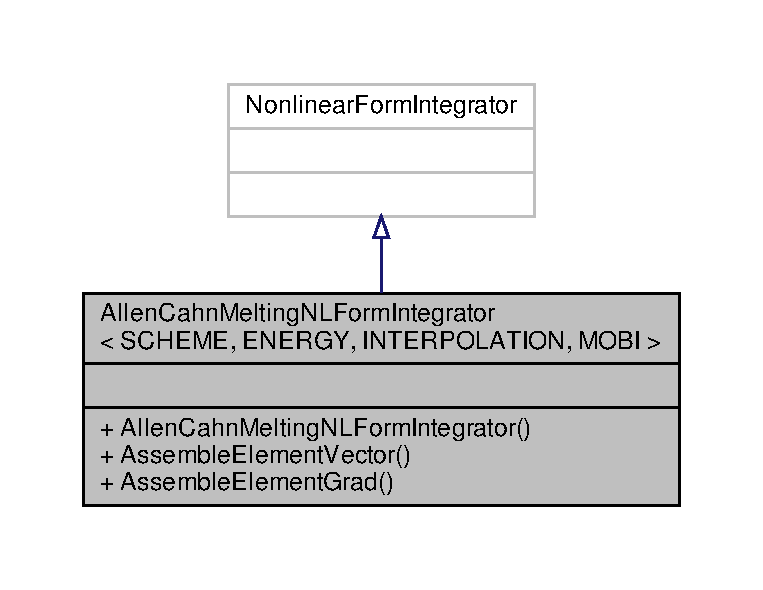
\includegraphics[width=350pt]{classAllenCahnMeltingNLFormIntegrator__inherit__graph}
\end{center}
\end{figure}


Collaboration diagram for Allen\+Cahn\+Melting\+N\+L\+Form\+Integrator$<$ S\+C\+H\+E\+ME, E\+N\+E\+R\+GY, I\+N\+T\+E\+R\+P\+O\+L\+A\+T\+I\+ON, M\+O\+BI $>$\+:\nopagebreak
\begin{figure}[H]
\begin{center}
\leavevmode
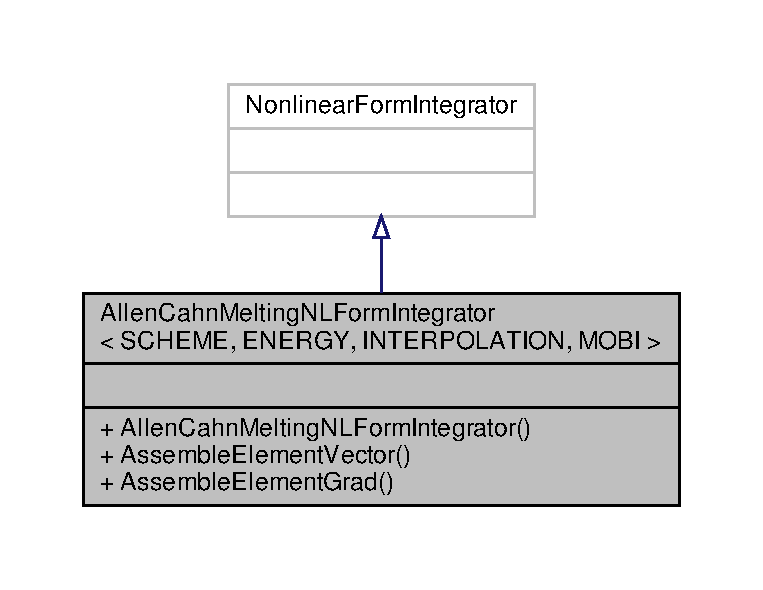
\includegraphics[width=350pt]{classAllenCahnMeltingNLFormIntegrator__coll__graph}
\end{center}
\end{figure}
\subsection*{Public Member Functions}
\begin{DoxyCompactItemize}
\item 
\hyperlink{classAllenCahnMeltingNLFormIntegrator_a56ffb7b7b6963cf1cf8060e82361d861}{Allen\+Cahn\+Melting\+N\+L\+Form\+Integrator} (const mfem\+::\+Grid\+Function \&\+\_\+u\+\_\+old, const double \&\+\_\+omega, const double \&\+\_\+lambda, const double \&\+\_\+mob, \hyperlink{classPhaseChangeCoefficient}{Phase\+Change\+Coefficient} \+\_\+alpha)
\begin{DoxyCompactList}\small\item\em Construct. \end{DoxyCompactList}\item 
virtual void \hyperlink{classAllenCahnMeltingNLFormIntegrator_ab8e7696b5052bda3c43f95f67f0b798f}{Assemble\+Element\+Vector} (const mfem\+::\+Finite\+Element \&el, mfem\+::\+Element\+Transformation \&Tr, const mfem\+::\+Vector \&elfun, mfem\+::\+Vector \&elvect)
\begin{DoxyCompactList}\small\item\em Residual part of the non linear problem. \end{DoxyCompactList}\item 
virtual void \hyperlink{classAllenCahnMeltingNLFormIntegrator_a017da5aa8e63fb3d5c4ec65e721c957e}{Assemble\+Element\+Grad} (const mfem\+::\+Finite\+Element \&el, mfem\+::\+Element\+Transformation \&Tr, const mfem\+::\+Vector \&elfun, mfem\+::\+Dense\+Matrix \&elmat)
\begin{DoxyCompactList}\small\item\em Jacobian part of the non linear problem. \end{DoxyCompactList}\end{DoxyCompactItemize}


\subsection{Detailed Description}
\subsubsection*{template$<$Thermodynamics\+Potential\+Discretization S\+C\+H\+E\+ME, Thermodynamics\+Potentials E\+N\+E\+R\+GY, Thermodynamics\+Potentials I\+N\+T\+E\+R\+P\+O\+L\+A\+T\+I\+ON, Mobility M\+O\+BI$>$\newline
class Allen\+Cahn\+Melting\+N\+L\+Form\+Integrator$<$ S\+C\+H\+E\+M\+E, E\+N\+E\+R\+G\+Y, I\+N\+T\+E\+R\+P\+O\+L\+A\+T\+I\+O\+N, M\+O\+B\+I $>$}



Definition at line 19 of file Allen\+Cahn\+Melting\+N\+L\+Form\+Integrator.\+hpp.



\subsection{Constructor \& Destructor Documentation}
\mbox{\Hypertarget{classAllenCahnMeltingNLFormIntegrator_a56ffb7b7b6963cf1cf8060e82361d861}\label{classAllenCahnMeltingNLFormIntegrator_a56ffb7b7b6963cf1cf8060e82361d861}} 
\index{Allen\+Cahn\+Melting\+N\+L\+Form\+Integrator@{Allen\+Cahn\+Melting\+N\+L\+Form\+Integrator}!Allen\+Cahn\+Melting\+N\+L\+Form\+Integrator@{Allen\+Cahn\+Melting\+N\+L\+Form\+Integrator}}
\index{Allen\+Cahn\+Melting\+N\+L\+Form\+Integrator@{Allen\+Cahn\+Melting\+N\+L\+Form\+Integrator}!Allen\+Cahn\+Melting\+N\+L\+Form\+Integrator@{Allen\+Cahn\+Melting\+N\+L\+Form\+Integrator}}
\subsubsection{\texorpdfstring{Allen\+Cahn\+Melting\+N\+L\+Form\+Integrator()}{AllenCahnMeltingNLFormIntegrator()}}
{\footnotesize\ttfamily template$<$Thermodynamics\+Potential\+Discretization S\+C\+H\+E\+ME, Thermodynamics\+Potentials E\+N\+E\+R\+GY, Thermodynamics\+Potentials I\+N\+T\+E\+R\+P\+O\+L\+A\+T\+I\+ON, Mobility M\+O\+BI$>$ \\
\hyperlink{classAllenCahnMeltingNLFormIntegrator}{Allen\+Cahn\+Melting\+N\+L\+Form\+Integrator}$<$ S\+C\+H\+E\+ME, E\+N\+E\+R\+GY, I\+N\+T\+E\+R\+P\+O\+L\+A\+T\+I\+ON, M\+O\+BI $>$\+::\hyperlink{classAllenCahnMeltingNLFormIntegrator}{Allen\+Cahn\+Melting\+N\+L\+Form\+Integrator} (\begin{DoxyParamCaption}\item[{const mfem\+::\+Grid\+Function \&}]{\+\_\+u\+\_\+old,  }\item[{const double \&}]{\+\_\+omega,  }\item[{const double \&}]{\+\_\+lambda,  }\item[{const double \&}]{\+\_\+mob,  }\item[{\hyperlink{classPhaseChangeCoefficient}{Phase\+Change\+Coefficient}}]{\+\_\+alpha }\end{DoxyParamCaption})}



Construct. 


\begin{DoxyTemplParams}{Template Parameters}
{\em S\+C\+H\+E\+ME} & \\
\hline
{\em E\+N\+E\+R\+GY} & \\
\hline
{\em I\+N\+T\+E\+R\+P\+O\+L\+A\+T\+I\+ON} & \\
\hline
\end{DoxyTemplParams}

\begin{DoxyParams}{Parameters}
{\em \+\_\+u\+\_\+old} & \\
\hline
{\em \+\_\+omega} & \\
\hline
{\em \+\_\+lambda} & \\
\hline
{\em \+\_\+alpha} & \\
\hline
{\em \+\_\+mob} & \\
\hline
\end{DoxyParams}
\begin{DoxyReturn}{Returns}
Allen\+Cahn\+Melting\+N\+L\+Form\+Integrator$<$\+S\+C\+H\+E\+M\+E, E\+N\+E\+R\+G\+Y, I\+N\+T\+E\+R\+P\+O\+L\+A\+T\+I\+O\+N$>$\+:\+: 
\end{DoxyReturn}


Definition at line 71 of file Allen\+Cahn\+Melting\+N\+L\+Form\+Integrator.\+hpp.


\begin{DoxyCode}
74     : u\_old(\_u\_old), omega(\_omega), lambda(\_lambda), mob\_(\_mob), alpha\_(\_alpha) \{\}
\end{DoxyCode}


\subsection{Member Function Documentation}
\mbox{\Hypertarget{classAllenCahnMeltingNLFormIntegrator_a017da5aa8e63fb3d5c4ec65e721c957e}\label{classAllenCahnMeltingNLFormIntegrator_a017da5aa8e63fb3d5c4ec65e721c957e}} 
\index{Allen\+Cahn\+Melting\+N\+L\+Form\+Integrator@{Allen\+Cahn\+Melting\+N\+L\+Form\+Integrator}!Assemble\+Element\+Grad@{Assemble\+Element\+Grad}}
\index{Assemble\+Element\+Grad@{Assemble\+Element\+Grad}!Allen\+Cahn\+Melting\+N\+L\+Form\+Integrator@{Allen\+Cahn\+Melting\+N\+L\+Form\+Integrator}}
\subsubsection{\texorpdfstring{Assemble\+Element\+Grad()}{AssembleElementGrad()}}
{\footnotesize\ttfamily template$<$Thermodynamics\+Potential\+Discretization S\+C\+H\+E\+ME, Thermodynamics\+Potentials E\+N\+E\+R\+GY, Thermodynamics\+Potentials I\+N\+T\+E\+R\+P\+O\+L\+A\+T\+I\+ON, Mobility M\+O\+BI$>$ \\
void \hyperlink{classAllenCahnMeltingNLFormIntegrator}{Allen\+Cahn\+Melting\+N\+L\+Form\+Integrator}$<$ S\+C\+H\+E\+ME, E\+N\+E\+R\+GY, I\+N\+T\+E\+R\+P\+O\+L\+A\+T\+I\+ON, M\+O\+BI $>$\+::Assemble\+Element\+Grad (\begin{DoxyParamCaption}\item[{const mfem\+::\+Finite\+Element \&}]{el,  }\item[{mfem\+::\+Element\+Transformation \&}]{Tr,  }\item[{const mfem\+::\+Vector \&}]{elfun,  }\item[{mfem\+::\+Dense\+Matrix \&}]{elmat }\end{DoxyParamCaption})\hspace{0.3cm}{\ttfamily [virtual]}}



Jacobian part of the non linear problem. 


\begin{DoxyTemplParams}{Template Parameters}
{\em S\+C\+H\+E\+ME} & \\
\hline
{\em E\+N\+E\+R\+GY} & \\
\hline
{\em I\+N\+T\+E\+R\+P\+O\+L\+A\+T\+I\+ON} & \\
\hline
\end{DoxyTemplParams}

\begin{DoxyParams}{Parameters}
{\em el} & \\
\hline
{\em Tr} & \\
\hline
{\em elfun} & \\
\hline
{\em elmat} & \\
\hline
\end{DoxyParams}


Definition at line 161 of file Allen\+Cahn\+Melting\+N\+L\+Form\+Integrator.\+hpp.


\begin{DoxyCode}
163                             \{
164   \textcolor{keywordtype}{int} nd = el.GetDof();
165   \textcolor{keywordtype}{int} dim = el.GetDim();
166   \textcolor{keywordtype}{int} spaceDim = Tr.GetSpaceDim();
167   \textcolor{keywordtype}{bool} square = (dim == spaceDim);
168   \textcolor{keywordtype}{double} w;
169 
170   shape.SetSize(nd);
171   dshape.SetSize(nd, dim);
172   dshapedxt.SetSize(nd, spaceDim);
173   elmat.SetSize(nd);
174 
175   \textcolor{keyword}{const} mfem::IntegrationRule* ir =
176       &mfem::IntRules.Get(el.GetGeomType(), 2 * el.GetOrder() + Tr.OrderW());
177 
178   elmat = 0.0;
179   \textcolor{keywordflow}{for} (\textcolor{keywordtype}{int} i = 0; i < ir->GetNPoints(); i++) \{
180     \textcolor{keyword}{const} mfem::IntegrationPoint& ip = ir->IntPoint(i);
181     el.CalcDShape(ip, dshape);  \textcolor{comment}{// dphi}
182     \textcolor{keyword}{const} \textcolor{keyword}{auto} u = elfun * shape;
183     \textcolor{keyword}{const} \textcolor{keyword}{auto} un = u\_old.GetValue(Tr, ip);
184 
185     \textcolor{keyword}{const} \textcolor{keyword}{auto} W = this->energy\_second\_derivative\_potential\_.
      \hyperlink{classPotentialFunctions_af7b46074a256a70b110ae621d0335874}{getPotentialFunction}(un);
186     \textcolor{keyword}{const} \textcolor{keyword}{auto} H = this->interpolation\_second\_derivative\_potential\_.
      \hyperlink{classPotentialFunctions_af7b46074a256a70b110ae621d0335874}{getPotentialFunction}(un);
187     \textcolor{keyword}{const} \textcolor{keyword}{auto} Wsecond = W(u);
188     \textcolor{keyword}{const} \textcolor{keyword}{auto} Hsecond = H(u);
189     \textcolor{keyword}{const} \textcolor{keyword}{auto} MOB = this->mobility\_function\_.getMobilityFunction(un);
190     \textcolor{keyword}{const} \textcolor{keyword}{auto} Mphi = MOB(this->mob\_);
191     \textcolor{keyword}{const} \textcolor{keyword}{auto} phase\_change = this->alpha\_.Eval(Tr, ip);
192 
193     Tr.SetIntPoint(&ip);
194     w = Tr.Weight();  \textcolor{comment}{// det(J)}
195     \textcolor{comment}{// std::cout << " SQUARE  ? " << square << std::endl;}
196     w = ip.weight / (square ? w : w * w * w);
197     \textcolor{comment}{// AdjugateJacobian = / adj(J),         if J is square}
198     \textcolor{comment}{//                    \(\backslash\) adj(J^t.J).J^t, otherwise}
199 
200     \textcolor{comment}{// Tr.AdjugateJacobian() det(J)J-1}
201 
202     \textcolor{comment}{// w = w* Mphi * lambda}
203     w *= Mphi * this->lambda;
204 
205     \textcolor{comment}{// dshapedxt =  det(J)J-1 dshape}
206     Mult(dshape, Tr.AdjugateJacobian(), dshapedxt);
207     \textcolor{comment}{// elmat += w * dshapedxt * dshapedxt^T}
208     AddMult\_a\_AAt(w, dshapedxt, elmat);
209 
210     \textcolor{comment}{//  (this->omega * secondDerivativedoubleWellPotential(elfun * shape) +}
211     \textcolor{comment}{//   this->alpha * secondDerivativeInterpolationPotential(elfun * shape)) *}
212     \textcolor{comment}{// Compute w'(u)*(du,v), v is shape function}
213     \textcolor{keywordtype}{double} fun\_val =
214         Mphi * (this->omega * Wsecond + phase\_change * Hsecond) * ip.weight * Tr.Weight();  \textcolor{comment}{// w'(u)}
215     \textcolor{comment}{// elmat += fun\_val * shape * shape^T}
216     AddMult\_a\_VVt(fun\_val, shape, elmat);  \textcolor{comment}{// w'(u)*(du, v)}
217   \}
218 \}
\end{DoxyCode}
\mbox{\Hypertarget{classAllenCahnMeltingNLFormIntegrator_ab8e7696b5052bda3c43f95f67f0b798f}\label{classAllenCahnMeltingNLFormIntegrator_ab8e7696b5052bda3c43f95f67f0b798f}} 
\index{Allen\+Cahn\+Melting\+N\+L\+Form\+Integrator@{Allen\+Cahn\+Melting\+N\+L\+Form\+Integrator}!Assemble\+Element\+Vector@{Assemble\+Element\+Vector}}
\index{Assemble\+Element\+Vector@{Assemble\+Element\+Vector}!Allen\+Cahn\+Melting\+N\+L\+Form\+Integrator@{Allen\+Cahn\+Melting\+N\+L\+Form\+Integrator}}
\subsubsection{\texorpdfstring{Assemble\+Element\+Vector()}{AssembleElementVector()}}
{\footnotesize\ttfamily template$<$Thermodynamics\+Potential\+Discretization S\+C\+H\+E\+ME, Thermodynamics\+Potentials E\+N\+E\+R\+GY, Thermodynamics\+Potentials I\+N\+T\+E\+R\+P\+O\+L\+A\+T\+I\+ON, Mobility M\+O\+BI$>$ \\
void \hyperlink{classAllenCahnMeltingNLFormIntegrator}{Allen\+Cahn\+Melting\+N\+L\+Form\+Integrator}$<$ S\+C\+H\+E\+ME, E\+N\+E\+R\+GY, I\+N\+T\+E\+R\+P\+O\+L\+A\+T\+I\+ON, M\+O\+BI $>$\+::Assemble\+Element\+Vector (\begin{DoxyParamCaption}\item[{const mfem\+::\+Finite\+Element \&}]{el,  }\item[{mfem\+::\+Element\+Transformation \&}]{Tr,  }\item[{const mfem\+::\+Vector \&}]{elfun,  }\item[{mfem\+::\+Vector \&}]{elvect }\end{DoxyParamCaption})\hspace{0.3cm}{\ttfamily [virtual]}}



Residual part of the non linear problem. 


\begin{DoxyTemplParams}{Template Parameters}
{\em S\+C\+H\+E\+ME} & \\
\hline
{\em E\+N\+E\+R\+GY} & \\
\hline
{\em I\+N\+T\+E\+R\+P\+O\+L\+A\+T\+I\+ON} & \\
\hline
\end{DoxyTemplParams}

\begin{DoxyParams}{Parameters}
{\em el} & \\
\hline
{\em Tr} & \\
\hline
{\em elfun} & \\
\hline
{\em elvect} & \\
\hline
\end{DoxyParams}


Definition at line 89 of file Allen\+Cahn\+Melting\+N\+L\+Form\+Integrator.\+hpp.


\begin{DoxyCode}
91                         \{
92   \textcolor{keywordtype}{int} nd = el.GetDof();
93   \textcolor{keywordtype}{int} dim = el.GetDim();
94   \textcolor{keywordtype}{int} spaceDim = Tr.GetSpaceDim();
95   dshape.SetSize(nd, dim);
96   shape.SetSize(nd);
97   invdfdx.SetSize(dim, spaceDim);
98   vec.SetSize(dim);
99   pointflux.SetSize(spaceDim);
100 
101   elvect.SetSize(nd);
102   \textcolor{keyword}{const} mfem::IntegrationRule* ir =
103       &mfem::IntRules.Get(el.GetGeomType(), 2 * el.GetOrder() + Tr.OrderW());
104 
105   elvect = 0.0;
106   \textcolor{keywordflow}{for} (\textcolor{keywordtype}{int} i = 0; i < ir->GetNPoints(); i++) \{
107     \textcolor{keyword}{const} mfem::IntegrationPoint& ip = ir->IntPoint(i);
108     el.CalcDShape(ip, dshape);  \textcolor{comment}{// dphi}
109     el.CalcShape(ip, shape);    \textcolor{comment}{// phi}
110     Tr.SetIntPoint(&ip);
111 
112     \textcolor{keyword}{const} \textcolor{keyword}{auto} u = elfun * shape;
113     \textcolor{keyword}{const} \textcolor{keyword}{auto} un = u\_old.GetValue(Tr, ip);
114 
115     \textcolor{keyword}{const} \textcolor{keyword}{auto} W = this->energy\_first\_derivative\_potential\_.\hyperlink{classPotentialFunctions_af7b46074a256a70b110ae621d0335874}{getPotentialFunction}(un);
116     \textcolor{keyword}{const} \textcolor{keyword}{auto} H = this->interpolation\_first\_derivative\_potential\_.
      \hyperlink{classPotentialFunctions_af7b46074a256a70b110ae621d0335874}{getPotentialFunction}(un);
117     \textcolor{keyword}{const} \textcolor{keyword}{auto} Wprime = W(u);
118     \textcolor{keyword}{const} \textcolor{keyword}{auto} Hprime = H(u);
119     \textcolor{keyword}{const} \textcolor{keyword}{auto} MOB = this->mobility\_function\_.getMobilityFunction(un);
120     \textcolor{keyword}{const} \textcolor{keyword}{auto} Mphi = MOB(this->mob\_);
121     \textcolor{keyword}{const} \textcolor{keyword}{auto} phase\_change = this->alpha\_.Eval(Tr, ip);
122 
123     CalcAdjugate(Tr.Jacobian(), invdfdx);  \textcolor{comment}{// invdfdx = adj(J)}
124 
125     dshape.MultTranspose(elfun, vec);
126     invdfdx.MultTranspose(vec, pointflux);
127 
128     \textcolor{comment}{// Energy contribution}
129     \textcolor{keyword}{const} \textcolor{keyword}{auto} energy = this->omega * Wprime;
130     \textcolor{comment}{// Enthalpy of melting contribution}
131     \textcolor{keyword}{const} \textcolor{keyword}{auto} enthalpy = phase\_change * Hprime;
132     \textcolor{comment}{// flow of phase change + source term}
133     \textcolor{keyword}{const} \textcolor{keyword}{auto} fun\_val = Mphi * (energy + enthalpy);
134 
135     \textcolor{comment}{// Given phi, compute (w'(phi)-f, v), v is shape function}
136     \textcolor{keyword}{const} \textcolor{keywordtype}{double} ww = ip.weight * Tr.Weight() * fun\_val;
137     add(elvect, ww, shape, elvect);
138 
139     \textcolor{comment}{// Laplacian : given u, compute (grad(u), grad(v)), v is shape function.}
140     \textcolor{keywordtype}{double} w;
141     w = Mphi * ip.weight * this->lambda / Tr.Weight();
142     pointflux *= w;
143     invdfdx.Mult(pointflux, vec);
144     dshape.AddMult(vec, elvect);
145   \}
146 \}
\end{DoxyCode}


The documentation for this class was generated from the following file\+:\begin{DoxyCompactItemize}
\item 
Allen\+Cahn\+Melting\+N\+L\+Form\+Integrator.\+hpp\end{DoxyCompactItemize}

\hypertarget{classAllenCahnNLFormIntegrator}{}\section{Allen\+Cahn\+N\+L\+Form\+Integrator$<$ S\+C\+H\+E\+ME, E\+N\+E\+R\+GY, M\+O\+BI $>$ Class Template Reference}
\label{classAllenCahnNLFormIntegrator}\index{Allen\+Cahn\+N\+L\+Form\+Integrator$<$ S\+C\+H\+E\+M\+E, E\+N\+E\+R\+G\+Y, M\+O\+B\+I $>$@{Allen\+Cahn\+N\+L\+Form\+Integrator$<$ S\+C\+H\+E\+M\+E, E\+N\+E\+R\+G\+Y, M\+O\+B\+I $>$}}


Inheritance diagram for Allen\+Cahn\+N\+L\+Form\+Integrator$<$ S\+C\+H\+E\+ME, E\+N\+E\+R\+GY, M\+O\+BI $>$\+:\nopagebreak
\begin{figure}[H]
\begin{center}
\leavevmode
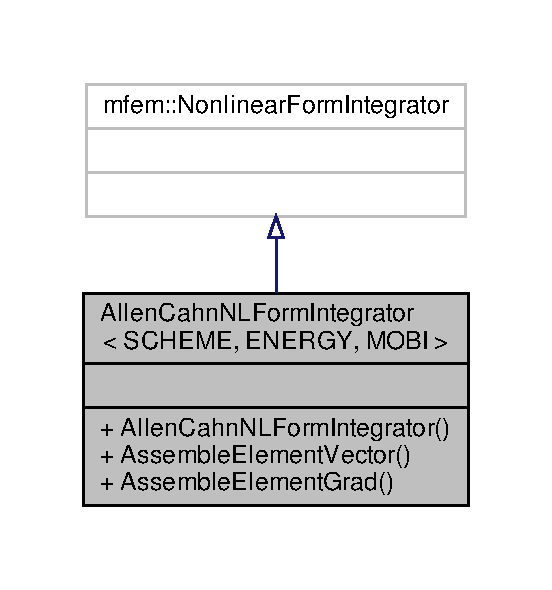
\includegraphics[width=265pt]{classAllenCahnNLFormIntegrator__inherit__graph}
\end{center}
\end{figure}


Collaboration diagram for Allen\+Cahn\+N\+L\+Form\+Integrator$<$ S\+C\+H\+E\+ME, E\+N\+E\+R\+GY, M\+O\+BI $>$\+:\nopagebreak
\begin{figure}[H]
\begin{center}
\leavevmode
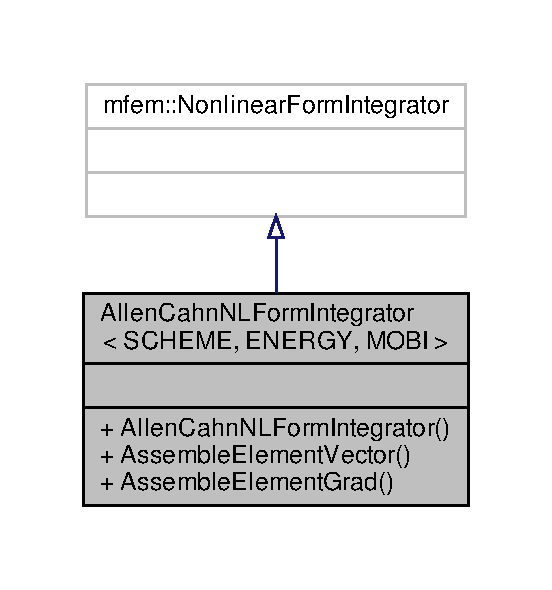
\includegraphics[width=265pt]{classAllenCahnNLFormIntegrator__coll__graph}
\end{center}
\end{figure}
\subsection*{Public Member Functions}
\begin{DoxyCompactItemize}
\item 
\hyperlink{classAllenCahnNLFormIntegrator_aa683f1361b0fb5c0c29848bf020eebd3}{Allen\+Cahn\+N\+L\+Form\+Integrator} (const mfem\+::\+Grid\+Function \&\+\_\+u\+\_\+old, const double \&\+\_\+omega, const double \&\+\_\+lambda, const double \&\+\_\+mob)
\begin{DoxyCompactList}\small\item\em Construct. \end{DoxyCompactList}\item 
virtual void \hyperlink{classAllenCahnNLFormIntegrator_a4cb7cff96ecd5b236ba1573b4fdc816c}{Assemble\+Element\+Vector} (const mfem\+::\+Finite\+Element \&el, mfem\+::\+Element\+Transformation \&Tr, const mfem\+::\+Vector \&elfun, mfem\+::\+Vector \&elvect)
\begin{DoxyCompactList}\small\item\em Residual part of the non linear problem. \end{DoxyCompactList}\item 
virtual void \hyperlink{classAllenCahnNLFormIntegrator_a0370504d306247b934fee91ed117104a}{Assemble\+Element\+Grad} (const mfem\+::\+Finite\+Element \&el, mfem\+::\+Element\+Transformation \&Tr, const mfem\+::\+Vector \&elfun, mfem\+::\+Dense\+Matrix \&elmat)
\begin{DoxyCompactList}\small\item\em Jacobian part of the non linear problem. \end{DoxyCompactList}\end{DoxyCompactItemize}


\subsection{Detailed Description}
\subsubsection*{template$<$Thermodynamics\+Potential\+Discretization S\+C\+H\+E\+ME, Thermodynamics\+Potentials E\+N\+E\+R\+GY, Mobility M\+O\+BI$>$\newline
class Allen\+Cahn\+N\+L\+Form\+Integrator$<$ S\+C\+H\+E\+M\+E, E\+N\+E\+R\+G\+Y, M\+O\+B\+I $>$}



Definition at line 18 of file Allen\+Cahn\+N\+L\+Form\+Integrator.\+hpp.



\subsection{Constructor \& Destructor Documentation}
\mbox{\Hypertarget{classAllenCahnNLFormIntegrator_aa683f1361b0fb5c0c29848bf020eebd3}\label{classAllenCahnNLFormIntegrator_aa683f1361b0fb5c0c29848bf020eebd3}} 
\index{Allen\+Cahn\+N\+L\+Form\+Integrator@{Allen\+Cahn\+N\+L\+Form\+Integrator}!Allen\+Cahn\+N\+L\+Form\+Integrator@{Allen\+Cahn\+N\+L\+Form\+Integrator}}
\index{Allen\+Cahn\+N\+L\+Form\+Integrator@{Allen\+Cahn\+N\+L\+Form\+Integrator}!Allen\+Cahn\+N\+L\+Form\+Integrator@{Allen\+Cahn\+N\+L\+Form\+Integrator}}
\subsubsection{\texorpdfstring{Allen\+Cahn\+N\+L\+Form\+Integrator()}{AllenCahnNLFormIntegrator()}}
{\footnotesize\ttfamily template$<$Thermodynamics\+Potential\+Discretization S\+C\+H\+E\+ME, Thermodynamics\+Potentials E\+N\+E\+R\+GY, Mobility M\+O\+BI$>$ \\
\hyperlink{classAllenCahnNLFormIntegrator}{Allen\+Cahn\+N\+L\+Form\+Integrator}$<$ S\+C\+H\+E\+ME, E\+N\+E\+R\+GY, M\+O\+BI $>$\+::\hyperlink{classAllenCahnNLFormIntegrator}{Allen\+Cahn\+N\+L\+Form\+Integrator} (\begin{DoxyParamCaption}\item[{const mfem\+::\+Grid\+Function \&}]{\+\_\+u\+\_\+old,  }\item[{const double \&}]{\+\_\+omega,  }\item[{const double \&}]{\+\_\+lambda,  }\item[{const double \&}]{\+\_\+mob }\end{DoxyParamCaption})}



Construct. 


\begin{DoxyTemplParams}{Template Parameters}
{\em S\+C\+H\+E\+ME} & \\
\hline
{\em E\+N\+E\+R\+GY} & \\
\hline
\end{DoxyTemplParams}

\begin{DoxyParams}{Parameters}
{\em \+\_\+u\+\_\+old} & \\
\hline
{\em \+\_\+omega} & \\
\hline
{\em \+\_\+lambda} & \\
\hline
{\em \+\_\+alpha} & \\
\hline
{\em \+\_\+mob} & \\
\hline
\end{DoxyParams}
\begin{DoxyReturn}{Returns}
Allen\+Cahn\+N\+L\+Form\+Integrator$<$\+S\+C\+H\+E\+M\+E, E\+N\+E\+R\+G\+Y$>$\+:\+: 
\end{DoxyReturn}


Definition at line 62 of file Allen\+Cahn\+N\+L\+Form\+Integrator.\+hpp.


\begin{DoxyCode}
65     : u\_old(\_u\_old), omega(\_omega), lambda(\_lambda), mob\_(\_mob) \{\}
\end{DoxyCode}


\subsection{Member Function Documentation}
\mbox{\Hypertarget{classAllenCahnNLFormIntegrator_a0370504d306247b934fee91ed117104a}\label{classAllenCahnNLFormIntegrator_a0370504d306247b934fee91ed117104a}} 
\index{Allen\+Cahn\+N\+L\+Form\+Integrator@{Allen\+Cahn\+N\+L\+Form\+Integrator}!Assemble\+Element\+Grad@{Assemble\+Element\+Grad}}
\index{Assemble\+Element\+Grad@{Assemble\+Element\+Grad}!Allen\+Cahn\+N\+L\+Form\+Integrator@{Allen\+Cahn\+N\+L\+Form\+Integrator}}
\subsubsection{\texorpdfstring{Assemble\+Element\+Grad()}{AssembleElementGrad()}}
{\footnotesize\ttfamily template$<$Thermodynamics\+Potential\+Discretization S\+C\+H\+E\+ME, Thermodynamics\+Potentials E\+N\+E\+R\+GY, Mobility M\+O\+BI$>$ \\
void \hyperlink{classAllenCahnNLFormIntegrator}{Allen\+Cahn\+N\+L\+Form\+Integrator}$<$ S\+C\+H\+E\+ME, E\+N\+E\+R\+GY, M\+O\+BI $>$\+::Assemble\+Element\+Grad (\begin{DoxyParamCaption}\item[{const mfem\+::\+Finite\+Element \&}]{el,  }\item[{mfem\+::\+Element\+Transformation \&}]{Tr,  }\item[{const mfem\+::\+Vector \&}]{elfun,  }\item[{mfem\+::\+Dense\+Matrix \&}]{elmat }\end{DoxyParamCaption})\hspace{0.3cm}{\ttfamily [virtual]}}



Jacobian part of the non linear problem. 


\begin{DoxyTemplParams}{Template Parameters}
{\em S\+C\+H\+E\+ME} & \\
\hline
{\em E\+N\+E\+R\+GY} & \\
\hline
\end{DoxyTemplParams}

\begin{DoxyParams}{Parameters}
{\em el} & \\
\hline
{\em Tr} & \\
\hline
{\em elfun} & \\
\hline
{\em elmat} & \\
\hline
\end{DoxyParams}


Definition at line 143 of file Allen\+Cahn\+N\+L\+Form\+Integrator.\+hpp.


\begin{DoxyCode}
145                             \{
146   \textcolor{keywordtype}{int} nd = el.GetDof();
147   \textcolor{keywordtype}{int} dim = el.GetDim();
148   \textcolor{keywordtype}{int} spaceDim = Tr.GetSpaceDim();
149   \textcolor{keywordtype}{bool} square = (dim == spaceDim);
150   \textcolor{keywordtype}{double} w;
151 
152   shape.SetSize(nd);
153   dshape.SetSize(nd, dim);
154   dshapedxt.SetSize(nd, spaceDim);
155   elmat.SetSize(nd);
156 
157   \textcolor{keyword}{const} mfem::IntegrationRule* ir =
158       &mfem::IntRules.Get(el.GetGeomType(), 2 * el.GetOrder() + Tr.OrderW());
159 
160   elmat = 0.0;
161   \textcolor{keywordflow}{for} (\textcolor{keywordtype}{int} i = 0; i < ir->GetNPoints(); i++) \{
162     \textcolor{keyword}{const} mfem::IntegrationPoint& ip = ir->IntPoint(i);
163     el.CalcDShape(ip, dshape);  \textcolor{comment}{// dphi}
164     \textcolor{keyword}{const} \textcolor{keyword}{auto} u = elfun * shape;
165     \textcolor{keyword}{const} \textcolor{keyword}{auto} un = u\_old.GetValue(Tr, ip);
166 
167     \textcolor{keyword}{const} \textcolor{keyword}{auto} W = this->energy\_second\_derivative\_potential\_.
      \hyperlink{classPotentialFunctions_af7b46074a256a70b110ae621d0335874}{getPotentialFunction}(un);
168     \textcolor{keyword}{const} \textcolor{keyword}{auto} Wsecond = W(u);
169     \textcolor{keyword}{const} \textcolor{keyword}{auto} MOB = this->mobility\_function\_.getMobilityFunction(un);
170     \textcolor{keyword}{const} \textcolor{keyword}{auto} Mphi = MOB(this->mob\_);
171 
172     Tr.SetIntPoint(&ip);
173     w = Tr.Weight();  \textcolor{comment}{// det(J)}
174     \textcolor{comment}{// std::cout << " SQUARE  ? " << square << std::endl;}
175     w = ip.weight / (square ? w : w * w * w);
176     \textcolor{comment}{// AdjugateJacobian = / adj(J),         if J is square}
177     \textcolor{comment}{//                    \(\backslash\) adj(J^t.J).J^t, otherwise}
178 
179     \textcolor{comment}{// Tr.AdjugateJacobian() det(J)J-1}
180 
181     w *= Mphi * this->lambda;
182 
183     \textcolor{comment}{// dshapedxt =  det(J)J-1 dshape}
184     Mult(dshape, Tr.AdjugateJacobian(), dshapedxt);
185     \textcolor{comment}{// elmat += w * dshapedxt * dshapedxt^T}
186     AddMult\_a\_AAt(w, dshapedxt, elmat);
187 
188     \textcolor{comment}{//  (this->omega * secondDerivativedoubleWellPotential(elfun * shape) +}
189     \textcolor{comment}{//   this->alpha * secondDerivativeInterpolationPotential(elfun * shape)) *}
190     \textcolor{comment}{// Compute w'(u)*(du,v), v is shape function}
191     \textcolor{keywordtype}{double} fun\_val = (Mphi * this->omega * Wsecond) * ip.weight * Tr.Weight();  \textcolor{comment}{// w'(u)}
192     \textcolor{comment}{// elmat += fun\_val * shape * shape^T}
193     AddMult\_a\_VVt(fun\_val, shape, elmat);  \textcolor{comment}{// w'(u)*(du, v)}
194   \}
195 \}
\end{DoxyCode}
\mbox{\Hypertarget{classAllenCahnNLFormIntegrator_a4cb7cff96ecd5b236ba1573b4fdc816c}\label{classAllenCahnNLFormIntegrator_a4cb7cff96ecd5b236ba1573b4fdc816c}} 
\index{Allen\+Cahn\+N\+L\+Form\+Integrator@{Allen\+Cahn\+N\+L\+Form\+Integrator}!Assemble\+Element\+Vector@{Assemble\+Element\+Vector}}
\index{Assemble\+Element\+Vector@{Assemble\+Element\+Vector}!Allen\+Cahn\+N\+L\+Form\+Integrator@{Allen\+Cahn\+N\+L\+Form\+Integrator}}
\subsubsection{\texorpdfstring{Assemble\+Element\+Vector()}{AssembleElementVector()}}
{\footnotesize\ttfamily template$<$Thermodynamics\+Potential\+Discretization S\+C\+H\+E\+ME, Thermodynamics\+Potentials E\+N\+E\+R\+GY, Mobility M\+O\+BI$>$ \\
void \hyperlink{classAllenCahnNLFormIntegrator}{Allen\+Cahn\+N\+L\+Form\+Integrator}$<$ S\+C\+H\+E\+ME, E\+N\+E\+R\+GY, M\+O\+BI $>$\+::Assemble\+Element\+Vector (\begin{DoxyParamCaption}\item[{const mfem\+::\+Finite\+Element \&}]{el,  }\item[{mfem\+::\+Element\+Transformation \&}]{Tr,  }\item[{const mfem\+::\+Vector \&}]{elfun,  }\item[{mfem\+::\+Vector \&}]{elvect }\end{DoxyParamCaption})\hspace{0.3cm}{\ttfamily [virtual]}}



Residual part of the non linear problem. 


\begin{DoxyTemplParams}{Template Parameters}
{\em S\+C\+H\+E\+ME} & \\
\hline
{\em E\+N\+E\+R\+GY} & \\
\hline
\end{DoxyTemplParams}

\begin{DoxyParams}{Parameters}
{\em el} & \\
\hline
{\em Tr} & \\
\hline
{\em elfun} & \\
\hline
{\em elvect} & \\
\hline
\end{DoxyParams}


Definition at line 79 of file Allen\+Cahn\+N\+L\+Form\+Integrator.\+hpp.


\begin{DoxyCode}
81                         \{
82   \textcolor{keywordtype}{int} nd = el.GetDof();
83   \textcolor{keywordtype}{int} dim = el.GetDim();
84   \textcolor{keywordtype}{int} spaceDim = Tr.GetSpaceDim();
85   dshape.SetSize(nd, dim);
86   shape.SetSize(nd);
87   invdfdx.SetSize(dim, spaceDim);
88   vec.SetSize(dim);
89   pointflux.SetSize(spaceDim);
90 
91   elvect.SetSize(nd);
92   \textcolor{keyword}{const} mfem::IntegrationRule* ir =
93       &mfem::IntRules.Get(el.GetGeomType(), 2 * el.GetOrder() + Tr.OrderW());
94   elvect = 0.0;
95   \textcolor{keywordflow}{for} (\textcolor{keywordtype}{int} i = 0; i < ir->GetNPoints(); i++) \{
96     \textcolor{keyword}{const} mfem::IntegrationPoint& ip = ir->IntPoint(i);
97     el.CalcDShape(ip, dshape);  \textcolor{comment}{// dphi}
98     el.CalcShape(ip, shape);    \textcolor{comment}{// phi}
99     Tr.SetIntPoint(&ip);
100 
101     \textcolor{keyword}{const} \textcolor{keyword}{auto} u = elfun * shape;
102     \textcolor{keyword}{const} \textcolor{keyword}{auto} un = u\_old.GetValue(Tr, ip);
103 
104     \textcolor{keyword}{const} \textcolor{keyword}{auto} W = this->energy\_first\_derivative\_potential\_.\hyperlink{classPotentialFunctions_af7b46074a256a70b110ae621d0335874}{getPotentialFunction}(un);
105     \textcolor{keyword}{const} \textcolor{keyword}{auto} Wprime = W(u);
106     \textcolor{keyword}{const} \textcolor{keyword}{auto} MOB = this->mobility\_function\_.getMobilityFunction(un);
107     \textcolor{keyword}{const} \textcolor{keyword}{auto} Mphi = MOB(this->mob\_);
108 
109     CalcAdjugate(Tr.Jacobian(), invdfdx);  \textcolor{comment}{// invdfdx = adj(J)}
110 
111     dshape.MultTranspose(elfun, vec);
112     invdfdx.MultTranspose(vec, pointflux);
113 
114     \textcolor{comment}{// Energy contribution + source}
115     \textcolor{keyword}{const} \textcolor{keyword}{auto} energy = this->omega * Wprime;
116     \textcolor{keyword}{const} \textcolor{keyword}{auto} fun\_val = Mphi * energy;
117 
118     \textcolor{comment}{// Given phi, compute (w'(phi)-f, v), v is shape function}
119     \textcolor{keyword}{const} \textcolor{keywordtype}{double} ww = ip.weight * Tr.Weight() * fun\_val;
120     add(elvect, ww, shape, elvect);
121 
122     \textcolor{comment}{// Laplacian : given u, compute (grad(u), grad(v)), v is shape function.}
123     \textcolor{keywordtype}{double} w;
124     w = Mphi * ip.weight * this->lambda / Tr.Weight();
125     pointflux *= w;
126     invdfdx.Mult(pointflux, vec);
127     dshape.AddMult(vec, elvect);
128   \}
129 \}
\end{DoxyCode}


The documentation for this class was generated from the following file\+:\begin{DoxyCompactItemize}
\item 
Allen\+Cahn\+N\+L\+Form\+Integrator.\+hpp\end{DoxyCompactItemize}

\hypertarget{classAnalyticalFunctions}{}\section{Analytical\+Functions$<$ D\+IM $>$ Class Template Reference}
\label{classAnalyticalFunctions}\index{Analytical\+Functions$<$ D\+I\+M $>$@{Analytical\+Functions$<$ D\+I\+M $>$}}


Collaboration diagram for Analytical\+Functions$<$ D\+IM $>$\+:\nopagebreak
\begin{figure}[H]
\begin{center}
\leavevmode
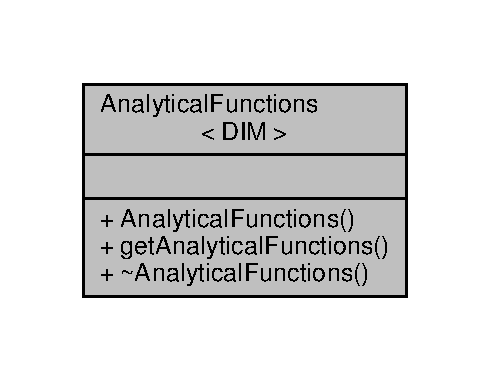
\includegraphics[width=235pt]{classAnalyticalFunctions__coll__graph}
\end{center}
\end{figure}
\subsection*{Public Member Functions}
\begin{DoxyCompactItemize}
\item 
\mbox{\Hypertarget{classAnalyticalFunctions_a6474690b4e60e8d3e55fc12d46752144}\label{classAnalyticalFunctions_a6474690b4e60e8d3e55fc12d46752144}} 
\hyperlink{classAnalyticalFunctions_a6474690b4e60e8d3e55fc12d46752144}{Analytical\+Functions} ()
\begin{DoxyCompactList}\small\item\em Construct a new analytical function\+:\+: analytical function object. \end{DoxyCompactList}\item 
{\footnotesize template$<$typename... Args$>$ }\\std\+::function$<$ double(const mfem\+::\+Vector \&, double)$>$ \hyperlink{classAnalyticalFunctions_a88a27c868b872e12d16f1097779fd3f8}{get\+Analytical\+Functions} (const std\+::string \&analytical\+\_\+function\+\_\+name, Args... args)
\begin{DoxyCompactList}\small\item\em return the function associated with the analytical\+\_\+function\+\_\+name \end{DoxyCompactList}\item 
\mbox{\Hypertarget{classAnalyticalFunctions_a937c9536543c324e57dfab404846d55b}\label{classAnalyticalFunctions_a937c9536543c324e57dfab404846d55b}} 
\hyperlink{classAnalyticalFunctions_a937c9536543c324e57dfab404846d55b}{$\sim$\+Analytical\+Functions} ()
\begin{DoxyCompactList}\small\item\em Destroy the analytical function \+:\+: analytical function object. \end{DoxyCompactList}\end{DoxyCompactItemize}


\subsection{Detailed Description}
\subsubsection*{template$<$int D\+IM$>$\newline
class Analytical\+Functions$<$ D\+I\+M $>$}



Definition at line 24 of file Utils/\+Analytical\+Functions.\+hpp.



\subsection{Member Function Documentation}
\mbox{\Hypertarget{classAnalyticalFunctions_a88a27c868b872e12d16f1097779fd3f8}\label{classAnalyticalFunctions_a88a27c868b872e12d16f1097779fd3f8}} 
\index{Analytical\+Functions@{Analytical\+Functions}!get\+Analytical\+Functions@{get\+Analytical\+Functions}}
\index{get\+Analytical\+Functions@{get\+Analytical\+Functions}!Analytical\+Functions@{Analytical\+Functions}}
\subsubsection{\texorpdfstring{get\+Analytical\+Functions()}{getAnalyticalFunctions()}}
{\footnotesize\ttfamily template$<$int D\+IM$>$ \\
template$<$class... Args$>$ \\
std\+::function$<$ double(const mfem\+::\+Vector \&, double)$>$ \hyperlink{classAnalyticalFunctions}{Analytical\+Functions}$<$ D\+IM $>$\+::get\+Analytical\+Functions (\begin{DoxyParamCaption}\item[{const std\+::string \&}]{analytical\+\_\+function\+\_\+name,  }\item[{Args...}]{args }\end{DoxyParamCaption})}



return the function associated with the analytical\+\_\+function\+\_\+name 


\begin{DoxyParams}{Parameters}
{\em analytical\+\_\+function\+\_\+name} & \\
\hline
\end{DoxyParams}
\begin{DoxyReturn}{Returns}
const double 
\end{DoxyReturn}


Definition at line 307 of file Utils/\+Analytical\+Functions.\+hpp.



Referenced by Phase\+Field\+Operator\+Base$<$ T, D\+I\+M, N\+L\+F\+I $>$\+::\+Phase\+Field\+Operator\+Base().


\begin{DoxyCode}
308                                                                \{
309   \textcolor{keywordflow}{switch} (AnalyticalFunctionsType::from(analytical\_function\_name)) \{
310     \textcolor{keywordflow}{case} AnalyticalFunctionsType::Heaviside:
311       \textcolor{keywordflow}{return} this->getHeaviside(args...);
312     \textcolor{keywordflow}{case} AnalyticalFunctionsType::Sinusoide:
313       \textcolor{keywordflow}{return} this->getSinusoide(args...);
314     \textcolor{keywordflow}{case} AnalyticalFunctionsType::Sinusoide2:
315       \textcolor{keywordflow}{return} this->getSinusoide2(args...);
316     \textcolor{keywordflow}{case} AnalyticalFunctionsType::HyperbolicTangent:
317       \textcolor{keywordflow}{return} this->getHyperbolicTangent(args...);
318     \textcolor{keywordflow}{case} AnalyticalFunctionsType::Uniform:
319       \textcolor{keywordflow}{return} this->getUniform(args...);
320     \textcolor{keywordflow}{default}:
321       \textcolor{keywordflow}{throw} std::runtime\_error(
322           \textcolor{stringliteral}{"AnalyticalFunctions::getAnalyticalFunctions: Heaviside, Sinusoide, HyperbolicTangent "}
323           \textcolor{stringliteral}{"and Uniform "}
324           \textcolor{stringliteral}{"analytical function  are available"});
325       \textcolor{keywordflow}{break};
326   \}
327 \}
\end{DoxyCode}


The documentation for this class was generated from the following file\+:\begin{DoxyCompactItemize}
\item 
Utils/\+Analytical\+Functions.\+hpp\end{DoxyCompactItemize}

\hypertarget{structAnalyticalFunctionsType}{}\section{Analytical\+Functions\+Type Struct Reference}
\label{structAnalyticalFunctionsType}\index{Analytical\+Functions\+Type@{Analytical\+Functions\+Type}}


Collaboration diagram for Analytical\+Functions\+Type\+:\nopagebreak
\begin{figure}[H]
\begin{center}
\leavevmode
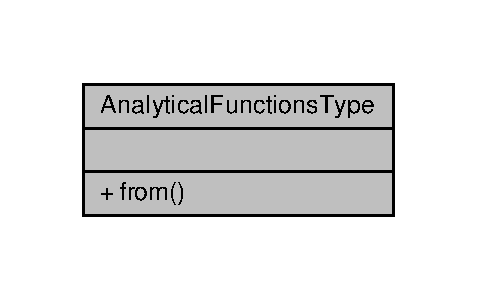
\includegraphics[width=229pt]{structAnalyticalFunctionsType__coll__graph}
\end{center}
\end{figure}
\subsection*{Public Types}
\begin{DoxyCompactItemize}
\item 
\mbox{\Hypertarget{structAnalyticalFunctionsType_a9679669709a07a7255b7f2522af78f2c}\label{structAnalyticalFunctionsType_a9679669709a07a7255b7f2522af78f2c}} 
enum {\bfseries value} \{ \newline
{\bfseries Heaviside}, 
{\bfseries Sinusoide}, 
{\bfseries Sinusoide2}, 
{\bfseries Hyperbolic\+Tangent}, 
\newline
{\bfseries Uniform}
 \}
\end{DoxyCompactItemize}
\subsection*{Static Public Member Functions}
\begin{DoxyCompactItemize}
\item 
\mbox{\Hypertarget{structAnalyticalFunctionsType_a2446df6460acecf21abad99e6b79c3db}\label{structAnalyticalFunctionsType_a2446df6460acecf21abad99e6b79c3db}} 
static value {\bfseries from} (const std\+::string \&)
\end{DoxyCompactItemize}


\subsection{Detailed Description}


Definition at line 75 of file Utils/\+Phase\+Field\+Options.\+hpp.



The documentation for this struct was generated from the following file\+:\begin{DoxyCompactItemize}
\item 
Utils/\+Phase\+Field\+Options.\+hpp\end{DoxyCompactItemize}

\hypertarget{classBoundary}{}\section{Boundary Class Reference}
\label{classBoundary}\index{Boundary@{Boundary}}


Class for defining a boundary with a name, an index, a type and, if needed, a value.  




{\ttfamily \#include $<$/home/ci230846/home-\/local/\+My\+Git\+Projects/\+C\+O\+M\+P\+O\+N\+E\+N\+T/\+P\+F-\/\+M\+F\+E\+M/\+B\+Cs/\+Boundary.\+hpp$>$}



Collaboration diagram for Boundary\+:\nopagebreak
\begin{figure}[H]
\begin{center}
\leavevmode
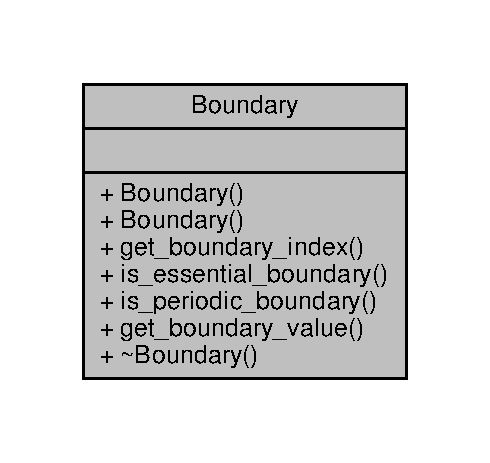
\includegraphics[width=235pt]{classBoundary__coll__graph}
\end{center}
\end{figure}
\subsection*{Public Member Functions}
\begin{DoxyCompactItemize}
\item 
\hyperlink{classBoundary_a145bbf70e6907e3d5ae3a5ac33b4bb2b}{Boundary} (const std\+::string \&boundary\+\_\+name, const int \&boundary\+\_\+index, const std\+::string \&boundary\+\_\+type)
\begin{DoxyCompactList}\small\item\em Construct a new \hyperlink{classBoundary}{Boundary}\+:\+: \hyperlink{classBoundary}{Boundary} object (null value prescribed by default) \end{DoxyCompactList}\item 
\hyperlink{classBoundary_a60ec4ca219af885067b7583a92d2a2d1}{Boundary} (const std\+::string \&boundary\+\_\+name, const int \&boundary\+\_\+index, const std\+::string \&boundary\+\_\+type, const double \&boundary\+\_\+value)
\begin{DoxyCompactList}\small\item\em Construct a new \hyperlink{classBoundary}{Boundary}\+:\+: \hyperlink{classBoundary}{Boundary} object. \end{DoxyCompactList}\item 
int \hyperlink{classBoundary_a8a73f9a2cb9f798a3adc4d9dab58610b}{get\+\_\+boundary\+\_\+index} () const
\begin{DoxyCompactList}\small\item\em return the index associated to the boundary \end{DoxyCompactList}\item 
bool \hyperlink{classBoundary_ab367015ba9c9fc55528032cb5b9eca95}{is\+\_\+essential\+\_\+boundary} () const
\begin{DoxyCompactList}\small\item\em flag to identify essential boundary \end{DoxyCompactList}\item 
bool \hyperlink{classBoundary_a3050c65c13641207ee776309baec08ff}{is\+\_\+periodic\+\_\+boundary} () const
\begin{DoxyCompactList}\small\item\em flag to identify periodic boundary \end{DoxyCompactList}\item 
double \hyperlink{classBoundary_afbd4effd911d4a699bb33d48b5f9396b}{get\+\_\+boundary\+\_\+value} () const
\begin{DoxyCompactList}\small\item\em return the double value prescribed on boundary \end{DoxyCompactList}\item 
\mbox{\Hypertarget{classBoundary_a86eab4f2362618c5b1e3d0df3a5f7f42}\label{classBoundary_a86eab4f2362618c5b1e3d0df3a5f7f42}} 
\hyperlink{classBoundary_a86eab4f2362618c5b1e3d0df3a5f7f42}{$\sim$\+Boundary} ()
\begin{DoxyCompactList}\small\item\em Destroy the \hyperlink{classBoundary}{Boundary}\+:\+: \hyperlink{classBoundary}{Boundary} object. \end{DoxyCompactList}\end{DoxyCompactItemize}


\subsection{Detailed Description}
Class for defining a boundary with a name, an index, a type and, if needed, a value. 

Definition at line 24 of file Boundary.\+hpp.



\subsection{Constructor \& Destructor Documentation}
\mbox{\Hypertarget{classBoundary_a145bbf70e6907e3d5ae3a5ac33b4bb2b}\label{classBoundary_a145bbf70e6907e3d5ae3a5ac33b4bb2b}} 
\index{Boundary@{Boundary}!Boundary@{Boundary}}
\index{Boundary@{Boundary}!Boundary@{Boundary}}
\subsubsection{\texorpdfstring{Boundary()}{Boundary()}\hspace{0.1cm}{\footnotesize\ttfamily [1/2]}}
{\footnotesize\ttfamily Boundary\+::\+Boundary (\begin{DoxyParamCaption}\item[{const std\+::string \&}]{boundary\+\_\+name,  }\item[{const int \&}]{boundary\+\_\+index,  }\item[{const std\+::string \&}]{boundary\+\_\+type }\end{DoxyParamCaption})}



Construct a new \hyperlink{classBoundary}{Boundary}\+:\+: \hyperlink{classBoundary}{Boundary} object (null value prescribed by default) 


\begin{DoxyParams}{Parameters}
{\em boundary\+\_\+name} & \\
\hline
{\em boundary\+\_\+index} & \\
\hline
{\em boundary\+\_\+type} & \\
\hline
\end{DoxyParams}


Definition at line 53 of file Boundary.\+hpp.


\begin{DoxyCode}
55     : boundary\_name\_(boundary\_name), boundary\_index\_(boundary\_index) \{
56   \textcolor{keywordflow}{switch} (BoundaryConditionType::from(boundary\_type)) \{
57     \textcolor{keywordflow}{case} BoundaryConditionType::Dirichlet:
58       this->is\_essential\_boundary\_ = \textcolor{keyword}{true};
59       this->is\_periodic\_boundary\_ = \textcolor{keyword}{false};
60       \textcolor{keywordflow}{break};
61     \textcolor{keywordflow}{case} BoundaryConditionType::Neumann:
62     \textcolor{keywordflow}{case} BoundaryConditionType::Robin:
63       this->is\_essential\_boundary\_ = \textcolor{keyword}{false};
64       this->is\_periodic\_boundary\_ = \textcolor{keyword}{false};
65       \textcolor{keywordflow}{break};
66     \textcolor{keywordflow}{case} BoundaryConditionType::Periodic:
67       this->is\_periodic\_boundary\_ = \textcolor{keyword}{true};
68       this->is\_essential\_boundary\_ = \textcolor{keyword}{false};
69       \textcolor{keywordflow}{break};
70     \textcolor{keywordflow}{default}:
71       \textcolor{keywordflow}{throw} std::runtime\_error(
72           \textcolor{stringliteral}{"Boundary::Boundary(): only Dirichlet, Neumann, Periodic and Robin BoundaryConditionType "}
73           \textcolor{stringliteral}{"are available"});
74       \textcolor{keywordflow}{break};
75   \}
76 \}
\end{DoxyCode}
\mbox{\Hypertarget{classBoundary_a60ec4ca219af885067b7583a92d2a2d1}\label{classBoundary_a60ec4ca219af885067b7583a92d2a2d1}} 
\index{Boundary@{Boundary}!Boundary@{Boundary}}
\index{Boundary@{Boundary}!Boundary@{Boundary}}
\subsubsection{\texorpdfstring{Boundary()}{Boundary()}\hspace{0.1cm}{\footnotesize\ttfamily [2/2]}}
{\footnotesize\ttfamily Boundary\+::\+Boundary (\begin{DoxyParamCaption}\item[{const std\+::string \&}]{boundary\+\_\+name,  }\item[{const int \&}]{boundary\+\_\+index,  }\item[{const std\+::string \&}]{boundary\+\_\+type,  }\item[{const double \&}]{boundary\+\_\+value }\end{DoxyParamCaption})}



Construct a new \hyperlink{classBoundary}{Boundary}\+:\+: \hyperlink{classBoundary}{Boundary} object. 


\begin{DoxyParams}{Parameters}
{\em boundary\+\_\+name} & \\
\hline
{\em boundary\+\_\+index} & \\
\hline
{\em boundary\+\_\+type} & \\
\hline
{\em boundary\+\_\+value} & \\
\hline
\end{DoxyParams}


Definition at line 86 of file Boundary.\+hpp.


\begin{DoxyCode}
88     : boundary\_name\_(boundary\_name),
89       boundary\_index\_(boundary\_index),
90       boundary\_value\_(boundary\_value) \{
91   \textcolor{keywordflow}{switch} (BoundaryConditionType::from(boundary\_type)) \{
92     \textcolor{keywordflow}{case} BoundaryConditionType::Dirichlet:
93       this->is\_essential\_boundary\_ = \textcolor{keyword}{true};
94       this->is\_periodic\_boundary\_ = \textcolor{keyword}{false};
95       \textcolor{keywordflow}{break};
96     \textcolor{keywordflow}{case} BoundaryConditionType::Neumann:
97     \textcolor{keywordflow}{case} BoundaryConditionType::Robin:
98       this->is\_essential\_boundary\_ = \textcolor{keyword}{false};
99       this->is\_periodic\_boundary\_ = \textcolor{keyword}{false};
100       \textcolor{keywordflow}{break};
101     \textcolor{keywordflow}{case} BoundaryConditionType::Periodic:
102       this->is\_periodic\_boundary\_ = \textcolor{keyword}{true};
103       this->is\_essential\_boundary\_ = \textcolor{keyword}{false};
104       \textcolor{keywordflow}{break};
105     \textcolor{keywordflow}{default}:
106       \textcolor{keywordflow}{throw} std::runtime\_error(
107           \textcolor{stringliteral}{"Boundary::Boundary(): only Dirichlet, Neumann, Periodic and Robin BoundaryConditionType "}
108           \textcolor{stringliteral}{"are available"});
109       \textcolor{keywordflow}{break};
110   \}
111 \}
\end{DoxyCode}


\subsection{Member Function Documentation}
\mbox{\Hypertarget{classBoundary_a8a73f9a2cb9f798a3adc4d9dab58610b}\label{classBoundary_a8a73f9a2cb9f798a3adc4d9dab58610b}} 
\index{Boundary@{Boundary}!get\+\_\+boundary\+\_\+index@{get\+\_\+boundary\+\_\+index}}
\index{get\+\_\+boundary\+\_\+index@{get\+\_\+boundary\+\_\+index}!Boundary@{Boundary}}
\subsubsection{\texorpdfstring{get\+\_\+boundary\+\_\+index()}{get\_boundary\_index()}}
{\footnotesize\ttfamily int Boundary\+::get\+\_\+boundary\+\_\+index (\begin{DoxyParamCaption}{ }\end{DoxyParamCaption}) const}



return the index associated to the boundary 

\begin{DoxyReturn}{Returns}
int 
\end{DoxyReturn}


Definition at line 118 of file Boundary.\+hpp.


\begin{DoxyCode}
118 \{ \textcolor{keywordflow}{return} this->boundary\_index\_; \}
\end{DoxyCode}
\mbox{\Hypertarget{classBoundary_afbd4effd911d4a699bb33d48b5f9396b}\label{classBoundary_afbd4effd911d4a699bb33d48b5f9396b}} 
\index{Boundary@{Boundary}!get\+\_\+boundary\+\_\+value@{get\+\_\+boundary\+\_\+value}}
\index{get\+\_\+boundary\+\_\+value@{get\+\_\+boundary\+\_\+value}!Boundary@{Boundary}}
\subsubsection{\texorpdfstring{get\+\_\+boundary\+\_\+value()}{get\_boundary\_value()}}
{\footnotesize\ttfamily double Boundary\+::get\+\_\+boundary\+\_\+value (\begin{DoxyParamCaption}{ }\end{DoxyParamCaption}) const}



return the double value prescribed on boundary 

\begin{DoxyReturn}{Returns}
double 
\end{DoxyReturn}


Definition at line 141 of file Boundary.\+hpp.


\begin{DoxyCode}
141 \{ \textcolor{keywordflow}{return} this->boundary\_value\_; \}
\end{DoxyCode}
\mbox{\Hypertarget{classBoundary_ab367015ba9c9fc55528032cb5b9eca95}\label{classBoundary_ab367015ba9c9fc55528032cb5b9eca95}} 
\index{Boundary@{Boundary}!is\+\_\+essential\+\_\+boundary@{is\+\_\+essential\+\_\+boundary}}
\index{is\+\_\+essential\+\_\+boundary@{is\+\_\+essential\+\_\+boundary}!Boundary@{Boundary}}
\subsubsection{\texorpdfstring{is\+\_\+essential\+\_\+boundary()}{is\_essential\_boundary()}}
{\footnotesize\ttfamily bool Boundary\+::is\+\_\+essential\+\_\+boundary (\begin{DoxyParamCaption}{ }\end{DoxyParamCaption}) const}



flag to identify essential boundary 

\begin{DoxyReturn}{Returns}
true 

false 
\end{DoxyReturn}


Definition at line 126 of file Boundary.\+hpp.


\begin{DoxyCode}
126 \{ \textcolor{keywordflow}{return} this->is\_essential\_boundary\_; \}
\end{DoxyCode}
\mbox{\Hypertarget{classBoundary_a3050c65c13641207ee776309baec08ff}\label{classBoundary_a3050c65c13641207ee776309baec08ff}} 
\index{Boundary@{Boundary}!is\+\_\+periodic\+\_\+boundary@{is\+\_\+periodic\+\_\+boundary}}
\index{is\+\_\+periodic\+\_\+boundary@{is\+\_\+periodic\+\_\+boundary}!Boundary@{Boundary}}
\subsubsection{\texorpdfstring{is\+\_\+periodic\+\_\+boundary()}{is\_periodic\_boundary()}}
{\footnotesize\ttfamily bool Boundary\+::is\+\_\+periodic\+\_\+boundary (\begin{DoxyParamCaption}{ }\end{DoxyParamCaption}) const}



flag to identify periodic boundary 

\begin{DoxyReturn}{Returns}
true 

false 
\end{DoxyReturn}


Definition at line 134 of file Boundary.\+hpp.


\begin{DoxyCode}
134 \{ \textcolor{keywordflow}{return} this->is\_periodic\_boundary\_; \}
\end{DoxyCode}


The documentation for this class was generated from the following file\+:\begin{DoxyCompactItemize}
\item 
Boundary.\+hpp\end{DoxyCompactItemize}

\hypertarget{classBoundaryConditions}{}\section{Boundary\+Conditions$<$ T, D\+IM $>$ Class Template Reference}
\label{classBoundaryConditions}\index{Boundary\+Conditions$<$ T, D\+I\+M $>$@{Boundary\+Conditions$<$ T, D\+I\+M $>$}}


Class used to manage boundary conditions.  




{\ttfamily \#include $<$/home/ci230846/home-\/local/\+My\+Git\+Projects/\+C\+O\+M\+P\+O\+N\+E\+N\+T/\+P\+F-\/\+M\+F\+E\+M/\+B\+Cs/\+Boundary\+Conditions.\+hpp$>$}



Collaboration diagram for Boundary\+Conditions$<$ T, D\+IM $>$\+:\nopagebreak
\begin{figure}[H]
\begin{center}
\leavevmode
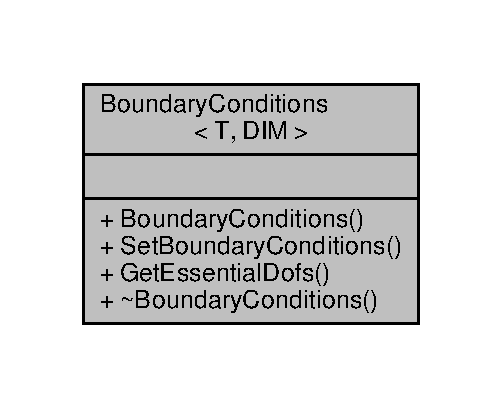
\includegraphics[width=241pt]{classBoundaryConditions__coll__graph}
\end{center}
\end{figure}
\subsection*{Public Member Functions}
\begin{DoxyCompactItemize}
\item 
{\footnotesize template$<$class... Args$>$ }\\\hyperlink{classBoundaryConditions_ae9bad35a04c1ef84eb7aa38425d6b044}{Boundary\+Conditions} (\hyperlink{classSpatialDiscretization}{Spatial\+Discretization}$<$ T, D\+IM $>$ $\ast$spatial, const Args \&...boundaries)
\begin{DoxyCompactList}\small\item\em Construct a new \hyperlink{classBoundary}{Boundary} Conditions\+:\+: \hyperlink{classBoundary}{Boundary} Conditions object. \end{DoxyCompactList}\item 
void \hyperlink{classBoundaryConditions_a23f5cf33a22290a61bb2dcba457f086d}{Set\+Boundary\+Conditions} (mfem\+::\+Vector \&u)
\begin{DoxyCompactList}\small\item\em Set boundary conditions. \end{DoxyCompactList}\item 
mfem\+::\+Array$<$ int $>$ \hyperlink{classBoundaryConditions_a3dcecb34a6ac7a00e6f110677145f7c8}{Get\+Essential\+Dofs} ()
\begin{DoxyCompactList}\small\item\em return the list of essential dofs \end{DoxyCompactList}\item 
\mbox{\Hypertarget{classBoundaryConditions_a50d3971dff965883752e17c05b468756}\label{classBoundaryConditions_a50d3971dff965883752e17c05b468756}} 
\hyperlink{classBoundaryConditions_a50d3971dff965883752e17c05b468756}{$\sim$\+Boundary\+Conditions} ()
\begin{DoxyCompactList}\small\item\em Destroy the \hyperlink{classBoundary}{Boundary} Conditions\+:\+: \hyperlink{classBoundary}{Boundary} Conditions object. \end{DoxyCompactList}\end{DoxyCompactItemize}


\subsection{Detailed Description}
\subsubsection*{template$<$class T, int D\+IM$>$\newline
class Boundary\+Conditions$<$ T, D\+I\+M $>$}

Class used to manage boundary conditions. 

Definition at line 25 of file Boundary\+Conditions.\+hpp.



\subsection{Constructor \& Destructor Documentation}
\mbox{\Hypertarget{classBoundaryConditions_ae9bad35a04c1ef84eb7aa38425d6b044}\label{classBoundaryConditions_ae9bad35a04c1ef84eb7aa38425d6b044}} 
\index{Boundary\+Conditions@{Boundary\+Conditions}!Boundary\+Conditions@{Boundary\+Conditions}}
\index{Boundary\+Conditions@{Boundary\+Conditions}!Boundary\+Conditions@{Boundary\+Conditions}}
\subsubsection{\texorpdfstring{Boundary\+Conditions()}{BoundaryConditions()}}
{\footnotesize\ttfamily template$<$class T , int D\+IM$>$ \\
template$<$class... Args$>$ \\
\hyperlink{classBoundaryConditions}{Boundary\+Conditions}$<$ T, D\+IM $>$\+::\hyperlink{classBoundaryConditions}{Boundary\+Conditions} (\begin{DoxyParamCaption}\item[{\hyperlink{classSpatialDiscretization}{Spatial\+Discretization}$<$ T, D\+IM $>$ $\ast$}]{spatial,  }\item[{const Args \&...}]{boundaries }\end{DoxyParamCaption})}



Construct a new \hyperlink{classBoundary}{Boundary} Conditions\+:\+: \hyperlink{classBoundary}{Boundary} Conditions object. 


\begin{DoxyTemplParams}{Template Parameters}
{\em Args} & \\
\hline
\end{DoxyTemplParams}

\begin{DoxyParams}{Parameters}
{\em fespace} & \\
\hline
{\em mesh\+\_\+max\+\_\+bdr\+\_\+attributes} & \\
\hline
{\em boundaries} & \\
\hline
\end{DoxyParams}


Definition at line 52 of file Boundary\+Conditions.\+hpp.



References Spatial\+Discretization$<$ T, D\+I\+M $>$\+::get\+\_\+finite\+\_\+element\+\_\+space(), and Spatial\+Discretization$<$ T, D\+I\+M $>$\+::get\+\_\+max\+\_\+bdr\+\_\+attributes().


\begin{DoxyCode}
53                                                                           \{
54   this->fespace\_ = spatial->\hyperlink{classSpatialDiscretization_ac001fc2ff356fe8c0c2b49618e594a03}{get\_finite\_element\_space}();
55   \textcolor{keyword}{const} \textcolor{keyword}{auto} &mesh\_max\_bdr\_attributes = spatial->\hyperlink{classSpatialDiscretization_aa6fe6ae45f18daf5a20fbc8b49b2ef05}{get\_max\_bdr\_attributes}();
56 
57   \textcolor{keyword}{auto} bdrs = std::vector<Boundary>\{boundaries...\};
58 
59   Dirichlet\_bdr\_.SetSize(mesh\_max\_bdr\_attributes);
60   Dirichlet\_value\_.SetSize(mesh\_max\_bdr\_attributes);
61   \textcolor{keywordtype}{bool} exist\_periodic\_bdr = \{\textcolor{keyword}{false}\};
62   [bdrs, &exist\_periodic\_bdr]() \{
63     \textcolor{keywordtype}{bool} is\_periodic = \textcolor{keyword}{false};
64     \textcolor{keywordflow}{for} (\textcolor{keyword}{const} \textcolor{keyword}{auto} &bdr : bdrs) \{
65       \textcolor{keywordflow}{if} (bdr.is\_essential\_boundary()) \{
66         is\_periodic = \textcolor{keyword}{true};
67         \textcolor{keywordflow}{break};
68       \}
69     \}
70     \textcolor{keywordflow}{return} is\_periodic;
71   \};
72   \textcolor{keywordtype}{bool} test\_periodic\_bdr = (mesh\_max\_bdr\_attributes != bdrs.size()) && exist\_periodic\_bdr;
73   \textcolor{keywordtype}{bool} test\_standard\_bdr = mesh\_max\_bdr\_attributes == bdrs.size();
74   \textcolor{keywordflow}{if} (test\_periodic\_bdr || test\_standard\_bdr) \{
75     \textcolor{keywordflow}{for} (\textcolor{keyword}{const} \textcolor{keyword}{auto} &bdr : bdrs) \{
76       \textcolor{keyword}{const} \textcolor{keyword}{auto} &\textcolor{keywordtype}{id} = bdr.get\_boundary\_index();
77       \textcolor{keywordflow}{if} (bdr.is\_essential\_boundary()) \{
78         Dirichlet\_bdr\_[id] = 1;
79       \} \textcolor{keywordflow}{else} \{
80         Dirichlet\_bdr\_[id] = 0;
81       \}
82       Dirichlet\_value\_[id] = bdr.get\_boundary\_value();
83     \}
84     this->fespace\_->GetEssentialTrueDofs(this->Dirichlet\_bdr\_, this->ess\_tdof\_list\_);
85   \} \textcolor{keywordflow}{else} \{
86     \textcolor{keywordflow}{throw} std::runtime\_error(
87         \textcolor{stringliteral}{"BoundaryConditions::BoundaryConditions(): user-defined boundaries  "} +
88         std::to\_string(bdrs.size()) +
89         \textcolor{stringliteral}{" are unconsistent with the total number of boundaries associated to the mesh "} +
90         std::to\_string(mesh\_max\_bdr\_attributes));
91   \}
92 \}
\end{DoxyCode}


\subsection{Member Function Documentation}
\mbox{\Hypertarget{classBoundaryConditions_a3dcecb34a6ac7a00e6f110677145f7c8}\label{classBoundaryConditions_a3dcecb34a6ac7a00e6f110677145f7c8}} 
\index{Boundary\+Conditions@{Boundary\+Conditions}!Get\+Essential\+Dofs@{Get\+Essential\+Dofs}}
\index{Get\+Essential\+Dofs@{Get\+Essential\+Dofs}!Boundary\+Conditions@{Boundary\+Conditions}}
\subsubsection{\texorpdfstring{Get\+Essential\+Dofs()}{GetEssentialDofs()}}
{\footnotesize\ttfamily template$<$class T , int D\+IM$>$ \\
mfem\+::\+Array$<$ int $>$ \hyperlink{classBoundaryConditions}{Boundary\+Conditions}$<$ T, D\+IM $>$\+::Get\+Essential\+Dofs (\begin{DoxyParamCaption}{ }\end{DoxyParamCaption})}



return the list of essential dofs 

\begin{DoxyReturn}{Returns}
mfem\+::\+Array$<$int$>$ array of essential dofs 
\end{DoxyReturn}


Definition at line 100 of file Boundary\+Conditions.\+hpp.



Referenced by Phase\+Field\+Operator\+Base$<$ T, D\+I\+M, N\+L\+F\+I $>$\+::initialize().


\begin{DoxyCode}
100                                                             \{
101   \textcolor{keywordflow}{return} this->ess\_tdof\_list\_;
102 \}
\end{DoxyCode}
\mbox{\Hypertarget{classBoundaryConditions_a23f5cf33a22290a61bb2dcba457f086d}\label{classBoundaryConditions_a23f5cf33a22290a61bb2dcba457f086d}} 
\index{Boundary\+Conditions@{Boundary\+Conditions}!Set\+Boundary\+Conditions@{Set\+Boundary\+Conditions}}
\index{Set\+Boundary\+Conditions@{Set\+Boundary\+Conditions}!Boundary\+Conditions@{Boundary\+Conditions}}
\subsubsection{\texorpdfstring{Set\+Boundary\+Conditions()}{SetBoundaryConditions()}}
{\footnotesize\ttfamily template$<$class T , int D\+IM$>$ \\
void \hyperlink{classBoundaryConditions}{Boundary\+Conditions}$<$ T, D\+IM $>$\+::Set\+Boundary\+Conditions (\begin{DoxyParamCaption}\item[{mfem\+::\+Vector \&}]{u }\end{DoxyParamCaption})}



Set boundary conditions. 


\begin{DoxyParams}{Parameters}
{\em u} & unknown vector \\
\hline
\end{DoxyParams}


Definition at line 110 of file Boundary\+Conditions.\+hpp.



Referenced by Phase\+Field\+Operator\+Base$<$ T, D\+I\+M, N\+L\+F\+I $>$\+::\+Implicit\+Solve(), and Phase\+Field\+Operator\+Base$<$ T, D\+I\+M, N\+L\+F\+I $>$\+::initialize().


\begin{DoxyCode}
110                                                                     \{
111   mfem::Array<int> tmp\_array\_bdr(this->Dirichlet\_bdr\_.Size());
112   \textcolor{keywordflow}{for} (\textcolor{keyword}{auto} i = 0; i < this->Dirichlet\_bdr\_.Size(); i++) \{
113     tmp\_array\_bdr = 0;
114     mfem::Array<int> dof;
115     \textcolor{keywordflow}{if} (this->Dirichlet\_bdr\_[i] > 0) \{
116       tmp\_array\_bdr[i] = 1;
117       this->fespace\_->GetEssentialTrueDofs(tmp\_array\_bdr, dof);
118       u.SetSubVector(dof, this->Dirichlet\_value\_[i]);
119     \}
120   \}
121 \}  \textcolor{comment}{// end of SetBoundaryConditions}
\end{DoxyCode}


The documentation for this class was generated from the following file\+:\begin{DoxyCompactItemize}
\item 
Boundary\+Conditions.\+hpp\end{DoxyCompactItemize}

\hypertarget{structBoundaryConditionType}{}\section{Boundary\+Condition\+Type Struct Reference}
\label{structBoundaryConditionType}\index{Boundary\+Condition\+Type@{Boundary\+Condition\+Type}}


Collaboration diagram for Boundary\+Condition\+Type\+:\nopagebreak
\begin{figure}[H]
\begin{center}
\leavevmode
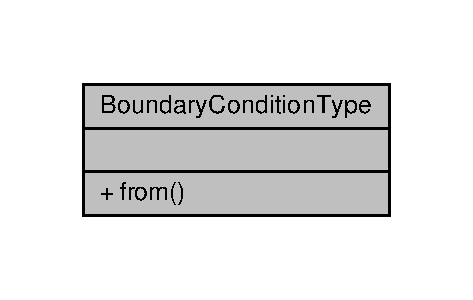
\includegraphics[width=227pt]{structBoundaryConditionType__coll__graph}
\end{center}
\end{figure}
\subsection*{Public Types}
\begin{DoxyCompactItemize}
\item 
\mbox{\Hypertarget{structBoundaryConditionType_a3571a0166b96db9c4322ec66fb76c254}\label{structBoundaryConditionType_a3571a0166b96db9c4322ec66fb76c254}} 
enum {\bfseries value} \{ {\bfseries Dirichlet}, 
{\bfseries Neumann}, 
{\bfseries Periodic}, 
{\bfseries Robin}
 \}
\end{DoxyCompactItemize}
\subsection*{Static Public Member Functions}
\begin{DoxyCompactItemize}
\item 
\mbox{\Hypertarget{structBoundaryConditionType_abd1f82993a717a61249de91d2cff67e4}\label{structBoundaryConditionType_abd1f82993a717a61249de91d2cff67e4}} 
static value {\bfseries from} (const std\+::string \&)
\end{DoxyCompactItemize}


\subsection{Detailed Description}


Definition at line 110 of file Utils/\+Phase\+Field\+Options.\+hpp.



The documentation for this struct was generated from the following file\+:\begin{DoxyCompactItemize}
\item 
Utils/\+Phase\+Field\+Options.\+hpp\end{DoxyCompactItemize}

\hypertarget{classConductionOperator}{}\section{Conduction\+Operator Class Reference}
\label{classConductionOperator}\index{Conduction\+Operator@{Conduction\+Operator}}


Inheritance diagram for Conduction\+Operator\+:\nopagebreak
\begin{figure}[H]
\begin{center}
\leavevmode
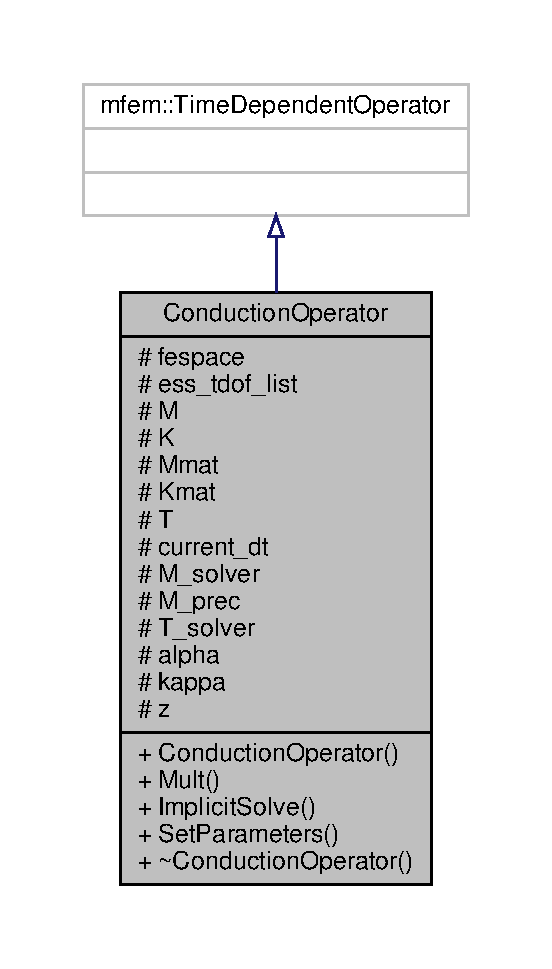
\includegraphics[width=265pt]{classConductionOperator__inherit__graph}
\end{center}
\end{figure}


Collaboration diagram for Conduction\+Operator\+:\nopagebreak
\begin{figure}[H]
\begin{center}
\leavevmode
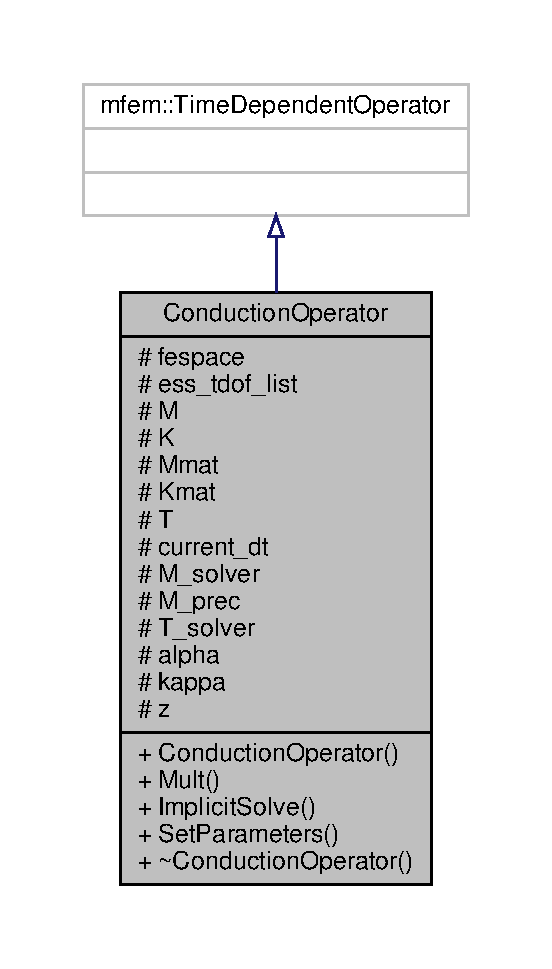
\includegraphics[width=265pt]{classConductionOperator__coll__graph}
\end{center}
\end{figure}
\subsection*{Public Member Functions}
\begin{DoxyCompactItemize}
\item 
\mbox{\Hypertarget{classConductionOperator_a015df11ae1f4e77b73f0e22a5f3984fb}\label{classConductionOperator_a015df11ae1f4e77b73f0e22a5f3984fb}} 
{\bfseries Conduction\+Operator} (mfem\+::\+Finite\+Element\+Space \&f, double alpha, double kappa, mfem\+::\+Vector \&u)
\item 
\mbox{\Hypertarget{classConductionOperator_a2b6fa0ab4288598d53cf324fa3120b3f}\label{classConductionOperator_a2b6fa0ab4288598d53cf324fa3120b3f}} 
virtual void {\bfseries Mult} (const mfem\+::\+Vector \&u, mfem\+::\+Vector \&du\+\_\+dt) const
\item 
virtual void \hyperlink{classConductionOperator_a4bffd1dac813fdaf47a3e6d558e73076}{Implicit\+Solve} (const double dt, const mfem\+::\+Vector \&u, mfem\+::\+Vector \&k)
\item 
\mbox{\Hypertarget{classConductionOperator_ae8ee86b31f6e5ff3290ad59e1a9dba6c}\label{classConductionOperator_ae8ee86b31f6e5ff3290ad59e1a9dba6c}} 
void \hyperlink{classConductionOperator_ae8ee86b31f6e5ff3290ad59e1a9dba6c}{Set\+Parameters} (const mfem\+::\+Vector \&u)
\begin{DoxyCompactList}\small\item\em Update the diffusion Bilinear\+Form K using the given true-\/dof vector {\ttfamily u}. \end{DoxyCompactList}\end{DoxyCompactItemize}
\subsection*{Protected Attributes}
\begin{DoxyCompactItemize}
\item 
\mbox{\Hypertarget{classConductionOperator_a49b42a0db05029f9961d0d23a1979e2a}\label{classConductionOperator_a49b42a0db05029f9961d0d23a1979e2a}} 
mfem\+::\+Finite\+Element\+Space \& {\bfseries fespace}
\item 
\mbox{\Hypertarget{classConductionOperator_a521f3698e5702df96bbd6f1f5f8d7066}\label{classConductionOperator_a521f3698e5702df96bbd6f1f5f8d7066}} 
mfem\+::\+Array$<$ int $>$ {\bfseries ess\+\_\+tdof\+\_\+list}
\item 
\mbox{\Hypertarget{classConductionOperator_a3c448eca1db50893bfd044d18841e4d6}\label{classConductionOperator_a3c448eca1db50893bfd044d18841e4d6}} 
mfem\+::\+Bilinear\+Form $\ast$ {\bfseries M}
\item 
\mbox{\Hypertarget{classConductionOperator_aa5f7b920a14eed6b70c105e7dc111392}\label{classConductionOperator_aa5f7b920a14eed6b70c105e7dc111392}} 
mfem\+::\+Bilinear\+Form $\ast$ {\bfseries K}
\item 
\mbox{\Hypertarget{classConductionOperator_a36f4dcda0997c9a276ef1c5a75785a50}\label{classConductionOperator_a36f4dcda0997c9a276ef1c5a75785a50}} 
mfem\+::\+Sparse\+Matrix {\bfseries Mmat}
\item 
\mbox{\Hypertarget{classConductionOperator_ab293e6ed42f25a8b80473e972bb52c65}\label{classConductionOperator_ab293e6ed42f25a8b80473e972bb52c65}} 
mfem\+::\+Sparse\+Matrix {\bfseries Kmat}
\item 
\mbox{\Hypertarget{classConductionOperator_a5f82c75ed63e12a5854c290b8aa78e35}\label{classConductionOperator_a5f82c75ed63e12a5854c290b8aa78e35}} 
mfem\+::\+Sparse\+Matrix $\ast$ {\bfseries T}
\item 
\mbox{\Hypertarget{classConductionOperator_a74cef1ccf53e9ea7692d9969cfb5ac4f}\label{classConductionOperator_a74cef1ccf53e9ea7692d9969cfb5ac4f}} 
double {\bfseries current\+\_\+dt}
\item 
\mbox{\Hypertarget{classConductionOperator_a50ce90a6225abb165253b27969cc2e76}\label{classConductionOperator_a50ce90a6225abb165253b27969cc2e76}} 
mfem\+::\+C\+G\+Solver {\bfseries M\+\_\+solver}
\item 
\mbox{\Hypertarget{classConductionOperator_ab1a44c70228ed5a061facc240f85eded}\label{classConductionOperator_ab1a44c70228ed5a061facc240f85eded}} 
mfem\+::\+D\+Smoother {\bfseries M\+\_\+prec}
\item 
\mbox{\Hypertarget{classConductionOperator_a645ee0cb582c7b25eb8ee39922a39ca5}\label{classConductionOperator_a645ee0cb582c7b25eb8ee39922a39ca5}} 
mfem\+::\+U\+M\+F\+Pack\+Solver {\bfseries T\+\_\+solver}
\item 
\mbox{\Hypertarget{classConductionOperator_ae5aaf625475e983cf93100c16b6c285e}\label{classConductionOperator_ae5aaf625475e983cf93100c16b6c285e}} 
double {\bfseries alpha}
\item 
\mbox{\Hypertarget{classConductionOperator_aec2ae48d7ba52364cd65edebf456322c}\label{classConductionOperator_aec2ae48d7ba52364cd65edebf456322c}} 
double {\bfseries kappa}
\item 
\mbox{\Hypertarget{classConductionOperator_a3d65a4324d9f6ebb18dd654ce640872c}\label{classConductionOperator_a3d65a4324d9f6ebb18dd654ce640872c}} 
mfem\+::\+Vector {\bfseries z}
\end{DoxyCompactItemize}


\subsection{Detailed Description}


Definition at line 19 of file Conduction\+Operator.\+hpp.



\subsection{Member Function Documentation}
\mbox{\Hypertarget{classConductionOperator_a4bffd1dac813fdaf47a3e6d558e73076}\label{classConductionOperator_a4bffd1dac813fdaf47a3e6d558e73076}} 
\index{Conduction\+Operator@{Conduction\+Operator}!Implicit\+Solve@{Implicit\+Solve}}
\index{Implicit\+Solve@{Implicit\+Solve}!Conduction\+Operator@{Conduction\+Operator}}
\subsubsection{\texorpdfstring{Implicit\+Solve()}{ImplicitSolve()}}
{\footnotesize\ttfamily void Conduction\+Operator\+::\+Implicit\+Solve (\begin{DoxyParamCaption}\item[{const double}]{dt,  }\item[{const mfem\+::\+Vector \&}]{u,  }\item[{mfem\+::\+Vector \&}]{k }\end{DoxyParamCaption})\hspace{0.3cm}{\ttfamily [virtual]}}

Solve the Backward-\/\+Euler equation\+: k = f(u + dt$\ast$k, t), for the unknown k. This is the only requirement for high-\/order S\+D\+I\+RK implicit integration. 

Definition at line 137 of file Conduction\+Operator.\+hpp.


\begin{DoxyCode}
138                                                           \{
139   \textcolor{comment}{// Solve the equation:}
140   \textcolor{comment}{//    du\_dt = M^\{-1\}*[-K(u + dt*du\_dt)]}
141   \textcolor{comment}{// for du\_dt, where K is linearized by using u from the previous timestep}
142   \textcolor{keywordflow}{if} (!T) \{
143     T = Add(1.0, Mmat, dt, Kmat);
144     current\_dt = dt;
145     T\_solver.SetOperator(*T);
146   \}
147   MFEM\_VERIFY(dt == current\_dt, \textcolor{stringliteral}{""});  \textcolor{comment}{// SDIRK methods use the same dt}
148   Kmat.Mult(u, z);
149   z.Neg();
150 
151   T\_solver.Mult(z, du\_dt);
152   du\_dt.SetSubVector(ess\_tdof\_list, 0.0);
153 \}
\end{DoxyCode}


The documentation for this class was generated from the following file\+:\begin{DoxyCompactItemize}
\item 
Conduction\+Operator.\+hpp\end{DoxyCompactItemize}

\hypertarget{classDiffusionNLFIntegrator}{}\section{Diffusion\+N\+L\+F\+Integrator Class Reference}
\label{classDiffusionNLFIntegrator}\index{Diffusion\+N\+L\+F\+Integrator@{Diffusion\+N\+L\+F\+Integrator}}


Inheritance diagram for Diffusion\+N\+L\+F\+Integrator\+:\nopagebreak
\begin{figure}[H]
\begin{center}
\leavevmode
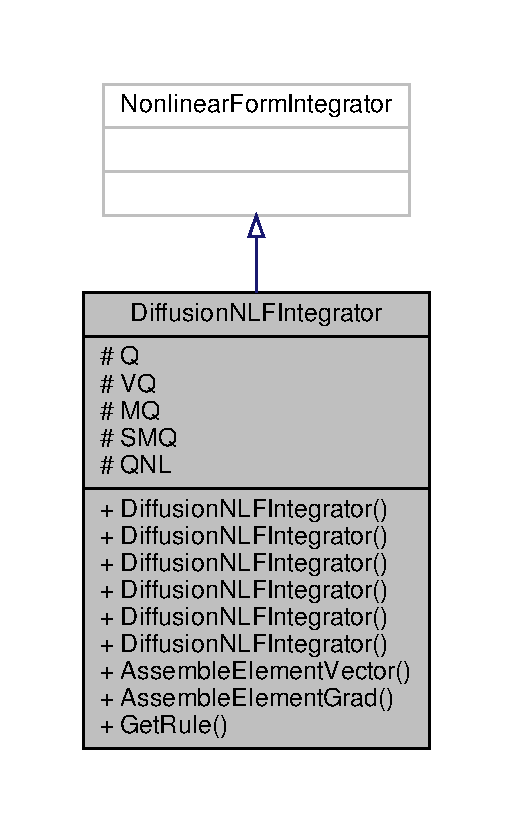
\includegraphics[width=246pt]{classDiffusionNLFIntegrator__inherit__graph}
\end{center}
\end{figure}


Collaboration diagram for Diffusion\+N\+L\+F\+Integrator\+:\nopagebreak
\begin{figure}[H]
\begin{center}
\leavevmode
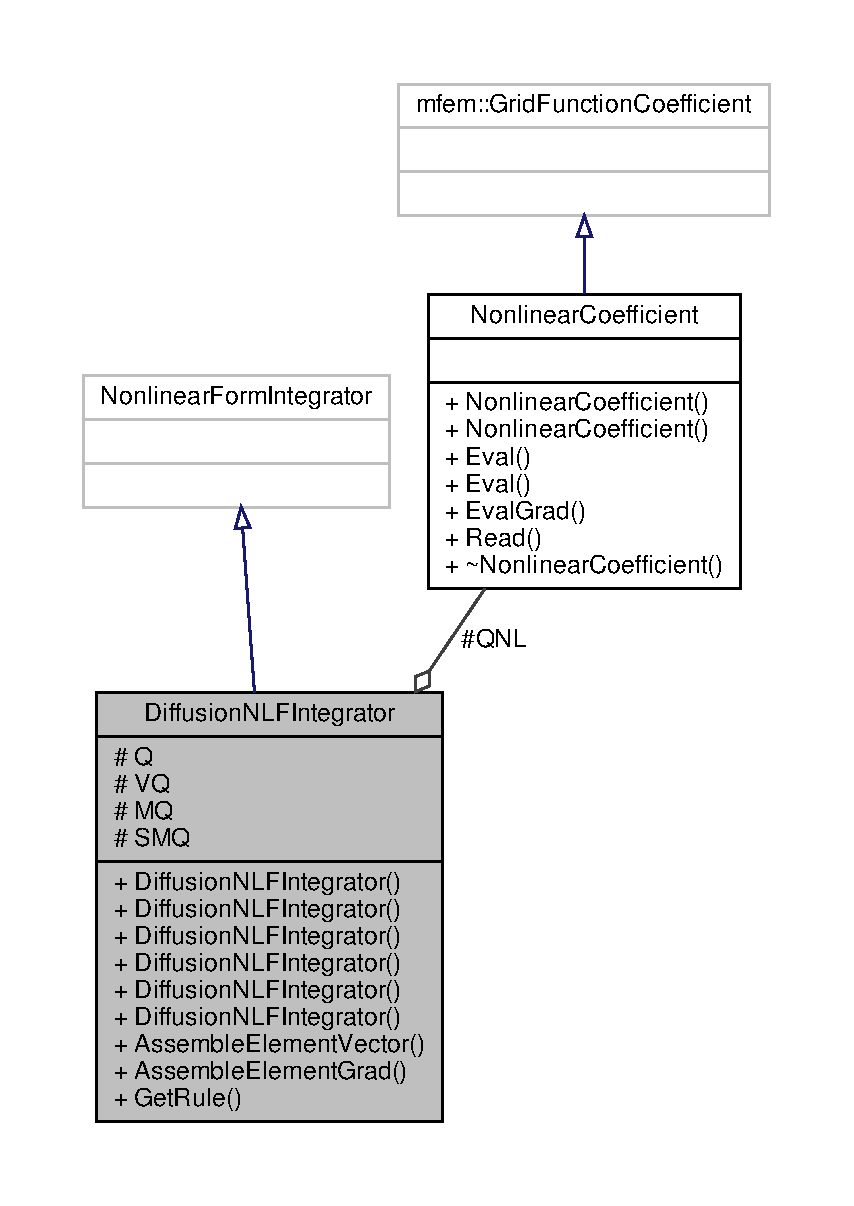
\includegraphics[width=350pt]{classDiffusionNLFIntegrator__coll__graph}
\end{center}
\end{figure}
\subsection*{Public Member Functions}
\begin{DoxyCompactItemize}
\item 
\mbox{\Hypertarget{classDiffusionNLFIntegrator_aa5ac1c68c41c380ae93cae393f7d6f58}\label{classDiffusionNLFIntegrator_aa5ac1c68c41c380ae93cae393f7d6f58}} 
\hyperlink{classDiffusionNLFIntegrator_aa5ac1c68c41c380ae93cae393f7d6f58}{Diffusion\+N\+L\+F\+Integrator} ()
\begin{DoxyCompactList}\small\item\em Construct a diffusion nonliner integrator with coefficient Q = 1. \end{DoxyCompactList}\item 
\hyperlink{classDiffusionNLFIntegrator_afca901531276e09a8422f49feb21f8e8}{Diffusion\+N\+L\+F\+Integrator} (mfem\+::\+Constant\+Coefficient \&q)
\item 
\hyperlink{classDiffusionNLFIntegrator_ab36835fb8a4338e17d34e06fb78eefdb}{Diffusion\+N\+L\+F\+Integrator} (mfem\+::\+Constant\+Coefficient \&q, \hyperlink{classNonlinearCoefficient}{Nonlinear\+Coefficient} \&qq)
\item 
\hyperlink{classDiffusionNLFIntegrator_a8ac2d40eeb337b5e583af9aa507b3f79}{Diffusion\+N\+L\+F\+Integrator} (mfem\+::\+Vector\+Coefficient \&q, \hyperlink{classNonlinearCoefficient}{Nonlinear\+Coefficient} \&qq)
\item 
\hyperlink{classDiffusionNLFIntegrator_a12fc3a8e2a499ca7751d570df106bcf3}{Diffusion\+N\+L\+F\+Integrator} (mfem\+::\+Matrix\+Coefficient \&q, \hyperlink{classNonlinearCoefficient}{Nonlinear\+Coefficient} \&qq)
\item 
\hyperlink{classDiffusionNLFIntegrator_adcfdeb40ded7183d014271e67dd767b5}{Diffusion\+N\+L\+F\+Integrator} (mfem\+::\+Symmetric\+Matrix\+Coefficient \&q, \hyperlink{classNonlinearCoefficient}{Nonlinear\+Coefficient} \&qq)
\item 
\mbox{\Hypertarget{classDiffusionNLFIntegrator_acce6dfc2efb977559c9dcc75f12dcb22}\label{classDiffusionNLFIntegrator_acce6dfc2efb977559c9dcc75f12dcb22}} 
virtual void \hyperlink{classDiffusionNLFIntegrator_acce6dfc2efb977559c9dcc75f12dcb22}{Assemble\+Element\+Vector} (const mfem\+::\+Finite\+Element \&el, mfem\+::\+Element\+Transformation \&Tr, const mfem\+::\+Vector \&elfun, mfem\+::\+Vector \&elvect)
\begin{DoxyCompactList}\small\item\em Given a elfun values perform the local action of the Nonlinear\+Form\+Integrator. \end{DoxyCompactList}\item 
\mbox{\Hypertarget{classDiffusionNLFIntegrator_ac7b70b5cee3c880d52b03a87706ae8e3}\label{classDiffusionNLFIntegrator_ac7b70b5cee3c880d52b03a87706ae8e3}} 
virtual void \hyperlink{classDiffusionNLFIntegrator_ac7b70b5cee3c880d52b03a87706ae8e3}{Assemble\+Element\+Grad} (const mfem\+::\+Finite\+Element \&el, mfem\+::\+Element\+Transformation \&Tr, const mfem\+::\+Vector \&elfun, mfem\+::\+Dense\+Matrix \&elmat)
\begin{DoxyCompactList}\small\item\em Assemble the local gradient matrix. \end{DoxyCompactList}\end{DoxyCompactItemize}
\subsection*{Static Public Member Functions}
\begin{DoxyCompactItemize}
\item 
\mbox{\Hypertarget{classDiffusionNLFIntegrator_a5edf482fa4fc51004636c7f21624c189}\label{classDiffusionNLFIntegrator_a5edf482fa4fc51004636c7f21624c189}} 
static const mfem\+::\+Integration\+Rule \& {\bfseries Get\+Rule} (const mfem\+::\+Finite\+Element \&fe, mfem\+::\+Element\+Transformation \&T)
\end{DoxyCompactItemize}
\subsection*{Protected Attributes}
\begin{DoxyCompactItemize}
\item 
\mbox{\Hypertarget{classDiffusionNLFIntegrator_a6c7536d247373af0bda2079c2440fe7f}\label{classDiffusionNLFIntegrator_a6c7536d247373af0bda2079c2440fe7f}} 
mfem\+::\+Constant\+Coefficient $\ast$ {\bfseries Q}
\item 
\mbox{\Hypertarget{classDiffusionNLFIntegrator_af061475fcd1cd075e25272501e47477e}\label{classDiffusionNLFIntegrator_af061475fcd1cd075e25272501e47477e}} 
mfem\+::\+Vector\+Coefficient $\ast$ {\bfseries VQ}
\item 
\mbox{\Hypertarget{classDiffusionNLFIntegrator_a50df2e3961e28929d51ea565f954a6d5}\label{classDiffusionNLFIntegrator_a50df2e3961e28929d51ea565f954a6d5}} 
mfem\+::\+Matrix\+Coefficient $\ast$ {\bfseries MQ}
\item 
\mbox{\Hypertarget{classDiffusionNLFIntegrator_a37a89ee4999577e96733d3f1a5522896}\label{classDiffusionNLFIntegrator_a37a89ee4999577e96733d3f1a5522896}} 
mfem\+::\+Symmetric\+Matrix\+Coefficient $\ast$ {\bfseries S\+MQ}
\item 
\mbox{\Hypertarget{classDiffusionNLFIntegrator_a69764c9ab0bc5424a1a4730a034d28cb}\label{classDiffusionNLFIntegrator_a69764c9ab0bc5424a1a4730a034d28cb}} 
\hyperlink{classNonlinearCoefficient}{Nonlinear\+Coefficient} $\ast$ {\bfseries Q\+NL}
\end{DoxyCompactItemize}


\subsection{Detailed Description}


Definition at line 48 of file Diffusion\+N\+L\+F\+Integrator.\+hpp.



\subsection{Constructor \& Destructor Documentation}
\mbox{\Hypertarget{classDiffusionNLFIntegrator_afca901531276e09a8422f49feb21f8e8}\label{classDiffusionNLFIntegrator_afca901531276e09a8422f49feb21f8e8}} 
\index{Diffusion\+N\+L\+F\+Integrator@{Diffusion\+N\+L\+F\+Integrator}!Diffusion\+N\+L\+F\+Integrator@{Diffusion\+N\+L\+F\+Integrator}}
\index{Diffusion\+N\+L\+F\+Integrator@{Diffusion\+N\+L\+F\+Integrator}!Diffusion\+N\+L\+F\+Integrator@{Diffusion\+N\+L\+F\+Integrator}}
\subsubsection{\texorpdfstring{Diffusion\+N\+L\+F\+Integrator()}{DiffusionNLFIntegrator()}\hspace{0.1cm}{\footnotesize\ttfamily [1/5]}}
{\footnotesize\ttfamily Diffusion\+N\+L\+F\+Integrator\+::\+Diffusion\+N\+L\+F\+Integrator (\begin{DoxyParamCaption}\item[{mfem\+::\+Constant\+Coefficient \&}]{q }\end{DoxyParamCaption})\hspace{0.3cm}{\ttfamily [inline]}}

Construct a diffusion integrator with a scalar coefficient q and nonlinear coefficient qq 

Definition at line 69 of file Diffusion\+N\+L\+F\+Integrator.\+hpp.


\begin{DoxyCode}
70       : Q(&q), VQ(NULL), MQ(NULL), SMQ(NULL), QNL(NULL) \{\}
\end{DoxyCode}
\mbox{\Hypertarget{classDiffusionNLFIntegrator_ab36835fb8a4338e17d34e06fb78eefdb}\label{classDiffusionNLFIntegrator_ab36835fb8a4338e17d34e06fb78eefdb}} 
\index{Diffusion\+N\+L\+F\+Integrator@{Diffusion\+N\+L\+F\+Integrator}!Diffusion\+N\+L\+F\+Integrator@{Diffusion\+N\+L\+F\+Integrator}}
\index{Diffusion\+N\+L\+F\+Integrator@{Diffusion\+N\+L\+F\+Integrator}!Diffusion\+N\+L\+F\+Integrator@{Diffusion\+N\+L\+F\+Integrator}}
\subsubsection{\texorpdfstring{Diffusion\+N\+L\+F\+Integrator()}{DiffusionNLFIntegrator()}\hspace{0.1cm}{\footnotesize\ttfamily [2/5]}}
{\footnotesize\ttfamily Diffusion\+N\+L\+F\+Integrator\+::\+Diffusion\+N\+L\+F\+Integrator (\begin{DoxyParamCaption}\item[{mfem\+::\+Constant\+Coefficient \&}]{q,  }\item[{\hyperlink{classNonlinearCoefficient}{Nonlinear\+Coefficient} \&}]{qq }\end{DoxyParamCaption})\hspace{0.3cm}{\ttfamily [inline]}}

Construct a diffusion integrator with a scalar coefficient q and nonlinear coefficient qq 

Definition at line 74 of file Diffusion\+N\+L\+F\+Integrator.\+hpp.


\begin{DoxyCode}
75       : Q(&q), VQ(NULL), MQ(NULL), SMQ(NULL), QNL(&qq) \{\}
\end{DoxyCode}
\mbox{\Hypertarget{classDiffusionNLFIntegrator_a8ac2d40eeb337b5e583af9aa507b3f79}\label{classDiffusionNLFIntegrator_a8ac2d40eeb337b5e583af9aa507b3f79}} 
\index{Diffusion\+N\+L\+F\+Integrator@{Diffusion\+N\+L\+F\+Integrator}!Diffusion\+N\+L\+F\+Integrator@{Diffusion\+N\+L\+F\+Integrator}}
\index{Diffusion\+N\+L\+F\+Integrator@{Diffusion\+N\+L\+F\+Integrator}!Diffusion\+N\+L\+F\+Integrator@{Diffusion\+N\+L\+F\+Integrator}}
\subsubsection{\texorpdfstring{Diffusion\+N\+L\+F\+Integrator()}{DiffusionNLFIntegrator()}\hspace{0.1cm}{\footnotesize\ttfamily [3/5]}}
{\footnotesize\ttfamily Diffusion\+N\+L\+F\+Integrator\+::\+Diffusion\+N\+L\+F\+Integrator (\begin{DoxyParamCaption}\item[{mfem\+::\+Vector\+Coefficient \&}]{q,  }\item[{\hyperlink{classNonlinearCoefficient}{Nonlinear\+Coefficient} \&}]{qq }\end{DoxyParamCaption})\hspace{0.3cm}{\ttfamily [inline]}}

Construct a diffusion integrator with a vector coefficient q and nonlinear coefficient qq 

Definition at line 79 of file Diffusion\+N\+L\+F\+Integrator.\+hpp.


\begin{DoxyCode}
80       : Q(NULL), VQ(&q), MQ(NULL), SMQ(NULL), QNL(&qq) \{\}
\end{DoxyCode}
\mbox{\Hypertarget{classDiffusionNLFIntegrator_a12fc3a8e2a499ca7751d570df106bcf3}\label{classDiffusionNLFIntegrator_a12fc3a8e2a499ca7751d570df106bcf3}} 
\index{Diffusion\+N\+L\+F\+Integrator@{Diffusion\+N\+L\+F\+Integrator}!Diffusion\+N\+L\+F\+Integrator@{Diffusion\+N\+L\+F\+Integrator}}
\index{Diffusion\+N\+L\+F\+Integrator@{Diffusion\+N\+L\+F\+Integrator}!Diffusion\+N\+L\+F\+Integrator@{Diffusion\+N\+L\+F\+Integrator}}
\subsubsection{\texorpdfstring{Diffusion\+N\+L\+F\+Integrator()}{DiffusionNLFIntegrator()}\hspace{0.1cm}{\footnotesize\ttfamily [4/5]}}
{\footnotesize\ttfamily Diffusion\+N\+L\+F\+Integrator\+::\+Diffusion\+N\+L\+F\+Integrator (\begin{DoxyParamCaption}\item[{mfem\+::\+Matrix\+Coefficient \&}]{q,  }\item[{\hyperlink{classNonlinearCoefficient}{Nonlinear\+Coefficient} \&}]{qq }\end{DoxyParamCaption})\hspace{0.3cm}{\ttfamily [inline]}}

Construct a diffusion integrator with a matrix coefficient q and nonlinear coefficient qq 

Definition at line 84 of file Diffusion\+N\+L\+F\+Integrator.\+hpp.


\begin{DoxyCode}
85       : Q(NULL), VQ(NULL), MQ(&q), SMQ(NULL), QNL(&qq) \{\}
\end{DoxyCode}
\mbox{\Hypertarget{classDiffusionNLFIntegrator_adcfdeb40ded7183d014271e67dd767b5}\label{classDiffusionNLFIntegrator_adcfdeb40ded7183d014271e67dd767b5}} 
\index{Diffusion\+N\+L\+F\+Integrator@{Diffusion\+N\+L\+F\+Integrator}!Diffusion\+N\+L\+F\+Integrator@{Diffusion\+N\+L\+F\+Integrator}}
\index{Diffusion\+N\+L\+F\+Integrator@{Diffusion\+N\+L\+F\+Integrator}!Diffusion\+N\+L\+F\+Integrator@{Diffusion\+N\+L\+F\+Integrator}}
\subsubsection{\texorpdfstring{Diffusion\+N\+L\+F\+Integrator()}{DiffusionNLFIntegrator()}\hspace{0.1cm}{\footnotesize\ttfamily [5/5]}}
{\footnotesize\ttfamily Diffusion\+N\+L\+F\+Integrator\+::\+Diffusion\+N\+L\+F\+Integrator (\begin{DoxyParamCaption}\item[{mfem\+::\+Symmetric\+Matrix\+Coefficient \&}]{q,  }\item[{\hyperlink{classNonlinearCoefficient}{Nonlinear\+Coefficient} \&}]{qq }\end{DoxyParamCaption})\hspace{0.3cm}{\ttfamily [inline]}}

Construct a diffusion integrator with a symmetric matrix coefficient q and nonlinear coefficient qq 

Definition at line 89 of file Diffusion\+N\+L\+F\+Integrator.\+hpp.


\begin{DoxyCode}
90       : Q(NULL), VQ(NULL), MQ(NULL), SMQ(&q), QNL(&qq) \{\}
\end{DoxyCode}


The documentation for this class was generated from the following file\+:\begin{DoxyCompactItemize}
\item 
Diffusion\+N\+L\+F\+Integrator.\+hpp\end{DoxyCompactItemize}

\hypertarget{classEnergyCoefficient}{}\section{Energy\+Coefficient Class Reference}
\label{classEnergyCoefficient}\index{Energy\+Coefficient@{Energy\+Coefficient}}


Inheritance diagram for Energy\+Coefficient\+:\nopagebreak
\begin{figure}[H]
\begin{center}
\leavevmode
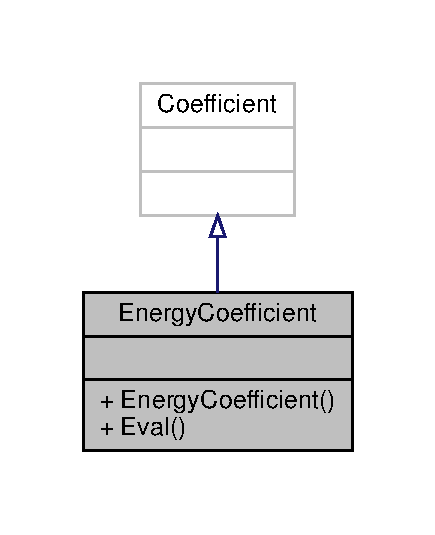
\includegraphics[width=209pt]{classEnergyCoefficient__inherit__graph}
\end{center}
\end{figure}


Collaboration diagram for Energy\+Coefficient\+:\nopagebreak
\begin{figure}[H]
\begin{center}
\leavevmode
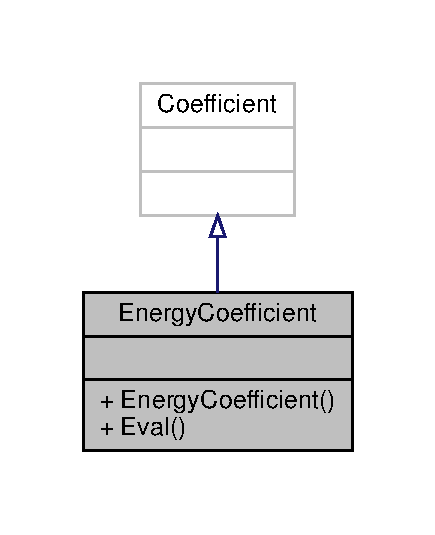
\includegraphics[width=209pt]{classEnergyCoefficient__coll__graph}
\end{center}
\end{figure}
\subsection*{Public Member Functions}
\begin{DoxyCompactItemize}
\item 
\mbox{\Hypertarget{classEnergyCoefficient_a9d94b692ae62d84664e5179e6af3ffb9}\label{classEnergyCoefficient_a9d94b692ae62d84664e5179e6af3ffb9}} 
{\bfseries Energy\+Coefficient} (mfem\+::\+Grid\+Function $\ast$gfu\+\_\+, const double \&lambda\+\_\+, const double \&omega\+\_\+)
\item 
\mbox{\Hypertarget{classEnergyCoefficient_a8d6c9fea967716a0252a047af09dfa21}\label{classEnergyCoefficient_a8d6c9fea967716a0252a047af09dfa21}} 
double {\bfseries Eval} (mfem\+::\+Element\+Transformation \&T, const mfem\+::\+Integration\+Point \&ip)
\end{DoxyCompactItemize}


\subsection{Detailed Description}


Definition at line 38 of file Energy\+Coefficient.\+hpp.



The documentation for this class was generated from the following file\+:\begin{DoxyCompactItemize}
\item 
Energy\+Coefficient.\+hpp\end{DoxyCompactItemize}

\hypertarget{classInterfacialCoefficient}{}\section{Interfacial\+Coefficient Class Reference}
\label{classInterfacialCoefficient}\index{Interfacial\+Coefficient@{Interfacial\+Coefficient}}


Inheritance diagram for Interfacial\+Coefficient\+:\nopagebreak
\begin{figure}[H]
\begin{center}
\leavevmode
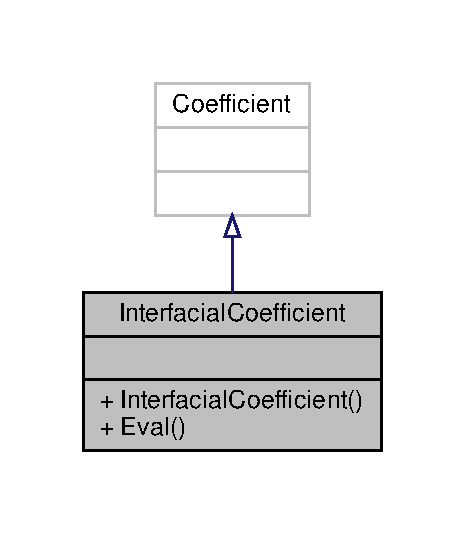
\includegraphics[width=223pt]{classInterfacialCoefficient__inherit__graph}
\end{center}
\end{figure}


Collaboration diagram for Interfacial\+Coefficient\+:\nopagebreak
\begin{figure}[H]
\begin{center}
\leavevmode
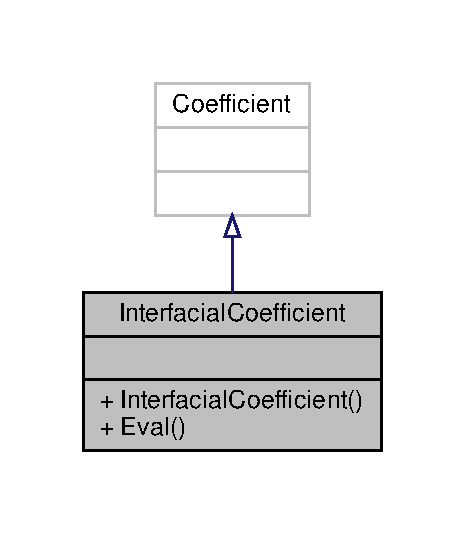
\includegraphics[width=223pt]{classInterfacialCoefficient__coll__graph}
\end{center}
\end{figure}
\subsection*{Public Member Functions}
\begin{DoxyCompactItemize}
\item 
\mbox{\Hypertarget{classInterfacialCoefficient_a97a4e4c020492eb889fd150aef6f4484}\label{classInterfacialCoefficient_a97a4e4c020492eb889fd150aef6f4484}} 
{\bfseries Interfacial\+Coefficient} (mfem\+::\+Grid\+Function $\ast$gfu\+\_\+, const double \&lambda\+\_\+)
\item 
\mbox{\Hypertarget{classInterfacialCoefficient_a129723114096b83dd145c6bea5ca83a4}\label{classInterfacialCoefficient_a129723114096b83dd145c6bea5ca83a4}} 
double {\bfseries Eval} (mfem\+::\+Element\+Transformation \&T, const mfem\+::\+Integration\+Point \&ip)
\end{DoxyCompactItemize}


\subsection{Detailed Description}


Definition at line 16 of file Energy\+Coefficient.\+hpp.



The documentation for this class was generated from the following file\+:\begin{DoxyCompactItemize}
\item 
Energy\+Coefficient.\+hpp\end{DoxyCompactItemize}

\hypertarget{classMeltingCoefficient}{}\section{Melting\+Coefficient Class Reference}
\label{classMeltingCoefficient}\index{Melting\+Coefficient@{Melting\+Coefficient}}


Inheritance diagram for Melting\+Coefficient\+:\nopagebreak
\begin{figure}[H]
\begin{center}
\leavevmode
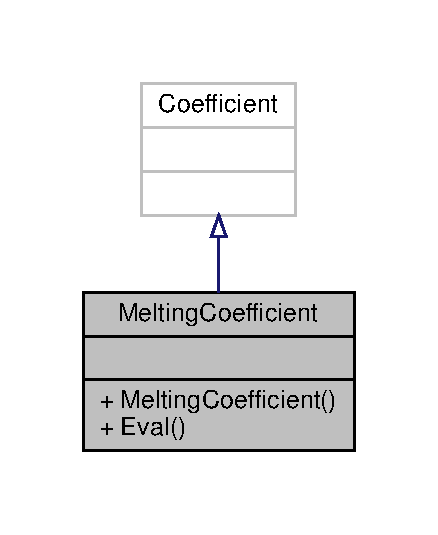
\includegraphics[width=210pt]{classMeltingCoefficient__inherit__graph}
\end{center}
\end{figure}


Collaboration diagram for Melting\+Coefficient\+:\nopagebreak
\begin{figure}[H]
\begin{center}
\leavevmode
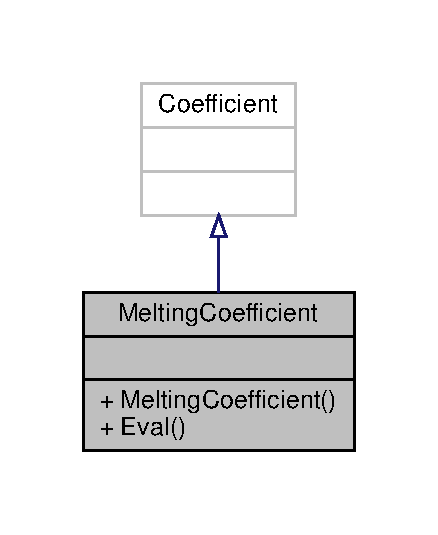
\includegraphics[width=210pt]{classMeltingCoefficient__coll__graph}
\end{center}
\end{figure}
\subsection*{Public Member Functions}
\begin{DoxyCompactItemize}
\item 
\mbox{\Hypertarget{classMeltingCoefficient_a670c052e07ed8e87af96cd29e619424c}\label{classMeltingCoefficient_a670c052e07ed8e87af96cd29e619424c}} 
{\bfseries Melting\+Coefficient} (mfem\+::\+Grid\+Function $\ast$gfu\+\_\+, const double \&dh\+\_\+)
\item 
\mbox{\Hypertarget{classMeltingCoefficient_a5d4c6be7047e545e16d8d00fa2b45022}\label{classMeltingCoefficient_a5d4c6be7047e545e16d8d00fa2b45022}} 
double {\bfseries Eval} (mfem\+::\+Element\+Transformation \&T, const mfem\+::\+Integration\+Point \&ip)
\end{DoxyCompactItemize}


\subsection{Detailed Description}


Definition at line 64 of file Energy\+Coefficient.\+hpp.



The documentation for this class was generated from the following file\+:\begin{DoxyCompactItemize}
\item 
Energy\+Coefficient.\+hpp\end{DoxyCompactItemize}

\hypertarget{structMeshes}{}\section{Meshes Struct Reference}
\label{structMeshes}\index{Meshes@{Meshes}}


Collaboration diagram for Meshes\+:\nopagebreak
\begin{figure}[H]
\begin{center}
\leavevmode
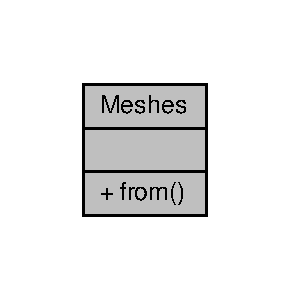
\includegraphics[width=139pt]{structMeshes__coll__graph}
\end{center}
\end{figure}
\subsection*{Public Types}
\begin{DoxyCompactItemize}
\item 
\mbox{\Hypertarget{structMeshes_a17ce7cdf7c4aef0633ce80f5e526b706}\label{structMeshes_a17ce7cdf7c4aef0633ce80f5e526b706}} 
enum {\bfseries value} \{ \newline
{\bfseries Inline\+Line\+With\+Segments}, 
{\bfseries Inline\+Square\+With\+Triangles}, 
{\bfseries Inline\+Square\+With\+Quadrangles}, 
{\bfseries Inline\+Square\+With\+Tetraedres}, 
\newline
{\bfseries Inline\+Square\+With\+Hexaedres}, 
{\bfseries G\+M\+SH}
 \}
\end{DoxyCompactItemize}
\subsection*{Static Public Member Functions}
\begin{DoxyCompactItemize}
\item 
\mbox{\Hypertarget{structMeshes_a41bce2494d7e83bb16a7f79faf1c5d97}\label{structMeshes_a41bce2494d7e83bb16a7f79faf1c5d97}} 
static value {\bfseries from} (const std\+::string \&)
\end{DoxyCompactItemize}


\subsection{Detailed Description}


Definition at line 95 of file Utils/\+Phase\+Field\+Options.\+hpp.



The documentation for this struct was generated from the following file\+:\begin{DoxyCompactItemize}
\item 
Utils/\+Phase\+Field\+Options.\+hpp\end{DoxyCompactItemize}

\hypertarget{structPhaseFieldPrivate_1_1mmap}{}\section{Phase\+Field\+Private\+:\+:mmap$<$ E\+Type $>$ Struct Template Reference}
\label{structPhaseFieldPrivate_1_1mmap}\index{Phase\+Field\+Private\+::mmap$<$ E\+Type $>$@{Phase\+Field\+Private\+::mmap$<$ E\+Type $>$}}


Inheritance diagram for Phase\+Field\+Private\+:\+:mmap$<$ E\+Type $>$\+:\nopagebreak
\begin{figure}[H]
\begin{center}
\leavevmode
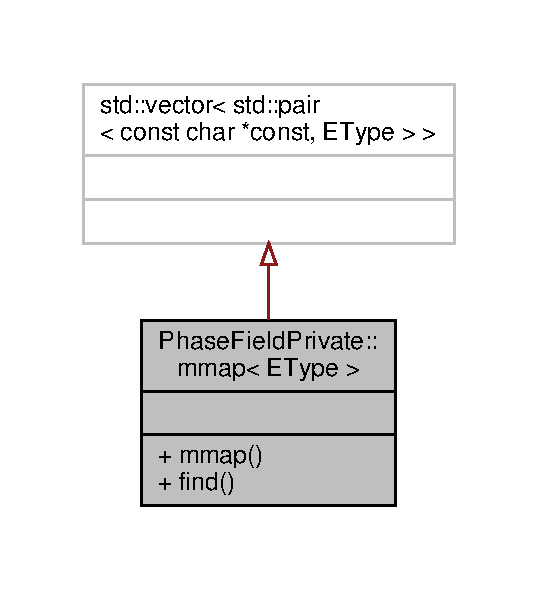
\includegraphics[width=258pt]{structPhaseFieldPrivate_1_1mmap__inherit__graph}
\end{center}
\end{figure}


Collaboration diagram for Phase\+Field\+Private\+:\+:mmap$<$ E\+Type $>$\+:\nopagebreak
\begin{figure}[H]
\begin{center}
\leavevmode
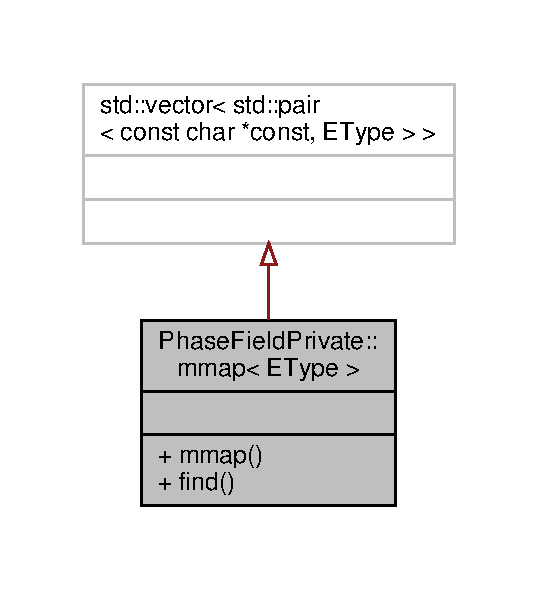
\includegraphics[width=258pt]{structPhaseFieldPrivate_1_1mmap__coll__graph}
\end{center}
\end{figure}
\subsection*{Public Types}
\begin{DoxyCompactItemize}
\item 
\mbox{\Hypertarget{structPhaseFieldPrivate_1_1mmap_a7b38f4b4625451828bc4f491313518de}\label{structPhaseFieldPrivate_1_1mmap_a7b38f4b4625451828bc4f491313518de}} 
using {\bfseries mpair} = std\+::pair$<$ const char $\ast$const, E\+Type $>$
\end{DoxyCompactItemize}
\subsection*{Public Member Functions}
\begin{DoxyCompactItemize}
\item 
\mbox{\Hypertarget{structPhaseFieldPrivate_1_1mmap_aa82b94ef4ad96ca08605b274788428a0}\label{structPhaseFieldPrivate_1_1mmap_aa82b94ef4ad96ca08605b274788428a0}} 
{\bfseries mmap} (const std\+::initializer\+\_\+list$<$ mpair $>$ \&)
\item 
\mbox{\Hypertarget{structPhaseFieldPrivate_1_1mmap_abce88715c469eaf3e4b2856819fbc297}\label{structPhaseFieldPrivate_1_1mmap_abce88715c469eaf3e4b2856819fbc297}} 
E\+Type {\bfseries find} (const char $\ast$const, const std\+::string \&)
\end{DoxyCompactItemize}


\subsection{Detailed Description}
\subsubsection*{template$<$typename E\+Type$>$\newline
struct Phase\+Field\+Private\+::mmap$<$ E\+Type $>$}



Definition at line 21 of file Utils/\+Phase\+Field\+Options.\+hpp.



The documentation for this struct was generated from the following file\+:\begin{DoxyCompactItemize}
\item 
Utils/\+Phase\+Field\+Options.\+hpp\end{DoxyCompactItemize}

\hypertarget{classMobilityCoefficient}{}\section{Mobility\+Coefficient$<$ M\+O\+BI $>$ Class Template Reference}
\label{classMobilityCoefficient}\index{Mobility\+Coefficient$<$ M\+O\+B\+I $>$@{Mobility\+Coefficient$<$ M\+O\+B\+I $>$}}


Inheritance diagram for Mobility\+Coefficient$<$ M\+O\+BI $>$\+:\nopagebreak
\begin{figure}[H]
\begin{center}
\leavevmode
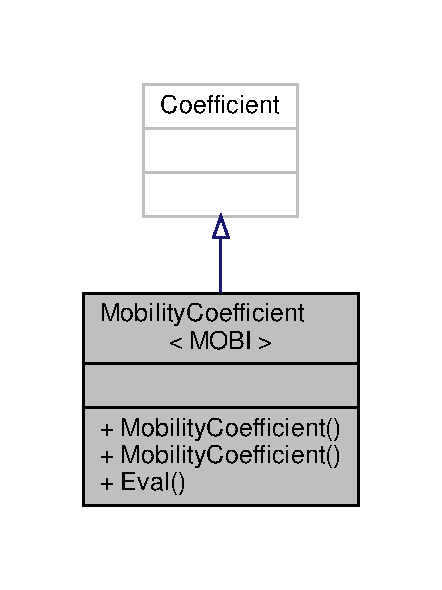
\includegraphics[width=212pt]{classMobilityCoefficient__inherit__graph}
\end{center}
\end{figure}


Collaboration diagram for Mobility\+Coefficient$<$ M\+O\+BI $>$\+:\nopagebreak
\begin{figure}[H]
\begin{center}
\leavevmode
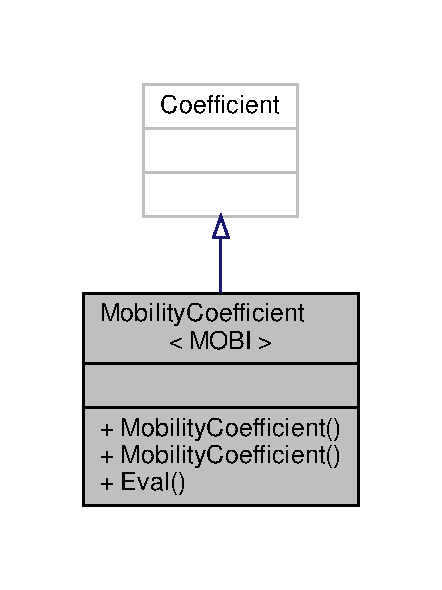
\includegraphics[width=212pt]{classMobilityCoefficient__coll__graph}
\end{center}
\end{figure}
\subsection*{Public Member Functions}
\begin{DoxyCompactItemize}
\item 
\hyperlink{classMobilityCoefficient_a9c91c5b213b6a7c15977fd6d660cb7ed}{Mobility\+Coefficient} (const double \&mob\+\_\+c)
\begin{DoxyCompactList}\small\item\em Construct a new Mobility Coefficient$<$ M\+O\+B\+I$>$\+:\+: Mobility Coefficient object. \end{DoxyCompactList}\item 
\hyperlink{classMobilityCoefficient_a12dab2f5b95a5ab5f6cb01c2d2b5c65c}{Mobility\+Coefficient} (const double \&mob\+\_\+c, mfem\+::\+Grid\+Function mob\+\_\+gf, const int \&order)
\begin{DoxyCompactList}\small\item\em Construct a new Mobility Coefficient$<$ M\+O\+B\+I$>$\+:\+: Mobility Coefficient object. \end{DoxyCompactList}\item 
double \hyperlink{classMobilityCoefficient_a114ed4ca6b17eb4c23c572d6f802c7b2}{Eval} (mfem\+::\+Element\+Transformation \&T, const mfem\+::\+Integration\+Point \&ip)
\begin{DoxyCompactList}\small\item\em Evaluation of the mobility coefficient at integration point. \end{DoxyCompactList}\end{DoxyCompactItemize}


\subsection{Detailed Description}
\subsubsection*{template$<$Mobility M\+O\+BI$>$\newline
class Mobility\+Coefficient$<$ M\+O\+B\+I $>$}



Definition at line 15 of file Mobility\+Coefficient.\+hpp.



\subsection{Constructor \& Destructor Documentation}
\mbox{\Hypertarget{classMobilityCoefficient_a9c91c5b213b6a7c15977fd6d660cb7ed}\label{classMobilityCoefficient_a9c91c5b213b6a7c15977fd6d660cb7ed}} 
\index{Mobility\+Coefficient@{Mobility\+Coefficient}!Mobility\+Coefficient@{Mobility\+Coefficient}}
\index{Mobility\+Coefficient@{Mobility\+Coefficient}!Mobility\+Coefficient@{Mobility\+Coefficient}}
\subsubsection{\texorpdfstring{Mobility\+Coefficient()}{MobilityCoefficient()}\hspace{0.1cm}{\footnotesize\ttfamily [1/2]}}
{\footnotesize\ttfamily template$<$Mobility M\+O\+BI$>$ \\
\hyperlink{classMobilityCoefficient}{Mobility\+Coefficient}$<$ M\+O\+BI $>$\+::\hyperlink{classMobilityCoefficient}{Mobility\+Coefficient} (\begin{DoxyParamCaption}\item[{const double \&}]{mob\+\_\+c }\end{DoxyParamCaption})\hspace{0.3cm}{\ttfamily [explicit]}}



Construct a new Mobility Coefficient$<$ M\+O\+B\+I$>$\+:\+: Mobility Coefficient object. 


\begin{DoxyTemplParams}{Template Parameters}
{\em M\+O\+BI} & \\
\hline
\end{DoxyTemplParams}

\begin{DoxyParams}{Parameters}
{\em mob\+\_\+c} & \\
\hline
\end{DoxyParams}


Definition at line 35 of file Mobility\+Coefficient.\+hpp.


\begin{DoxyCode}
35 : mobility\_(mob\_c) \{\}
\end{DoxyCode}
\mbox{\Hypertarget{classMobilityCoefficient_a12dab2f5b95a5ab5f6cb01c2d2b5c65c}\label{classMobilityCoefficient_a12dab2f5b95a5ab5f6cb01c2d2b5c65c}} 
\index{Mobility\+Coefficient@{Mobility\+Coefficient}!Mobility\+Coefficient@{Mobility\+Coefficient}}
\index{Mobility\+Coefficient@{Mobility\+Coefficient}!Mobility\+Coefficient@{Mobility\+Coefficient}}
\subsubsection{\texorpdfstring{Mobility\+Coefficient()}{MobilityCoefficient()}\hspace{0.1cm}{\footnotesize\ttfamily [2/2]}}
{\footnotesize\ttfamily template$<$Mobility M\+O\+BI$>$ \\
\hyperlink{classMobilityCoefficient}{Mobility\+Coefficient}$<$ M\+O\+BI $>$\+::\hyperlink{classMobilityCoefficient}{Mobility\+Coefficient} (\begin{DoxyParamCaption}\item[{const double \&}]{mob\+\_\+c,  }\item[{mfem\+::\+Grid\+Function}]{mob\+\_\+gf,  }\item[{const int \&}]{order }\end{DoxyParamCaption})}



Construct a new Mobility Coefficient$<$ M\+O\+B\+I$>$\+:\+: Mobility Coefficient object. 


\begin{DoxyTemplParams}{Template Parameters}
{\em M\+O\+BI} & \\
\hline
\end{DoxyTemplParams}

\begin{DoxyParams}{Parameters}
{\em mob\+\_\+c} & \\
\hline
{\em mob\+\_\+gf} & \\
\hline
{\em order} & \\
\hline
\end{DoxyParams}


Definition at line 46 of file Mobility\+Coefficient.\+hpp.


\begin{DoxyCode}
48     : mobility\_(mob\_c), gf(mob\_gf), degenerate\_order\_(order) \{\}
\end{DoxyCode}


\subsection{Member Function Documentation}
\mbox{\Hypertarget{classMobilityCoefficient_a114ed4ca6b17eb4c23c572d6f802c7b2}\label{classMobilityCoefficient_a114ed4ca6b17eb4c23c572d6f802c7b2}} 
\index{Mobility\+Coefficient@{Mobility\+Coefficient}!Eval@{Eval}}
\index{Eval@{Eval}!Mobility\+Coefficient@{Mobility\+Coefficient}}
\subsubsection{\texorpdfstring{Eval()}{Eval()}}
{\footnotesize\ttfamily template$<$Mobility M\+O\+BI$>$ \\
double \hyperlink{classMobilityCoefficient}{Mobility\+Coefficient}$<$ M\+O\+BI $>$\+::Eval (\begin{DoxyParamCaption}\item[{mfem\+::\+Element\+Transformation \&}]{T,  }\item[{const mfem\+::\+Integration\+Point \&}]{ip }\end{DoxyParamCaption})}



Evaluation of the mobility coefficient at integration point. 


\begin{DoxyTemplParams}{Template Parameters}
{\em M\+O\+BI} & \\
\hline
\end{DoxyTemplParams}

\begin{DoxyParams}{Parameters}
{\em T} & \\
\hline
{\em ip} & \\
\hline
\end{DoxyParams}
\begin{DoxyReturn}{Returns}
double 
\end{DoxyReturn}


Definition at line 59 of file Mobility\+Coefficient.\+hpp.


\begin{DoxyCode}
60                                                                        \{
61   \textcolor{keywordflow}{switch} (MOBI) \{
62     \textcolor{keywordflow}{case} Mobility::Constant:
63       \textcolor{keywordflow}{return} this->mobility\_;
64     \textcolor{keywordflow}{case} Mobility::Degenerated:
65       \textcolor{keyword}{const} \textcolor{keyword}{auto} xx = gf.GetValue(T.ElementNo, ip);
66       \textcolor{keyword}{const} \textcolor{keyword}{auto} a\_xx = std::max(std::min(xx, 1.), 0.);
67       \textcolor{keyword}{const} \textcolor{keyword}{auto} degenerated\_mob\_func = this->mobility\_ *
68                                         std::pow(1. - a\_xx, this->degenerate\_order\_) *
69                                         std::pow(a\_xx, this->degenerate\_order\_);
70       \textcolor{keywordflow}{return} degenerated\_mob\_func;
71     \textcolor{keywordflow}{default}:
72       \textcolor{keywordflow}{throw} std::runtime\_error(
73           \textcolor{stringliteral}{"MobilityCoefficient::Eval: only constant and degenerated mobilities  are available"});
74       \textcolor{keywordflow}{break};
75   \}
76 \}
\end{DoxyCode}


The documentation for this class was generated from the following file\+:\begin{DoxyCompactItemize}
\item 
Mobility\+Coefficient.\+hpp\end{DoxyCompactItemize}

\hypertarget{classMobilityFunctions}{}\section{Mobility\+Functions$<$ M\+O\+BI $>$ Class Template Reference}
\label{classMobilityFunctions}\index{Mobility\+Functions$<$ M\+O\+B\+I $>$@{Mobility\+Functions$<$ M\+O\+B\+I $>$}}


Collaboration diagram for Mobility\+Functions$<$ M\+O\+BI $>$\+:\nopagebreak
\begin{figure}[H]
\begin{center}
\leavevmode
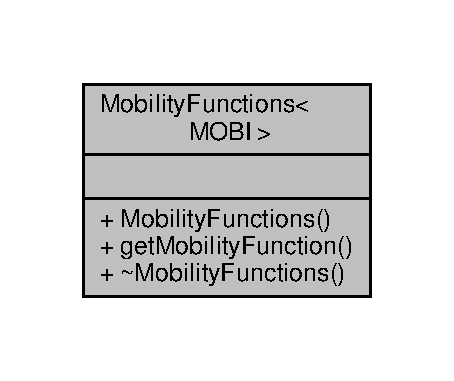
\includegraphics[width=218pt]{classMobilityFunctions__coll__graph}
\end{center}
\end{figure}
\subsection*{Public Member Functions}
\begin{DoxyCompactItemize}
\item 
\mbox{\Hypertarget{classMobilityFunctions_add3cbc5101d579b77a2c2963e8008101}\label{classMobilityFunctions_add3cbc5101d579b77a2c2963e8008101}} 
\hyperlink{classMobilityFunctions_add3cbc5101d579b77a2c2963e8008101}{Mobility\+Functions} ()
\begin{DoxyCompactList}\small\item\em Construct a new potential function\+:\+: potential function object. \end{DoxyCompactList}\item 
{\footnotesize template$<$class... Args$>$ }\\std\+::function$<$ double(const double \&)$>$ \hyperlink{classMobilityFunctions_a25741d28fd09272b2647f5af944aa748}{get\+Mobility\+Function} (Args... args)
\begin{DoxyCompactList}\small\item\em return the function associated with the potential\+\_\+name and its O\+R\+D\+ER of derivative \end{DoxyCompactList}\item 
\mbox{\Hypertarget{classMobilityFunctions_aef50ad1966cd9afc7b61ab5eb25df771}\label{classMobilityFunctions_aef50ad1966cd9afc7b61ab5eb25df771}} 
\hyperlink{classMobilityFunctions_aef50ad1966cd9afc7b61ab5eb25df771}{$\sim$\+Mobility\+Functions} ()
\begin{DoxyCompactList}\small\item\em Destroy the potential function \+:\+: potential function object. \end{DoxyCompactList}\end{DoxyCompactItemize}


\subsection{Detailed Description}
\subsubsection*{template$<$Mobility M\+O\+BI$>$\newline
class Mobility\+Functions$<$ M\+O\+B\+I $>$}



Definition at line 21 of file Phase\+Field\+Mobilities.\+hpp.



\subsection{Member Function Documentation}
\mbox{\Hypertarget{classMobilityFunctions_a25741d28fd09272b2647f5af944aa748}\label{classMobilityFunctions_a25741d28fd09272b2647f5af944aa748}} 
\index{Mobility\+Functions@{Mobility\+Functions}!get\+Mobility\+Function@{get\+Mobility\+Function}}
\index{get\+Mobility\+Function@{get\+Mobility\+Function}!Mobility\+Functions@{Mobility\+Functions}}
\subsubsection{\texorpdfstring{get\+Mobility\+Function()}{getMobilityFunction()}}
{\footnotesize\ttfamily template$<$Mobility M\+O\+BI$>$ \\
template$<$class... Args$>$ \\
std\+::function$<$ double(const double \&)$>$ \hyperlink{classMobilityFunctions}{Mobility\+Functions}$<$ M\+O\+BI $>$\+::get\+Mobility\+Function (\begin{DoxyParamCaption}\item[{Args...}]{args }\end{DoxyParamCaption})}



return the function associated with the potential\+\_\+name and its O\+R\+D\+ER of derivative 


\begin{DoxyParams}{Parameters}
{\em potential\+\_\+name} & \\
\hline
\end{DoxyParams}
\begin{DoxyReturn}{Returns}
const double 
\end{DoxyReturn}


Definition at line 99 of file Phase\+Field\+Mobilities.\+hpp.


\begin{DoxyCode}
99                                                                                             \{
100   \textcolor{keywordflow}{switch} (MOBI) \{
101     \textcolor{keywordflow}{case} Mobility::Constant:
102       \textcolor{keywordflow}{return} this->getConstant(args...);
103     \textcolor{keywordflow}{case} Mobility::Degenerated:
104       \textcolor{keywordflow}{return} this->getDegenerated(args...);
105     \textcolor{keywordflow}{default}:
106       \textcolor{keywordflow}{throw} std::runtime\_error(
107           \textcolor{stringliteral}{"MobilityFunctions::getMobilityFunctions: only constant and degenerated mobilities  are "}
108           \textcolor{stringliteral}{"available"});
109       \textcolor{keywordflow}{break};
110   \}
111 \}
\end{DoxyCode}


The documentation for this class was generated from the following file\+:\begin{DoxyCompactItemize}
\item 
Phase\+Field\+Mobilities.\+hpp\end{DoxyCompactItemize}

\hypertarget{structmultidimension__function}{}\section{multidimension\+\_\+function$<$ D\+IM $>$ Struct Template Reference}
\label{structmultidimension__function}\index{multidimension\+\_\+function$<$ D\+I\+M $>$@{multidimension\+\_\+function$<$ D\+I\+M $>$}}


Collaboration diagram for multidimension\+\_\+function$<$ D\+IM $>$\+:\nopagebreak
\begin{figure}[H]
\begin{center}
\leavevmode
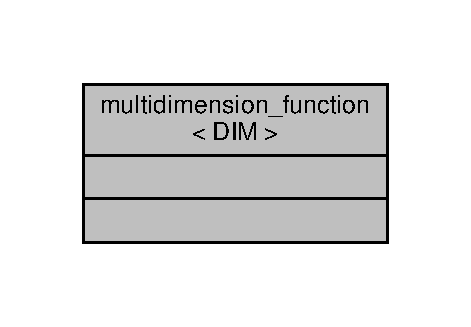
\includegraphics[width=226pt]{structmultidimension__function__coll__graph}
\end{center}
\end{figure}


\subsection{Detailed Description}
\subsubsection*{template$<$int D\+IM$>$\newline
struct multidimension\+\_\+function$<$ D\+I\+M $>$}



Definition at line 21 of file Utils/\+Analytical\+Functions.\+hpp.



The documentation for this struct was generated from the following file\+:\begin{DoxyCompactItemize}
\item 
Utils/\+Analytical\+Functions.\+hpp\end{DoxyCompactItemize}

\hypertarget{structmultidimension__function_3_011_01_4}{}\section{multidimension\+\_\+function$<$ 1 $>$ Struct Template Reference}
\label{structmultidimension__function_3_011_01_4}\index{multidimension\+\_\+function$<$ 1 $>$@{multidimension\+\_\+function$<$ 1 $>$}}


Collaboration diagram for multidimension\+\_\+function$<$ 1 $>$\+:\nopagebreak
\begin{figure}[H]
\begin{center}
\leavevmode
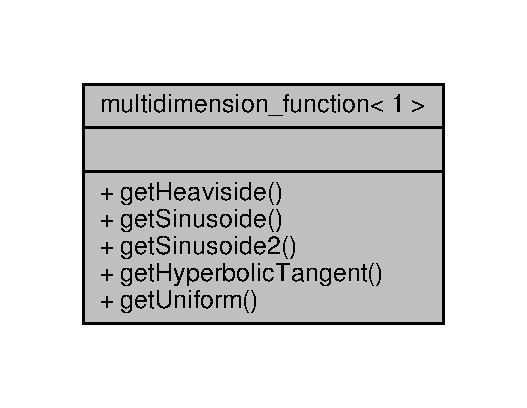
\includegraphics[width=253pt]{structmultidimension__function_3_011_01_4__coll__graph}
\end{center}
\end{figure}
\subsection*{Public Member Functions}
\begin{DoxyCompactItemize}
\item 
\mbox{\Hypertarget{structmultidimension__function_3_011_01_4_ad320d1f228f9feb1370882f576629e86}\label{structmultidimension__function_3_011_01_4_ad320d1f228f9feb1370882f576629e86}} 
{\footnotesize template$<$typename... Args$>$ }\\std\+::function$<$ double(const mfem\+::\+Vector \&, double)$>$ {\bfseries get\+Heaviside} (Args... args)
\item 
\mbox{\Hypertarget{structmultidimension__function_3_011_01_4_a8592270b8cb9c2036bfe9ccab1471c21}\label{structmultidimension__function_3_011_01_4_a8592270b8cb9c2036bfe9ccab1471c21}} 
{\footnotesize template$<$typename... Args$>$ }\\std\+::function$<$ double(const mfem\+::\+Vector \&, double)$>$ {\bfseries get\+Sinusoide} (Args... args)
\item 
\mbox{\Hypertarget{structmultidimension__function_3_011_01_4_a084dd30c744c719e8dd9af6b13f53c0d}\label{structmultidimension__function_3_011_01_4_a084dd30c744c719e8dd9af6b13f53c0d}} 
{\footnotesize template$<$typename... Args$>$ }\\std\+::function$<$ double(const mfem\+::\+Vector \&, double)$>$ {\bfseries get\+Sinusoide2} (Args... args)
\item 
\mbox{\Hypertarget{structmultidimension__function_3_011_01_4_acd5d0fee883c406f239e20ce3e8a4c87}\label{structmultidimension__function_3_011_01_4_acd5d0fee883c406f239e20ce3e8a4c87}} 
{\footnotesize template$<$typename... Args$>$ }\\std\+::function$<$ double(const mfem\+::\+Vector \&, double)$>$ {\bfseries get\+Hyperbolic\+Tangent} (Args... args)
\item 
\mbox{\Hypertarget{structmultidimension__function_3_011_01_4_a75f7260a054bddf709fb78989cecda3e}\label{structmultidimension__function_3_011_01_4_a75f7260a054bddf709fb78989cecda3e}} 
{\footnotesize template$<$typename... Args$>$ }\\std\+::function$<$ double(const mfem\+::\+Vector \&, double)$>$ {\bfseries get\+Uniform} (Args... args)
\end{DoxyCompactItemize}


\subsection{Detailed Description}
\subsubsection*{template$<$$>$\newline
struct multidimension\+\_\+function$<$ 1 $>$}



Definition at line 68 of file Utils/\+Analytical\+Functions.\+hpp.



The documentation for this struct was generated from the following file\+:\begin{DoxyCompactItemize}
\item 
Utils/\+Analytical\+Functions.\+hpp\end{DoxyCompactItemize}

\hypertarget{structmultidimension__function_3_012_01_4}{}\section{multidimension\+\_\+function$<$ 2 $>$ Struct Template Reference}
\label{structmultidimension__function_3_012_01_4}\index{multidimension\+\_\+function$<$ 2 $>$@{multidimension\+\_\+function$<$ 2 $>$}}


Collaboration diagram for multidimension\+\_\+function$<$ 2 $>$\+:\nopagebreak
\begin{figure}[H]
\begin{center}
\leavevmode
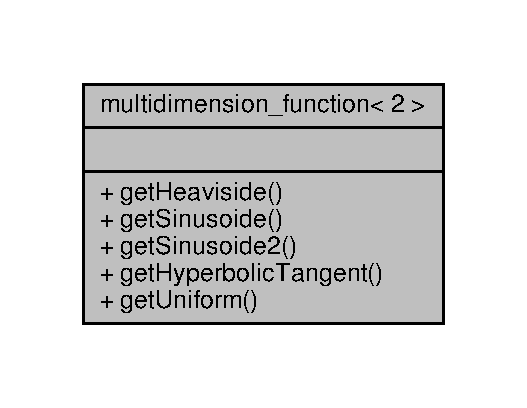
\includegraphics[width=253pt]{structmultidimension__function_3_012_01_4__coll__graph}
\end{center}
\end{figure}
\subsection*{Public Member Functions}
\begin{DoxyCompactItemize}
\item 
\mbox{\Hypertarget{structmultidimension__function_3_012_01_4_a57644b2f98088bc9ca6ef60b0cdda308}\label{structmultidimension__function_3_012_01_4_a57644b2f98088bc9ca6ef60b0cdda308}} 
{\footnotesize template$<$typename... Args$>$ }\\std\+::function$<$ double(const mfem\+::\+Vector \&, double)$>$ {\bfseries get\+Heaviside} (Args... args)
\item 
\mbox{\Hypertarget{structmultidimension__function_3_012_01_4_a84167984fca9d03ed09c528fee67a365}\label{structmultidimension__function_3_012_01_4_a84167984fca9d03ed09c528fee67a365}} 
{\footnotesize template$<$typename... Args$>$ }\\std\+::function$<$ double(const mfem\+::\+Vector \&, double)$>$ {\bfseries get\+Sinusoide} (Args... args)
\item 
\mbox{\Hypertarget{structmultidimension__function_3_012_01_4_a5c0f91967557dc8578bce376514db43c}\label{structmultidimension__function_3_012_01_4_a5c0f91967557dc8578bce376514db43c}} 
{\footnotesize template$<$typename... Args$>$ }\\std\+::function$<$ double(const mfem\+::\+Vector \&, double)$>$ {\bfseries get\+Sinusoide2} (Args... args)
\item 
\mbox{\Hypertarget{structmultidimension__function_3_012_01_4_a08d7787f61939dbc258ae83aaf9e0590}\label{structmultidimension__function_3_012_01_4_a08d7787f61939dbc258ae83aaf9e0590}} 
{\footnotesize template$<$typename... Args$>$ }\\std\+::function$<$ double(const mfem\+::\+Vector \&, double)$>$ {\bfseries get\+Hyperbolic\+Tangent} (Args... args)
\item 
\mbox{\Hypertarget{structmultidimension__function_3_012_01_4_a54db4b923a00f045f16094b3e2531d83}\label{structmultidimension__function_3_012_01_4_a54db4b923a00f045f16094b3e2531d83}} 
{\footnotesize template$<$typename... Args$>$ }\\std\+::function$<$ double(const mfem\+::\+Vector \&, double)$>$ {\bfseries get\+Uniform} (Args... args)
\end{DoxyCompactItemize}


\subsection{Detailed Description}
\subsubsection*{template$<$$>$\newline
struct multidimension\+\_\+function$<$ 2 $>$}



Definition at line 127 of file Utils/\+Analytical\+Functions.\+hpp.



The documentation for this struct was generated from the following file\+:\begin{DoxyCompactItemize}
\item 
Utils/\+Analytical\+Functions.\+hpp\end{DoxyCompactItemize}

\hypertarget{structmultidimension__function_3_013_01_4}{}\section{multidimension\+\_\+function$<$ 3 $>$ Struct Template Reference}
\label{structmultidimension__function_3_013_01_4}\index{multidimension\+\_\+function$<$ 3 $>$@{multidimension\+\_\+function$<$ 3 $>$}}


Collaboration diagram for multidimension\+\_\+function$<$ 3 $>$\+:\nopagebreak
\begin{figure}[H]
\begin{center}
\leavevmode
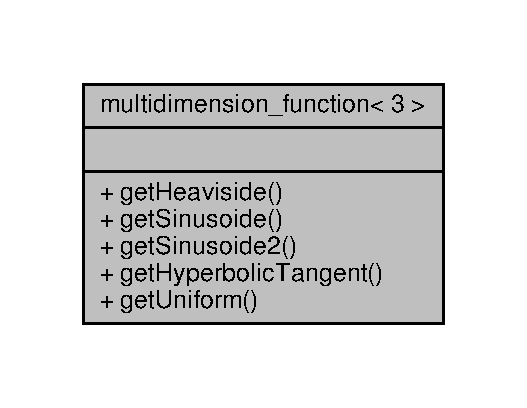
\includegraphics[width=253pt]{structmultidimension__function_3_013_01_4__coll__graph}
\end{center}
\end{figure}
\subsection*{Public Member Functions}
\begin{DoxyCompactItemize}
\item 
\mbox{\Hypertarget{structmultidimension__function_3_013_01_4_af11a5af155caff37e8ecea23420cd159}\label{structmultidimension__function_3_013_01_4_af11a5af155caff37e8ecea23420cd159}} 
{\footnotesize template$<$typename... Args$>$ }\\std\+::function$<$ double(const mfem\+::\+Vector \&, double)$>$ {\bfseries get\+Heaviside} (Args... args)
\item 
\mbox{\Hypertarget{structmultidimension__function_3_013_01_4_acfed713a1cccbfa2dfcaec0e167c62e3}\label{structmultidimension__function_3_013_01_4_acfed713a1cccbfa2dfcaec0e167c62e3}} 
{\footnotesize template$<$typename... Args$>$ }\\std\+::function$<$ double(const mfem\+::\+Vector \&, double)$>$ {\bfseries get\+Sinusoide} (Args... args)
\item 
\mbox{\Hypertarget{structmultidimension__function_3_013_01_4_a9d5fb5174a35dc8c491481756c927f7a}\label{structmultidimension__function_3_013_01_4_a9d5fb5174a35dc8c491481756c927f7a}} 
{\footnotesize template$<$typename... Args$>$ }\\std\+::function$<$ double(const mfem\+::\+Vector \&, double)$>$ {\bfseries get\+Sinusoide2} (Args... args)
\item 
\mbox{\Hypertarget{structmultidimension__function_3_013_01_4_ae32120bf1dc07b6ca836d942126162f2}\label{structmultidimension__function_3_013_01_4_ae32120bf1dc07b6ca836d942126162f2}} 
{\footnotesize template$<$typename... Args$>$ }\\std\+::function$<$ double(const mfem\+::\+Vector \&, double)$>$ {\bfseries get\+Hyperbolic\+Tangent} (Args... args)
\item 
\mbox{\Hypertarget{structmultidimension__function_3_013_01_4_a9c5a0ce462becae15cea32131b77aaa7}\label{structmultidimension__function_3_013_01_4_a9c5a0ce462becae15cea32131b77aaa7}} 
{\footnotesize template$<$typename... Args$>$ }\\std\+::function$<$ double(const mfem\+::\+Vector \&, double)$>$ {\bfseries get\+Uniform} (Args... args)
\end{DoxyCompactItemize}


\subsection{Detailed Description}
\subsubsection*{template$<$$>$\newline
struct multidimension\+\_\+function$<$ 3 $>$}



Definition at line 215 of file Utils/\+Analytical\+Functions.\+hpp.



The documentation for this struct was generated from the following file\+:\begin{DoxyCompactItemize}
\item 
Utils/\+Analytical\+Functions.\+hpp\end{DoxyCompactItemize}

\hypertarget{classNonlinearCoefficient}{}\section{Nonlinear\+Coefficient Class Reference}
\label{classNonlinearCoefficient}\index{Nonlinear\+Coefficient@{Nonlinear\+Coefficient}}


{\ttfamily \#include $<$/home/ci230846/home-\/local/\+My\+Git\+Projects/\+C\+O\+M\+P\+O\+N\+E\+N\+T/\+P\+F-\/\+M\+F\+E\+M/\+Integrators/\+Diffusion\+N\+L\+F\+Integrator.\+hpp$>$}



Inheritance diagram for Nonlinear\+Coefficient\+:\nopagebreak
\begin{figure}[H]
\begin{center}
\leavevmode
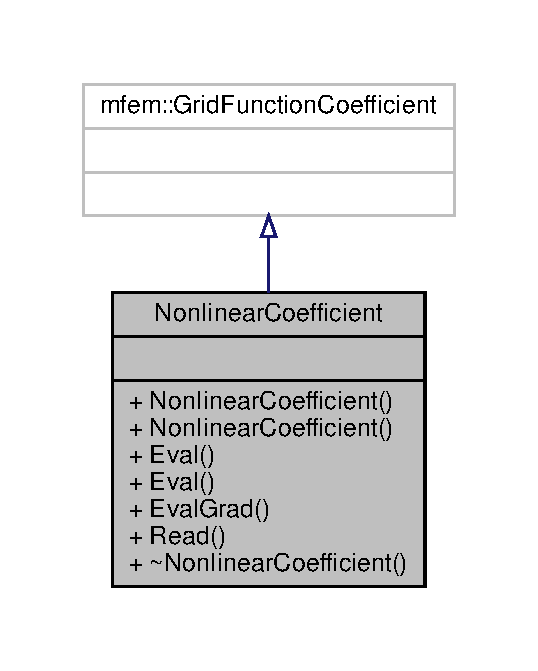
\includegraphics[width=258pt]{classNonlinearCoefficient__inherit__graph}
\end{center}
\end{figure}


Collaboration diagram for Nonlinear\+Coefficient\+:\nopagebreak
\begin{figure}[H]
\begin{center}
\leavevmode
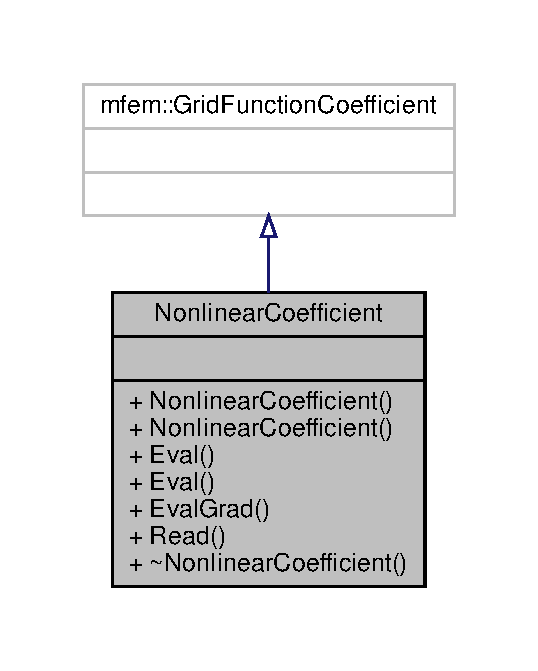
\includegraphics[width=258pt]{classNonlinearCoefficient__coll__graph}
\end{center}
\end{figure}
\subsection*{Public Member Functions}
\begin{DoxyCompactItemize}
\item 
\mbox{\Hypertarget{classNonlinearCoefficient_af9d31aa89191469de92d80e48637c64f}\label{classNonlinearCoefficient_af9d31aa89191469de92d80e48637c64f}} 
{\bfseries Nonlinear\+Coefficient} (double rho\+\_\+, double bt\+\_\+, double p0)
\item 
\mbox{\Hypertarget{classNonlinearCoefficient_a41db0c64a3dfcf1dbbea6630bd2ee193}\label{classNonlinearCoefficient_a41db0c64a3dfcf1dbbea6630bd2ee193}} 
{\bfseries Nonlinear\+Coefficient} (mfem\+::\+Grid\+Function $\ast$u\+\_\+, double rho\+\_\+, double bt\+\_\+, double p0)
\item 
\mbox{\Hypertarget{classNonlinearCoefficient_aa979c936709c19e3089aa9f60354225b}\label{classNonlinearCoefficient_aa979c936709c19e3089aa9f60354225b}} 
virtual double {\bfseries Eval} (mfem\+::\+Element\+Transformation \&T, const mfem\+::\+Integration\+Point \&ip)
\item 
\mbox{\Hypertarget{classNonlinearCoefficient_a1ea6e8519bc3eac3c0976f077596b71b}\label{classNonlinearCoefficient_a1ea6e8519bc3eac3c0976f077596b71b}} 
virtual double {\bfseries Eval} (mfem\+::\+Element\+Transformation \&T, const mfem\+::\+Integration\+Point \&ip, const double \&u)
\item 
\mbox{\Hypertarget{classNonlinearCoefficient_a55197365c8257b2cd5a75b87bbb8a36e}\label{classNonlinearCoefficient_a55197365c8257b2cd5a75b87bbb8a36e}} 
virtual double {\bfseries Eval\+Grad} (mfem\+::\+Element\+Transformation \&T, const mfem\+::\+Integration\+Point \&ip, const double \&u)
\item 
\mbox{\Hypertarget{classNonlinearCoefficient_abc449e82f5d99e5dbd9fcc128880bda0}\label{classNonlinearCoefficient_abc449e82f5d99e5dbd9fcc128880bda0}} 
virtual void {\bfseries Read} (std\+::istream \&in)
\end{DoxyCompactItemize}


\subsection{Detailed Description}
Function representing a nonlinear coefficient (density) for the given state (pressure). Used in \hyperlink{classDiffusionNLFIntegrator_ac7b70b5cee3c880d52b03a87706ae8e3}{Diffusion\+N\+L\+F\+Integrator\+::\+Assemble\+Element\+Grad}. 

Definition at line 13 of file Diffusion\+N\+L\+F\+Integrator.\+hpp.



The documentation for this class was generated from the following file\+:\begin{DoxyCompactItemize}
\item 
Diffusion\+N\+L\+F\+Integrator.\+hpp\end{DoxyCompactItemize}

\hypertarget{classParameter}{}\section{Parameter Class Reference}
\label{classParameter}\index{Parameter@{Parameter}}


Collaboration diagram for Parameter\+:\nopagebreak
\begin{figure}[H]
\begin{center}
\leavevmode
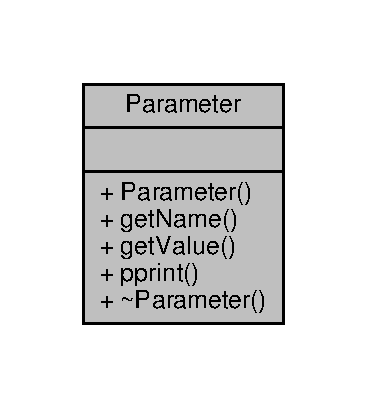
\includegraphics[width=176pt]{classParameter__coll__graph}
\end{center}
\end{figure}
\subsection*{Public Member Functions}
\begin{DoxyCompactItemize}
\item 
\mbox{\Hypertarget{classParameter_ad97fb10933adaa11fe8d4a3222ec72c2}\label{classParameter_ad97fb10933adaa11fe8d4a3222ec72c2}} 
{\bfseries Parameter} (std\+::string name, var value)
\item 
std\+::string \hyperlink{classParameter_a6687b858b004ed892c764f86b9a1c965}{get\+Name} () const
\item 
var \hyperlink{classParameter_acb6003c8455f06d2191af29524142b16}{get\+Value} () const
\item 
\mbox{\Hypertarget{classParameter_a49b4f1c57d65b634d7f5fd14bddd587f}\label{classParameter_a49b4f1c57d65b634d7f5fd14bddd587f}} 
void {\bfseries pprint} ()
\end{DoxyCompactItemize}


\subsection{Detailed Description}


Definition at line 18 of file Parameter.\+hpp.



\subsection{Member Function Documentation}
\mbox{\Hypertarget{classParameter_a6687b858b004ed892c764f86b9a1c965}\label{classParameter_a6687b858b004ed892c764f86b9a1c965}} 
\index{Parameter@{Parameter}!get\+Name@{get\+Name}}
\index{get\+Name@{get\+Name}!Parameter@{Parameter}}
\subsubsection{\texorpdfstring{get\+Name()}{getName()}}
{\footnotesize\ttfamily std\+::string Parameter\+::get\+Name (\begin{DoxyParamCaption}{ }\end{DoxyParamCaption}) const\hspace{0.3cm}{\ttfamily [inline]}}

Method used to get the name of the parameter return name of the parameter of type string 

Definition at line 31 of file Parameter.\+hpp.


\begin{DoxyCode}
31 \{ \textcolor{keywordflow}{return} name; \}  \textcolor{comment}{// end of getName}
\end{DoxyCode}
\mbox{\Hypertarget{classParameter_acb6003c8455f06d2191af29524142b16}\label{classParameter_acb6003c8455f06d2191af29524142b16}} 
\index{Parameter@{Parameter}!get\+Value@{get\+Value}}
\index{get\+Value@{get\+Value}!Parameter@{Parameter}}
\subsubsection{\texorpdfstring{get\+Value()}{getValue()}}
{\footnotesize\ttfamily var Parameter\+::get\+Value (\begin{DoxyParamCaption}{ }\end{DoxyParamCaption}) const\hspace{0.3cm}{\ttfamily [inline]}}

Method used to get the value of the parameter return value of the parameter of any type (see variant) 

Definition at line 36 of file Parameter.\+hpp.


\begin{DoxyCode}
36 \{ \textcolor{keywordflow}{return} value; \}  \textcolor{comment}{// end of getValue}
\end{DoxyCode}


The documentation for this class was generated from the following file\+:\begin{DoxyCompactItemize}
\item 
Parameter.\+hpp\end{DoxyCompactItemize}

\hypertarget{classParameters}{}\section{Parameters Class Reference}
\label{classParameters}\index{Parameters@{Parameters}}


Class used to manage a list of \hyperlink{classParameter}{Parameter}.  




{\ttfamily \#include $<$/home/ci230846/home-\/local/\+My\+Git\+Projects/\+C\+O\+M\+P\+O\+N\+E\+N\+T/\+P\+F-\/\+M\+F\+E\+M/\+Parameters/\+Parameters.\+hpp$>$}



Collaboration diagram for Parameters\+:\nopagebreak
\begin{figure}[H]
\begin{center}
\leavevmode
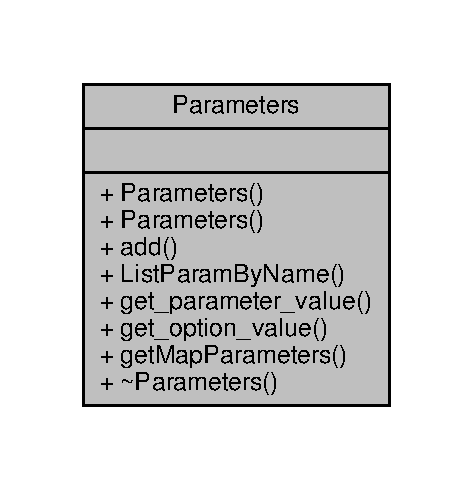
\includegraphics[width=227pt]{classParameters__coll__graph}
\end{center}
\end{figure}
\subsection*{Public Member Functions}
\begin{DoxyCompactItemize}
\item 
\mbox{\Hypertarget{classParameters_af4d94ee360ac0157d9065f78797fe9a1}\label{classParameters_af4d94ee360ac0157d9065f78797fe9a1}} 
\hyperlink{classParameters_af4d94ee360ac0157d9065f78797fe9a1}{Parameters} ()
\begin{DoxyCompactList}\small\item\em Construct a new \hyperlink{classParameters}{Parameters}\+:\+: \hyperlink{classParameters}{Parameters} object. \end{DoxyCompactList}\item 
{\footnotesize template$<$class... Args$>$ }\\\hyperlink{classParameters_ad6dd615ae7b15ad277796f0ea5d15442}{Parameters} (const Args \&... args)
\begin{DoxyCompactList}\small\item\em Construct a new \hyperlink{classParameters}{Parameters}\+:\+: \hyperlink{classParameters}{Parameters} object. \end{DoxyCompactList}\item 
void \hyperlink{classParameters_a0e846d18b12895afa22311f4b597ff90}{add} (const \hyperlink{classParameter}{Parameter} \&param)
\begin{DoxyCompactList}\small\item\em add a new parameters \end{DoxyCompactList}\item 
\mbox{\Hypertarget{classParameters_a54c52e1c269e995779f16f33f4c68db0}\label{classParameters_a54c52e1c269e995779f16f33f4c68db0}} 
void {\bfseries List\+Param\+By\+Name} ()
\item 
double \hyperlink{classParameters_ab1bac6bf07b9698c850542b68e143ef3}{get\+\_\+parameter\+\_\+value} (const std\+::string \&name) const
\begin{DoxyCompactList}\small\item\em get double value of a parameter by name \end{DoxyCompactList}\item 
bool \hyperlink{classParameters_a33402b196d17c9f3816f9c889b87c540}{get\+\_\+option\+\_\+value} (const std\+::string \&name) const
\begin{DoxyCompactList}\small\item\em get boolean option of a parameter by name \end{DoxyCompactList}\item 
std\+::map$<$ std\+::string, double $>$ \hyperlink{classParameters_a3951bee7d4347d18d528cd0f5c3a2e67}{get\+Map\+Parameters} () const
\begin{DoxyCompactList}\small\item\em transform list of parameters into a map$<$string,double$>$ \end{DoxyCompactList}\item 
\mbox{\Hypertarget{classParameters_a640a1a349975a8cb023696f25e563a5c}\label{classParameters_a640a1a349975a8cb023696f25e563a5c}} 
\hyperlink{classParameters_a640a1a349975a8cb023696f25e563a5c}{$\sim$\+Parameters} ()
\begin{DoxyCompactList}\small\item\em Destroy the \hyperlink{classParameters}{Parameters}\+:\+: \hyperlink{classParameters}{Parameters} object. \end{DoxyCompactList}\end{DoxyCompactItemize}


\subsection{Detailed Description}
Class used to manage a list of \hyperlink{classParameter}{Parameter}. 

Definition at line 23 of file Parameters.\+hpp.



\subsection{Constructor \& Destructor Documentation}
\mbox{\Hypertarget{classParameters_ad6dd615ae7b15ad277796f0ea5d15442}\label{classParameters_ad6dd615ae7b15ad277796f0ea5d15442}} 
\index{Parameters@{Parameters}!Parameters@{Parameters}}
\index{Parameters@{Parameters}!Parameters@{Parameters}}
\subsubsection{\texorpdfstring{Parameters()}{Parameters()}}
{\footnotesize\ttfamily template$<$class... Args$>$ \\
Parameters\+::\+Parameters (\begin{DoxyParamCaption}\item[{const Args \&...}]{args }\end{DoxyParamCaption})\hspace{0.3cm}{\ttfamily [explicit]}}



Construct a new \hyperlink{classParameters}{Parameters}\+:\+: \hyperlink{classParameters}{Parameters} object. 


\begin{DoxyTemplParams}{Template Parameters}
{\em Args} & \\
\hline
\end{DoxyTemplParams}

\begin{DoxyParams}{Parameters}
{\em args} & \\
\hline
\end{DoxyParams}


Definition at line 53 of file Parameters.\+hpp.


\begin{DoxyCode}
53                                           \{
54   this->vect\_params\_ = std::vector<Parameter>\{args...\};
55 \}
\end{DoxyCode}


\subsection{Member Function Documentation}
\mbox{\Hypertarget{classParameters_a0e846d18b12895afa22311f4b597ff90}\label{classParameters_a0e846d18b12895afa22311f4b597ff90}} 
\index{Parameters@{Parameters}!add@{add}}
\index{add@{add}!Parameters@{Parameters}}
\subsubsection{\texorpdfstring{add()}{add()}}
{\footnotesize\ttfamily void Parameters\+::add (\begin{DoxyParamCaption}\item[{const \hyperlink{classParameter}{Parameter} \&}]{param }\end{DoxyParamCaption})}



add a new parameters 


\begin{DoxyParams}{Parameters}
{\em param} & parameter to add \\
\hline
\end{DoxyParams}


Definition at line 62 of file Parameters.\+hpp.


\begin{DoxyCode}
62 \{ this->vect\_params\_.emplace\_back(param); \}
\end{DoxyCode}
\mbox{\Hypertarget{classParameters_a33402b196d17c9f3816f9c889b87c540}\label{classParameters_a33402b196d17c9f3816f9c889b87c540}} 
\index{Parameters@{Parameters}!get\+\_\+option\+\_\+value@{get\+\_\+option\+\_\+value}}
\index{get\+\_\+option\+\_\+value@{get\+\_\+option\+\_\+value}!Parameters@{Parameters}}
\subsubsection{\texorpdfstring{get\+\_\+option\+\_\+value()}{get\_option\_value()}}
{\footnotesize\ttfamily bool Parameters\+::get\+\_\+option\+\_\+value (\begin{DoxyParamCaption}\item[{const std\+::string \&}]{name }\end{DoxyParamCaption}) const}



get boolean option of a parameter by name 


\begin{DoxyParams}{Parameters}
{\em name} & \\
\hline
\end{DoxyParams}
\begin{DoxyReturn}{Returns}
true 

false 
\end{DoxyReturn}


Definition at line 94 of file Parameters.\+hpp.



Referenced by Time\+Discretization$<$ T, D\+C, D\+I\+M $>$\+::\+Time\+Discretization().


\begin{DoxyCode}
94                                                              \{
95   \textcolor{keywordtype}{bool} active\_option = \textcolor{keyword}{false};
96 
97   \textcolor{keywordflow}{for} (\textcolor{keyword}{const} \textcolor{keyword}{auto}& p : this->vect\_params\_) \{
98     \textcolor{keyword}{auto} pn = p.getName();
99     \textcolor{keywordflow}{if} (pn == name) \{
100       active\_option = std::get<bool>(p.getValue());
101     \}
102   \}
103 
104   \textcolor{keywordflow}{return} active\_option;
105 \}
\end{DoxyCode}
\mbox{\Hypertarget{classParameters_ab1bac6bf07b9698c850542b68e143ef3}\label{classParameters_ab1bac6bf07b9698c850542b68e143ef3}} 
\index{Parameters@{Parameters}!get\+\_\+parameter\+\_\+value@{get\+\_\+parameter\+\_\+value}}
\index{get\+\_\+parameter\+\_\+value@{get\+\_\+parameter\+\_\+value}!Parameters@{Parameters}}
\subsubsection{\texorpdfstring{get\+\_\+parameter\+\_\+value()}{get\_parameter\_value()}}
{\footnotesize\ttfamily double Parameters\+::get\+\_\+parameter\+\_\+value (\begin{DoxyParamCaption}\item[{const std\+::string \&}]{name }\end{DoxyParamCaption}) const}



get double value of a parameter by name 


\begin{DoxyParams}{Parameters}
{\em name} & name of the parameter \\
\hline
\end{DoxyParams}
\begin{DoxyReturn}{Returns}
double double value of the parameter 
\end{DoxyReturn}


Definition at line 70 of file Parameters.\+hpp.



Referenced by Phase\+Field\+Operator\+Base$<$ T, D\+I\+M, N\+L\+F\+I $>$\+::\+Phase\+Field\+Operator\+Base(), and Time\+Discretization$<$ T, D\+C, D\+I\+M $>$\+::\+Time\+Discretization().


\begin{DoxyCode}
70                                                                   \{
71   \textcolor{keyword}{const} \textcolor{keyword}{auto} lowest\_float = std::numeric\_limits<float>::lowest();
72   \textcolor{keyword}{auto} value = std::numeric\_limits<double>::lowest();
73 
74   \textcolor{keywordflow}{for} (\textcolor{keyword}{const} \textcolor{keyword}{auto}& p : this->vect\_params\_) \{
75     \textcolor{keyword}{auto} pn = p.getName();
76     \textcolor{keywordflow}{if} (pn == name) \{
77       value = std::get<double>(p.getValue());
78     \}
79   \}
80   \textcolor{keywordflow}{if} (value > lowest\_float) \{
81     \textcolor{keywordflow}{return} value;
82   \} \textcolor{keywordflow}{else} \{
83     \textcolor{keywordflow}{throw} std::runtime\_error(\textcolor{stringliteral}{"Parameter "} + name + \textcolor{stringliteral}{" not found"});
84   \}
85 \}
\end{DoxyCode}
\mbox{\Hypertarget{classParameters_a3951bee7d4347d18d528cd0f5c3a2e67}\label{classParameters_a3951bee7d4347d18d528cd0f5c3a2e67}} 
\index{Parameters@{Parameters}!get\+Map\+Parameters@{get\+Map\+Parameters}}
\index{get\+Map\+Parameters@{get\+Map\+Parameters}!Parameters@{Parameters}}
\subsubsection{\texorpdfstring{get\+Map\+Parameters()}{getMapParameters()}}
{\footnotesize\ttfamily std\+::map$<$ std\+::string, double $>$ Parameters\+::get\+Map\+Parameters (\begin{DoxyParamCaption}{ }\end{DoxyParamCaption}) const}



transform list of parameters into a map$<$string,double$>$ 

\begin{DoxyReturn}{Returns}
std\+::map$<$std\+::string, double$>$ 
\end{DoxyReturn}


Definition at line 112 of file Parameters.\+hpp.


\begin{DoxyCode}
112                                                              \{
113   std::map<std::string, double> map\_par;
114   \textcolor{keywordflow}{for} (\textcolor{keyword}{auto} p : this->vect\_params\_) \{
115     \textcolor{keyword}{auto} name = p.getName();
116     \textcolor{keyword}{auto} value = std::get<double>(p.getValue());
117     map\_par.try\_emplace(name, value);
118   \}
119   \textcolor{keywordflow}{return} map\_par;
120 \}
\end{DoxyCode}


The documentation for this class was generated from the following file\+:\begin{DoxyCompactItemize}
\item 
Parameters.\+hpp\end{DoxyCompactItemize}

\hypertarget{classPhaseChangeCoefficient}{}\section{Phase\+Change\+Coefficient Class Reference}
\label{classPhaseChangeCoefficient}\index{Phase\+Change\+Coefficient@{Phase\+Change\+Coefficient}}


Inheritance diagram for Phase\+Change\+Coefficient\+:\nopagebreak
\begin{figure}[H]
\begin{center}
\leavevmode
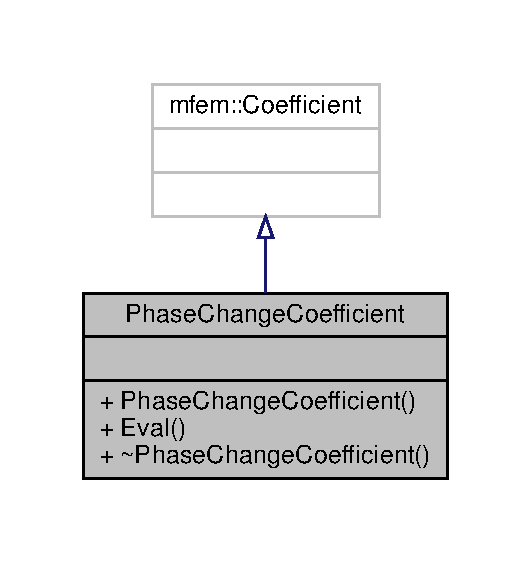
\includegraphics[width=255pt]{classPhaseChangeCoefficient__inherit__graph}
\end{center}
\end{figure}


Collaboration diagram for Phase\+Change\+Coefficient\+:\nopagebreak
\begin{figure}[H]
\begin{center}
\leavevmode
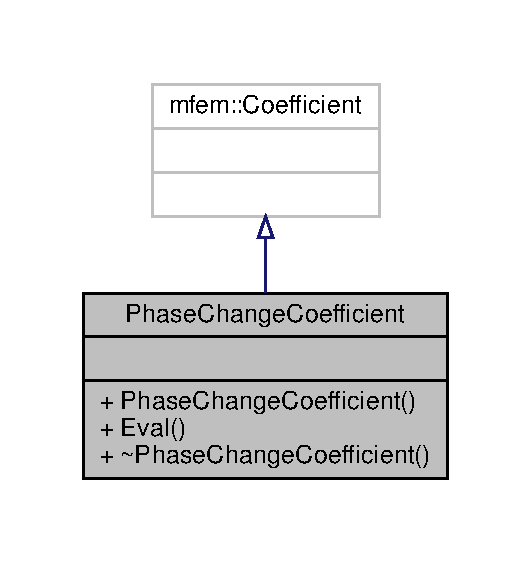
\includegraphics[width=255pt]{classPhaseChangeCoefficient__coll__graph}
\end{center}
\end{figure}
\subsection*{Public Member Functions}
\begin{DoxyCompactItemize}
\item 
\hyperlink{classPhaseChangeCoefficient_aa2c0bf141fb3d05a68522642127f867b}{Phase\+Change\+Coefficient} ()
\begin{DoxyCompactList}\small\item\em Construct a new Phase\+Change Coefficient\+:\+: Source Term Coefficient object. \end{DoxyCompactList}\item 
\mbox{\Hypertarget{classPhaseChangeCoefficient_a9c64da756fbff9bd786cfaf223eaba50}\label{classPhaseChangeCoefficient_a9c64da756fbff9bd786cfaf223eaba50}} 
double {\bfseries Eval} (mfem\+::\+Element\+Transformation \&T, const mfem\+::\+Integration\+Point \&ip)
\item 
\hyperlink{classPhaseChangeCoefficient_a3e28051637e778e8dc2b6d1a907b59ea}{$\sim$\+Phase\+Change\+Coefficient} ()
\begin{DoxyCompactList}\small\item\em Destroy the Phase Change Coefficient\+:\+: Phase Change Coefficient object. \end{DoxyCompactList}\end{DoxyCompactItemize}


\subsection{Detailed Description}


Definition at line 16 of file Phase\+Change\+Coefficient.\+hpp.



\subsection{Constructor \& Destructor Documentation}
\mbox{\Hypertarget{classPhaseChangeCoefficient_aa2c0bf141fb3d05a68522642127f867b}\label{classPhaseChangeCoefficient_aa2c0bf141fb3d05a68522642127f867b}} 
\index{Phase\+Change\+Coefficient@{Phase\+Change\+Coefficient}!Phase\+Change\+Coefficient@{Phase\+Change\+Coefficient}}
\index{Phase\+Change\+Coefficient@{Phase\+Change\+Coefficient}!Phase\+Change\+Coefficient@{Phase\+Change\+Coefficient}}
\subsubsection{\texorpdfstring{Phase\+Change\+Coefficient()}{PhaseChangeCoefficient()}}
{\footnotesize\ttfamily Phase\+Change\+Coefficient\+::\+Phase\+Change\+Coefficient (\begin{DoxyParamCaption}{ }\end{DoxyParamCaption})}



Construct a new Phase\+Change Coefficient\+:\+: Source Term Coefficient object. 


\begin{DoxyTemplParams}{Template Parameters}
{\em P\+H\+A\+SE} & \\
\hline
\end{DoxyTemplParams}


Definition at line 39 of file Phase\+Change\+Coefficient.\+hpp.


\begin{DoxyCode}
39 \{\}
\end{DoxyCode}
\mbox{\Hypertarget{classPhaseChangeCoefficient_a3e28051637e778e8dc2b6d1a907b59ea}\label{classPhaseChangeCoefficient_a3e28051637e778e8dc2b6d1a907b59ea}} 
\index{Phase\+Change\+Coefficient@{Phase\+Change\+Coefficient}!````~Phase\+Change\+Coefficient@{$\sim$\+Phase\+Change\+Coefficient}}
\index{````~Phase\+Change\+Coefficient@{$\sim$\+Phase\+Change\+Coefficient}!Phase\+Change\+Coefficient@{Phase\+Change\+Coefficient}}
\subsubsection{\texorpdfstring{$\sim$\+Phase\+Change\+Coefficient()}{~PhaseChangeCoefficient()}}
{\footnotesize\ttfamily Phase\+Change\+Coefficient\+::$\sim$\+Phase\+Change\+Coefficient (\begin{DoxyParamCaption}{ }\end{DoxyParamCaption})}



Destroy the Phase Change Coefficient\+:\+: Phase Change Coefficient object. 


\begin{DoxyTemplParams}{Template Parameters}
{\em P\+H\+A\+SE} & \\
\hline
\end{DoxyTemplParams}


Definition at line 75 of file Phase\+Change\+Coefficient.\+hpp.


\begin{DoxyCode}
75 \{\}
\end{DoxyCode}


The documentation for this class was generated from the following file\+:\begin{DoxyCompactItemize}
\item 
Phase\+Change\+Coefficient.\+hpp\end{DoxyCompactItemize}

\hypertarget{classPhaseFieldOperator}{}\section{Phase\+Field\+Operator$<$ T, D\+IM, N\+L\+FI $>$ Class Template Reference}
\label{classPhaseFieldOperator}\index{Phase\+Field\+Operator$<$ T, D\+I\+M, N\+L\+F\+I $>$@{Phase\+Field\+Operator$<$ T, D\+I\+M, N\+L\+F\+I $>$}}


\hyperlink{classPhaseFieldOperator}{Phase\+Field\+Operator} class.  




{\ttfamily \#include $<$/home/ci230846/home-\/local/\+My\+Git\+Projects/\+C\+O\+M\+P\+O\+N\+E\+N\+T/\+P\+F-\/\+M\+F\+E\+M/\+Operators/\+Phase\+Field\+Operator.\+hpp$>$}



Inheritance diagram for Phase\+Field\+Operator$<$ T, D\+IM, N\+L\+FI $>$\+:\nopagebreak
\begin{figure}[H]
\begin{center}
\leavevmode
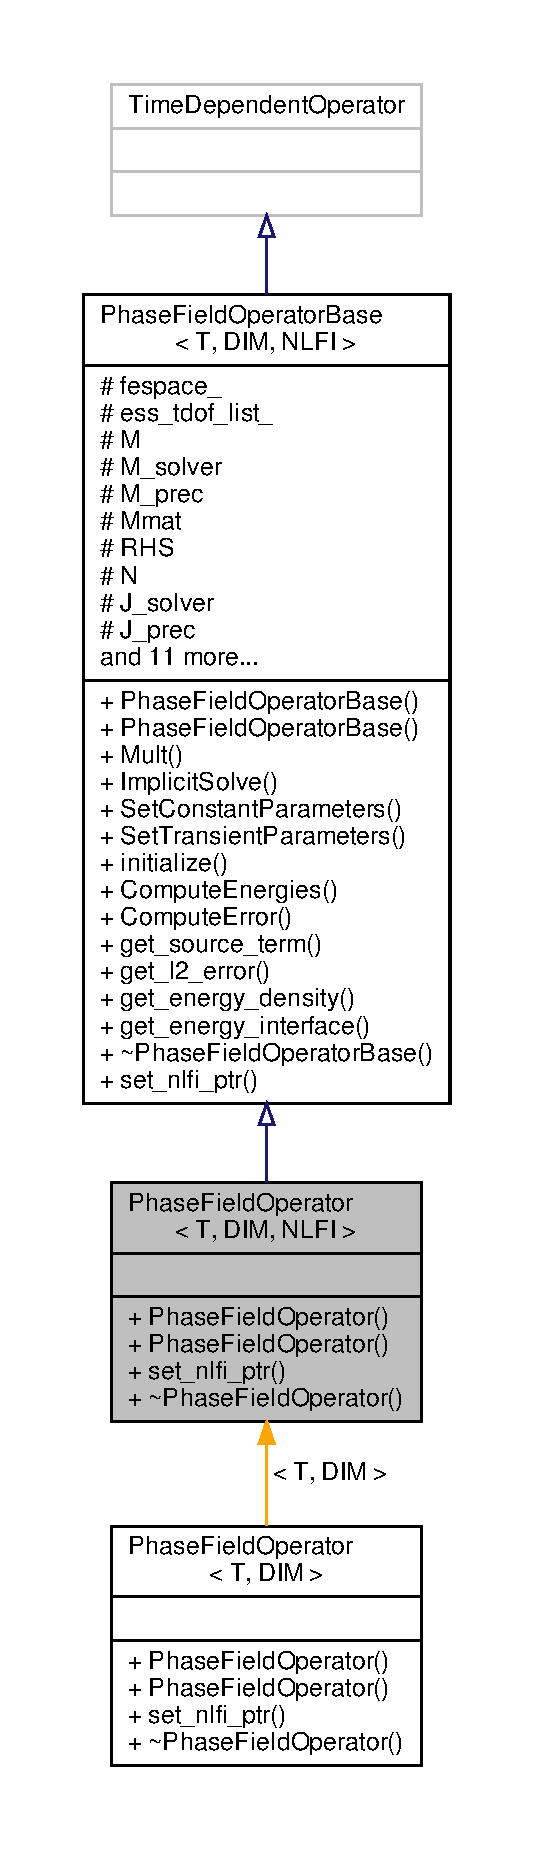
\includegraphics[height=550pt]{classPhaseFieldOperator__inherit__graph}
\end{center}
\end{figure}


Collaboration diagram for Phase\+Field\+Operator$<$ T, D\+IM, N\+L\+FI $>$\+:\nopagebreak
\begin{figure}[H]
\begin{center}
\leavevmode
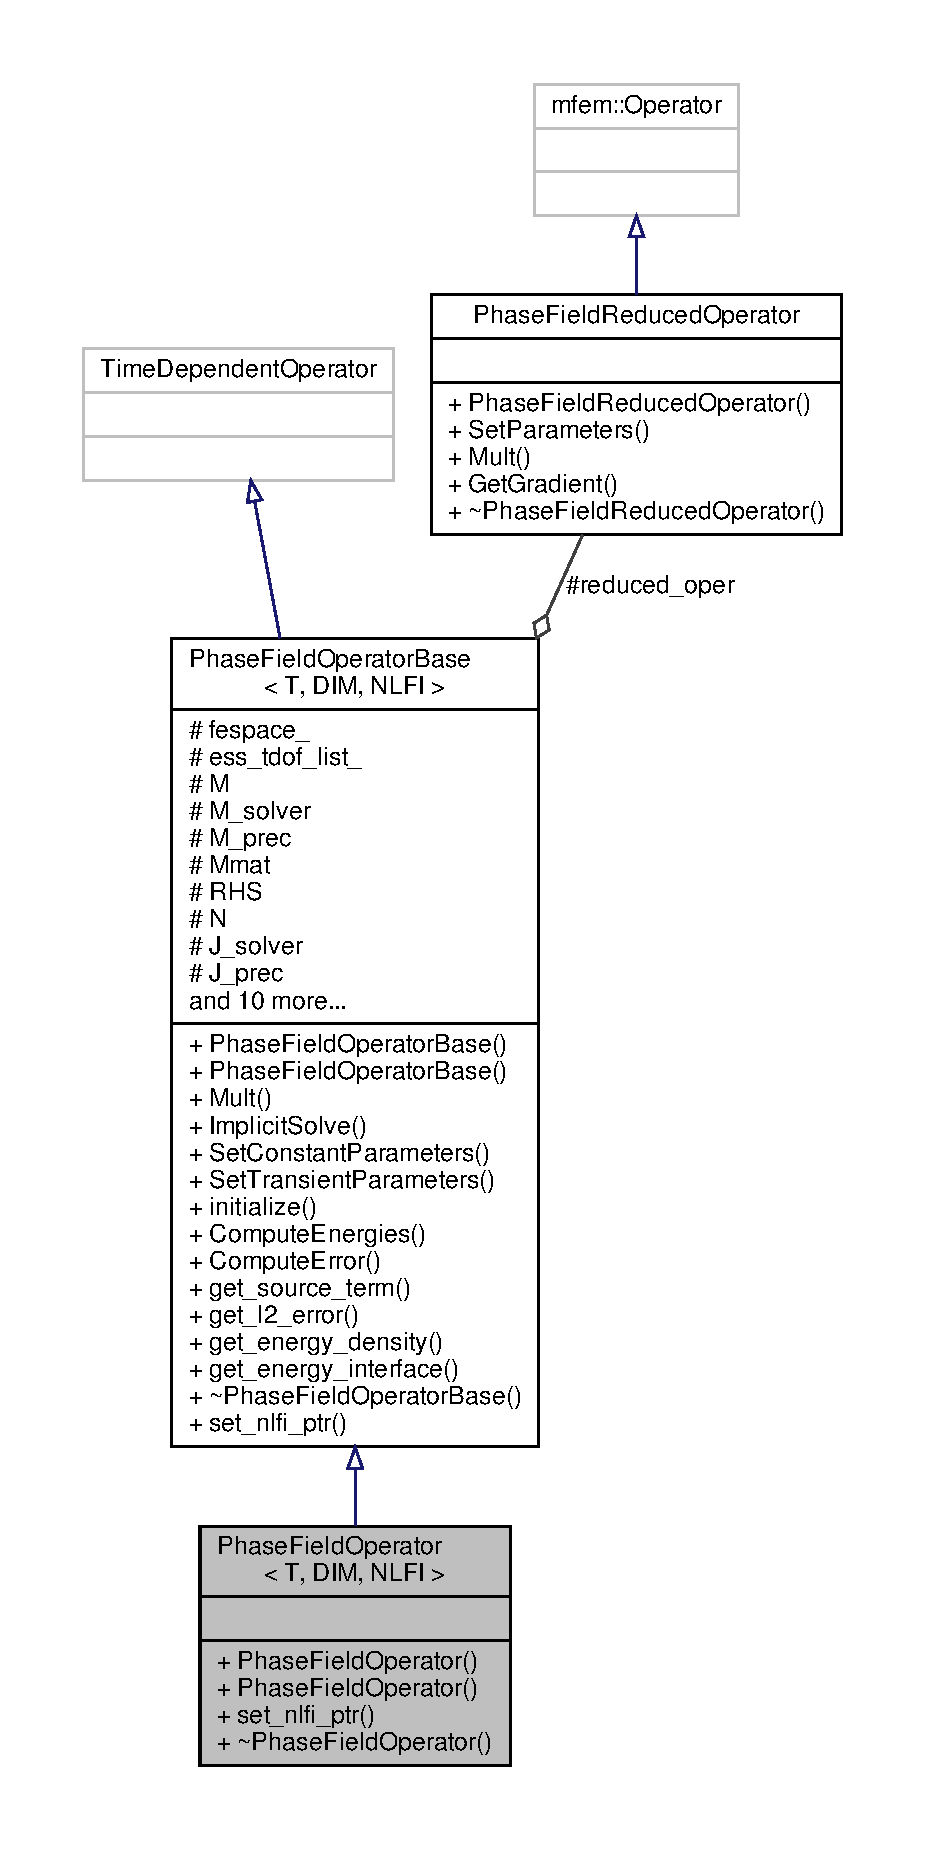
\includegraphics[height=550pt]{classPhaseFieldOperator__coll__graph}
\end{center}
\end{figure}
\subsection*{Public Member Functions}
\begin{DoxyCompactItemize}
\item 
\hyperlink{classPhaseFieldOperator_ad71bd4990d4d0098766e37a135655c1f}{Phase\+Field\+Operator} (\hyperlink{classSpatialDiscretization}{Spatial\+Discretization}$<$ T, D\+IM $>$ $\ast$spatial, const \hyperlink{classParameters}{Parameters} \&params, \hyperlink{classVariables}{Variables}$<$ T, D\+IM $>$ \&vars)
\begin{DoxyCompactList}\small\item\em Construct a new Phase Field Operator$<$ T,  D\+I\+M,  N\+L\+F\+I$>$\+:\+: Phase Field Operator object. \end{DoxyCompactList}\item 
{\footnotesize template$<$class... Args$>$ }\\\hyperlink{classPhaseFieldOperator_ad190a0a04db9daaa6f220a88a5522480}{Phase\+Field\+Operator} (\hyperlink{classSpatialDiscretization}{Spatial\+Discretization}$<$ T, D\+IM $>$ $\ast$spatial, const \hyperlink{classParameters}{Parameters} \&params, \hyperlink{classVariables}{Variables}$<$ T, D\+IM $>$ \&vars, const std\+::string \&source\+\_\+term\+\_\+name, Args... args)
\begin{DoxyCompactList}\small\item\em Construct a new Phase Field Operator$<$ T,  D\+I\+M,  N\+L\+F\+I$>$\+:\+: Phase Field Operator object. \end{DoxyCompactList}\item 
N\+L\+FI $\ast$ \hyperlink{classPhaseFieldOperator_a794471a8c45b86717f73e63e17d40ff0}{set\+\_\+nlfi\+\_\+ptr} (const double dt, const mfem\+::\+Vector \&u) override
\begin{DoxyCompactList}\small\item\em Set the Non\+Linear\+Form\+Integrator dedicated to standard phasefield calculations. \end{DoxyCompactList}\item 
virtual \hyperlink{classPhaseFieldOperator_ae22837e1962c281894631439b7029f73}{$\sim$\+Phase\+Field\+Operator} ()
\begin{DoxyCompactList}\small\item\em Destroy the Phase Field Operator Melting$<$ T,  D\+I\+M,  N\+L\+F\+I$>$\+:\+: Phase Field Operator object. \end{DoxyCompactList}\item 
virtual void \hyperlink{classPhaseFieldOperatorBase_a55a314426a0d9bbb181cb5d35e8f76e9}{Mult} (const mfem\+::\+Vector \&u, mfem\+::\+Vector \&du\+\_\+dt) const
\begin{DoxyCompactList}\small\item\em Compute the right-\/hand side of the O\+DE system. \end{DoxyCompactList}\item 
virtual void \hyperlink{classPhaseFieldOperatorBase_ac1be84d201e35ba329090cdda6a4bfc5}{Implicit\+Solve} (const double dt, const mfem\+::\+Vector \&u, mfem\+::\+Vector \&k)
\begin{DoxyCompactList}\small\item\em Solve the Backward-\/\+Euler equation\+: k = f(phi + dt$\ast$k, t), for the unknown k. \end{DoxyCompactList}\item 
void \hyperlink{classPhaseFieldOperatorBase_ae28add1cf3731d10726a9665862a725b}{Set\+Constant\+Parameters} (const double dt, mfem\+::\+Vector \&u)
\begin{DoxyCompactList}\small\item\em Set current dt, unk values -\/ needed to compute action and Jacobian. \end{DoxyCompactList}\item 
void \hyperlink{classPhaseFieldOperatorBase_a07fb8bcd8791bb712681379c160c1ad6}{Set\+Transient\+Parameters} (const double dt, const mfem\+::\+Vector \&u)
\begin{DoxyCompactList}\small\item\em Set current dt, unk values -\/ needed to compute action and Jacobian. solution\+\_\+coef. \end{DoxyCompactList}\item 
void \hyperlink{classPhaseFieldOperatorBase_a4a85f7d2ece328d8fdb8895a2b76bd0a}{initialize} (const double \&initial\+\_\+time)
\begin{DoxyCompactList}\small\item\em Initialization stage. \end{DoxyCompactList}\item 
void \hyperlink{classPhaseFieldOperatorBase_ac313363a74691d6b500191ff475b57fb}{Compute\+Energies} (const std\+::tuple$<$ int, double, double $>$ \&iter, const mfem\+::\+Vector \&u)
\begin{DoxyCompactList}\small\item\em Compute Phase-\/field Energies. \end{DoxyCompactList}\item 
void \hyperlink{classPhaseFieldOperatorBase_ae2166b96b4d740e05c5dd1ca36e9fc8c}{Compute\+Error} (const std\+::tuple$<$ int, double, double $>$ \&iter, const mfem\+::\+Vector \&u, std\+::function$<$ double(const mfem\+::\+Vector \&, double)$>$ solution\+\_\+func)
\begin{DoxyCompactList}\small\item\em Compute L2 error. \end{DoxyCompactList}\item 
void \hyperlink{classPhaseFieldOperatorBase_ade4aaf43e627fdc8b2a3690839e225d3}{get\+\_\+source\+\_\+term} (mfem\+::\+Vector \&source\+\_\+term) const
\begin{DoxyCompactList}\small\item\em get the source term \end{DoxyCompactList}\item 
const std\+::map$<$ std\+::tuple$<$ int, double, double $>$, double $>$ \hyperlink{classPhaseFieldOperatorBase_adc993d94274e82bc06f9555fbecbd310}{get\+\_\+l2\+\_\+error} () const
\begin{DoxyCompactList}\small\item\em Get a value of a map of L2 errors at a given iteration. \end{DoxyCompactList}\item 
const std\+::map$<$ std\+::tuple$<$ int, double, double $>$, double $>$ \hyperlink{classPhaseFieldOperatorBase_a8428da5d747f60f7ccbd79c879ca8d25}{get\+\_\+energy\+\_\+density} () const
\begin{DoxyCompactList}\small\item\em Get a of a map of interfacial energy at a given iteration. \end{DoxyCompactList}\item 
const std\+::map$<$ std\+::tuple$<$ int, double, double $>$, double $>$ \hyperlink{classPhaseFieldOperatorBase_ac194823660f85a12d8edcf4520bbc025}{get\+\_\+energy\+\_\+interface} () const
\begin{DoxyCompactList}\small\item\em Get a of a map of interfacial energy at a given iteration. \end{DoxyCompactList}\end{DoxyCompactItemize}
\subsection*{Protected Attributes}
\begin{DoxyCompactItemize}
\item 
\mbox{\Hypertarget{classPhaseFieldOperatorBase_ac8697ec5f9f8b2098f695403b7e7d32c}\label{classPhaseFieldOperatorBase_ac8697ec5f9f8b2098f695403b7e7d32c}} 
mfem\+::\+Finite\+Element\+Space $\ast$ {\bfseries fespace\+\_\+}
\item 
\mbox{\Hypertarget{classPhaseFieldOperatorBase_aef9d79b193e695484fc8ece8280a3c6e}\label{classPhaseFieldOperatorBase_aef9d79b193e695484fc8ece8280a3c6e}} 
mfem\+::\+Array$<$ int $>$ {\bfseries ess\+\_\+tdof\+\_\+list\+\_\+}
\item 
\mbox{\Hypertarget{classPhaseFieldOperatorBase_ac59727af25abdd5a0b0eff6a7e766ed2}\label{classPhaseFieldOperatorBase_ac59727af25abdd5a0b0eff6a7e766ed2}} 
mfem\+::\+Bilinear\+Form $\ast$ {\bfseries M}
\item 
\mbox{\Hypertarget{classPhaseFieldOperatorBase_abae6aa970af1afee541f399716c84459}\label{classPhaseFieldOperatorBase_abae6aa970af1afee541f399716c84459}} 
mfem\+::\+C\+G\+Solver {\bfseries M\+\_\+solver}
\item 
\mbox{\Hypertarget{classPhaseFieldOperatorBase_ae0ff8b7ef560d3bde9b6ba13585f57bd}\label{classPhaseFieldOperatorBase_ae0ff8b7ef560d3bde9b6ba13585f57bd}} 
mfem\+::\+D\+Smoother {\bfseries M\+\_\+prec}
\item 
\mbox{\Hypertarget{classPhaseFieldOperatorBase_a3623bbe799103af42de43d798bb3e928}\label{classPhaseFieldOperatorBase_a3623bbe799103af42de43d798bb3e928}} 
mfem\+::\+Sparse\+Matrix {\bfseries Mmat}
\item 
\mbox{\Hypertarget{classPhaseFieldOperatorBase_ab4ba4f88819f656ce8f6dddee6ded24f}\label{classPhaseFieldOperatorBase_ab4ba4f88819f656ce8f6dddee6ded24f}} 
mfem\+::\+Linear\+Form $\ast$ {\bfseries R\+HS}
\item 
\mbox{\Hypertarget{classPhaseFieldOperatorBase_a235f1d2f65754932ca9f1fbfd7f91d91}\label{classPhaseFieldOperatorBase_a235f1d2f65754932ca9f1fbfd7f91d91}} 
mfem\+::\+Nonlinear\+Form $\ast$ {\bfseries N}
\item 
\mbox{\Hypertarget{classPhaseFieldOperatorBase_af0cc6c282ae76674384e3d6a87aa88d9}\label{classPhaseFieldOperatorBase_af0cc6c282ae76674384e3d6a87aa88d9}} 
mfem\+::\+Solver $\ast$ {\bfseries J\+\_\+solver}
\item 
\mbox{\Hypertarget{classPhaseFieldOperatorBase_ab907d8e1cbd9d399959064f8fed3c3e6}\label{classPhaseFieldOperatorBase_ab907d8e1cbd9d399959064f8fed3c3e6}} 
mfem\+::\+Solver $\ast$ {\bfseries J\+\_\+prec}
\item 
\mbox{\Hypertarget{classPhaseFieldOperatorBase_ace8edd3371a4b1b1adaf22a36ad2041a}\label{classPhaseFieldOperatorBase_ace8edd3371a4b1b1adaf22a36ad2041a}} 
\hyperlink{classBoundaryConditions}{Boundary\+Conditions}$<$ T, D\+IM $>$ $\ast$ {\bfseries bcs\+\_\+}
\item 
\mbox{\Hypertarget{classPhaseFieldOperatorBase_a7613689c7c934e661ec287b7b878c9d2}\label{classPhaseFieldOperatorBase_a7613689c7c934e661ec287b7b878c9d2}} 
\hyperlink{classVariables}{Variables}$<$ T, D\+IM $>$ {\bfseries vars\+\_\+}
\item 
\mbox{\Hypertarget{classPhaseFieldOperatorBase_ae643a34ec21563a1aa1e0baee30beb30}\label{classPhaseFieldOperatorBase_ae643a34ec21563a1aa1e0baee30beb30}} 
mfem\+::\+Newton\+Solver {\bfseries newton\+\_\+solver\+\_\+}
\item 
\hyperlink{classPhaseFieldReducedOperator}{Phase\+Field\+Reduced\+Operator} $\ast$ \hyperlink{classPhaseFieldOperatorBase_a010a3da035afe945635288cc0ab2f0b5}{reduced\+\_\+oper}
\item 
\mbox{\Hypertarget{classPhaseFieldOperatorBase_aaa799d0dbf5d04e158f276cc3e0a32cc}\label{classPhaseFieldOperatorBase_aaa799d0dbf5d04e158f276cc3e0a32cc}} 
double {\bfseries mobility\+\_\+coeff\+\_\+}
\item 
\mbox{\Hypertarget{classPhaseFieldOperatorBase_a275f0cce177c9cd3c2cced2771b8f702}\label{classPhaseFieldOperatorBase_a275f0cce177c9cd3c2cced2771b8f702}} 
double {\bfseries omega\+\_\+}
\item 
\mbox{\Hypertarget{classPhaseFieldOperatorBase_a55ca706b0f6f4ee16eb1c27523569a2c}\label{classPhaseFieldOperatorBase_a55ca706b0f6f4ee16eb1c27523569a2c}} 
double {\bfseries lambda\+\_\+}
\item 
\mbox{\Hypertarget{classPhaseFieldOperatorBase_a1cc7b7915970f927c7e3bde1d06b9412}\label{classPhaseFieldOperatorBase_a1cc7b7915970f927c7e3bde1d06b9412}} 
std\+::function$<$ double(const mfem\+::\+Vector \&, double)$>$ {\bfseries src\+\_\+func\+\_\+}
\item 
\mbox{\Hypertarget{classPhaseFieldOperatorBase_ac7c9e3138a6324901705e74da62421ea}\label{classPhaseFieldOperatorBase_ac7c9e3138a6324901705e74da62421ea}} 
double {\bfseries current\+\_\+dt\+\_\+}
\item 
\mbox{\Hypertarget{classPhaseFieldOperatorBase_a67fca8849db8e5659f633a2c0df694b7}\label{classPhaseFieldOperatorBase_a67fca8849db8e5659f633a2c0df694b7}} 
mfem\+::\+Vector {\bfseries z}
\item 
\mbox{\Hypertarget{classPhaseFieldOperatorBase_aefbc006a9f535e2ab69a9a8964e2b159}\label{classPhaseFieldOperatorBase_aefbc006a9f535e2ab69a9a8964e2b159}} 
std\+::string {\bfseries source\+\_\+term\+\_\+name\+\_\+}
\end{DoxyCompactItemize}


\subsection{Detailed Description}
\subsubsection*{template$<$class T, int D\+IM, class N\+L\+FI$>$\newline
class Phase\+Field\+Operator$<$ T, D\+I\+M, N\+L\+F\+I $>$}

\hyperlink{classPhaseFieldOperator}{Phase\+Field\+Operator} class. 

Definition at line 47 of file Phase\+Field\+Operator.\+hpp.



\subsection{Constructor \& Destructor Documentation}
\mbox{\Hypertarget{classPhaseFieldOperator_ad71bd4990d4d0098766e37a135655c1f}\label{classPhaseFieldOperator_ad71bd4990d4d0098766e37a135655c1f}} 
\index{Phase\+Field\+Operator@{Phase\+Field\+Operator}!Phase\+Field\+Operator@{Phase\+Field\+Operator}}
\index{Phase\+Field\+Operator@{Phase\+Field\+Operator}!Phase\+Field\+Operator@{Phase\+Field\+Operator}}
\subsubsection{\texorpdfstring{Phase\+Field\+Operator()}{PhaseFieldOperator()}\hspace{0.1cm}{\footnotesize\ttfamily [1/2]}}
{\footnotesize\ttfamily template$<$class T, int D\+IM, class N\+L\+FI $>$ \\
\hyperlink{classPhaseFieldOperator}{Phase\+Field\+Operator}$<$ T, D\+IM, N\+L\+FI $>$\+::\hyperlink{classPhaseFieldOperator}{Phase\+Field\+Operator} (\begin{DoxyParamCaption}\item[{\hyperlink{classSpatialDiscretization}{Spatial\+Discretization}$<$ T, D\+IM $>$ $\ast$}]{spatial,  }\item[{const \hyperlink{classParameters}{Parameters} \&}]{params,  }\item[{\hyperlink{classVariables}{Variables}$<$ T, D\+IM $>$ \&}]{vars }\end{DoxyParamCaption})}



Construct a new Phase Field Operator$<$ T,  D\+I\+M,  N\+L\+F\+I$>$\+:\+: Phase Field Operator object. 


\begin{DoxyTemplParams}{Template Parameters}
{\em T} & \\
\hline
{\em D\+IM} & \\
\hline
{\em N\+L\+FI} & \\
\hline
\end{DoxyTemplParams}

\begin{DoxyParams}{Parameters}
{\em spatial} & \\
\hline
{\em params} & \\
\hline
{\em vars} & \\
\hline
\end{DoxyParams}


Definition at line 76 of file Phase\+Field\+Operator.\+hpp.


\begin{DoxyCode}
79     : \hyperlink{classPhaseFieldOperatorBase}{PhaseFieldOperatorBase<T, DIM, NLFI>}(spatial, params, vars) \{\}
\end{DoxyCode}
\mbox{\Hypertarget{classPhaseFieldOperator_ad190a0a04db9daaa6f220a88a5522480}\label{classPhaseFieldOperator_ad190a0a04db9daaa6f220a88a5522480}} 
\index{Phase\+Field\+Operator@{Phase\+Field\+Operator}!Phase\+Field\+Operator@{Phase\+Field\+Operator}}
\index{Phase\+Field\+Operator@{Phase\+Field\+Operator}!Phase\+Field\+Operator@{Phase\+Field\+Operator}}
\subsubsection{\texorpdfstring{Phase\+Field\+Operator()}{PhaseFieldOperator()}\hspace{0.1cm}{\footnotesize\ttfamily [2/2]}}
{\footnotesize\ttfamily template$<$class T, int D\+IM, class N\+L\+FI $>$ \\
template$<$class... Args$>$ \\
\hyperlink{classPhaseFieldOperator}{Phase\+Field\+Operator}$<$ T, D\+IM, N\+L\+FI $>$\+::\hyperlink{classPhaseFieldOperator}{Phase\+Field\+Operator} (\begin{DoxyParamCaption}\item[{\hyperlink{classSpatialDiscretization}{Spatial\+Discretization}$<$ T, D\+IM $>$ $\ast$}]{spatial,  }\item[{const \hyperlink{classParameters}{Parameters} \&}]{params,  }\item[{\hyperlink{classVariables}{Variables}$<$ T, D\+IM $>$ \&}]{vars,  }\item[{const std\+::string \&}]{source\+\_\+term\+\_\+name,  }\item[{Args...}]{args }\end{DoxyParamCaption})}



Construct a new Phase Field Operator$<$ T,  D\+I\+M,  N\+L\+F\+I$>$\+:\+: Phase Field Operator object. 


\begin{DoxyTemplParams}{Template Parameters}
{\em T} & \\
\hline
{\em D\+IM} & \\
\hline
{\em N\+L\+FI} & \\
\hline
\end{DoxyTemplParams}

\begin{DoxyParams}{Parameters}
{\em spatial} & \\
\hline
{\em params} & \\
\hline
{\em vars} & \\
\hline
\end{DoxyParams}


Definition at line 93 of file Phase\+Field\+Operator.\+hpp.


\begin{DoxyCode}
98     : \hyperlink{classPhaseFieldOperatorBase}{PhaseFieldOperatorBase<T, DIM, NLFI>}(spatial, params, vars, 
      source\_term\_name, args...) \{\}
\end{DoxyCode}
\mbox{\Hypertarget{classPhaseFieldOperator_ae22837e1962c281894631439b7029f73}\label{classPhaseFieldOperator_ae22837e1962c281894631439b7029f73}} 
\index{Phase\+Field\+Operator@{Phase\+Field\+Operator}!````~Phase\+Field\+Operator@{$\sim$\+Phase\+Field\+Operator}}
\index{````~Phase\+Field\+Operator@{$\sim$\+Phase\+Field\+Operator}!Phase\+Field\+Operator@{Phase\+Field\+Operator}}
\subsubsection{\texorpdfstring{$\sim$\+Phase\+Field\+Operator()}{~PhaseFieldOperator()}}
{\footnotesize\ttfamily template$<$class T , int D\+IM, class N\+L\+FI $>$ \\
\hyperlink{classPhaseFieldOperator}{Phase\+Field\+Operator}$<$ T, D\+IM, N\+L\+FI $>$\+::$\sim$\hyperlink{classPhaseFieldOperator}{Phase\+Field\+Operator} (\begin{DoxyParamCaption}{ }\end{DoxyParamCaption})\hspace{0.3cm}{\ttfamily [virtual]}}



Destroy the Phase Field Operator Melting$<$ T,  D\+I\+M,  N\+L\+F\+I$>$\+:\+: Phase Field Operator object. 


\begin{DoxyTemplParams}{Template Parameters}
{\em T} & \\
\hline
{\em D\+IM} & \\
\hline
{\em N\+L\+FI} & \\
\hline
\end{DoxyTemplParams}


Definition at line 131 of file Phase\+Field\+Operator.\+hpp.


\begin{DoxyCode}
131 \{\}
\end{DoxyCode}


\subsection{Member Function Documentation}
\mbox{\Hypertarget{classPhaseFieldOperatorBase_ac313363a74691d6b500191ff475b57fb}\label{classPhaseFieldOperatorBase_ac313363a74691d6b500191ff475b57fb}} 
\index{Phase\+Field\+Operator@{Phase\+Field\+Operator}!Compute\+Energies@{Compute\+Energies}}
\index{Compute\+Energies@{Compute\+Energies}!Phase\+Field\+Operator@{Phase\+Field\+Operator}}
\subsubsection{\texorpdfstring{Compute\+Energies()}{ComputeEnergies()}}
{\footnotesize\ttfamily template$<$class T , int D\+IM, class N\+L\+FI $>$ \\
void \hyperlink{classPhaseFieldOperatorBase}{Phase\+Field\+Operator\+Base}$<$ T, D\+IM, N\+L\+FI $>$\+::Compute\+Energies (\begin{DoxyParamCaption}\item[{const std\+::tuple$<$ int, double, double $>$ \&}]{iter,  }\item[{const mfem\+::\+Vector \&}]{u }\end{DoxyParamCaption})\hspace{0.3cm}{\ttfamily [inherited]}}



Compute Phase-\/field Energies. 


\begin{DoxyParams}{Parameters}
{\em u} & unknown vector \\
\hline
\end{DoxyParams}
\begin{DoxyReturn}{Returns}
const double 
\end{DoxyReturn}


Definition at line 338 of file Phase\+Field\+Operator\+Base.\+hpp.


\begin{DoxyCode}
339                                                                     \{
340   mfem::GridFunction un\_gf(this->fespace\_);
341   un\_gf.SetFromTrueDofs(u);
342   mfem::GridFunction gf(this->fespace\_);
343   \hyperlink{classEnergyCoefficient}{EnergyCoefficient} g(&un\_gf, 0.5 * this->lambda\_, this->omega\_);
344   gf.ProjectCoefficient(g);
345   mfem::GridFunction sigf(this->fespace\_);
346   \hyperlink{classEnergyCoefficient}{EnergyCoefficient} sig(&un\_gf, this->lambda\_, 0.);
347   sigf.ProjectCoefficient(sig);
348 
349   \textcolor{comment}{// Calcul de l'intégrale de l'objet FunctionCoefficient sur le domaine}
350   mfem::ConstantCoefficient zero(0.);
351   \textcolor{keyword}{const} \textcolor{keyword}{auto} energy = gf.ComputeL1Error(zero);
352   this->energy\_density\_.try\_emplace(iter, energy);
353   \textcolor{keyword}{const} \textcolor{keyword}{auto} interfacial\_energy = sigf.ComputeL1Error(zero);
354   this->energy\_interface\_.try\_emplace(iter, interfacial\_energy);
355 \}
\end{DoxyCode}
\mbox{\Hypertarget{classPhaseFieldOperatorBase_ae2166b96b4d740e05c5dd1ca36e9fc8c}\label{classPhaseFieldOperatorBase_ae2166b96b4d740e05c5dd1ca36e9fc8c}} 
\index{Phase\+Field\+Operator@{Phase\+Field\+Operator}!Compute\+Error@{Compute\+Error}}
\index{Compute\+Error@{Compute\+Error}!Phase\+Field\+Operator@{Phase\+Field\+Operator}}
\subsubsection{\texorpdfstring{Compute\+Error()}{ComputeError()}}
{\footnotesize\ttfamily template$<$class T , int D\+IM, class N\+L\+FI $>$ \\
void \hyperlink{classPhaseFieldOperatorBase}{Phase\+Field\+Operator\+Base}$<$ T, D\+IM, N\+L\+FI $>$\+::Compute\+Error (\begin{DoxyParamCaption}\item[{const std\+::tuple$<$ int, double, double $>$ \&}]{iter,  }\item[{const mfem\+::\+Vector \&}]{u,  }\item[{std\+::function$<$ double(const mfem\+::\+Vector \&, double)$>$}]{solution\+\_\+func }\end{DoxyParamCaption})\hspace{0.3cm}{\ttfamily [inherited]}}



Compute L2 error. 


\begin{DoxyParams}{Parameters}
{\em u} & unknown vector \\
\hline
\end{DoxyParams}
\begin{DoxyReturn}{Returns}
const double 
\end{DoxyReturn}


Definition at line 364 of file Phase\+Field\+Operator\+Base.\+hpp.


\begin{DoxyCode}
366                                                                    \{
367   mfem::GridFunction gf(this->fespace\_);
368   gf.SetFromTrueDofs(u);
369   mfem::FunctionCoefficient solution\_coef(solution\_func);
370   solution\_coef.SetTime(this->GetTime());
371   \textcolor{keyword}{const} \textcolor{keyword}{auto} error = gf.ComputeL2Error(solution\_coef);
372   this->error\_l2\_.try\_emplace(iter, error);
373 \}
\end{DoxyCode}
\mbox{\Hypertarget{classPhaseFieldOperatorBase_a8428da5d747f60f7ccbd79c879ca8d25}\label{classPhaseFieldOperatorBase_a8428da5d747f60f7ccbd79c879ca8d25}} 
\index{Phase\+Field\+Operator@{Phase\+Field\+Operator}!get\+\_\+energy\+\_\+density@{get\+\_\+energy\+\_\+density}}
\index{get\+\_\+energy\+\_\+density@{get\+\_\+energy\+\_\+density}!Phase\+Field\+Operator@{Phase\+Field\+Operator}}
\subsubsection{\texorpdfstring{get\+\_\+energy\+\_\+density()}{get\_energy\_density()}}
{\footnotesize\ttfamily template$<$class T , int D\+IM, class N\+L\+FI $>$ \\
const std\+::map$<$ std\+::tuple$<$ int, double, double $>$, double $>$ \hyperlink{classPhaseFieldOperatorBase}{Phase\+Field\+Operator\+Base}$<$ T, D\+IM, N\+L\+FI $>$\+::get\+\_\+energy\+\_\+density (\begin{DoxyParamCaption}{ }\end{DoxyParamCaption}) const\hspace{0.3cm}{\ttfamily [inherited]}}



Get a of a map of interfacial energy at a given iteration. 


\begin{DoxyTemplParams}{Template Parameters}
{\em T} & \\
\hline
{\em D\+IM} & \\
\hline
{\em N\+L\+FI} & \\
\hline
\end{DoxyTemplParams}
\begin{DoxyReturn}{Returns}
const std\+::map$<$std\+::tuple$<$int, double, double$>$, double$>$ 
\end{DoxyReturn}


Definition at line 417 of file Phase\+Field\+Operator\+Base.\+hpp.


\begin{DoxyCode}
417                                                                \{
418   \textcolor{keywordflow}{return} this->energy\_density\_;
419 \}
\end{DoxyCode}
\mbox{\Hypertarget{classPhaseFieldOperatorBase_ac194823660f85a12d8edcf4520bbc025}\label{classPhaseFieldOperatorBase_ac194823660f85a12d8edcf4520bbc025}} 
\index{Phase\+Field\+Operator@{Phase\+Field\+Operator}!get\+\_\+energy\+\_\+interface@{get\+\_\+energy\+\_\+interface}}
\index{get\+\_\+energy\+\_\+interface@{get\+\_\+energy\+\_\+interface}!Phase\+Field\+Operator@{Phase\+Field\+Operator}}
\subsubsection{\texorpdfstring{get\+\_\+energy\+\_\+interface()}{get\_energy\_interface()}}
{\footnotesize\ttfamily template$<$class T , int D\+IM, class N\+L\+FI $>$ \\
const std\+::map$<$ std\+::tuple$<$ int, double, double $>$, double $>$ \hyperlink{classPhaseFieldOperatorBase}{Phase\+Field\+Operator\+Base}$<$ T, D\+IM, N\+L\+FI $>$\+::get\+\_\+energy\+\_\+interface (\begin{DoxyParamCaption}{ }\end{DoxyParamCaption}) const\hspace{0.3cm}{\ttfamily [inherited]}}



Get a of a map of interfacial energy at a given iteration. 


\begin{DoxyTemplParams}{Template Parameters}
{\em T} & \\
\hline
{\em D\+IM} & \\
\hline
{\em N\+L\+FI} & \\
\hline
\end{DoxyTemplParams}
\begin{DoxyReturn}{Returns}
const std\+::map$<$std\+::tuple$<$int, double, double$>$, double$>$ 
\end{DoxyReturn}


Definition at line 431 of file Phase\+Field\+Operator\+Base.\+hpp.


\begin{DoxyCode}
431                                                                  \{
432   \textcolor{keywordflow}{return} this->energy\_interface\_;
433 \}
\end{DoxyCode}
\mbox{\Hypertarget{classPhaseFieldOperatorBase_adc993d94274e82bc06f9555fbecbd310}\label{classPhaseFieldOperatorBase_adc993d94274e82bc06f9555fbecbd310}} 
\index{Phase\+Field\+Operator@{Phase\+Field\+Operator}!get\+\_\+l2\+\_\+error@{get\+\_\+l2\+\_\+error}}
\index{get\+\_\+l2\+\_\+error@{get\+\_\+l2\+\_\+error}!Phase\+Field\+Operator@{Phase\+Field\+Operator}}
\subsubsection{\texorpdfstring{get\+\_\+l2\+\_\+error()}{get\_l2\_error()}}
{\footnotesize\ttfamily template$<$class T , int D\+IM, class N\+L\+FI $>$ \\
const std\+::map$<$ std\+::tuple$<$ int, double, double $>$, double $>$ \hyperlink{classPhaseFieldOperatorBase}{Phase\+Field\+Operator\+Base}$<$ T, D\+IM, N\+L\+FI $>$\+::get\+\_\+l2\+\_\+error (\begin{DoxyParamCaption}{ }\end{DoxyParamCaption}) const\hspace{0.3cm}{\ttfamily [inherited]}}



Get a value of a map of L2 errors at a given iteration. 


\begin{DoxyTemplParams}{Template Parameters}
{\em T} & \\
\hline
{\em D\+IM} & \\
\hline
{\em N\+L\+FI} & \\
\hline
\end{DoxyTemplParams}

\begin{DoxyParams}{Parameters}
{\em iter} & \\
\hline
\end{DoxyParams}
\begin{DoxyReturn}{Returns}
const std\+::map$<$std\+::tuple$<$int, double, double$>$, double$>$ 
\end{DoxyReturn}


Definition at line 403 of file Phase\+Field\+Operator\+Base.\+hpp.


\begin{DoxyCode}
403                                                          \{
404   \textcolor{keywordflow}{return} this->error\_l2\_;
405 \}
\end{DoxyCode}
\mbox{\Hypertarget{classPhaseFieldOperatorBase_ade4aaf43e627fdc8b2a3690839e225d3}\label{classPhaseFieldOperatorBase_ade4aaf43e627fdc8b2a3690839e225d3}} 
\index{Phase\+Field\+Operator@{Phase\+Field\+Operator}!get\+\_\+source\+\_\+term@{get\+\_\+source\+\_\+term}}
\index{get\+\_\+source\+\_\+term@{get\+\_\+source\+\_\+term}!Phase\+Field\+Operator@{Phase\+Field\+Operator}}
\subsubsection{\texorpdfstring{get\+\_\+source\+\_\+term()}{get\_source\_term()}}
{\footnotesize\ttfamily template$<$class T , int D\+IM, class N\+L\+FI $>$ \\
void \hyperlink{classPhaseFieldOperatorBase}{Phase\+Field\+Operator\+Base}$<$ T, D\+IM, N\+L\+FI $>$\+::get\+\_\+source\+\_\+term (\begin{DoxyParamCaption}\item[{mfem\+::\+Vector \&}]{source\+\_\+term }\end{DoxyParamCaption}) const\hspace{0.3cm}{\ttfamily [inherited]}}



get the source term 


\begin{DoxyTemplParams}{Template Parameters}
{\em T} & \\
\hline
{\em D\+IM} & \\
\hline
{\em N\+L\+FI} & \\
\hline
\end{DoxyTemplParams}


Definition at line 383 of file Phase\+Field\+Operator\+Base.\+hpp.



Referenced by Phase\+Field\+Operator\+Base$<$ T, D\+I\+M, N\+L\+F\+I $>$\+::\+Implicit\+Solve(), and Phase\+Field\+Operator\+Base$<$ T, D\+I\+M, N\+L\+F\+I $>$\+::\+Mult().


\begin{DoxyCode}
383                                                                                         \{
384   std::shared\_ptr<mfem::LinearForm> RHSS(\textcolor{keyword}{new} mfem::LinearForm(this->fespace\_));
385   mfem::FunctionCoefficient src(this->src\_func\_);
386   src.SetTime(this->GetTime());
387   RHSS->AddDomainIntegrator(\textcolor{keyword}{new} mfem::DomainLFIntegrator(src));
388   RHSS->Assemble();
389   source\_term = *RHSS.get();
390 \}
\end{DoxyCode}
\mbox{\Hypertarget{classPhaseFieldOperatorBase_ac1be84d201e35ba329090cdda6a4bfc5}\label{classPhaseFieldOperatorBase_ac1be84d201e35ba329090cdda6a4bfc5}} 
\index{Phase\+Field\+Operator@{Phase\+Field\+Operator}!Implicit\+Solve@{Implicit\+Solve}}
\index{Implicit\+Solve@{Implicit\+Solve}!Phase\+Field\+Operator@{Phase\+Field\+Operator}}
\subsubsection{\texorpdfstring{Implicit\+Solve()}{ImplicitSolve()}}
{\footnotesize\ttfamily template$<$class T , int D\+IM, class N\+L\+FI $>$ \\
void \hyperlink{classPhaseFieldOperatorBase}{Phase\+Field\+Operator\+Base}$<$ T, D\+IM, N\+L\+FI $>$\+::Implicit\+Solve (\begin{DoxyParamCaption}\item[{const double}]{dt,  }\item[{const mfem\+::\+Vector \&}]{u,  }\item[{mfem\+::\+Vector \&}]{du\+\_\+dt }\end{DoxyParamCaption})\hspace{0.3cm}{\ttfamily [virtual]}, {\ttfamily [inherited]}}



Solve the Backward-\/\+Euler equation\+: k = f(phi + dt$\ast$k, t), for the unknown k. 

Solve the Backward-\/\+Euler equation\+: k = f(u + dt$\ast$k, t), for the unknown k. This is the only requirement for high-\/order S\+D\+I\+RK implicit integration.


\begin{DoxyParams}{Parameters}
{\em dt} & current time step \\
\hline
{\em u} & unknown vector \\
\hline
{\em du\+\_\+dt} & unkwon time derivative vector \\
\hline
\end{DoxyParams}


Definition at line 302 of file Phase\+Field\+Operator\+Base.\+hpp.



References Phase\+Field\+Operator\+Base$<$ T, D\+I\+M, N\+L\+F\+I $>$\+::get\+\_\+source\+\_\+term(), Boundary\+Conditions$<$ T, D\+I\+M $>$\+::\+Set\+Boundary\+Conditions(), Phase\+Field\+Reduced\+Operator\+::\+Set\+Parameters(), and Phase\+Field\+Operator\+Base$<$ T, D\+I\+M, N\+L\+F\+I $>$\+::\+Set\+Transient\+Parameters().


\begin{DoxyCode}
303                                                                             \{
304   \textcolor{keyword}{const} \textcolor{keyword}{auto} sc = height;
305   mfem::Vector v(u.GetData(), sc);
306   mfem::Vector dv\_dt(du\_dt.GetData(), sc);
307   \textcolor{comment}{// // Solve the equation:}
308   \textcolor{comment}{// //    du\_dt = M^\{-1\}*[-K(u + dt*du\_dt)]}
309   \textcolor{comment}{// // for du\_dt}
310 
311   this->bcs\_->SetBoundaryConditions(v);
312   this->\hyperlink{classPhaseFieldOperatorBase_a07fb8bcd8791bb712681379c160c1ad6}{SetTransientParameters}(dt, v);
313 
314   \hyperlink{classPhaseFieldOperatorBase_a010a3da035afe945635288cc0ab2f0b5}{reduced\_oper}->\hyperlink{classPhaseFieldReducedOperator_aaaa55d33260a9dc98051bd97f916bf46}{SetParameters}(dt, &v);
315 
316   \textcolor{comment}{// Source term}
317   mfem::Vector source\_term;
318   \textcolor{keywordflow}{if} (!this->source\_term\_name\_.empty()) \{
319     this->\hyperlink{classPhaseFieldOperatorBase_ade4aaf43e627fdc8b2a3690839e225d3}{get\_source\_term}(source\_term);
320   \}
321 
322   dv\_dt = v;
323   dv\_dt *= (1. / dt);
324   this->newton\_solver\_.Mult(source\_term, dv\_dt);
325   dv\_dt.SetSubVector(this->ess\_tdof\_list\_, 0.0);  \textcolor{comment}{// pour  Dirichlet ... uniquement?}
326   \textcolor{comment}{// std::cout << " PhaseFieldOperatorBase this->newton\_solver\_->Mult " << std::endl;}
327 
328   MFEM\_VERIFY(this->newton\_solver\_.GetConverged(), \textcolor{stringliteral}{"Nonlinear solver did not converge."});
329 \}
\end{DoxyCode}
\mbox{\Hypertarget{classPhaseFieldOperatorBase_a4a85f7d2ece328d8fdb8895a2b76bd0a}\label{classPhaseFieldOperatorBase_a4a85f7d2ece328d8fdb8895a2b76bd0a}} 
\index{Phase\+Field\+Operator@{Phase\+Field\+Operator}!initialize@{initialize}}
\index{initialize@{initialize}!Phase\+Field\+Operator@{Phase\+Field\+Operator}}
\subsubsection{\texorpdfstring{initialize()}{initialize()}}
{\footnotesize\ttfamily template$<$class T , int D\+IM, class N\+L\+FI $>$ \\
void \hyperlink{classPhaseFieldOperatorBase}{Phase\+Field\+Operator\+Base}$<$ T, D\+IM, N\+L\+FI $>$\+::initialize (\begin{DoxyParamCaption}\item[{const double \&}]{initial\+\_\+time }\end{DoxyParamCaption})\hspace{0.3cm}{\ttfamily [inherited]}}



Initialization stage. 


\begin{DoxyParams}{Parameters}
{\em vv} & \\
\hline
\end{DoxyParams}


Definition at line 186 of file Phase\+Field\+Operator\+Base.\+hpp.



References Variables$<$ T, D\+I\+M $>$\+::get\+\_\+variable(), Boundary\+Conditions$<$ T, D\+I\+M $>$\+::\+Get\+Essential\+Dofs(), Boundary\+Conditions$<$ T, D\+I\+M $>$\+::\+Set\+Boundary\+Conditions(), Phase\+Field\+Operator\+Base$<$ T, D\+I\+M, N\+L\+F\+I $>$\+::\+Set\+Constant\+Parameters(), and Phase\+Field\+Operator\+Base$<$ T, D\+I\+M, N\+L\+F\+I $>$\+::\+Set\+Transient\+Parameters().


\begin{DoxyCode}
186                                                                                 \{
187   this->SetTime(initial\_time);
188   \textcolor{keyword}{auto} &vv = vars\_.get\_variable(\textcolor{stringliteral}{"phi"});
189   \textcolor{keyword}{auto} u = vv.get\_unknown();
190 
191   this->bcs\_ = vv.get\_boundary\_conditions();
192   this->ess\_tdof\_list\_ = this->bcs\_->GetEssentialDofs();
193   this->bcs\_->SetBoundaryConditions(u);
194   this->\hyperlink{classPhaseFieldOperatorBase_ae28add1cf3731d10726a9665862a725b}{SetConstantParameters}(this->current\_dt\_, u);
195   this->\hyperlink{classPhaseFieldOperatorBase_a07fb8bcd8791bb712681379c160c1ad6}{SetTransientParameters}(this->current\_dt\_, u);
196   vv.update(u);
197 \}
\end{DoxyCode}
\mbox{\Hypertarget{classPhaseFieldOperatorBase_a55a314426a0d9bbb181cb5d35e8f76e9}\label{classPhaseFieldOperatorBase_a55a314426a0d9bbb181cb5d35e8f76e9}} 
\index{Phase\+Field\+Operator@{Phase\+Field\+Operator}!Mult@{Mult}}
\index{Mult@{Mult}!Phase\+Field\+Operator@{Phase\+Field\+Operator}}
\subsubsection{\texorpdfstring{Mult()}{Mult()}}
{\footnotesize\ttfamily template$<$class T , int D\+IM, class N\+L\+FI $>$ \\
void \hyperlink{classPhaseFieldOperatorBase}{Phase\+Field\+Operator\+Base}$<$ T, D\+IM, N\+L\+FI $>$\+::Mult (\begin{DoxyParamCaption}\item[{const mfem\+::\+Vector \&}]{u,  }\item[{mfem\+::\+Vector \&}]{du\+\_\+dt }\end{DoxyParamCaption}) const\hspace{0.3cm}{\ttfamily [virtual]}, {\ttfamily [inherited]}}



Compute the right-\/hand side of the O\+DE system. 


\begin{DoxyParams}{Parameters}
{\em u} & unknown vector \\
\hline
{\em du\+\_\+dt} & unkwon time derivative vector \\
\hline
\end{DoxyParams}


Definition at line 276 of file Phase\+Field\+Operator\+Base.\+hpp.



References Phase\+Field\+Operator\+Base$<$ T, D\+I\+M, N\+L\+F\+I $>$\+::get\+\_\+source\+\_\+term().


\begin{DoxyCode}
276                                                                                             \{
277   \textcolor{keyword}{const} \textcolor{keyword}{auto} sc = height;
278   mfem::Vector v(u.GetData(), sc);
279   mfem::Vector dv\_dt(du\_dt.GetData(), sc);
280 
281   N->Mult(v, z);
282 
283   \textcolor{comment}{// Source term}
284   \textcolor{keywordflow}{if} (!this->source\_term\_name\_.empty()) \{
285     mfem::Vector source\_term;
286     this->\hyperlink{classPhaseFieldOperatorBase_ade4aaf43e627fdc8b2a3690839e225d3}{get\_source\_term}(source\_term);
287     z -= source\_term;
288   \}
289 
290   z.Neg();  \textcolor{comment}{// z = -z}
291   M\_solver.Mult(z, dv\_dt);
292 \}
\end{DoxyCode}
\mbox{\Hypertarget{classPhaseFieldOperator_a794471a8c45b86717f73e63e17d40ff0}\label{classPhaseFieldOperator_a794471a8c45b86717f73e63e17d40ff0}} 
\index{Phase\+Field\+Operator@{Phase\+Field\+Operator}!set\+\_\+nlfi\+\_\+ptr@{set\+\_\+nlfi\+\_\+ptr}}
\index{set\+\_\+nlfi\+\_\+ptr@{set\+\_\+nlfi\+\_\+ptr}!Phase\+Field\+Operator@{Phase\+Field\+Operator}}
\subsubsection{\texorpdfstring{set\+\_\+nlfi\+\_\+ptr()}{set\_nlfi\_ptr()}}
{\footnotesize\ttfamily template$<$class T , int D\+IM, class N\+L\+FI $>$ \\
N\+L\+FI $\ast$ \hyperlink{classPhaseFieldOperator}{Phase\+Field\+Operator}$<$ T, D\+IM, N\+L\+FI $>$\+::set\+\_\+nlfi\+\_\+ptr (\begin{DoxyParamCaption}\item[{const double}]{dt,  }\item[{const mfem\+::\+Vector \&}]{u }\end{DoxyParamCaption})\hspace{0.3cm}{\ttfamily [override]}, {\ttfamily [virtual]}}



Set the Non\+Linear\+Form\+Integrator dedicated to standard phasefield calculations. 


\begin{DoxyTemplParams}{Template Parameters}
{\em T} & \\
\hline
{\em D\+IM} & \\
\hline
{\em N\+L\+FI} & \\
\hline
\end{DoxyTemplParams}

\begin{DoxyParams}{Parameters}
{\em dt} & \\
\hline
{\em u} & \\
\hline
\end{DoxyParams}
\begin{DoxyReturn}{Returns}
N\+L\+F\+I$\ast$ 
\end{DoxyReturn}


Implements \hyperlink{classPhaseFieldOperatorBase}{Phase\+Field\+Operator\+Base$<$ T, D\+I\+M, N\+L\+F\+I $>$}.



Definition at line 115 of file Phase\+Field\+Operator.\+hpp.


\begin{DoxyCode}
115                                                                                          \{
116   mfem::GridFunction un(this->fespace\_);
117   un.SetFromTrueDofs(u);
118   NLFI *nlfi\_ptr = \textcolor{keyword}{new} NLFI(un, this->omega\_, this->lambda\_, this->mobility\_coeff\_);
119   \textcolor{keywordflow}{return} nlfi\_ptr;
120 \}
\end{DoxyCode}
\mbox{\Hypertarget{classPhaseFieldOperatorBase_ae28add1cf3731d10726a9665862a725b}\label{classPhaseFieldOperatorBase_ae28add1cf3731d10726a9665862a725b}} 
\index{Phase\+Field\+Operator@{Phase\+Field\+Operator}!Set\+Constant\+Parameters@{Set\+Constant\+Parameters}}
\index{Set\+Constant\+Parameters@{Set\+Constant\+Parameters}!Phase\+Field\+Operator@{Phase\+Field\+Operator}}
\subsubsection{\texorpdfstring{Set\+Constant\+Parameters()}{SetConstantParameters()}}
{\footnotesize\ttfamily template$<$class T , int D\+IM, class N\+L\+FI $>$ \\
void \hyperlink{classPhaseFieldOperatorBase}{Phase\+Field\+Operator\+Base}$<$ T, D\+IM, N\+L\+FI $>$\+::Set\+Constant\+Parameters (\begin{DoxyParamCaption}\item[{const double}]{dt,  }\item[{mfem\+::\+Vector \&}]{u }\end{DoxyParamCaption})\hspace{0.3cm}{\ttfamily [inherited]}}



Set current dt, unk values -\/ needed to compute action and Jacobian. 


\begin{DoxyParams}{Parameters}
{\em dt} & time-\/step \\
\hline
{\em u} & unknown vector \\
\hline
{\em ess\+\_\+tdof\+\_\+list} & array of dofs \\
\hline
\end{DoxyParams}


Definition at line 250 of file Phase\+Field\+Operator\+Base.\+hpp.



References Utils\+For\+Solvers\+::\+Build\+Solver(), and Utils\+For\+Solvers\+::\+Set\+Solver\+Parameters().



Referenced by Phase\+Field\+Operator\+Base$<$ T, D\+I\+M, N\+L\+F\+I $>$\+::initialize().


\begin{DoxyCode}
250                                                                                                \{
251   \textcolor{keyword}{delete} M;
253   \textcolor{comment}{// Mass matrix (constant)}
255 \textcolor{comment}{}  M = \textcolor{keyword}{new} mfem::BilinearForm(this->fespace\_);
256   M->AddDomainIntegrator(\textcolor{keyword}{new} mfem::MassIntegrator());
257   M->Assemble(0);
258   mfem::SparseMatrix tmp;
259   M->FormSystemMatrix(this->ess\_tdof\_list\_, Mmat);
260   this->ut\_solver\_.\hyperlink{classUtilsForSolvers_a5e352c96817ea210dcf3e080c13d4b1d}{SetSolverParameters}(
261       M\_solver, MassDefaultConstant::print\_level, MassDefaultConstant::iterative\_mode,
262       MassDefaultConstant::iter\_max, MassDefaultConstant::rel\_tol, MassDefaultConstant::abs\_tol);
263   this->ut\_solver\_.\hyperlink{classUtilsForSolvers_a5c76f7ef4f28a5e22f6d07666134aa4d}{BuildSolver}(M\_solver, M\_prec, Mmat);
264 \}
\end{DoxyCode}
\mbox{\Hypertarget{classPhaseFieldOperatorBase_a07fb8bcd8791bb712681379c160c1ad6}\label{classPhaseFieldOperatorBase_a07fb8bcd8791bb712681379c160c1ad6}} 
\index{Phase\+Field\+Operator@{Phase\+Field\+Operator}!Set\+Transient\+Parameters@{Set\+Transient\+Parameters}}
\index{Set\+Transient\+Parameters@{Set\+Transient\+Parameters}!Phase\+Field\+Operator@{Phase\+Field\+Operator}}
\subsubsection{\texorpdfstring{Set\+Transient\+Parameters()}{SetTransientParameters()}}
{\footnotesize\ttfamily template$<$class T , int D\+IM, class N\+L\+FI $>$ \\
void \hyperlink{classPhaseFieldOperatorBase}{Phase\+Field\+Operator\+Base}$<$ T, D\+IM, N\+L\+FI $>$\+::Set\+Transient\+Parameters (\begin{DoxyParamCaption}\item[{const double}]{dt,  }\item[{const mfem\+::\+Vector \&}]{u }\end{DoxyParamCaption})\hspace{0.3cm}{\ttfamily [inherited]}}



Set current dt, unk values -\/ needed to compute action and Jacobian. solution\+\_\+coef. 


\begin{DoxyParams}{Parameters}
{\em dt} & time-\/step \\
\hline
{\em u} & unknown vector \\
\hline
\end{DoxyParams}


Definition at line 210 of file Phase\+Field\+Operator\+Base.\+hpp.



References Utils\+For\+Solvers\+::\+Build\+Solver(), Phase\+Field\+Operator\+Base$<$ T, D\+I\+M, N\+L\+F\+I $>$\+::reduced\+\_\+oper, and Utils\+For\+Solvers\+::\+Set\+Solver\+Parameters().



Referenced by Phase\+Field\+Operator\+Base$<$ T, D\+I\+M, N\+L\+F\+I $>$\+::\+Implicit\+Solve(), and Phase\+Field\+Operator\+Base$<$ T, D\+I\+M, N\+L\+F\+I $>$\+::initialize().


\begin{DoxyCode}
211                                                                                        \{
212   \textcolor{keyword}{delete} N;
213   \textcolor{keyword}{delete} \hyperlink{classPhaseFieldOperatorBase_a010a3da035afe945635288cc0ab2f0b5}{reduced\_oper};
214 
216   \textcolor{comment}{// PhaseField reduced operator N}
218 \textcolor{comment}{}  N = \textcolor{keyword}{new} mfem::NonlinearForm(this->fespace\_);
219   mfem::GridFunction un\_gf(this->fespace\_);
220   un\_gf.SetFromTrueDofs(u);
221   mfem::GridFunction un(this->fespace\_);
222   un.SetFromTrueDofs(u);
223 
224   NLFI *nlfi\_ptr = set\_nlfi\_ptr(dt, u);
225   N->AddDomainIntegrator(nlfi\_ptr);
226   N->SetEssentialTrueDofs(this->ess\_tdof\_list\_);
227 
228   \hyperlink{classPhaseFieldOperatorBase_a010a3da035afe945635288cc0ab2f0b5}{reduced\_oper} = \textcolor{keyword}{new} \hyperlink{classPhaseFieldReducedOperator}{PhaseFieldReducedOperator}(M, N);
229 
231   \textcolor{comment}{// Newton Solver}
233 \textcolor{comment}{}  this->ut\_solver\_.\hyperlink{classUtilsForSolvers_a5e352c96817ea210dcf3e080c13d4b1d}{SetSolverParameters}(
234       this->newton\_solver\_, NewtonDefaultConstant::print\_level,
235       NewtonDefaultConstant::iterative\_mode, NewtonDefaultConstant::iter\_max,
236       NewtonDefaultConstant::rel\_tol, NewtonDefaultConstant::abs\_tol);
237   \textcolor{comment}{// TODO(ci230846) : cette partie devra etre generalisee pour un solveur iteratif}
238   J\_solver = \textcolor{keyword}{new} mfem::UMFPackSolver;
239   this->ut\_solver\_.\hyperlink{classUtilsForSolvers_a5c76f7ef4f28a5e22f6d07666134aa4d}{BuildSolver}(this->newton\_solver\_, *J\_solver, *
      \hyperlink{classPhaseFieldOperatorBase_a010a3da035afe945635288cc0ab2f0b5}{reduced\_oper});
240 \}
\end{DoxyCode}


\subsection{Field Documentation}
\mbox{\Hypertarget{classPhaseFieldOperatorBase_a010a3da035afe945635288cc0ab2f0b5}\label{classPhaseFieldOperatorBase_a010a3da035afe945635288cc0ab2f0b5}} 
\index{Phase\+Field\+Operator@{Phase\+Field\+Operator}!reduced\+\_\+oper@{reduced\+\_\+oper}}
\index{reduced\+\_\+oper@{reduced\+\_\+oper}!Phase\+Field\+Operator@{Phase\+Field\+Operator}}
\subsubsection{\texorpdfstring{reduced\+\_\+oper}{reduced\_oper}}
{\footnotesize\ttfamily template$<$class T, int D\+IM, class N\+L\+FI$>$ \\
\hyperlink{classPhaseFieldReducedOperator}{Phase\+Field\+Reduced\+Operator}$\ast$ \hyperlink{classPhaseFieldOperatorBase}{Phase\+Field\+Operator\+Base}$<$ T, D\+IM, N\+L\+FI $>$\+::reduced\+\_\+oper\hspace{0.3cm}{\ttfamily [protected]}, {\ttfamily [inherited]}}

Nonlinear operator defining the reduced backward Euler equation for the velocity. Used in the implementation of method Implicit\+Solve. 

Definition at line 80 of file Phase\+Field\+Operator\+Base.\+hpp.



Referenced by Phase\+Field\+Operator\+Base$<$ T, D\+I\+M, N\+L\+F\+I $>$\+::\+Set\+Transient\+Parameters().



The documentation for this class was generated from the following file\+:\begin{DoxyCompactItemize}
\item 
Phase\+Field\+Operator.\+hpp\end{DoxyCompactItemize}

\hypertarget{classPhaseFieldOperatorBase}{}\section{Phase\+Field\+Operator\+Base$<$ T, D\+IM, N\+L\+FI $>$ Class Template Reference}
\label{classPhaseFieldOperatorBase}\index{Phase\+Field\+Operator\+Base$<$ T, D\+I\+M, N\+L\+F\+I $>$@{Phase\+Field\+Operator\+Base$<$ T, D\+I\+M, N\+L\+F\+I $>$}}


\hyperlink{classPhaseFieldOperatorBase}{Phase\+Field\+Operator\+Base} class.  




{\ttfamily \#include $<$/home/ci230846/home-\/local/\+My\+Git\+Projects/\+C\+O\+M\+P\+O\+N\+E\+N\+T/\+P\+F-\/\+M\+F\+E\+M/\+Operators/\+Phase\+Field\+Operator\+Base.\+hpp$>$}



Inheritance diagram for Phase\+Field\+Operator\+Base$<$ T, D\+IM, N\+L\+FI $>$\+:\nopagebreak
\begin{figure}[H]
\begin{center}
\leavevmode
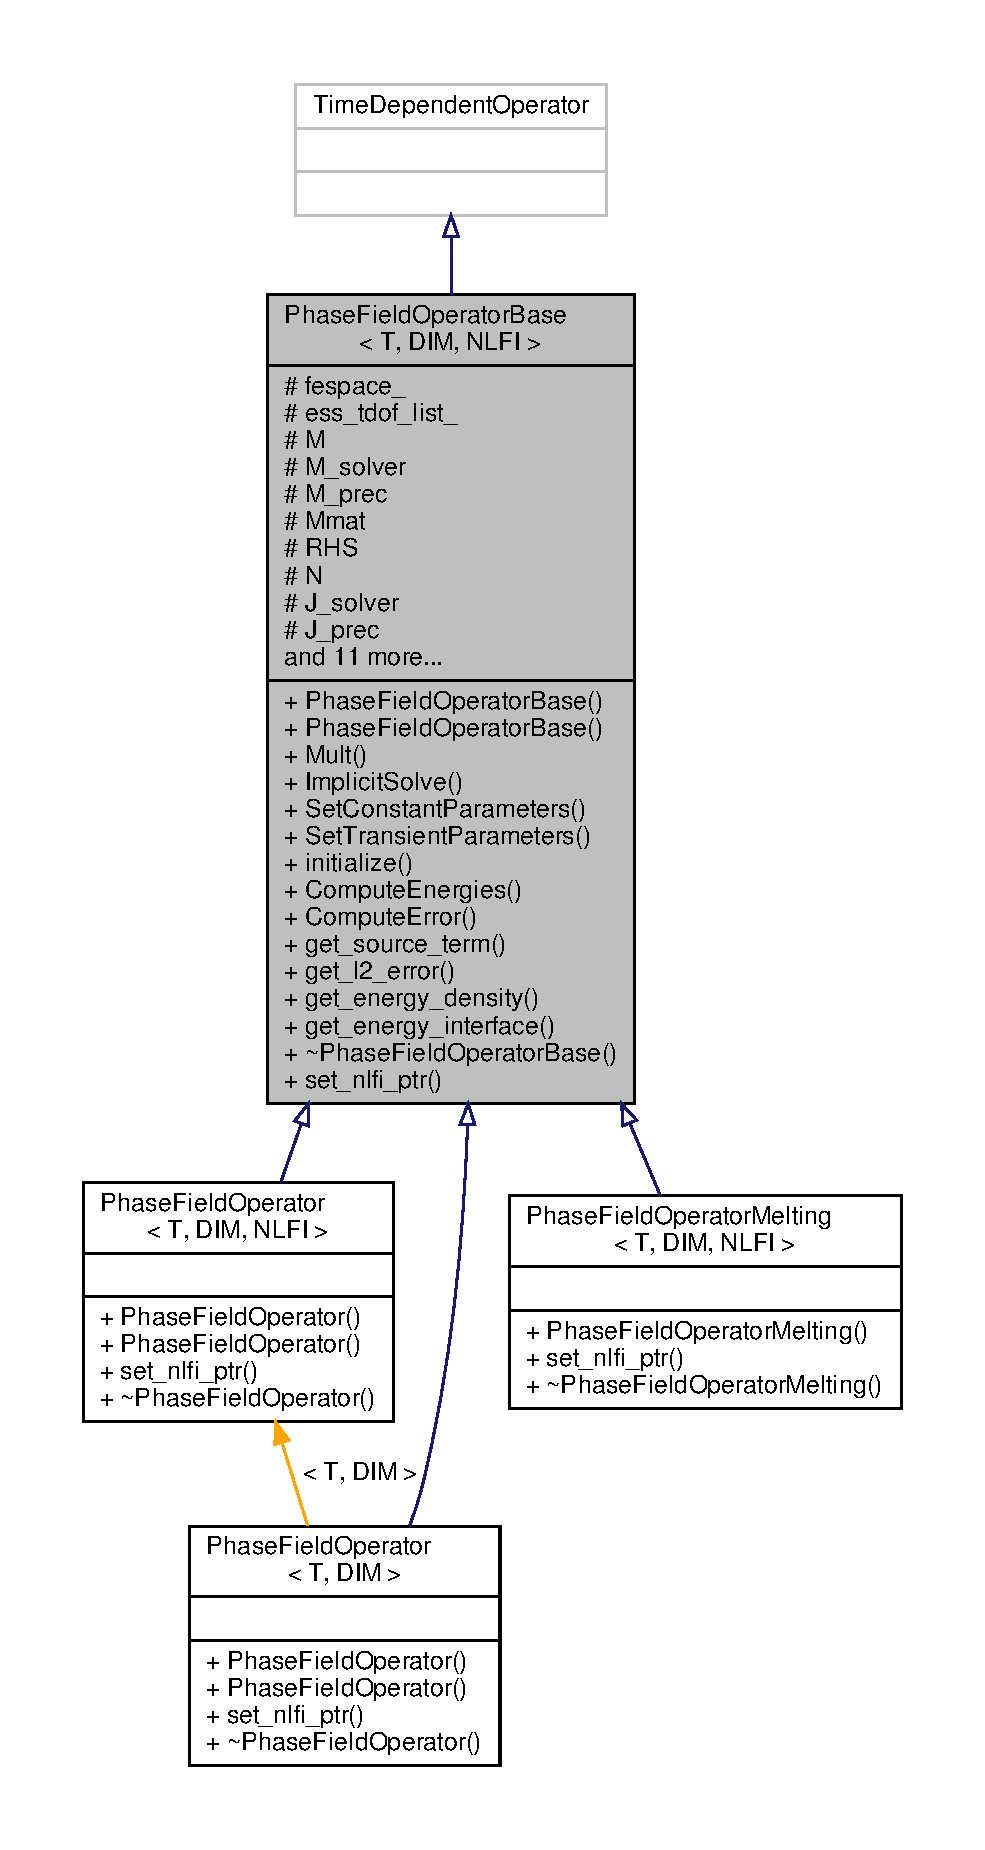
\includegraphics[height=550pt]{classPhaseFieldOperatorBase__inherit__graph}
\end{center}
\end{figure}


Collaboration diagram for Phase\+Field\+Operator\+Base$<$ T, D\+IM, N\+L\+FI $>$\+:\nopagebreak
\begin{figure}[H]
\begin{center}
\leavevmode
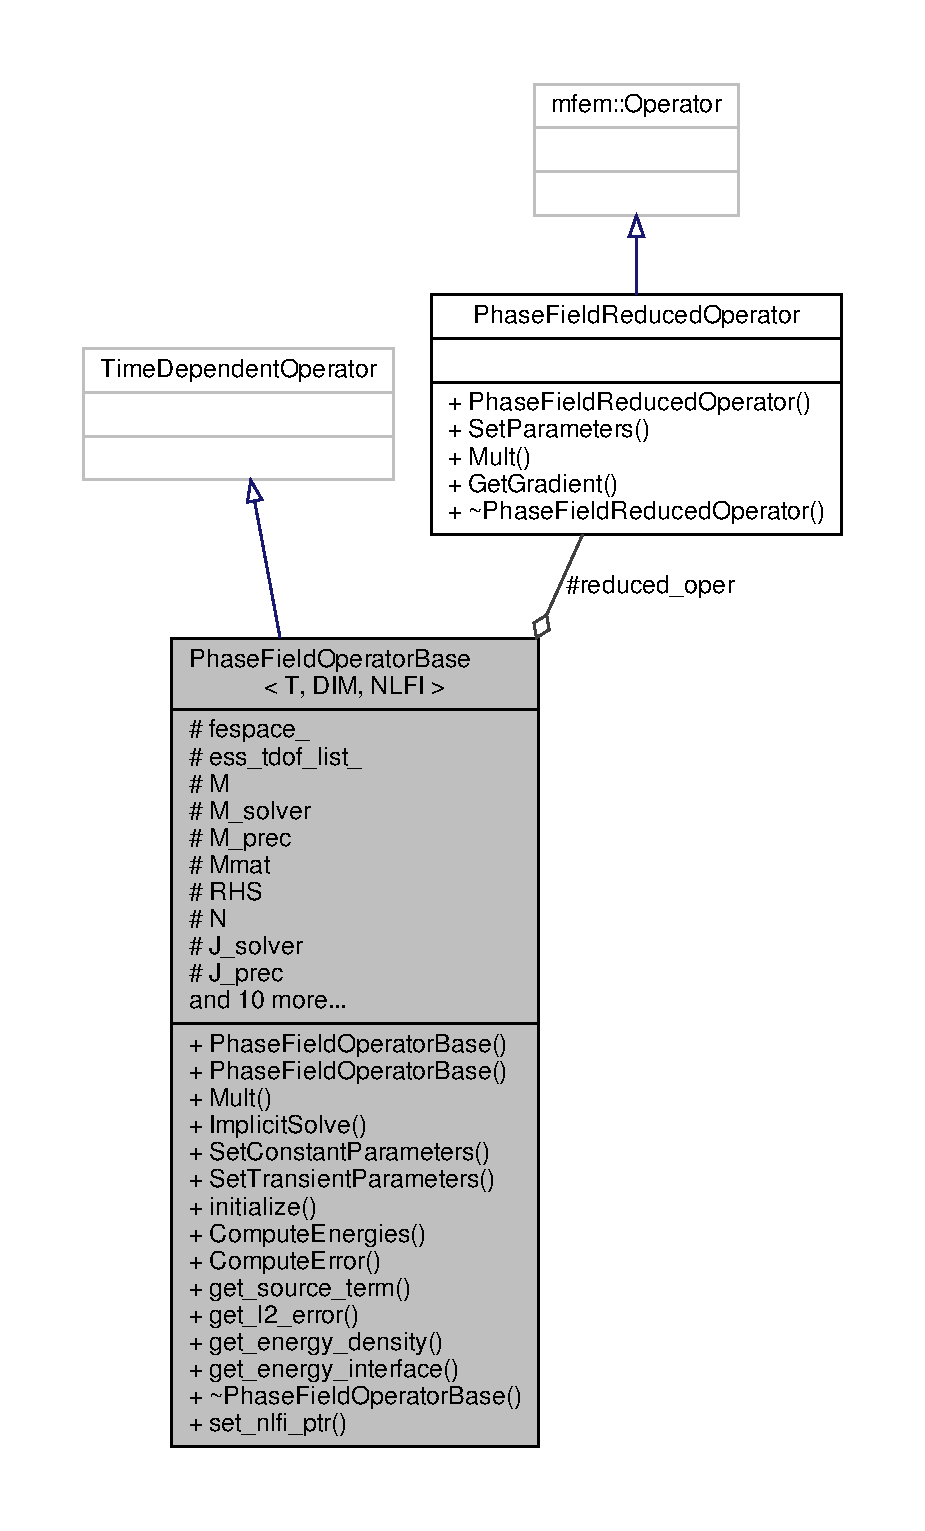
\includegraphics[height=550pt]{classPhaseFieldOperatorBase__coll__graph}
\end{center}
\end{figure}
\subsection*{Public Member Functions}
\begin{DoxyCompactItemize}
\item 
\hyperlink{classPhaseFieldOperatorBase_ae67f14dad2267b47a866e6f1dfb1f39b}{Phase\+Field\+Operator\+Base} (\hyperlink{classSpatialDiscretization}{Spatial\+Discretization}$<$ T, D\+IM $>$ $\ast$spatial, const \hyperlink{classParameters}{Parameters} \&params, \hyperlink{classVariables}{Variables}$<$ T, D\+IM $>$ \&vars)
\begin{DoxyCompactList}\small\item\em Construct a new Phase Field Operator\+:\+: Phase Field Operator object. \end{DoxyCompactList}\item 
{\footnotesize template$<$typename... Args$>$ }\\\hyperlink{classPhaseFieldOperatorBase_ae5590fe61c4339f3c22ccf7f40868500}{Phase\+Field\+Operator\+Base} (\hyperlink{classSpatialDiscretization}{Spatial\+Discretization}$<$ T, D\+IM $>$ $\ast$spatial, const \hyperlink{classParameters}{Parameters} \&params, \hyperlink{classVariables}{Variables}$<$ T, D\+IM $>$ \&vars, const std\+::string \&source\+\_\+term\+\_\+name, Args... args)
\begin{DoxyCompactList}\small\item\em Construct a new Phase Field Operator\+:\+: Phase Field Operator object. \end{DoxyCompactList}\item 
virtual void \hyperlink{classPhaseFieldOperatorBase_a55a314426a0d9bbb181cb5d35e8f76e9}{Mult} (const mfem\+::\+Vector \&u, mfem\+::\+Vector \&du\+\_\+dt) const
\begin{DoxyCompactList}\small\item\em Compute the right-\/hand side of the O\+DE system. \end{DoxyCompactList}\item 
virtual void \hyperlink{classPhaseFieldOperatorBase_ac1be84d201e35ba329090cdda6a4bfc5}{Implicit\+Solve} (const double dt, const mfem\+::\+Vector \&u, mfem\+::\+Vector \&k)
\begin{DoxyCompactList}\small\item\em Solve the Backward-\/\+Euler equation\+: k = f(phi + dt$\ast$k, t), for the unknown k. \end{DoxyCompactList}\item 
void \hyperlink{classPhaseFieldOperatorBase_ae28add1cf3731d10726a9665862a725b}{Set\+Constant\+Parameters} (const double dt, mfem\+::\+Vector \&u)
\begin{DoxyCompactList}\small\item\em Set current dt, unk values -\/ needed to compute action and Jacobian. \end{DoxyCompactList}\item 
void \hyperlink{classPhaseFieldOperatorBase_a07fb8bcd8791bb712681379c160c1ad6}{Set\+Transient\+Parameters} (const double dt, const mfem\+::\+Vector \&u)
\begin{DoxyCompactList}\small\item\em Set current dt, unk values -\/ needed to compute action and Jacobian. solution\+\_\+coef. \end{DoxyCompactList}\item 
void \hyperlink{classPhaseFieldOperatorBase_a4a85f7d2ece328d8fdb8895a2b76bd0a}{initialize} (const double \&initial\+\_\+time)
\begin{DoxyCompactList}\small\item\em Initialization stage. \end{DoxyCompactList}\item 
void \hyperlink{classPhaseFieldOperatorBase_ac313363a74691d6b500191ff475b57fb}{Compute\+Energies} (const std\+::tuple$<$ int, double, double $>$ \&iter, const mfem\+::\+Vector \&u)
\begin{DoxyCompactList}\small\item\em Compute Phase-\/field Energies. \end{DoxyCompactList}\item 
void \hyperlink{classPhaseFieldOperatorBase_ae2166b96b4d740e05c5dd1ca36e9fc8c}{Compute\+Error} (const std\+::tuple$<$ int, double, double $>$ \&iter, const mfem\+::\+Vector \&u, std\+::function$<$ double(const mfem\+::\+Vector \&, double)$>$ solution\+\_\+func)
\begin{DoxyCompactList}\small\item\em Compute L2 error. \end{DoxyCompactList}\item 
void \hyperlink{classPhaseFieldOperatorBase_ade4aaf43e627fdc8b2a3690839e225d3}{get\+\_\+source\+\_\+term} (mfem\+::\+Vector \&source\+\_\+term) const
\begin{DoxyCompactList}\small\item\em get the source term \end{DoxyCompactList}\item 
const std\+::map$<$ std\+::tuple$<$ int, double, double $>$, double $>$ \hyperlink{classPhaseFieldOperatorBase_adc993d94274e82bc06f9555fbecbd310}{get\+\_\+l2\+\_\+error} () const
\begin{DoxyCompactList}\small\item\em Get a value of a map of L2 errors at a given iteration. \end{DoxyCompactList}\item 
const std\+::map$<$ std\+::tuple$<$ int, double, double $>$, double $>$ \hyperlink{classPhaseFieldOperatorBase_a8428da5d747f60f7ccbd79c879ca8d25}{get\+\_\+energy\+\_\+density} () const
\begin{DoxyCompactList}\small\item\em Get a of a map of interfacial energy at a given iteration. \end{DoxyCompactList}\item 
const std\+::map$<$ std\+::tuple$<$ int, double, double $>$, double $>$ \hyperlink{classPhaseFieldOperatorBase_ac194823660f85a12d8edcf4520bbc025}{get\+\_\+energy\+\_\+interface} () const
\begin{DoxyCompactList}\small\item\em Get a of a map of interfacial energy at a given iteration. \end{DoxyCompactList}\item 
\mbox{\Hypertarget{classPhaseFieldOperatorBase_a2fa886ac479aa0a808a4adf57ad294ec}\label{classPhaseFieldOperatorBase_a2fa886ac479aa0a808a4adf57ad294ec}} 
virtual \hyperlink{classPhaseFieldOperatorBase_a2fa886ac479aa0a808a4adf57ad294ec}{$\sim$\+Phase\+Field\+Operator\+Base} ()
\begin{DoxyCompactList}\small\item\em Destroy the Phase Field Operator\+:\+: Phase Field Operator object. \end{DoxyCompactList}\item 
\mbox{\Hypertarget{classPhaseFieldOperatorBase_a6defeb100c4fecbd35b8591533191bc7}\label{classPhaseFieldOperatorBase_a6defeb100c4fecbd35b8591533191bc7}} 
virtual N\+L\+FI $\ast$ {\bfseries set\+\_\+nlfi\+\_\+ptr} (const double dt, const mfem\+::\+Vector \&u)=0
\end{DoxyCompactItemize}
\subsection*{Protected Attributes}
\begin{DoxyCompactItemize}
\item 
\mbox{\Hypertarget{classPhaseFieldOperatorBase_ac8697ec5f9f8b2098f695403b7e7d32c}\label{classPhaseFieldOperatorBase_ac8697ec5f9f8b2098f695403b7e7d32c}} 
mfem\+::\+Finite\+Element\+Space $\ast$ {\bfseries fespace\+\_\+}
\item 
\mbox{\Hypertarget{classPhaseFieldOperatorBase_aef9d79b193e695484fc8ece8280a3c6e}\label{classPhaseFieldOperatorBase_aef9d79b193e695484fc8ece8280a3c6e}} 
mfem\+::\+Array$<$ int $>$ {\bfseries ess\+\_\+tdof\+\_\+list\+\_\+}
\item 
\mbox{\Hypertarget{classPhaseFieldOperatorBase_ac59727af25abdd5a0b0eff6a7e766ed2}\label{classPhaseFieldOperatorBase_ac59727af25abdd5a0b0eff6a7e766ed2}} 
mfem\+::\+Bilinear\+Form $\ast$ {\bfseries M}
\item 
\mbox{\Hypertarget{classPhaseFieldOperatorBase_abae6aa970af1afee541f399716c84459}\label{classPhaseFieldOperatorBase_abae6aa970af1afee541f399716c84459}} 
mfem\+::\+C\+G\+Solver {\bfseries M\+\_\+solver}
\item 
\mbox{\Hypertarget{classPhaseFieldOperatorBase_ae0ff8b7ef560d3bde9b6ba13585f57bd}\label{classPhaseFieldOperatorBase_ae0ff8b7ef560d3bde9b6ba13585f57bd}} 
mfem\+::\+D\+Smoother {\bfseries M\+\_\+prec}
\item 
\mbox{\Hypertarget{classPhaseFieldOperatorBase_a3623bbe799103af42de43d798bb3e928}\label{classPhaseFieldOperatorBase_a3623bbe799103af42de43d798bb3e928}} 
mfem\+::\+Sparse\+Matrix {\bfseries Mmat}
\item 
\mbox{\Hypertarget{classPhaseFieldOperatorBase_ab4ba4f88819f656ce8f6dddee6ded24f}\label{classPhaseFieldOperatorBase_ab4ba4f88819f656ce8f6dddee6ded24f}} 
mfem\+::\+Linear\+Form $\ast$ {\bfseries R\+HS}
\item 
\mbox{\Hypertarget{classPhaseFieldOperatorBase_a235f1d2f65754932ca9f1fbfd7f91d91}\label{classPhaseFieldOperatorBase_a235f1d2f65754932ca9f1fbfd7f91d91}} 
mfem\+::\+Nonlinear\+Form $\ast$ {\bfseries N}
\item 
\mbox{\Hypertarget{classPhaseFieldOperatorBase_af0cc6c282ae76674384e3d6a87aa88d9}\label{classPhaseFieldOperatorBase_af0cc6c282ae76674384e3d6a87aa88d9}} 
mfem\+::\+Solver $\ast$ {\bfseries J\+\_\+solver}
\item 
\mbox{\Hypertarget{classPhaseFieldOperatorBase_ab907d8e1cbd9d399959064f8fed3c3e6}\label{classPhaseFieldOperatorBase_ab907d8e1cbd9d399959064f8fed3c3e6}} 
mfem\+::\+Solver $\ast$ {\bfseries J\+\_\+prec}
\item 
\mbox{\Hypertarget{classPhaseFieldOperatorBase_ace8edd3371a4b1b1adaf22a36ad2041a}\label{classPhaseFieldOperatorBase_ace8edd3371a4b1b1adaf22a36ad2041a}} 
\hyperlink{classBoundaryConditions}{Boundary\+Conditions}$<$ T, D\+IM $>$ $\ast$ {\bfseries bcs\+\_\+}
\item 
\mbox{\Hypertarget{classPhaseFieldOperatorBase_a7613689c7c934e661ec287b7b878c9d2}\label{classPhaseFieldOperatorBase_a7613689c7c934e661ec287b7b878c9d2}} 
\hyperlink{classVariables}{Variables}$<$ T, D\+IM $>$ {\bfseries vars\+\_\+}
\item 
\mbox{\Hypertarget{classPhaseFieldOperatorBase_ae643a34ec21563a1aa1e0baee30beb30}\label{classPhaseFieldOperatorBase_ae643a34ec21563a1aa1e0baee30beb30}} 
mfem\+::\+Newton\+Solver {\bfseries newton\+\_\+solver\+\_\+}
\item 
\hyperlink{classPhaseFieldReducedOperator}{Phase\+Field\+Reduced\+Operator} $\ast$ \hyperlink{classPhaseFieldOperatorBase_a010a3da035afe945635288cc0ab2f0b5}{reduced\+\_\+oper}
\item 
\mbox{\Hypertarget{classPhaseFieldOperatorBase_aaa799d0dbf5d04e158f276cc3e0a32cc}\label{classPhaseFieldOperatorBase_aaa799d0dbf5d04e158f276cc3e0a32cc}} 
double {\bfseries mobility\+\_\+coeff\+\_\+}
\item 
\mbox{\Hypertarget{classPhaseFieldOperatorBase_a275f0cce177c9cd3c2cced2771b8f702}\label{classPhaseFieldOperatorBase_a275f0cce177c9cd3c2cced2771b8f702}} 
double {\bfseries omega\+\_\+}
\item 
\mbox{\Hypertarget{classPhaseFieldOperatorBase_a55ca706b0f6f4ee16eb1c27523569a2c}\label{classPhaseFieldOperatorBase_a55ca706b0f6f4ee16eb1c27523569a2c}} 
double {\bfseries lambda\+\_\+}
\item 
\mbox{\Hypertarget{classPhaseFieldOperatorBase_a1cc7b7915970f927c7e3bde1d06b9412}\label{classPhaseFieldOperatorBase_a1cc7b7915970f927c7e3bde1d06b9412}} 
std\+::function$<$ double(const mfem\+::\+Vector \&, double)$>$ {\bfseries src\+\_\+func\+\_\+}
\item 
\mbox{\Hypertarget{classPhaseFieldOperatorBase_ac7c9e3138a6324901705e74da62421ea}\label{classPhaseFieldOperatorBase_ac7c9e3138a6324901705e74da62421ea}} 
double {\bfseries current\+\_\+dt\+\_\+}
\item 
\mbox{\Hypertarget{classPhaseFieldOperatorBase_a67fca8849db8e5659f633a2c0df694b7}\label{classPhaseFieldOperatorBase_a67fca8849db8e5659f633a2c0df694b7}} 
mfem\+::\+Vector {\bfseries z}
\item 
\mbox{\Hypertarget{classPhaseFieldOperatorBase_aefbc006a9f535e2ab69a9a8964e2b159}\label{classPhaseFieldOperatorBase_aefbc006a9f535e2ab69a9a8964e2b159}} 
std\+::string {\bfseries source\+\_\+term\+\_\+name\+\_\+}
\end{DoxyCompactItemize}


\subsection{Detailed Description}
\subsubsection*{template$<$class T, int D\+IM, class N\+L\+FI$>$\newline
class Phase\+Field\+Operator\+Base$<$ T, D\+I\+M, N\+L\+F\+I $>$}

\hyperlink{classPhaseFieldOperatorBase}{Phase\+Field\+Operator\+Base} class. 

Definition at line 48 of file Phase\+Field\+Operator\+Base.\+hpp.



\subsection{Constructor \& Destructor Documentation}
\mbox{\Hypertarget{classPhaseFieldOperatorBase_ae67f14dad2267b47a866e6f1dfb1f39b}\label{classPhaseFieldOperatorBase_ae67f14dad2267b47a866e6f1dfb1f39b}} 
\index{Phase\+Field\+Operator\+Base@{Phase\+Field\+Operator\+Base}!Phase\+Field\+Operator\+Base@{Phase\+Field\+Operator\+Base}}
\index{Phase\+Field\+Operator\+Base@{Phase\+Field\+Operator\+Base}!Phase\+Field\+Operator\+Base@{Phase\+Field\+Operator\+Base}}
\subsubsection{\texorpdfstring{Phase\+Field\+Operator\+Base()}{PhaseFieldOperatorBase()}\hspace{0.1cm}{\footnotesize\ttfamily [1/2]}}
{\footnotesize\ttfamily template$<$class T , int D\+IM, class N\+L\+FI $>$ \\
\hyperlink{classPhaseFieldOperatorBase}{Phase\+Field\+Operator\+Base}$<$ T, D\+IM, N\+L\+FI $>$\+::\hyperlink{classPhaseFieldOperatorBase}{Phase\+Field\+Operator\+Base} (\begin{DoxyParamCaption}\item[{\hyperlink{classSpatialDiscretization}{Spatial\+Discretization}$<$ T, D\+IM $>$ $\ast$}]{spatial,  }\item[{const \hyperlink{classParameters}{Parameters} \&}]{params,  }\item[{\hyperlink{classVariables}{Variables}$<$ T, D\+IM $>$ \&}]{vars }\end{DoxyParamCaption})}



Construct a new Phase Field Operator\+:\+: Phase Field Operator object. 


\begin{DoxyParams}{Parameters}
{\em fespace} & Finite Element space \\
\hline
{\em params} & list of \hyperlink{classParameters}{Parameters} \\
\hline
{\em u} & unknown vector \\
\hline
\end{DoxyParams}


Definition at line 132 of file Phase\+Field\+Operator\+Base.\+hpp.



References Spatial\+Discretization$<$ T, D\+I\+M $>$\+::get\+\_\+finite\+\_\+element\+\_\+space(), and Parameters\+::get\+\_\+parameter\+\_\+value().


\begin{DoxyCode}
135     : mfem::TimeDependentOperator(spatial->\hyperlink{classSpatialDiscretization_a2f23ae965741d678ef45c6a545ce9a9d}{getSize}(), 0.0),
136       M(NULL),
137       N(NULL),
138       vars\_(vars),
139       current\_dt\_(0.0),
140       z(height) \{
141   this->fespace\_ = spatial->\hyperlink{classSpatialDiscretization_ac001fc2ff356fe8c0c2b49618e594a03}{get\_finite\_element\_space}();
142   this->omega\_ = params.\hyperlink{classParameters_ab1bac6bf07b9698c850542b68e143ef3}{get\_parameter\_value}(\textcolor{stringliteral}{"omega"});
143   this->lambda\_ = params.\hyperlink{classParameters_ab1bac6bf07b9698c850542b68e143ef3}{get\_parameter\_value}(\textcolor{stringliteral}{"lambda"});
144   this->mobility\_coeff\_ = params.\hyperlink{classParameters_ab1bac6bf07b9698c850542b68e143ef3}{get\_parameter\_value}(\textcolor{stringliteral}{"mobility"});
145 \}
\end{DoxyCode}
\mbox{\Hypertarget{classPhaseFieldOperatorBase_ae5590fe61c4339f3c22ccf7f40868500}\label{classPhaseFieldOperatorBase_ae5590fe61c4339f3c22ccf7f40868500}} 
\index{Phase\+Field\+Operator\+Base@{Phase\+Field\+Operator\+Base}!Phase\+Field\+Operator\+Base@{Phase\+Field\+Operator\+Base}}
\index{Phase\+Field\+Operator\+Base@{Phase\+Field\+Operator\+Base}!Phase\+Field\+Operator\+Base@{Phase\+Field\+Operator\+Base}}
\subsubsection{\texorpdfstring{Phase\+Field\+Operator\+Base()}{PhaseFieldOperatorBase()}\hspace{0.1cm}{\footnotesize\ttfamily [2/2]}}
{\footnotesize\ttfamily template$<$class T , int D\+IM, class N\+L\+FI $>$ \\
template$<$typename... Args$>$ \\
\hyperlink{classPhaseFieldOperatorBase}{Phase\+Field\+Operator\+Base}$<$ T, D\+IM, N\+L\+FI $>$\+::\hyperlink{classPhaseFieldOperatorBase}{Phase\+Field\+Operator\+Base} (\begin{DoxyParamCaption}\item[{\hyperlink{classSpatialDiscretization}{Spatial\+Discretization}$<$ T, D\+IM $>$ $\ast$}]{spatial,  }\item[{const \hyperlink{classParameters}{Parameters} \&}]{params,  }\item[{\hyperlink{classVariables}{Variables}$<$ T, D\+IM $>$ \&}]{vars,  }\item[{const std\+::string \&}]{source\+\_\+term\+\_\+name,  }\item[{Args...}]{args }\end{DoxyParamCaption})}



Construct a new Phase Field Operator\+:\+: Phase Field Operator object. 


\begin{DoxyParams}{Parameters}
{\em fespace} & Finite Element space \\
\hline
{\em params} & list of \hyperlink{classParameters}{Parameters} \\
\hline
{\em u} & unknown vector \\
\hline
\end{DoxyParams}


Definition at line 157 of file Phase\+Field\+Operator\+Base.\+hpp.



References Spatial\+Discretization$<$ T, D\+I\+M $>$\+::get\+\_\+finite\+\_\+element\+\_\+space(), Parameters\+::get\+\_\+parameter\+\_\+value(), and Analytical\+Functions$<$ D\+I\+M $>$\+::get\+Analytical\+Functions().


\begin{DoxyCode}
162     : mfem::TimeDependentOperator(spatial->\hyperlink{classSpatialDiscretization_a2f23ae965741d678ef45c6a545ce9a9d}{getSize}(), 0.0),
163       M(NULL),
164       N(NULL),
165       vars\_(vars),
166       current\_dt\_(0.0),
167       z(height),
168       source\_term\_name\_(source\_term\_name) \{
169   this->fespace\_ = spatial->\hyperlink{classSpatialDiscretization_ac001fc2ff356fe8c0c2b49618e594a03}{get\_finite\_element\_space}();
170   this->omega\_ = params.\hyperlink{classParameters_ab1bac6bf07b9698c850542b68e143ef3}{get\_parameter\_value}(\textcolor{stringliteral}{"omega"});
171   this->lambda\_ = params.\hyperlink{classParameters_ab1bac6bf07b9698c850542b68e143ef3}{get\_parameter\_value}(\textcolor{stringliteral}{"lambda"});
172   this->mobility\_coeff\_ = params.\hyperlink{classParameters_ab1bac6bf07b9698c850542b68e143ef3}{get\_parameter\_value}(\textcolor{stringliteral}{"mobility"});
173   \hyperlink{classAnalyticalFunctions}{AnalyticalFunctions<DIM>} source\_func;
174   this->src\_func\_ = source\_func.\hyperlink{classAnalyticalFunctions_a88a27c868b872e12d16f1097779fd3f8}{getAnalyticalFunctions}(this->source\_term\_name\_, args.
      ..);
175 
176   \textcolor{comment}{// auto &vv = vars.get\_variable("phi");}
177   \textcolor{comment}{// this->initialize(vv);}
178 \}
\end{DoxyCode}


\subsection{Member Function Documentation}
\mbox{\Hypertarget{classPhaseFieldOperatorBase_ac313363a74691d6b500191ff475b57fb}\label{classPhaseFieldOperatorBase_ac313363a74691d6b500191ff475b57fb}} 
\index{Phase\+Field\+Operator\+Base@{Phase\+Field\+Operator\+Base}!Compute\+Energies@{Compute\+Energies}}
\index{Compute\+Energies@{Compute\+Energies}!Phase\+Field\+Operator\+Base@{Phase\+Field\+Operator\+Base}}
\subsubsection{\texorpdfstring{Compute\+Energies()}{ComputeEnergies()}}
{\footnotesize\ttfamily template$<$class T , int D\+IM, class N\+L\+FI $>$ \\
void \hyperlink{classPhaseFieldOperatorBase}{Phase\+Field\+Operator\+Base}$<$ T, D\+IM, N\+L\+FI $>$\+::Compute\+Energies (\begin{DoxyParamCaption}\item[{const std\+::tuple$<$ int, double, double $>$ \&}]{iter,  }\item[{const mfem\+::\+Vector \&}]{u }\end{DoxyParamCaption})}



Compute Phase-\/field Energies. 


\begin{DoxyParams}{Parameters}
{\em u} & unknown vector \\
\hline
\end{DoxyParams}
\begin{DoxyReturn}{Returns}
const double 
\end{DoxyReturn}


Definition at line 338 of file Phase\+Field\+Operator\+Base.\+hpp.


\begin{DoxyCode}
339                                                                     \{
340   mfem::GridFunction un\_gf(this->fespace\_);
341   un\_gf.SetFromTrueDofs(u);
342   mfem::GridFunction gf(this->fespace\_);
343   \hyperlink{classEnergyCoefficient}{EnergyCoefficient} g(&un\_gf, 0.5 * this->lambda\_, this->omega\_);
344   gf.ProjectCoefficient(g);
345   mfem::GridFunction sigf(this->fespace\_);
346   \hyperlink{classEnergyCoefficient}{EnergyCoefficient} sig(&un\_gf, this->lambda\_, 0.);
347   sigf.ProjectCoefficient(sig);
348 
349   \textcolor{comment}{// Calcul de l'intégrale de l'objet FunctionCoefficient sur le domaine}
350   mfem::ConstantCoefficient zero(0.);
351   \textcolor{keyword}{const} \textcolor{keyword}{auto} energy = gf.ComputeL1Error(zero);
352   this->energy\_density\_.try\_emplace(iter, energy);
353   \textcolor{keyword}{const} \textcolor{keyword}{auto} interfacial\_energy = sigf.ComputeL1Error(zero);
354   this->energy\_interface\_.try\_emplace(iter, interfacial\_energy);
355 \}
\end{DoxyCode}
\mbox{\Hypertarget{classPhaseFieldOperatorBase_ae2166b96b4d740e05c5dd1ca36e9fc8c}\label{classPhaseFieldOperatorBase_ae2166b96b4d740e05c5dd1ca36e9fc8c}} 
\index{Phase\+Field\+Operator\+Base@{Phase\+Field\+Operator\+Base}!Compute\+Error@{Compute\+Error}}
\index{Compute\+Error@{Compute\+Error}!Phase\+Field\+Operator\+Base@{Phase\+Field\+Operator\+Base}}
\subsubsection{\texorpdfstring{Compute\+Error()}{ComputeError()}}
{\footnotesize\ttfamily template$<$class T , int D\+IM, class N\+L\+FI $>$ \\
void \hyperlink{classPhaseFieldOperatorBase}{Phase\+Field\+Operator\+Base}$<$ T, D\+IM, N\+L\+FI $>$\+::Compute\+Error (\begin{DoxyParamCaption}\item[{const std\+::tuple$<$ int, double, double $>$ \&}]{iter,  }\item[{const mfem\+::\+Vector \&}]{u,  }\item[{std\+::function$<$ double(const mfem\+::\+Vector \&, double)$>$}]{solution\+\_\+func }\end{DoxyParamCaption})}



Compute L2 error. 


\begin{DoxyParams}{Parameters}
{\em u} & unknown vector \\
\hline
\end{DoxyParams}
\begin{DoxyReturn}{Returns}
const double 
\end{DoxyReturn}


Definition at line 364 of file Phase\+Field\+Operator\+Base.\+hpp.


\begin{DoxyCode}
366                                                                    \{
367   mfem::GridFunction gf(this->fespace\_);
368   gf.SetFromTrueDofs(u);
369   mfem::FunctionCoefficient solution\_coef(solution\_func);
370   solution\_coef.SetTime(this->GetTime());
371   \textcolor{keyword}{const} \textcolor{keyword}{auto} error = gf.ComputeL2Error(solution\_coef);
372   this->error\_l2\_.try\_emplace(iter, error);
373 \}
\end{DoxyCode}
\mbox{\Hypertarget{classPhaseFieldOperatorBase_a8428da5d747f60f7ccbd79c879ca8d25}\label{classPhaseFieldOperatorBase_a8428da5d747f60f7ccbd79c879ca8d25}} 
\index{Phase\+Field\+Operator\+Base@{Phase\+Field\+Operator\+Base}!get\+\_\+energy\+\_\+density@{get\+\_\+energy\+\_\+density}}
\index{get\+\_\+energy\+\_\+density@{get\+\_\+energy\+\_\+density}!Phase\+Field\+Operator\+Base@{Phase\+Field\+Operator\+Base}}
\subsubsection{\texorpdfstring{get\+\_\+energy\+\_\+density()}{get\_energy\_density()}}
{\footnotesize\ttfamily template$<$class T , int D\+IM, class N\+L\+FI $>$ \\
const std\+::map$<$ std\+::tuple$<$ int, double, double $>$, double $>$ \hyperlink{classPhaseFieldOperatorBase}{Phase\+Field\+Operator\+Base}$<$ T, D\+IM, N\+L\+FI $>$\+::get\+\_\+energy\+\_\+density (\begin{DoxyParamCaption}{ }\end{DoxyParamCaption}) const}



Get a of a map of interfacial energy at a given iteration. 


\begin{DoxyTemplParams}{Template Parameters}
{\em T} & \\
\hline
{\em D\+IM} & \\
\hline
{\em N\+L\+FI} & \\
\hline
\end{DoxyTemplParams}
\begin{DoxyReturn}{Returns}
const std\+::map$<$std\+::tuple$<$int, double, double$>$, double$>$ 
\end{DoxyReturn}


Definition at line 417 of file Phase\+Field\+Operator\+Base.\+hpp.


\begin{DoxyCode}
417                                                                \{
418   \textcolor{keywordflow}{return} this->energy\_density\_;
419 \}
\end{DoxyCode}
\mbox{\Hypertarget{classPhaseFieldOperatorBase_ac194823660f85a12d8edcf4520bbc025}\label{classPhaseFieldOperatorBase_ac194823660f85a12d8edcf4520bbc025}} 
\index{Phase\+Field\+Operator\+Base@{Phase\+Field\+Operator\+Base}!get\+\_\+energy\+\_\+interface@{get\+\_\+energy\+\_\+interface}}
\index{get\+\_\+energy\+\_\+interface@{get\+\_\+energy\+\_\+interface}!Phase\+Field\+Operator\+Base@{Phase\+Field\+Operator\+Base}}
\subsubsection{\texorpdfstring{get\+\_\+energy\+\_\+interface()}{get\_energy\_interface()}}
{\footnotesize\ttfamily template$<$class T , int D\+IM, class N\+L\+FI $>$ \\
const std\+::map$<$ std\+::tuple$<$ int, double, double $>$, double $>$ \hyperlink{classPhaseFieldOperatorBase}{Phase\+Field\+Operator\+Base}$<$ T, D\+IM, N\+L\+FI $>$\+::get\+\_\+energy\+\_\+interface (\begin{DoxyParamCaption}{ }\end{DoxyParamCaption}) const}



Get a of a map of interfacial energy at a given iteration. 


\begin{DoxyTemplParams}{Template Parameters}
{\em T} & \\
\hline
{\em D\+IM} & \\
\hline
{\em N\+L\+FI} & \\
\hline
\end{DoxyTemplParams}
\begin{DoxyReturn}{Returns}
const std\+::map$<$std\+::tuple$<$int, double, double$>$, double$>$ 
\end{DoxyReturn}


Definition at line 431 of file Phase\+Field\+Operator\+Base.\+hpp.


\begin{DoxyCode}
431                                                                  \{
432   \textcolor{keywordflow}{return} this->energy\_interface\_;
433 \}
\end{DoxyCode}
\mbox{\Hypertarget{classPhaseFieldOperatorBase_adc993d94274e82bc06f9555fbecbd310}\label{classPhaseFieldOperatorBase_adc993d94274e82bc06f9555fbecbd310}} 
\index{Phase\+Field\+Operator\+Base@{Phase\+Field\+Operator\+Base}!get\+\_\+l2\+\_\+error@{get\+\_\+l2\+\_\+error}}
\index{get\+\_\+l2\+\_\+error@{get\+\_\+l2\+\_\+error}!Phase\+Field\+Operator\+Base@{Phase\+Field\+Operator\+Base}}
\subsubsection{\texorpdfstring{get\+\_\+l2\+\_\+error()}{get\_l2\_error()}}
{\footnotesize\ttfamily template$<$class T , int D\+IM, class N\+L\+FI $>$ \\
const std\+::map$<$ std\+::tuple$<$ int, double, double $>$, double $>$ \hyperlink{classPhaseFieldOperatorBase}{Phase\+Field\+Operator\+Base}$<$ T, D\+IM, N\+L\+FI $>$\+::get\+\_\+l2\+\_\+error (\begin{DoxyParamCaption}{ }\end{DoxyParamCaption}) const}



Get a value of a map of L2 errors at a given iteration. 


\begin{DoxyTemplParams}{Template Parameters}
{\em T} & \\
\hline
{\em D\+IM} & \\
\hline
{\em N\+L\+FI} & \\
\hline
\end{DoxyTemplParams}

\begin{DoxyParams}{Parameters}
{\em iter} & \\
\hline
\end{DoxyParams}
\begin{DoxyReturn}{Returns}
const std\+::map$<$std\+::tuple$<$int, double, double$>$, double$>$ 
\end{DoxyReturn}


Definition at line 403 of file Phase\+Field\+Operator\+Base.\+hpp.


\begin{DoxyCode}
403                                                          \{
404   \textcolor{keywordflow}{return} this->error\_l2\_;
405 \}
\end{DoxyCode}
\mbox{\Hypertarget{classPhaseFieldOperatorBase_ade4aaf43e627fdc8b2a3690839e225d3}\label{classPhaseFieldOperatorBase_ade4aaf43e627fdc8b2a3690839e225d3}} 
\index{Phase\+Field\+Operator\+Base@{Phase\+Field\+Operator\+Base}!get\+\_\+source\+\_\+term@{get\+\_\+source\+\_\+term}}
\index{get\+\_\+source\+\_\+term@{get\+\_\+source\+\_\+term}!Phase\+Field\+Operator\+Base@{Phase\+Field\+Operator\+Base}}
\subsubsection{\texorpdfstring{get\+\_\+source\+\_\+term()}{get\_source\_term()}}
{\footnotesize\ttfamily template$<$class T , int D\+IM, class N\+L\+FI $>$ \\
void \hyperlink{classPhaseFieldOperatorBase}{Phase\+Field\+Operator\+Base}$<$ T, D\+IM, N\+L\+FI $>$\+::get\+\_\+source\+\_\+term (\begin{DoxyParamCaption}\item[{mfem\+::\+Vector \&}]{source\+\_\+term }\end{DoxyParamCaption}) const}



get the source term 


\begin{DoxyTemplParams}{Template Parameters}
{\em T} & \\
\hline
{\em D\+IM} & \\
\hline
{\em N\+L\+FI} & \\
\hline
\end{DoxyTemplParams}


Definition at line 383 of file Phase\+Field\+Operator\+Base.\+hpp.



Referenced by Phase\+Field\+Operator\+Base$<$ T, D\+I\+M, N\+L\+F\+I $>$\+::\+Implicit\+Solve(), and Phase\+Field\+Operator\+Base$<$ T, D\+I\+M, N\+L\+F\+I $>$\+::\+Mult().


\begin{DoxyCode}
383                                                                                         \{
384   std::shared\_ptr<mfem::LinearForm> RHSS(\textcolor{keyword}{new} mfem::LinearForm(this->fespace\_));
385   mfem::FunctionCoefficient src(this->src\_func\_);
386   src.SetTime(this->GetTime());
387   RHSS->AddDomainIntegrator(\textcolor{keyword}{new} mfem::DomainLFIntegrator(src));
388   RHSS->Assemble();
389   source\_term = *RHSS.get();
390 \}
\end{DoxyCode}
\mbox{\Hypertarget{classPhaseFieldOperatorBase_ac1be84d201e35ba329090cdda6a4bfc5}\label{classPhaseFieldOperatorBase_ac1be84d201e35ba329090cdda6a4bfc5}} 
\index{Phase\+Field\+Operator\+Base@{Phase\+Field\+Operator\+Base}!Implicit\+Solve@{Implicit\+Solve}}
\index{Implicit\+Solve@{Implicit\+Solve}!Phase\+Field\+Operator\+Base@{Phase\+Field\+Operator\+Base}}
\subsubsection{\texorpdfstring{Implicit\+Solve()}{ImplicitSolve()}}
{\footnotesize\ttfamily template$<$class T , int D\+IM, class N\+L\+FI $>$ \\
void \hyperlink{classPhaseFieldOperatorBase}{Phase\+Field\+Operator\+Base}$<$ T, D\+IM, N\+L\+FI $>$\+::Implicit\+Solve (\begin{DoxyParamCaption}\item[{const double}]{dt,  }\item[{const mfem\+::\+Vector \&}]{u,  }\item[{mfem\+::\+Vector \&}]{du\+\_\+dt }\end{DoxyParamCaption})\hspace{0.3cm}{\ttfamily [virtual]}}



Solve the Backward-\/\+Euler equation\+: k = f(phi + dt$\ast$k, t), for the unknown k. 

Solve the Backward-\/\+Euler equation\+: k = f(u + dt$\ast$k, t), for the unknown k. This is the only requirement for high-\/order S\+D\+I\+RK implicit integration.


\begin{DoxyParams}{Parameters}
{\em dt} & current time step \\
\hline
{\em u} & unknown vector \\
\hline
{\em du\+\_\+dt} & unkwon time derivative vector \\
\hline
\end{DoxyParams}


Definition at line 302 of file Phase\+Field\+Operator\+Base.\+hpp.



References Phase\+Field\+Operator\+Base$<$ T, D\+I\+M, N\+L\+F\+I $>$\+::get\+\_\+source\+\_\+term(), Boundary\+Conditions$<$ T, D\+I\+M $>$\+::\+Set\+Boundary\+Conditions(), Phase\+Field\+Reduced\+Operator\+::\+Set\+Parameters(), and Phase\+Field\+Operator\+Base$<$ T, D\+I\+M, N\+L\+F\+I $>$\+::\+Set\+Transient\+Parameters().


\begin{DoxyCode}
303                                                                             \{
304   \textcolor{keyword}{const} \textcolor{keyword}{auto} sc = height;
305   mfem::Vector v(u.GetData(), sc);
306   mfem::Vector dv\_dt(du\_dt.GetData(), sc);
307   \textcolor{comment}{// // Solve the equation:}
308   \textcolor{comment}{// //    du\_dt = M^\{-1\}*[-K(u + dt*du\_dt)]}
309   \textcolor{comment}{// // for du\_dt}
310 
311   this->bcs\_->SetBoundaryConditions(v);
312   this->\hyperlink{classPhaseFieldOperatorBase_a07fb8bcd8791bb712681379c160c1ad6}{SetTransientParameters}(dt, v);
313 
314   \hyperlink{classPhaseFieldOperatorBase_a010a3da035afe945635288cc0ab2f0b5}{reduced\_oper}->\hyperlink{classPhaseFieldReducedOperator_aaaa55d33260a9dc98051bd97f916bf46}{SetParameters}(dt, &v);
315 
316   \textcolor{comment}{// Source term}
317   mfem::Vector source\_term;
318   \textcolor{keywordflow}{if} (!this->source\_term\_name\_.empty()) \{
319     this->\hyperlink{classPhaseFieldOperatorBase_ade4aaf43e627fdc8b2a3690839e225d3}{get\_source\_term}(source\_term);
320   \}
321 
322   dv\_dt = v;
323   dv\_dt *= (1. / dt);
324   this->newton\_solver\_.Mult(source\_term, dv\_dt);
325   dv\_dt.SetSubVector(this->ess\_tdof\_list\_, 0.0);  \textcolor{comment}{// pour  Dirichlet ... uniquement?}
326   \textcolor{comment}{// std::cout << " PhaseFieldOperatorBase this->newton\_solver\_->Mult " << std::endl;}
327 
328   MFEM\_VERIFY(this->newton\_solver\_.GetConverged(), \textcolor{stringliteral}{"Nonlinear solver did not converge."});
329 \}
\end{DoxyCode}
\mbox{\Hypertarget{classPhaseFieldOperatorBase_a4a85f7d2ece328d8fdb8895a2b76bd0a}\label{classPhaseFieldOperatorBase_a4a85f7d2ece328d8fdb8895a2b76bd0a}} 
\index{Phase\+Field\+Operator\+Base@{Phase\+Field\+Operator\+Base}!initialize@{initialize}}
\index{initialize@{initialize}!Phase\+Field\+Operator\+Base@{Phase\+Field\+Operator\+Base}}
\subsubsection{\texorpdfstring{initialize()}{initialize()}}
{\footnotesize\ttfamily template$<$class T , int D\+IM, class N\+L\+FI $>$ \\
void \hyperlink{classPhaseFieldOperatorBase}{Phase\+Field\+Operator\+Base}$<$ T, D\+IM, N\+L\+FI $>$\+::initialize (\begin{DoxyParamCaption}\item[{const double \&}]{initial\+\_\+time }\end{DoxyParamCaption})}



Initialization stage. 


\begin{DoxyParams}{Parameters}
{\em vv} & \\
\hline
\end{DoxyParams}


Definition at line 186 of file Phase\+Field\+Operator\+Base.\+hpp.



References Variables$<$ T, D\+I\+M $>$\+::get\+\_\+variable(), Boundary\+Conditions$<$ T, D\+I\+M $>$\+::\+Get\+Essential\+Dofs(), Boundary\+Conditions$<$ T, D\+I\+M $>$\+::\+Set\+Boundary\+Conditions(), Phase\+Field\+Operator\+Base$<$ T, D\+I\+M, N\+L\+F\+I $>$\+::\+Set\+Constant\+Parameters(), and Phase\+Field\+Operator\+Base$<$ T, D\+I\+M, N\+L\+F\+I $>$\+::\+Set\+Transient\+Parameters().


\begin{DoxyCode}
186                                                                                 \{
187   this->SetTime(initial\_time);
188   \textcolor{keyword}{auto} &vv = vars\_.get\_variable(\textcolor{stringliteral}{"phi"});
189   \textcolor{keyword}{auto} u = vv.get\_unknown();
190 
191   this->bcs\_ = vv.get\_boundary\_conditions();
192   this->ess\_tdof\_list\_ = this->bcs\_->GetEssentialDofs();
193   this->bcs\_->SetBoundaryConditions(u);
194   this->\hyperlink{classPhaseFieldOperatorBase_ae28add1cf3731d10726a9665862a725b}{SetConstantParameters}(this->current\_dt\_, u);
195   this->\hyperlink{classPhaseFieldOperatorBase_a07fb8bcd8791bb712681379c160c1ad6}{SetTransientParameters}(this->current\_dt\_, u);
196   vv.update(u);
197 \}
\end{DoxyCode}
\mbox{\Hypertarget{classPhaseFieldOperatorBase_a55a314426a0d9bbb181cb5d35e8f76e9}\label{classPhaseFieldOperatorBase_a55a314426a0d9bbb181cb5d35e8f76e9}} 
\index{Phase\+Field\+Operator\+Base@{Phase\+Field\+Operator\+Base}!Mult@{Mult}}
\index{Mult@{Mult}!Phase\+Field\+Operator\+Base@{Phase\+Field\+Operator\+Base}}
\subsubsection{\texorpdfstring{Mult()}{Mult()}}
{\footnotesize\ttfamily template$<$class T , int D\+IM, class N\+L\+FI $>$ \\
void \hyperlink{classPhaseFieldOperatorBase}{Phase\+Field\+Operator\+Base}$<$ T, D\+IM, N\+L\+FI $>$\+::Mult (\begin{DoxyParamCaption}\item[{const mfem\+::\+Vector \&}]{u,  }\item[{mfem\+::\+Vector \&}]{du\+\_\+dt }\end{DoxyParamCaption}) const\hspace{0.3cm}{\ttfamily [virtual]}}



Compute the right-\/hand side of the O\+DE system. 


\begin{DoxyParams}{Parameters}
{\em u} & unknown vector \\
\hline
{\em du\+\_\+dt} & unkwon time derivative vector \\
\hline
\end{DoxyParams}


Definition at line 276 of file Phase\+Field\+Operator\+Base.\+hpp.



References Phase\+Field\+Operator\+Base$<$ T, D\+I\+M, N\+L\+F\+I $>$\+::get\+\_\+source\+\_\+term().


\begin{DoxyCode}
276                                                                                             \{
277   \textcolor{keyword}{const} \textcolor{keyword}{auto} sc = height;
278   mfem::Vector v(u.GetData(), sc);
279   mfem::Vector dv\_dt(du\_dt.GetData(), sc);
280 
281   N->Mult(v, z);
282 
283   \textcolor{comment}{// Source term}
284   \textcolor{keywordflow}{if} (!this->source\_term\_name\_.empty()) \{
285     mfem::Vector source\_term;
286     this->\hyperlink{classPhaseFieldOperatorBase_ade4aaf43e627fdc8b2a3690839e225d3}{get\_source\_term}(source\_term);
287     z -= source\_term;
288   \}
289 
290   z.Neg();  \textcolor{comment}{// z = -z}
291   M\_solver.Mult(z, dv\_dt);
292 \}
\end{DoxyCode}
\mbox{\Hypertarget{classPhaseFieldOperatorBase_ae28add1cf3731d10726a9665862a725b}\label{classPhaseFieldOperatorBase_ae28add1cf3731d10726a9665862a725b}} 
\index{Phase\+Field\+Operator\+Base@{Phase\+Field\+Operator\+Base}!Set\+Constant\+Parameters@{Set\+Constant\+Parameters}}
\index{Set\+Constant\+Parameters@{Set\+Constant\+Parameters}!Phase\+Field\+Operator\+Base@{Phase\+Field\+Operator\+Base}}
\subsubsection{\texorpdfstring{Set\+Constant\+Parameters()}{SetConstantParameters()}}
{\footnotesize\ttfamily template$<$class T , int D\+IM, class N\+L\+FI $>$ \\
void \hyperlink{classPhaseFieldOperatorBase}{Phase\+Field\+Operator\+Base}$<$ T, D\+IM, N\+L\+FI $>$\+::Set\+Constant\+Parameters (\begin{DoxyParamCaption}\item[{const double}]{dt,  }\item[{mfem\+::\+Vector \&}]{u }\end{DoxyParamCaption})}



Set current dt, unk values -\/ needed to compute action and Jacobian. 


\begin{DoxyParams}{Parameters}
{\em dt} & time-\/step \\
\hline
{\em u} & unknown vector \\
\hline
{\em ess\+\_\+tdof\+\_\+list} & array of dofs \\
\hline
\end{DoxyParams}


Definition at line 250 of file Phase\+Field\+Operator\+Base.\+hpp.



References Utils\+For\+Solvers\+::\+Build\+Solver(), and Utils\+For\+Solvers\+::\+Set\+Solver\+Parameters().



Referenced by Phase\+Field\+Operator\+Base$<$ T, D\+I\+M, N\+L\+F\+I $>$\+::initialize().


\begin{DoxyCode}
250                                                                                                \{
251   \textcolor{keyword}{delete} M;
253   \textcolor{comment}{// Mass matrix (constant)}
255 \textcolor{comment}{}  M = \textcolor{keyword}{new} mfem::BilinearForm(this->fespace\_);
256   M->AddDomainIntegrator(\textcolor{keyword}{new} mfem::MassIntegrator());
257   M->Assemble(0);
258   mfem::SparseMatrix tmp;
259   M->FormSystemMatrix(this->ess\_tdof\_list\_, Mmat);
260   this->ut\_solver\_.\hyperlink{classUtilsForSolvers_a5e352c96817ea210dcf3e080c13d4b1d}{SetSolverParameters}(
261       M\_solver, MassDefaultConstant::print\_level, MassDefaultConstant::iterative\_mode,
262       MassDefaultConstant::iter\_max, MassDefaultConstant::rel\_tol, MassDefaultConstant::abs\_tol);
263   this->ut\_solver\_.\hyperlink{classUtilsForSolvers_a5c76f7ef4f28a5e22f6d07666134aa4d}{BuildSolver}(M\_solver, M\_prec, Mmat);
264 \}
\end{DoxyCode}
\mbox{\Hypertarget{classPhaseFieldOperatorBase_a07fb8bcd8791bb712681379c160c1ad6}\label{classPhaseFieldOperatorBase_a07fb8bcd8791bb712681379c160c1ad6}} 
\index{Phase\+Field\+Operator\+Base@{Phase\+Field\+Operator\+Base}!Set\+Transient\+Parameters@{Set\+Transient\+Parameters}}
\index{Set\+Transient\+Parameters@{Set\+Transient\+Parameters}!Phase\+Field\+Operator\+Base@{Phase\+Field\+Operator\+Base}}
\subsubsection{\texorpdfstring{Set\+Transient\+Parameters()}{SetTransientParameters()}}
{\footnotesize\ttfamily template$<$class T , int D\+IM, class N\+L\+FI $>$ \\
void \hyperlink{classPhaseFieldOperatorBase}{Phase\+Field\+Operator\+Base}$<$ T, D\+IM, N\+L\+FI $>$\+::Set\+Transient\+Parameters (\begin{DoxyParamCaption}\item[{const double}]{dt,  }\item[{const mfem\+::\+Vector \&}]{u }\end{DoxyParamCaption})}



Set current dt, unk values -\/ needed to compute action and Jacobian. solution\+\_\+coef. 


\begin{DoxyParams}{Parameters}
{\em dt} & time-\/step \\
\hline
{\em u} & unknown vector \\
\hline
\end{DoxyParams}


Definition at line 210 of file Phase\+Field\+Operator\+Base.\+hpp.



References Utils\+For\+Solvers\+::\+Build\+Solver(), Phase\+Field\+Operator\+Base$<$ T, D\+I\+M, N\+L\+F\+I $>$\+::reduced\+\_\+oper, and Utils\+For\+Solvers\+::\+Set\+Solver\+Parameters().



Referenced by Phase\+Field\+Operator\+Base$<$ T, D\+I\+M, N\+L\+F\+I $>$\+::\+Implicit\+Solve(), and Phase\+Field\+Operator\+Base$<$ T, D\+I\+M, N\+L\+F\+I $>$\+::initialize().


\begin{DoxyCode}
211                                                                                        \{
212   \textcolor{keyword}{delete} N;
213   \textcolor{keyword}{delete} \hyperlink{classPhaseFieldOperatorBase_a010a3da035afe945635288cc0ab2f0b5}{reduced\_oper};
214 
216   \textcolor{comment}{// PhaseField reduced operator N}
218 \textcolor{comment}{}  N = \textcolor{keyword}{new} mfem::NonlinearForm(this->fespace\_);
219   mfem::GridFunction un\_gf(this->fespace\_);
220   un\_gf.SetFromTrueDofs(u);
221   mfem::GridFunction un(this->fespace\_);
222   un.SetFromTrueDofs(u);
223 
224   NLFI *nlfi\_ptr = set\_nlfi\_ptr(dt, u);
225   N->AddDomainIntegrator(nlfi\_ptr);
226   N->SetEssentialTrueDofs(this->ess\_tdof\_list\_);
227 
228   \hyperlink{classPhaseFieldOperatorBase_a010a3da035afe945635288cc0ab2f0b5}{reduced\_oper} = \textcolor{keyword}{new} \hyperlink{classPhaseFieldReducedOperator}{PhaseFieldReducedOperator}(M, N);
229 
231   \textcolor{comment}{// Newton Solver}
233 \textcolor{comment}{}  this->ut\_solver\_.\hyperlink{classUtilsForSolvers_a5e352c96817ea210dcf3e080c13d4b1d}{SetSolverParameters}(
234       this->newton\_solver\_, NewtonDefaultConstant::print\_level,
235       NewtonDefaultConstant::iterative\_mode, NewtonDefaultConstant::iter\_max,
236       NewtonDefaultConstant::rel\_tol, NewtonDefaultConstant::abs\_tol);
237   \textcolor{comment}{// TODO(ci230846) : cette partie devra etre generalisee pour un solveur iteratif}
238   J\_solver = \textcolor{keyword}{new} mfem::UMFPackSolver;
239   this->ut\_solver\_.\hyperlink{classUtilsForSolvers_a5c76f7ef4f28a5e22f6d07666134aa4d}{BuildSolver}(this->newton\_solver\_, *J\_solver, *
      \hyperlink{classPhaseFieldOperatorBase_a010a3da035afe945635288cc0ab2f0b5}{reduced\_oper});
240 \}
\end{DoxyCode}


\subsection{Field Documentation}
\mbox{\Hypertarget{classPhaseFieldOperatorBase_a010a3da035afe945635288cc0ab2f0b5}\label{classPhaseFieldOperatorBase_a010a3da035afe945635288cc0ab2f0b5}} 
\index{Phase\+Field\+Operator\+Base@{Phase\+Field\+Operator\+Base}!reduced\+\_\+oper@{reduced\+\_\+oper}}
\index{reduced\+\_\+oper@{reduced\+\_\+oper}!Phase\+Field\+Operator\+Base@{Phase\+Field\+Operator\+Base}}
\subsubsection{\texorpdfstring{reduced\+\_\+oper}{reduced\_oper}}
{\footnotesize\ttfamily template$<$class T, int D\+IM, class N\+L\+FI$>$ \\
\hyperlink{classPhaseFieldReducedOperator}{Phase\+Field\+Reduced\+Operator}$\ast$ \hyperlink{classPhaseFieldOperatorBase}{Phase\+Field\+Operator\+Base}$<$ T, D\+IM, N\+L\+FI $>$\+::reduced\+\_\+oper\hspace{0.3cm}{\ttfamily [protected]}}

Nonlinear operator defining the reduced backward Euler equation for the velocity. Used in the implementation of method Implicit\+Solve. 

Definition at line 80 of file Phase\+Field\+Operator\+Base.\+hpp.



Referenced by Phase\+Field\+Operator\+Base$<$ T, D\+I\+M, N\+L\+F\+I $>$\+::\+Set\+Transient\+Parameters().



The documentation for this class was generated from the following file\+:\begin{DoxyCompactItemize}
\item 
Phase\+Field\+Operator\+Base.\+hpp\end{DoxyCompactItemize}

\hypertarget{classPhaseFieldOperatorMelting}{}\section{Phase\+Field\+Operator\+Melting$<$ T, D\+IM, N\+L\+FI $>$ Class Template Reference}
\label{classPhaseFieldOperatorMelting}\index{Phase\+Field\+Operator\+Melting$<$ T, D\+I\+M, N\+L\+F\+I $>$@{Phase\+Field\+Operator\+Melting$<$ T, D\+I\+M, N\+L\+F\+I $>$}}


\hyperlink{classPhaseFieldOperatorMelting}{Phase\+Field\+Operator\+Melting} class.  




{\ttfamily \#include $<$/home/ci230846/home-\/local/\+My\+Git\+Projects/\+C\+O\+M\+P\+O\+N\+E\+N\+T/\+P\+F-\/\+M\+F\+E\+M/\+Operators/\+Phase\+Field\+Operator\+Melting.\+hpp$>$}



Inheritance diagram for Phase\+Field\+Operator\+Melting$<$ T, D\+IM, N\+L\+FI $>$\+:\nopagebreak
\begin{figure}[H]
\begin{center}
\leavevmode
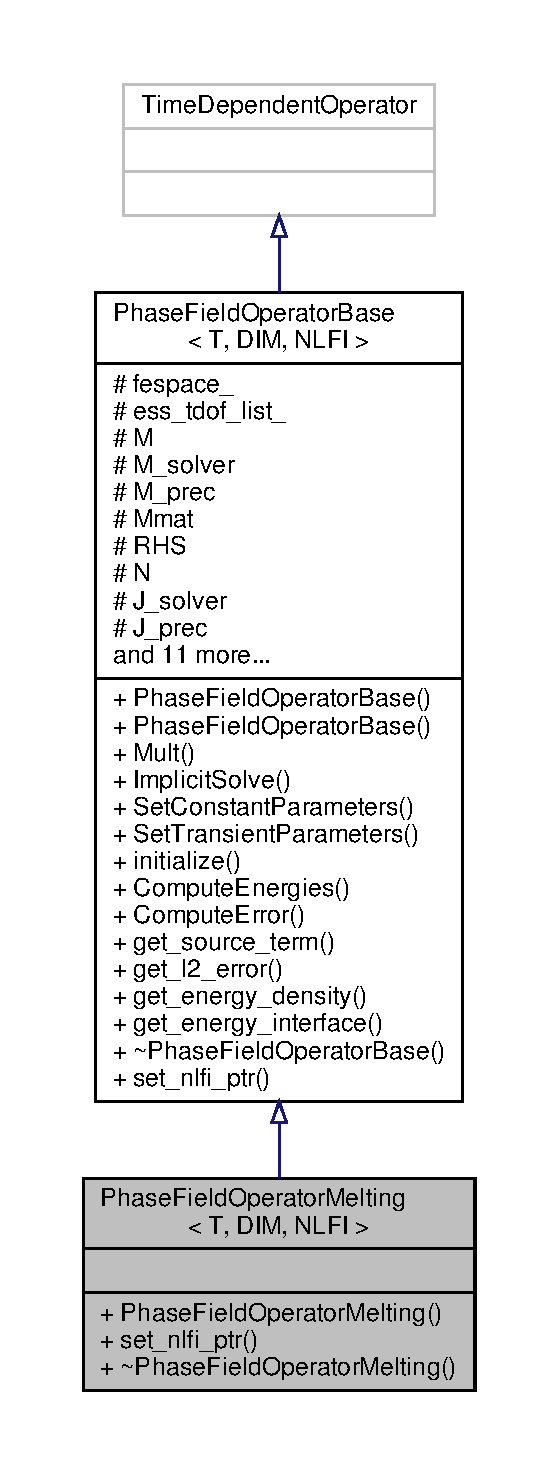
\includegraphics[height=550pt]{classPhaseFieldOperatorMelting__inherit__graph}
\end{center}
\end{figure}


Collaboration diagram for Phase\+Field\+Operator\+Melting$<$ T, D\+IM, N\+L\+FI $>$\+:\nopagebreak
\begin{figure}[H]
\begin{center}
\leavevmode
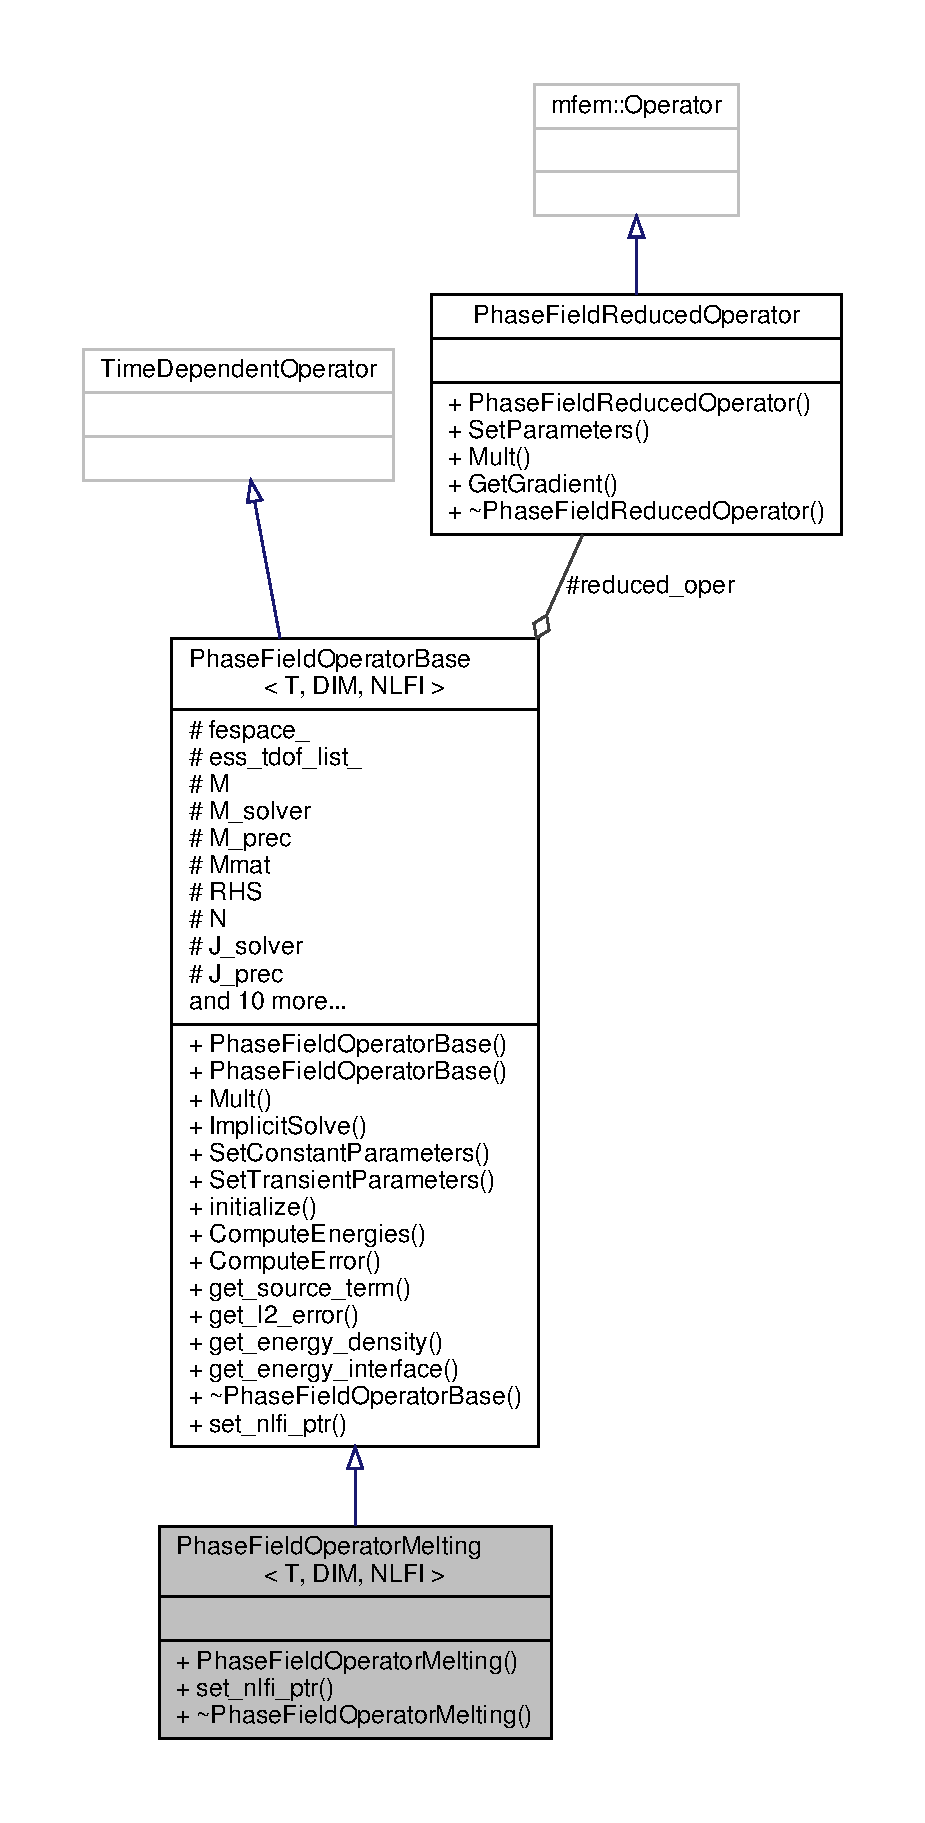
\includegraphics[height=550pt]{classPhaseFieldOperatorMelting__coll__graph}
\end{center}
\end{figure}
\subsection*{Public Member Functions}
\begin{DoxyCompactItemize}
\item 
\hyperlink{classPhaseFieldOperatorMelting_af5647432ef045bf3afd99400640ec233}{Phase\+Field\+Operator\+Melting} (\hyperlink{classSpatialDiscretization}{Spatial\+Discretization}$<$ T, D\+IM $>$ $\ast$spatial, const \hyperlink{classParameters}{Parameters} \&params, \hyperlink{classVariables}{Variables}$<$ T, D\+IM $>$ \&vars)
\begin{DoxyCompactList}\small\item\em Construct a new Phase Field Operator\+:\+: Phase Field Operator object. \end{DoxyCompactList}\item 
N\+L\+FI $\ast$ \hyperlink{classPhaseFieldOperatorMelting_a0235f90bea5d33ab4567cf4ff9e3ce83}{set\+\_\+nlfi\+\_\+ptr} (const double dt, const mfem\+::\+Vector \&u) override
\begin{DoxyCompactList}\small\item\em Set the Non\+Linear\+Form\+Integrator dedicated to melting coupling. \end{DoxyCompactList}\item 
virtual \hyperlink{classPhaseFieldOperatorMelting_af2538e5e548c4dc24ffeb7262d3e8330}{$\sim$\+Phase\+Field\+Operator\+Melting} ()
\begin{DoxyCompactList}\small\item\em Destroy the Phase Field Operator Melting$<$ T,  D\+I\+M,  N\+L\+F\+I$>$\+:\+: Phase Field Operator Melting object. \end{DoxyCompactList}\item 
virtual void \hyperlink{classPhaseFieldOperatorBase_a55a314426a0d9bbb181cb5d35e8f76e9}{Mult} (const mfem\+::\+Vector \&u, mfem\+::\+Vector \&du\+\_\+dt) const
\begin{DoxyCompactList}\small\item\em Compute the right-\/hand side of the O\+DE system. \end{DoxyCompactList}\item 
virtual void \hyperlink{classPhaseFieldOperatorBase_ac1be84d201e35ba329090cdda6a4bfc5}{Implicit\+Solve} (const double dt, const mfem\+::\+Vector \&u, mfem\+::\+Vector \&k)
\begin{DoxyCompactList}\small\item\em Solve the Backward-\/\+Euler equation\+: k = f(phi + dt$\ast$k, t), for the unknown k. \end{DoxyCompactList}\item 
void \hyperlink{classPhaseFieldOperatorBase_ae28add1cf3731d10726a9665862a725b}{Set\+Constant\+Parameters} (const double dt, mfem\+::\+Vector \&u)
\begin{DoxyCompactList}\small\item\em Set current dt, unk values -\/ needed to compute action and Jacobian. \end{DoxyCompactList}\item 
void \hyperlink{classPhaseFieldOperatorBase_a07fb8bcd8791bb712681379c160c1ad6}{Set\+Transient\+Parameters} (const double dt, const mfem\+::\+Vector \&u)
\begin{DoxyCompactList}\small\item\em Set current dt, unk values -\/ needed to compute action and Jacobian. solution\+\_\+coef. \end{DoxyCompactList}\item 
void \hyperlink{classPhaseFieldOperatorBase_a4a85f7d2ece328d8fdb8895a2b76bd0a}{initialize} (const double \&initial\+\_\+time)
\begin{DoxyCompactList}\small\item\em Initialization stage. \end{DoxyCompactList}\item 
void \hyperlink{classPhaseFieldOperatorBase_ac313363a74691d6b500191ff475b57fb}{Compute\+Energies} (const std\+::tuple$<$ int, double, double $>$ \&iter, const mfem\+::\+Vector \&u)
\begin{DoxyCompactList}\small\item\em Compute Phase-\/field Energies. \end{DoxyCompactList}\item 
void \hyperlink{classPhaseFieldOperatorBase_ae2166b96b4d740e05c5dd1ca36e9fc8c}{Compute\+Error} (const std\+::tuple$<$ int, double, double $>$ \&iter, const mfem\+::\+Vector \&u, std\+::function$<$ double(const mfem\+::\+Vector \&, double)$>$ solution\+\_\+func)
\begin{DoxyCompactList}\small\item\em Compute L2 error. \end{DoxyCompactList}\item 
void \hyperlink{classPhaseFieldOperatorBase_ade4aaf43e627fdc8b2a3690839e225d3}{get\+\_\+source\+\_\+term} (mfem\+::\+Vector \&source\+\_\+term) const
\begin{DoxyCompactList}\small\item\em get the source term \end{DoxyCompactList}\item 
const std\+::map$<$ std\+::tuple$<$ int, double, double $>$, double $>$ \hyperlink{classPhaseFieldOperatorBase_adc993d94274e82bc06f9555fbecbd310}{get\+\_\+l2\+\_\+error} () const
\begin{DoxyCompactList}\small\item\em Get a value of a map of L2 errors at a given iteration. \end{DoxyCompactList}\item 
const std\+::map$<$ std\+::tuple$<$ int, double, double $>$, double $>$ \hyperlink{classPhaseFieldOperatorBase_a8428da5d747f60f7ccbd79c879ca8d25}{get\+\_\+energy\+\_\+density} () const
\begin{DoxyCompactList}\small\item\em Get a of a map of interfacial energy at a given iteration. \end{DoxyCompactList}\item 
const std\+::map$<$ std\+::tuple$<$ int, double, double $>$, double $>$ \hyperlink{classPhaseFieldOperatorBase_ac194823660f85a12d8edcf4520bbc025}{get\+\_\+energy\+\_\+interface} () const
\begin{DoxyCompactList}\small\item\em Get a of a map of interfacial energy at a given iteration. \end{DoxyCompactList}\end{DoxyCompactItemize}
\subsection*{Protected Attributes}
\begin{DoxyCompactItemize}
\item 
\mbox{\Hypertarget{classPhaseFieldOperatorBase_ac8697ec5f9f8b2098f695403b7e7d32c}\label{classPhaseFieldOperatorBase_ac8697ec5f9f8b2098f695403b7e7d32c}} 
mfem\+::\+Finite\+Element\+Space $\ast$ {\bfseries fespace\+\_\+}
\item 
\mbox{\Hypertarget{classPhaseFieldOperatorBase_aef9d79b193e695484fc8ece8280a3c6e}\label{classPhaseFieldOperatorBase_aef9d79b193e695484fc8ece8280a3c6e}} 
mfem\+::\+Array$<$ int $>$ {\bfseries ess\+\_\+tdof\+\_\+list\+\_\+}
\item 
\mbox{\Hypertarget{classPhaseFieldOperatorBase_ac59727af25abdd5a0b0eff6a7e766ed2}\label{classPhaseFieldOperatorBase_ac59727af25abdd5a0b0eff6a7e766ed2}} 
mfem\+::\+Bilinear\+Form $\ast$ {\bfseries M}
\item 
\mbox{\Hypertarget{classPhaseFieldOperatorBase_abae6aa970af1afee541f399716c84459}\label{classPhaseFieldOperatorBase_abae6aa970af1afee541f399716c84459}} 
mfem\+::\+C\+G\+Solver {\bfseries M\+\_\+solver}
\item 
\mbox{\Hypertarget{classPhaseFieldOperatorBase_ae0ff8b7ef560d3bde9b6ba13585f57bd}\label{classPhaseFieldOperatorBase_ae0ff8b7ef560d3bde9b6ba13585f57bd}} 
mfem\+::\+D\+Smoother {\bfseries M\+\_\+prec}
\item 
\mbox{\Hypertarget{classPhaseFieldOperatorBase_a3623bbe799103af42de43d798bb3e928}\label{classPhaseFieldOperatorBase_a3623bbe799103af42de43d798bb3e928}} 
mfem\+::\+Sparse\+Matrix {\bfseries Mmat}
\item 
\mbox{\Hypertarget{classPhaseFieldOperatorBase_ab4ba4f88819f656ce8f6dddee6ded24f}\label{classPhaseFieldOperatorBase_ab4ba4f88819f656ce8f6dddee6ded24f}} 
mfem\+::\+Linear\+Form $\ast$ {\bfseries R\+HS}
\item 
\mbox{\Hypertarget{classPhaseFieldOperatorBase_a235f1d2f65754932ca9f1fbfd7f91d91}\label{classPhaseFieldOperatorBase_a235f1d2f65754932ca9f1fbfd7f91d91}} 
mfem\+::\+Nonlinear\+Form $\ast$ {\bfseries N}
\item 
\mbox{\Hypertarget{classPhaseFieldOperatorBase_af0cc6c282ae76674384e3d6a87aa88d9}\label{classPhaseFieldOperatorBase_af0cc6c282ae76674384e3d6a87aa88d9}} 
mfem\+::\+Solver $\ast$ {\bfseries J\+\_\+solver}
\item 
\mbox{\Hypertarget{classPhaseFieldOperatorBase_ab907d8e1cbd9d399959064f8fed3c3e6}\label{classPhaseFieldOperatorBase_ab907d8e1cbd9d399959064f8fed3c3e6}} 
mfem\+::\+Solver $\ast$ {\bfseries J\+\_\+prec}
\item 
\mbox{\Hypertarget{classPhaseFieldOperatorBase_ace8edd3371a4b1b1adaf22a36ad2041a}\label{classPhaseFieldOperatorBase_ace8edd3371a4b1b1adaf22a36ad2041a}} 
\hyperlink{classBoundaryConditions}{Boundary\+Conditions}$<$ T, D\+IM $>$ $\ast$ {\bfseries bcs\+\_\+}
\item 
\mbox{\Hypertarget{classPhaseFieldOperatorBase_a7613689c7c934e661ec287b7b878c9d2}\label{classPhaseFieldOperatorBase_a7613689c7c934e661ec287b7b878c9d2}} 
\hyperlink{classVariables}{Variables}$<$ T, D\+IM $>$ {\bfseries vars\+\_\+}
\item 
\mbox{\Hypertarget{classPhaseFieldOperatorBase_ae643a34ec21563a1aa1e0baee30beb30}\label{classPhaseFieldOperatorBase_ae643a34ec21563a1aa1e0baee30beb30}} 
mfem\+::\+Newton\+Solver {\bfseries newton\+\_\+solver\+\_\+}
\item 
\hyperlink{classPhaseFieldReducedOperator}{Phase\+Field\+Reduced\+Operator} $\ast$ \hyperlink{classPhaseFieldOperatorBase_a010a3da035afe945635288cc0ab2f0b5}{reduced\+\_\+oper}
\item 
\mbox{\Hypertarget{classPhaseFieldOperatorBase_aaa799d0dbf5d04e158f276cc3e0a32cc}\label{classPhaseFieldOperatorBase_aaa799d0dbf5d04e158f276cc3e0a32cc}} 
double {\bfseries mobility\+\_\+coeff\+\_\+}
\item 
\mbox{\Hypertarget{classPhaseFieldOperatorBase_a275f0cce177c9cd3c2cced2771b8f702}\label{classPhaseFieldOperatorBase_a275f0cce177c9cd3c2cced2771b8f702}} 
double {\bfseries omega\+\_\+}
\item 
\mbox{\Hypertarget{classPhaseFieldOperatorBase_a55ca706b0f6f4ee16eb1c27523569a2c}\label{classPhaseFieldOperatorBase_a55ca706b0f6f4ee16eb1c27523569a2c}} 
double {\bfseries lambda\+\_\+}
\item 
\mbox{\Hypertarget{classPhaseFieldOperatorBase_a1cc7b7915970f927c7e3bde1d06b9412}\label{classPhaseFieldOperatorBase_a1cc7b7915970f927c7e3bde1d06b9412}} 
std\+::function$<$ double(const mfem\+::\+Vector \&, double)$>$ {\bfseries src\+\_\+func\+\_\+}
\item 
\mbox{\Hypertarget{classPhaseFieldOperatorBase_ac7c9e3138a6324901705e74da62421ea}\label{classPhaseFieldOperatorBase_ac7c9e3138a6324901705e74da62421ea}} 
double {\bfseries current\+\_\+dt\+\_\+}
\item 
\mbox{\Hypertarget{classPhaseFieldOperatorBase_a67fca8849db8e5659f633a2c0df694b7}\label{classPhaseFieldOperatorBase_a67fca8849db8e5659f633a2c0df694b7}} 
mfem\+::\+Vector {\bfseries z}
\item 
\mbox{\Hypertarget{classPhaseFieldOperatorBase_aefbc006a9f535e2ab69a9a8964e2b159}\label{classPhaseFieldOperatorBase_aefbc006a9f535e2ab69a9a8964e2b159}} 
std\+::string {\bfseries source\+\_\+term\+\_\+name\+\_\+}
\end{DoxyCompactItemize}


\subsection{Detailed Description}
\subsubsection*{template$<$class T, int D\+IM, class N\+L\+FI$>$\newline
class Phase\+Field\+Operator\+Melting$<$ T, D\+I\+M, N\+L\+F\+I $>$}

\hyperlink{classPhaseFieldOperatorMelting}{Phase\+Field\+Operator\+Melting} class. 

Definition at line 46 of file Phase\+Field\+Operator\+Melting.\+hpp.



\subsection{Constructor \& Destructor Documentation}
\mbox{\Hypertarget{classPhaseFieldOperatorMelting_af5647432ef045bf3afd99400640ec233}\label{classPhaseFieldOperatorMelting_af5647432ef045bf3afd99400640ec233}} 
\index{Phase\+Field\+Operator\+Melting@{Phase\+Field\+Operator\+Melting}!Phase\+Field\+Operator\+Melting@{Phase\+Field\+Operator\+Melting}}
\index{Phase\+Field\+Operator\+Melting@{Phase\+Field\+Operator\+Melting}!Phase\+Field\+Operator\+Melting@{Phase\+Field\+Operator\+Melting}}
\subsubsection{\texorpdfstring{Phase\+Field\+Operator\+Melting()}{PhaseFieldOperatorMelting()}}
{\footnotesize\ttfamily template$<$class T , int D\+IM, class N\+L\+FI $>$ \\
\hyperlink{classPhaseFieldOperatorMelting}{Phase\+Field\+Operator\+Melting}$<$ T, D\+IM, N\+L\+FI $>$\+::\hyperlink{classPhaseFieldOperatorMelting}{Phase\+Field\+Operator\+Melting} (\begin{DoxyParamCaption}\item[{\hyperlink{classSpatialDiscretization}{Spatial\+Discretization}$<$ T, D\+IM $>$ $\ast$}]{spatial,  }\item[{const \hyperlink{classParameters}{Parameters} \&}]{params,  }\item[{\hyperlink{classVariables}{Variables}$<$ T, D\+IM $>$ \&}]{vars }\end{DoxyParamCaption})}



Construct a new Phase Field Operator\+:\+: Phase Field Operator object. 


\begin{DoxyParams}{Parameters}
{\em fespace} & Finite Element space \\
\hline
{\em params} & list of \hyperlink{classParameters}{Parameters} \\
\hline
{\em u} & unknown vector \\
\hline
\end{DoxyParams}


Definition at line 68 of file Phase\+Field\+Operator\+Melting.\+hpp.


\begin{DoxyCode}
70     : \hyperlink{classPhaseFieldOperatorBase}{PhaseFieldOperatorBase<T, DIM, NLFI>}(spatial, params, vars) \{\}
\end{DoxyCode}
\mbox{\Hypertarget{classPhaseFieldOperatorMelting_af2538e5e548c4dc24ffeb7262d3e8330}\label{classPhaseFieldOperatorMelting_af2538e5e548c4dc24ffeb7262d3e8330}} 
\index{Phase\+Field\+Operator\+Melting@{Phase\+Field\+Operator\+Melting}!````~Phase\+Field\+Operator\+Melting@{$\sim$\+Phase\+Field\+Operator\+Melting}}
\index{````~Phase\+Field\+Operator\+Melting@{$\sim$\+Phase\+Field\+Operator\+Melting}!Phase\+Field\+Operator\+Melting@{Phase\+Field\+Operator\+Melting}}
\subsubsection{\texorpdfstring{$\sim$\+Phase\+Field\+Operator\+Melting()}{~PhaseFieldOperatorMelting()}}
{\footnotesize\ttfamily template$<$class T , int D\+IM, class N\+L\+FI $>$ \\
\hyperlink{classPhaseFieldOperatorMelting}{Phase\+Field\+Operator\+Melting}$<$ T, D\+IM, N\+L\+FI $>$\+::$\sim$\hyperlink{classPhaseFieldOperatorMelting}{Phase\+Field\+Operator\+Melting} (\begin{DoxyParamCaption}{ }\end{DoxyParamCaption})\hspace{0.3cm}{\ttfamily [virtual]}}



Destroy the Phase Field Operator Melting$<$ T,  D\+I\+M,  N\+L\+F\+I$>$\+:\+: Phase Field Operator Melting object. 


\begin{DoxyTemplParams}{Template Parameters}
{\em T} & \\
\hline
{\em D\+IM} & \\
\hline
\end{DoxyTemplParams}


Definition at line 103 of file Phase\+Field\+Operator\+Melting.\+hpp.


\begin{DoxyCode}
103 \{\}
\end{DoxyCode}


\subsection{Member Function Documentation}
\mbox{\Hypertarget{classPhaseFieldOperatorBase_ac313363a74691d6b500191ff475b57fb}\label{classPhaseFieldOperatorBase_ac313363a74691d6b500191ff475b57fb}} 
\index{Phase\+Field\+Operator\+Melting@{Phase\+Field\+Operator\+Melting}!Compute\+Energies@{Compute\+Energies}}
\index{Compute\+Energies@{Compute\+Energies}!Phase\+Field\+Operator\+Melting@{Phase\+Field\+Operator\+Melting}}
\subsubsection{\texorpdfstring{Compute\+Energies()}{ComputeEnergies()}}
{\footnotesize\ttfamily template$<$class T , int D\+IM, class N\+L\+FI $>$ \\
void \hyperlink{classPhaseFieldOperatorBase}{Phase\+Field\+Operator\+Base}$<$ T, D\+IM, N\+L\+FI $>$\+::Compute\+Energies (\begin{DoxyParamCaption}\item[{const std\+::tuple$<$ int, double, double $>$ \&}]{iter,  }\item[{const mfem\+::\+Vector \&}]{u }\end{DoxyParamCaption})\hspace{0.3cm}{\ttfamily [inherited]}}



Compute Phase-\/field Energies. 


\begin{DoxyParams}{Parameters}
{\em u} & unknown vector \\
\hline
\end{DoxyParams}
\begin{DoxyReturn}{Returns}
const double 
\end{DoxyReturn}


Definition at line 338 of file Phase\+Field\+Operator\+Base.\+hpp.


\begin{DoxyCode}
339                                                                     \{
340   mfem::GridFunction un\_gf(this->fespace\_);
341   un\_gf.SetFromTrueDofs(u);
342   mfem::GridFunction gf(this->fespace\_);
343   \hyperlink{classEnergyCoefficient}{EnergyCoefficient} g(&un\_gf, 0.5 * this->lambda\_, this->omega\_);
344   gf.ProjectCoefficient(g);
345   mfem::GridFunction sigf(this->fespace\_);
346   \hyperlink{classEnergyCoefficient}{EnergyCoefficient} sig(&un\_gf, this->lambda\_, 0.);
347   sigf.ProjectCoefficient(sig);
348 
349   \textcolor{comment}{// Calcul de l'intégrale de l'objet FunctionCoefficient sur le domaine}
350   mfem::ConstantCoefficient zero(0.);
351   \textcolor{keyword}{const} \textcolor{keyword}{auto} energy = gf.ComputeL1Error(zero);
352   this->energy\_density\_.try\_emplace(iter, energy);
353   \textcolor{keyword}{const} \textcolor{keyword}{auto} interfacial\_energy = sigf.ComputeL1Error(zero);
354   this->energy\_interface\_.try\_emplace(iter, interfacial\_energy);
355 \}
\end{DoxyCode}
\mbox{\Hypertarget{classPhaseFieldOperatorBase_ae2166b96b4d740e05c5dd1ca36e9fc8c}\label{classPhaseFieldOperatorBase_ae2166b96b4d740e05c5dd1ca36e9fc8c}} 
\index{Phase\+Field\+Operator\+Melting@{Phase\+Field\+Operator\+Melting}!Compute\+Error@{Compute\+Error}}
\index{Compute\+Error@{Compute\+Error}!Phase\+Field\+Operator\+Melting@{Phase\+Field\+Operator\+Melting}}
\subsubsection{\texorpdfstring{Compute\+Error()}{ComputeError()}}
{\footnotesize\ttfamily template$<$class T , int D\+IM, class N\+L\+FI $>$ \\
void \hyperlink{classPhaseFieldOperatorBase}{Phase\+Field\+Operator\+Base}$<$ T, D\+IM, N\+L\+FI $>$\+::Compute\+Error (\begin{DoxyParamCaption}\item[{const std\+::tuple$<$ int, double, double $>$ \&}]{iter,  }\item[{const mfem\+::\+Vector \&}]{u,  }\item[{std\+::function$<$ double(const mfem\+::\+Vector \&, double)$>$}]{solution\+\_\+func }\end{DoxyParamCaption})\hspace{0.3cm}{\ttfamily [inherited]}}



Compute L2 error. 


\begin{DoxyParams}{Parameters}
{\em u} & unknown vector \\
\hline
\end{DoxyParams}
\begin{DoxyReturn}{Returns}
const double 
\end{DoxyReturn}


Definition at line 364 of file Phase\+Field\+Operator\+Base.\+hpp.


\begin{DoxyCode}
366                                                                    \{
367   mfem::GridFunction gf(this->fespace\_);
368   gf.SetFromTrueDofs(u);
369   mfem::FunctionCoefficient solution\_coef(solution\_func);
370   solution\_coef.SetTime(this->GetTime());
371   \textcolor{keyword}{const} \textcolor{keyword}{auto} error = gf.ComputeL2Error(solution\_coef);
372   this->error\_l2\_.try\_emplace(iter, error);
373 \}
\end{DoxyCode}
\mbox{\Hypertarget{classPhaseFieldOperatorBase_a8428da5d747f60f7ccbd79c879ca8d25}\label{classPhaseFieldOperatorBase_a8428da5d747f60f7ccbd79c879ca8d25}} 
\index{Phase\+Field\+Operator\+Melting@{Phase\+Field\+Operator\+Melting}!get\+\_\+energy\+\_\+density@{get\+\_\+energy\+\_\+density}}
\index{get\+\_\+energy\+\_\+density@{get\+\_\+energy\+\_\+density}!Phase\+Field\+Operator\+Melting@{Phase\+Field\+Operator\+Melting}}
\subsubsection{\texorpdfstring{get\+\_\+energy\+\_\+density()}{get\_energy\_density()}}
{\footnotesize\ttfamily template$<$class T , int D\+IM, class N\+L\+FI $>$ \\
const std\+::map$<$ std\+::tuple$<$ int, double, double $>$, double $>$ \hyperlink{classPhaseFieldOperatorBase}{Phase\+Field\+Operator\+Base}$<$ T, D\+IM, N\+L\+FI $>$\+::get\+\_\+energy\+\_\+density (\begin{DoxyParamCaption}{ }\end{DoxyParamCaption}) const\hspace{0.3cm}{\ttfamily [inherited]}}



Get a of a map of interfacial energy at a given iteration. 


\begin{DoxyTemplParams}{Template Parameters}
{\em T} & \\
\hline
{\em D\+IM} & \\
\hline
{\em N\+L\+FI} & \\
\hline
\end{DoxyTemplParams}
\begin{DoxyReturn}{Returns}
const std\+::map$<$std\+::tuple$<$int, double, double$>$, double$>$ 
\end{DoxyReturn}


Definition at line 417 of file Phase\+Field\+Operator\+Base.\+hpp.


\begin{DoxyCode}
417                                                                \{
418   \textcolor{keywordflow}{return} this->energy\_density\_;
419 \}
\end{DoxyCode}
\mbox{\Hypertarget{classPhaseFieldOperatorBase_ac194823660f85a12d8edcf4520bbc025}\label{classPhaseFieldOperatorBase_ac194823660f85a12d8edcf4520bbc025}} 
\index{Phase\+Field\+Operator\+Melting@{Phase\+Field\+Operator\+Melting}!get\+\_\+energy\+\_\+interface@{get\+\_\+energy\+\_\+interface}}
\index{get\+\_\+energy\+\_\+interface@{get\+\_\+energy\+\_\+interface}!Phase\+Field\+Operator\+Melting@{Phase\+Field\+Operator\+Melting}}
\subsubsection{\texorpdfstring{get\+\_\+energy\+\_\+interface()}{get\_energy\_interface()}}
{\footnotesize\ttfamily template$<$class T , int D\+IM, class N\+L\+FI $>$ \\
const std\+::map$<$ std\+::tuple$<$ int, double, double $>$, double $>$ \hyperlink{classPhaseFieldOperatorBase}{Phase\+Field\+Operator\+Base}$<$ T, D\+IM, N\+L\+FI $>$\+::get\+\_\+energy\+\_\+interface (\begin{DoxyParamCaption}{ }\end{DoxyParamCaption}) const\hspace{0.3cm}{\ttfamily [inherited]}}



Get a of a map of interfacial energy at a given iteration. 


\begin{DoxyTemplParams}{Template Parameters}
{\em T} & \\
\hline
{\em D\+IM} & \\
\hline
{\em N\+L\+FI} & \\
\hline
\end{DoxyTemplParams}
\begin{DoxyReturn}{Returns}
const std\+::map$<$std\+::tuple$<$int, double, double$>$, double$>$ 
\end{DoxyReturn}


Definition at line 431 of file Phase\+Field\+Operator\+Base.\+hpp.


\begin{DoxyCode}
431                                                                  \{
432   \textcolor{keywordflow}{return} this->energy\_interface\_;
433 \}
\end{DoxyCode}
\mbox{\Hypertarget{classPhaseFieldOperatorBase_adc993d94274e82bc06f9555fbecbd310}\label{classPhaseFieldOperatorBase_adc993d94274e82bc06f9555fbecbd310}} 
\index{Phase\+Field\+Operator\+Melting@{Phase\+Field\+Operator\+Melting}!get\+\_\+l2\+\_\+error@{get\+\_\+l2\+\_\+error}}
\index{get\+\_\+l2\+\_\+error@{get\+\_\+l2\+\_\+error}!Phase\+Field\+Operator\+Melting@{Phase\+Field\+Operator\+Melting}}
\subsubsection{\texorpdfstring{get\+\_\+l2\+\_\+error()}{get\_l2\_error()}}
{\footnotesize\ttfamily template$<$class T , int D\+IM, class N\+L\+FI $>$ \\
const std\+::map$<$ std\+::tuple$<$ int, double, double $>$, double $>$ \hyperlink{classPhaseFieldOperatorBase}{Phase\+Field\+Operator\+Base}$<$ T, D\+IM, N\+L\+FI $>$\+::get\+\_\+l2\+\_\+error (\begin{DoxyParamCaption}{ }\end{DoxyParamCaption}) const\hspace{0.3cm}{\ttfamily [inherited]}}



Get a value of a map of L2 errors at a given iteration. 


\begin{DoxyTemplParams}{Template Parameters}
{\em T} & \\
\hline
{\em D\+IM} & \\
\hline
{\em N\+L\+FI} & \\
\hline
\end{DoxyTemplParams}

\begin{DoxyParams}{Parameters}
{\em iter} & \\
\hline
\end{DoxyParams}
\begin{DoxyReturn}{Returns}
const std\+::map$<$std\+::tuple$<$int, double, double$>$, double$>$ 
\end{DoxyReturn}


Definition at line 403 of file Phase\+Field\+Operator\+Base.\+hpp.


\begin{DoxyCode}
403                                                          \{
404   \textcolor{keywordflow}{return} this->error\_l2\_;
405 \}
\end{DoxyCode}
\mbox{\Hypertarget{classPhaseFieldOperatorBase_ade4aaf43e627fdc8b2a3690839e225d3}\label{classPhaseFieldOperatorBase_ade4aaf43e627fdc8b2a3690839e225d3}} 
\index{Phase\+Field\+Operator\+Melting@{Phase\+Field\+Operator\+Melting}!get\+\_\+source\+\_\+term@{get\+\_\+source\+\_\+term}}
\index{get\+\_\+source\+\_\+term@{get\+\_\+source\+\_\+term}!Phase\+Field\+Operator\+Melting@{Phase\+Field\+Operator\+Melting}}
\subsubsection{\texorpdfstring{get\+\_\+source\+\_\+term()}{get\_source\_term()}}
{\footnotesize\ttfamily template$<$class T , int D\+IM, class N\+L\+FI $>$ \\
void \hyperlink{classPhaseFieldOperatorBase}{Phase\+Field\+Operator\+Base}$<$ T, D\+IM, N\+L\+FI $>$\+::get\+\_\+source\+\_\+term (\begin{DoxyParamCaption}\item[{mfem\+::\+Vector \&}]{source\+\_\+term }\end{DoxyParamCaption}) const\hspace{0.3cm}{\ttfamily [inherited]}}



get the source term 


\begin{DoxyTemplParams}{Template Parameters}
{\em T} & \\
\hline
{\em D\+IM} & \\
\hline
{\em N\+L\+FI} & \\
\hline
\end{DoxyTemplParams}


Definition at line 383 of file Phase\+Field\+Operator\+Base.\+hpp.



Referenced by Phase\+Field\+Operator\+Base$<$ T, D\+I\+M, N\+L\+F\+I $>$\+::\+Implicit\+Solve(), and Phase\+Field\+Operator\+Base$<$ T, D\+I\+M, N\+L\+F\+I $>$\+::\+Mult().


\begin{DoxyCode}
383                                                                                         \{
384   std::shared\_ptr<mfem::LinearForm> RHSS(\textcolor{keyword}{new} mfem::LinearForm(this->fespace\_));
385   mfem::FunctionCoefficient src(this->src\_func\_);
386   src.SetTime(this->GetTime());
387   RHSS->AddDomainIntegrator(\textcolor{keyword}{new} mfem::DomainLFIntegrator(src));
388   RHSS->Assemble();
389   source\_term = *RHSS.get();
390 \}
\end{DoxyCode}
\mbox{\Hypertarget{classPhaseFieldOperatorBase_ac1be84d201e35ba329090cdda6a4bfc5}\label{classPhaseFieldOperatorBase_ac1be84d201e35ba329090cdda6a4bfc5}} 
\index{Phase\+Field\+Operator\+Melting@{Phase\+Field\+Operator\+Melting}!Implicit\+Solve@{Implicit\+Solve}}
\index{Implicit\+Solve@{Implicit\+Solve}!Phase\+Field\+Operator\+Melting@{Phase\+Field\+Operator\+Melting}}
\subsubsection{\texorpdfstring{Implicit\+Solve()}{ImplicitSolve()}}
{\footnotesize\ttfamily template$<$class T , int D\+IM, class N\+L\+FI $>$ \\
void \hyperlink{classPhaseFieldOperatorBase}{Phase\+Field\+Operator\+Base}$<$ T, D\+IM, N\+L\+FI $>$\+::Implicit\+Solve (\begin{DoxyParamCaption}\item[{const double}]{dt,  }\item[{const mfem\+::\+Vector \&}]{u,  }\item[{mfem\+::\+Vector \&}]{du\+\_\+dt }\end{DoxyParamCaption})\hspace{0.3cm}{\ttfamily [virtual]}, {\ttfamily [inherited]}}



Solve the Backward-\/\+Euler equation\+: k = f(phi + dt$\ast$k, t), for the unknown k. 

Solve the Backward-\/\+Euler equation\+: k = f(u + dt$\ast$k, t), for the unknown k. This is the only requirement for high-\/order S\+D\+I\+RK implicit integration.


\begin{DoxyParams}{Parameters}
{\em dt} & current time step \\
\hline
{\em u} & unknown vector \\
\hline
{\em du\+\_\+dt} & unkwon time derivative vector \\
\hline
\end{DoxyParams}


Definition at line 302 of file Phase\+Field\+Operator\+Base.\+hpp.



References Phase\+Field\+Operator\+Base$<$ T, D\+I\+M, N\+L\+F\+I $>$\+::get\+\_\+source\+\_\+term(), Boundary\+Conditions$<$ T, D\+I\+M $>$\+::\+Set\+Boundary\+Conditions(), Phase\+Field\+Reduced\+Operator\+::\+Set\+Parameters(), and Phase\+Field\+Operator\+Base$<$ T, D\+I\+M, N\+L\+F\+I $>$\+::\+Set\+Transient\+Parameters().


\begin{DoxyCode}
303                                                                             \{
304   \textcolor{keyword}{const} \textcolor{keyword}{auto} sc = height;
305   mfem::Vector v(u.GetData(), sc);
306   mfem::Vector dv\_dt(du\_dt.GetData(), sc);
307   \textcolor{comment}{// // Solve the equation:}
308   \textcolor{comment}{// //    du\_dt = M^\{-1\}*[-K(u + dt*du\_dt)]}
309   \textcolor{comment}{// // for du\_dt}
310 
311   this->bcs\_->SetBoundaryConditions(v);
312   this->\hyperlink{classPhaseFieldOperatorBase_a07fb8bcd8791bb712681379c160c1ad6}{SetTransientParameters}(dt, v);
313 
314   \hyperlink{classPhaseFieldOperatorBase_a010a3da035afe945635288cc0ab2f0b5}{reduced\_oper}->\hyperlink{classPhaseFieldReducedOperator_aaaa55d33260a9dc98051bd97f916bf46}{SetParameters}(dt, &v);
315 
316   \textcolor{comment}{// Source term}
317   mfem::Vector source\_term;
318   \textcolor{keywordflow}{if} (!this->source\_term\_name\_.empty()) \{
319     this->\hyperlink{classPhaseFieldOperatorBase_ade4aaf43e627fdc8b2a3690839e225d3}{get\_source\_term}(source\_term);
320   \}
321 
322   dv\_dt = v;
323   dv\_dt *= (1. / dt);
324   this->newton\_solver\_.Mult(source\_term, dv\_dt);
325   dv\_dt.SetSubVector(this->ess\_tdof\_list\_, 0.0);  \textcolor{comment}{// pour  Dirichlet ... uniquement?}
326   \textcolor{comment}{// std::cout << " PhaseFieldOperatorBase this->newton\_solver\_->Mult " << std::endl;}
327 
328   MFEM\_VERIFY(this->newton\_solver\_.GetConverged(), \textcolor{stringliteral}{"Nonlinear solver did not converge."});
329 \}
\end{DoxyCode}
\mbox{\Hypertarget{classPhaseFieldOperatorBase_a4a85f7d2ece328d8fdb8895a2b76bd0a}\label{classPhaseFieldOperatorBase_a4a85f7d2ece328d8fdb8895a2b76bd0a}} 
\index{Phase\+Field\+Operator\+Melting@{Phase\+Field\+Operator\+Melting}!initialize@{initialize}}
\index{initialize@{initialize}!Phase\+Field\+Operator\+Melting@{Phase\+Field\+Operator\+Melting}}
\subsubsection{\texorpdfstring{initialize()}{initialize()}}
{\footnotesize\ttfamily template$<$class T , int D\+IM, class N\+L\+FI $>$ \\
void \hyperlink{classPhaseFieldOperatorBase}{Phase\+Field\+Operator\+Base}$<$ T, D\+IM, N\+L\+FI $>$\+::initialize (\begin{DoxyParamCaption}\item[{const double \&}]{initial\+\_\+time }\end{DoxyParamCaption})\hspace{0.3cm}{\ttfamily [inherited]}}



Initialization stage. 


\begin{DoxyParams}{Parameters}
{\em vv} & \\
\hline
\end{DoxyParams}


Definition at line 186 of file Phase\+Field\+Operator\+Base.\+hpp.



References Variables$<$ T, D\+I\+M $>$\+::get\+\_\+variable(), Boundary\+Conditions$<$ T, D\+I\+M $>$\+::\+Get\+Essential\+Dofs(), Boundary\+Conditions$<$ T, D\+I\+M $>$\+::\+Set\+Boundary\+Conditions(), Phase\+Field\+Operator\+Base$<$ T, D\+I\+M, N\+L\+F\+I $>$\+::\+Set\+Constant\+Parameters(), and Phase\+Field\+Operator\+Base$<$ T, D\+I\+M, N\+L\+F\+I $>$\+::\+Set\+Transient\+Parameters().


\begin{DoxyCode}
186                                                                                 \{
187   this->SetTime(initial\_time);
188   \textcolor{keyword}{auto} &vv = vars\_.get\_variable(\textcolor{stringliteral}{"phi"});
189   \textcolor{keyword}{auto} u = vv.get\_unknown();
190 
191   this->bcs\_ = vv.get\_boundary\_conditions();
192   this->ess\_tdof\_list\_ = this->bcs\_->GetEssentialDofs();
193   this->bcs\_->SetBoundaryConditions(u);
194   this->\hyperlink{classPhaseFieldOperatorBase_ae28add1cf3731d10726a9665862a725b}{SetConstantParameters}(this->current\_dt\_, u);
195   this->\hyperlink{classPhaseFieldOperatorBase_a07fb8bcd8791bb712681379c160c1ad6}{SetTransientParameters}(this->current\_dt\_, u);
196   vv.update(u);
197 \}
\end{DoxyCode}
\mbox{\Hypertarget{classPhaseFieldOperatorBase_a55a314426a0d9bbb181cb5d35e8f76e9}\label{classPhaseFieldOperatorBase_a55a314426a0d9bbb181cb5d35e8f76e9}} 
\index{Phase\+Field\+Operator\+Melting@{Phase\+Field\+Operator\+Melting}!Mult@{Mult}}
\index{Mult@{Mult}!Phase\+Field\+Operator\+Melting@{Phase\+Field\+Operator\+Melting}}
\subsubsection{\texorpdfstring{Mult()}{Mult()}}
{\footnotesize\ttfamily template$<$class T , int D\+IM, class N\+L\+FI $>$ \\
void \hyperlink{classPhaseFieldOperatorBase}{Phase\+Field\+Operator\+Base}$<$ T, D\+IM, N\+L\+FI $>$\+::Mult (\begin{DoxyParamCaption}\item[{const mfem\+::\+Vector \&}]{u,  }\item[{mfem\+::\+Vector \&}]{du\+\_\+dt }\end{DoxyParamCaption}) const\hspace{0.3cm}{\ttfamily [virtual]}, {\ttfamily [inherited]}}



Compute the right-\/hand side of the O\+DE system. 


\begin{DoxyParams}{Parameters}
{\em u} & unknown vector \\
\hline
{\em du\+\_\+dt} & unkwon time derivative vector \\
\hline
\end{DoxyParams}


Definition at line 276 of file Phase\+Field\+Operator\+Base.\+hpp.



References Phase\+Field\+Operator\+Base$<$ T, D\+I\+M, N\+L\+F\+I $>$\+::get\+\_\+source\+\_\+term().


\begin{DoxyCode}
276                                                                                             \{
277   \textcolor{keyword}{const} \textcolor{keyword}{auto} sc = height;
278   mfem::Vector v(u.GetData(), sc);
279   mfem::Vector dv\_dt(du\_dt.GetData(), sc);
280 
281   N->Mult(v, z);
282 
283   \textcolor{comment}{// Source term}
284   \textcolor{keywordflow}{if} (!this->source\_term\_name\_.empty()) \{
285     mfem::Vector source\_term;
286     this->\hyperlink{classPhaseFieldOperatorBase_ade4aaf43e627fdc8b2a3690839e225d3}{get\_source\_term}(source\_term);
287     z -= source\_term;
288   \}
289 
290   z.Neg();  \textcolor{comment}{// z = -z}
291   M\_solver.Mult(z, dv\_dt);
292 \}
\end{DoxyCode}
\mbox{\Hypertarget{classPhaseFieldOperatorMelting_a0235f90bea5d33ab4567cf4ff9e3ce83}\label{classPhaseFieldOperatorMelting_a0235f90bea5d33ab4567cf4ff9e3ce83}} 
\index{Phase\+Field\+Operator\+Melting@{Phase\+Field\+Operator\+Melting}!set\+\_\+nlfi\+\_\+ptr@{set\+\_\+nlfi\+\_\+ptr}}
\index{set\+\_\+nlfi\+\_\+ptr@{set\+\_\+nlfi\+\_\+ptr}!Phase\+Field\+Operator\+Melting@{Phase\+Field\+Operator\+Melting}}
\subsubsection{\texorpdfstring{set\+\_\+nlfi\+\_\+ptr()}{set\_nlfi\_ptr()}}
{\footnotesize\ttfamily template$<$class T , int D\+IM, class N\+L\+FI $>$ \\
N\+L\+FI $\ast$ \hyperlink{classPhaseFieldOperatorMelting}{Phase\+Field\+Operator\+Melting}$<$ T, D\+IM, N\+L\+FI $>$\+::set\+\_\+nlfi\+\_\+ptr (\begin{DoxyParamCaption}\item[{const double}]{dt,  }\item[{const mfem\+::\+Vector \&}]{u }\end{DoxyParamCaption})\hspace{0.3cm}{\ttfamily [override]}, {\ttfamily [virtual]}}



Set the Non\+Linear\+Form\+Integrator dedicated to melting coupling. 


\begin{DoxyTemplParams}{Template Parameters}
{\em T} & \\
\hline
{\em D\+IM} & \\
\hline
\end{DoxyTemplParams}

\begin{DoxyParams}{Parameters}
{\em dt} & \\
\hline
{\em u} & \\
\hline
\end{DoxyParams}
\begin{DoxyReturn}{Returns}
N\+L\+F\+I$\ast$ 
\end{DoxyReturn}


Implements \hyperlink{classPhaseFieldOperatorBase}{Phase\+Field\+Operator\+Base$<$ T, D\+I\+M, N\+L\+F\+I $>$}.



Definition at line 82 of file Phase\+Field\+Operator\+Melting.\+hpp.


\begin{DoxyCode}
83                                                                                  \{
84   mfem::GridFunction un(this->fespace\_);
85   un.SetFromTrueDofs(u);
86   \textcolor{comment}{// PhaseChange Coefficient}
87   \hyperlink{classPhaseChangeCoefficient}{PhaseChangeCoefficient} phase\_change;
88   phase\_change.SetTime(this->GetTime());
89   un.ProjectCoefficient(phase\_change);
90 
91   NLFI *nlfi\_ptr = \textcolor{keyword}{new} NLFI(un, this->omega\_, this->lambda\_, this->mobility\_coeff\_, phase\_change);
92   \textcolor{keywordflow}{return} nlfi\_ptr;
93 \}
\end{DoxyCode}
\mbox{\Hypertarget{classPhaseFieldOperatorBase_ae28add1cf3731d10726a9665862a725b}\label{classPhaseFieldOperatorBase_ae28add1cf3731d10726a9665862a725b}} 
\index{Phase\+Field\+Operator\+Melting@{Phase\+Field\+Operator\+Melting}!Set\+Constant\+Parameters@{Set\+Constant\+Parameters}}
\index{Set\+Constant\+Parameters@{Set\+Constant\+Parameters}!Phase\+Field\+Operator\+Melting@{Phase\+Field\+Operator\+Melting}}
\subsubsection{\texorpdfstring{Set\+Constant\+Parameters()}{SetConstantParameters()}}
{\footnotesize\ttfamily template$<$class T , int D\+IM, class N\+L\+FI $>$ \\
void \hyperlink{classPhaseFieldOperatorBase}{Phase\+Field\+Operator\+Base}$<$ T, D\+IM, N\+L\+FI $>$\+::Set\+Constant\+Parameters (\begin{DoxyParamCaption}\item[{const double}]{dt,  }\item[{mfem\+::\+Vector \&}]{u }\end{DoxyParamCaption})\hspace{0.3cm}{\ttfamily [inherited]}}



Set current dt, unk values -\/ needed to compute action and Jacobian. 


\begin{DoxyParams}{Parameters}
{\em dt} & time-\/step \\
\hline
{\em u} & unknown vector \\
\hline
{\em ess\+\_\+tdof\+\_\+list} & array of dofs \\
\hline
\end{DoxyParams}


Definition at line 250 of file Phase\+Field\+Operator\+Base.\+hpp.



References Utils\+For\+Solvers\+::\+Build\+Solver(), and Utils\+For\+Solvers\+::\+Set\+Solver\+Parameters().



Referenced by Phase\+Field\+Operator\+Base$<$ T, D\+I\+M, N\+L\+F\+I $>$\+::initialize().


\begin{DoxyCode}
250                                                                                                \{
251   \textcolor{keyword}{delete} M;
253   \textcolor{comment}{// Mass matrix (constant)}
255 \textcolor{comment}{}  M = \textcolor{keyword}{new} mfem::BilinearForm(this->fespace\_);
256   M->AddDomainIntegrator(\textcolor{keyword}{new} mfem::MassIntegrator());
257   M->Assemble(0);
258   mfem::SparseMatrix tmp;
259   M->FormSystemMatrix(this->ess\_tdof\_list\_, Mmat);
260   this->ut\_solver\_.\hyperlink{classUtilsForSolvers_a5e352c96817ea210dcf3e080c13d4b1d}{SetSolverParameters}(
261       M\_solver, MassDefaultConstant::print\_level, MassDefaultConstant::iterative\_mode,
262       MassDefaultConstant::iter\_max, MassDefaultConstant::rel\_tol, MassDefaultConstant::abs\_tol);
263   this->ut\_solver\_.\hyperlink{classUtilsForSolvers_a5c76f7ef4f28a5e22f6d07666134aa4d}{BuildSolver}(M\_solver, M\_prec, Mmat);
264 \}
\end{DoxyCode}
\mbox{\Hypertarget{classPhaseFieldOperatorBase_a07fb8bcd8791bb712681379c160c1ad6}\label{classPhaseFieldOperatorBase_a07fb8bcd8791bb712681379c160c1ad6}} 
\index{Phase\+Field\+Operator\+Melting@{Phase\+Field\+Operator\+Melting}!Set\+Transient\+Parameters@{Set\+Transient\+Parameters}}
\index{Set\+Transient\+Parameters@{Set\+Transient\+Parameters}!Phase\+Field\+Operator\+Melting@{Phase\+Field\+Operator\+Melting}}
\subsubsection{\texorpdfstring{Set\+Transient\+Parameters()}{SetTransientParameters()}}
{\footnotesize\ttfamily template$<$class T , int D\+IM, class N\+L\+FI $>$ \\
void \hyperlink{classPhaseFieldOperatorBase}{Phase\+Field\+Operator\+Base}$<$ T, D\+IM, N\+L\+FI $>$\+::Set\+Transient\+Parameters (\begin{DoxyParamCaption}\item[{const double}]{dt,  }\item[{const mfem\+::\+Vector \&}]{u }\end{DoxyParamCaption})\hspace{0.3cm}{\ttfamily [inherited]}}



Set current dt, unk values -\/ needed to compute action and Jacobian. solution\+\_\+coef. 


\begin{DoxyParams}{Parameters}
{\em dt} & time-\/step \\
\hline
{\em u} & unknown vector \\
\hline
\end{DoxyParams}


Definition at line 210 of file Phase\+Field\+Operator\+Base.\+hpp.



References Utils\+For\+Solvers\+::\+Build\+Solver(), Phase\+Field\+Operator\+Base$<$ T, D\+I\+M, N\+L\+F\+I $>$\+::reduced\+\_\+oper, and Utils\+For\+Solvers\+::\+Set\+Solver\+Parameters().



Referenced by Phase\+Field\+Operator\+Base$<$ T, D\+I\+M, N\+L\+F\+I $>$\+::\+Implicit\+Solve(), and Phase\+Field\+Operator\+Base$<$ T, D\+I\+M, N\+L\+F\+I $>$\+::initialize().


\begin{DoxyCode}
211                                                                                        \{
212   \textcolor{keyword}{delete} N;
213   \textcolor{keyword}{delete} \hyperlink{classPhaseFieldOperatorBase_a010a3da035afe945635288cc0ab2f0b5}{reduced\_oper};
214 
216   \textcolor{comment}{// PhaseField reduced operator N}
218 \textcolor{comment}{}  N = \textcolor{keyword}{new} mfem::NonlinearForm(this->fespace\_);
219   mfem::GridFunction un\_gf(this->fespace\_);
220   un\_gf.SetFromTrueDofs(u);
221   mfem::GridFunction un(this->fespace\_);
222   un.SetFromTrueDofs(u);
223 
224   NLFI *nlfi\_ptr = set\_nlfi\_ptr(dt, u);
225   N->AddDomainIntegrator(nlfi\_ptr);
226   N->SetEssentialTrueDofs(this->ess\_tdof\_list\_);
227 
228   \hyperlink{classPhaseFieldOperatorBase_a010a3da035afe945635288cc0ab2f0b5}{reduced\_oper} = \textcolor{keyword}{new} \hyperlink{classPhaseFieldReducedOperator}{PhaseFieldReducedOperator}(M, N);
229 
231   \textcolor{comment}{// Newton Solver}
233 \textcolor{comment}{}  this->ut\_solver\_.\hyperlink{classUtilsForSolvers_a5e352c96817ea210dcf3e080c13d4b1d}{SetSolverParameters}(
234       this->newton\_solver\_, NewtonDefaultConstant::print\_level,
235       NewtonDefaultConstant::iterative\_mode, NewtonDefaultConstant::iter\_max,
236       NewtonDefaultConstant::rel\_tol, NewtonDefaultConstant::abs\_tol);
237   \textcolor{comment}{// TODO(ci230846) : cette partie devra etre generalisee pour un solveur iteratif}
238   J\_solver = \textcolor{keyword}{new} mfem::UMFPackSolver;
239   this->ut\_solver\_.\hyperlink{classUtilsForSolvers_a5c76f7ef4f28a5e22f6d07666134aa4d}{BuildSolver}(this->newton\_solver\_, *J\_solver, *
      \hyperlink{classPhaseFieldOperatorBase_a010a3da035afe945635288cc0ab2f0b5}{reduced\_oper});
240 \}
\end{DoxyCode}


\subsection{Field Documentation}
\mbox{\Hypertarget{classPhaseFieldOperatorBase_a010a3da035afe945635288cc0ab2f0b5}\label{classPhaseFieldOperatorBase_a010a3da035afe945635288cc0ab2f0b5}} 
\index{Phase\+Field\+Operator\+Melting@{Phase\+Field\+Operator\+Melting}!reduced\+\_\+oper@{reduced\+\_\+oper}}
\index{reduced\+\_\+oper@{reduced\+\_\+oper}!Phase\+Field\+Operator\+Melting@{Phase\+Field\+Operator\+Melting}}
\subsubsection{\texorpdfstring{reduced\+\_\+oper}{reduced\_oper}}
{\footnotesize\ttfamily template$<$class T, int D\+IM, class N\+L\+FI$>$ \\
\hyperlink{classPhaseFieldReducedOperator}{Phase\+Field\+Reduced\+Operator}$\ast$ \hyperlink{classPhaseFieldOperatorBase}{Phase\+Field\+Operator\+Base}$<$ T, D\+IM, N\+L\+FI $>$\+::reduced\+\_\+oper\hspace{0.3cm}{\ttfamily [protected]}, {\ttfamily [inherited]}}

Nonlinear operator defining the reduced backward Euler equation for the velocity. Used in the implementation of method Implicit\+Solve. 

Definition at line 80 of file Phase\+Field\+Operator\+Base.\+hpp.



Referenced by Phase\+Field\+Operator\+Base$<$ T, D\+I\+M, N\+L\+F\+I $>$\+::\+Set\+Transient\+Parameters().



The documentation for this class was generated from the following file\+:\begin{DoxyCompactItemize}
\item 
Phase\+Field\+Operator\+Melting.\+hpp\end{DoxyCompactItemize}

\hypertarget{classPhaseFieldReducedOperator}{}\section{Phase\+Field\+Reduced\+Operator Class Reference}
\label{classPhaseFieldReducedOperator}\index{Phase\+Field\+Reduced\+Operator@{Phase\+Field\+Reduced\+Operator}}


Inheritance diagram for Phase\+Field\+Reduced\+Operator\+:\nopagebreak
\begin{figure}[H]
\begin{center}
\leavevmode
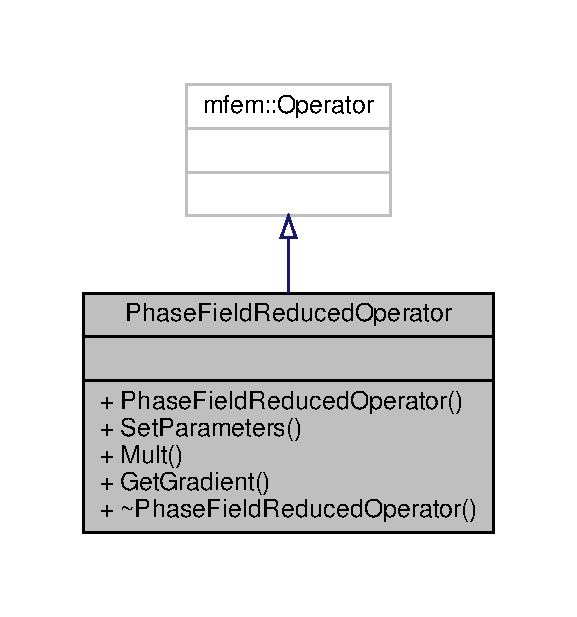
\includegraphics[width=277pt]{classPhaseFieldReducedOperator__inherit__graph}
\end{center}
\end{figure}


Collaboration diagram for Phase\+Field\+Reduced\+Operator\+:\nopagebreak
\begin{figure}[H]
\begin{center}
\leavevmode
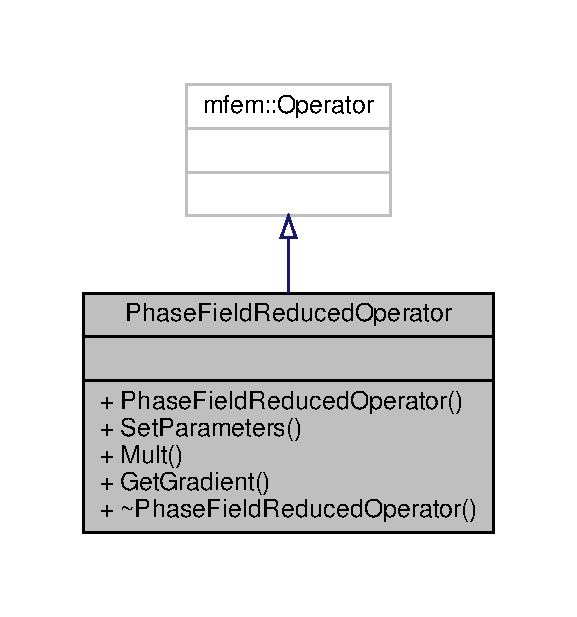
\includegraphics[width=277pt]{classPhaseFieldReducedOperator__coll__graph}
\end{center}
\end{figure}
\subsection*{Public Member Functions}
\begin{DoxyCompactItemize}
\item 
\mbox{\Hypertarget{classPhaseFieldReducedOperator_a4e7966ec91d7c60a60933d9379bbc9bb}\label{classPhaseFieldReducedOperator_a4e7966ec91d7c60a60933d9379bbc9bb}} 
{\bfseries Phase\+Field\+Reduced\+Operator} (mfem\+::\+Bilinear\+Form $\ast$M\+\_\+, mfem\+::\+Nonlinear\+Form $\ast$N\+\_\+)
\item 
\mbox{\Hypertarget{classPhaseFieldReducedOperator_aaaa55d33260a9dc98051bd97f916bf46}\label{classPhaseFieldReducedOperator_aaaa55d33260a9dc98051bd97f916bf46}} 
void \hyperlink{classPhaseFieldReducedOperator_aaaa55d33260a9dc98051bd97f916bf46}{Set\+Parameters} (double dt\+\_\+, const mfem\+::\+Vector $\ast$unk\+\_\+)
\begin{DoxyCompactList}\small\item\em Set current dt, unk values -\/ needed to compute action and Jacobian. \end{DoxyCompactList}\item 
\mbox{\Hypertarget{classPhaseFieldReducedOperator_a3ca66ba9df28451a8648e00db03222e1}\label{classPhaseFieldReducedOperator_a3ca66ba9df28451a8648e00db03222e1}} 
void \hyperlink{classPhaseFieldReducedOperator_a3ca66ba9df28451a8648e00db03222e1}{Mult} (const mfem\+::\+Vector \&k, mfem\+::\+Vector \&y) const
\begin{DoxyCompactList}\small\item\em Compute y = N(unk + dt$\ast$k) + M k. \end{DoxyCompactList}\item 
\mbox{\Hypertarget{classPhaseFieldReducedOperator_aa52eaf1e61d9713732e23eb891ad9b05}\label{classPhaseFieldReducedOperator_aa52eaf1e61d9713732e23eb891ad9b05}} 
mfem\+::\+Operator \& \hyperlink{classPhaseFieldReducedOperator_aa52eaf1e61d9713732e23eb891ad9b05}{Get\+Gradient} (const mfem\+::\+Vector \&k) const
\begin{DoxyCompactList}\small\item\em Compute y = dt$\ast$grad\+\_\+N(unk + dt$\ast$k) + M. \end{DoxyCompactList}\end{DoxyCompactItemize}


\subsection{Detailed Description}


Definition at line 22 of file Reduced\+Operator.\+hpp.



The documentation for this class was generated from the following file\+:\begin{DoxyCompactItemize}
\item 
Reduced\+Operator.\+hpp\end{DoxyCompactItemize}

\hypertarget{classPostProcessing}{}\section{Post\+Processing$<$ T, DC, D\+IM $>$ Class Template Reference}
\label{classPostProcessing}\index{Post\+Processing$<$ T, D\+C, D\+I\+M $>$@{Post\+Processing$<$ T, D\+C, D\+I\+M $>$}}


Inheritance diagram for Post\+Processing$<$ T, DC, D\+IM $>$\+:\nopagebreak
\begin{figure}[H]
\begin{center}
\leavevmode
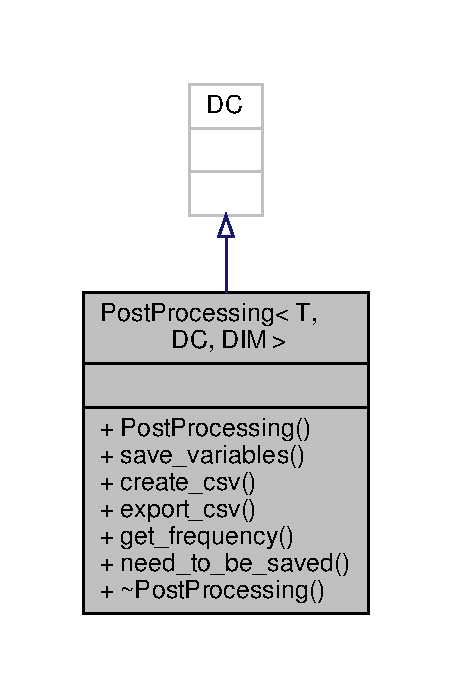
\includegraphics[width=217pt]{classPostProcessing__inherit__graph}
\end{center}
\end{figure}


Collaboration diagram for Post\+Processing$<$ T, DC, D\+IM $>$\+:\nopagebreak
\begin{figure}[H]
\begin{center}
\leavevmode
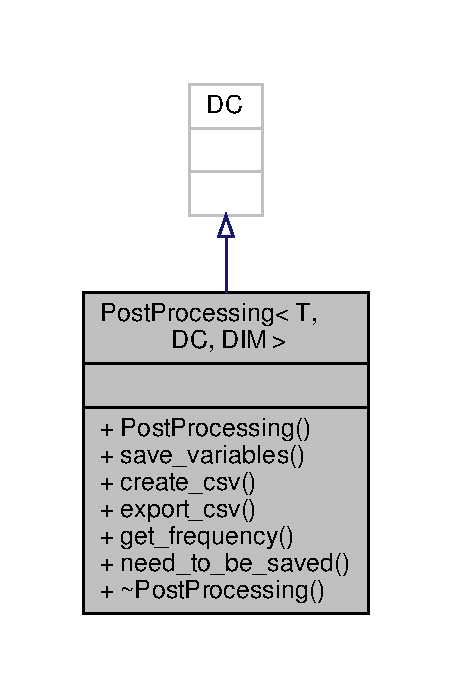
\includegraphics[width=217pt]{classPostProcessing__coll__graph}
\end{center}
\end{figure}
\subsection*{Public Member Functions}
\begin{DoxyCompactItemize}
\item 
\hyperlink{classPostProcessing_a1a7d26c5723dd72ed8fc84eb9e6c6d96}{Post\+Processing} (const std\+::string \&main\+\_\+folder\+\_\+path, const std\+::string \&calculation\+\_\+path, \hyperlink{classSpatialDiscretization}{Spatial\+Discretization}$<$ T, D\+IM $>$ $\ast$space, const int \&frequency, const int \&level\+\_\+of\+\_\+detail)
\begin{DoxyCompactList}\small\item\em Construct a new Post Processing\+:\+: Post Processing object. \end{DoxyCompactList}\item 
void \hyperlink{classPostProcessing_a5872fc7f3527be648339ec33e9536578}{save\+\_\+variables} (const \hyperlink{classVariables}{Variables}$<$ T, D\+IM $>$ \&vars, const int \&iter, const double \&time)
\begin{DoxyCompactList}\small\item\em save variables objet at given iter/time \end{DoxyCompactList}\item 
void \hyperlink{classPostProcessing_a01429a9b4b583e48cd9c4125fb5e85a7}{create\+\_\+csv} (const std\+::string \&filename, const std\+::string \&headers)
\begin{DoxyCompactList}\small\item\em create csv file from name, overwrite if already exist \end{DoxyCompactList}\item 
void \hyperlink{classPostProcessing_a0a7dab69d6e8871063ff9851393b7f86}{export\+\_\+csv} (const std\+::string \&filename, const std\+::map$<$ std\+::tuple$<$ int, double, double $>$, double $>$ \&map\+\_\+results)
\begin{DoxyCompactList}\small\item\em export results into C\+SV file \end{DoxyCompactList}\item 
int \hyperlink{classPostProcessing_a910c85495a35f8e3303c17ece732fdcd}{get\+\_\+frequency} ()
\begin{DoxyCompactList}\small\item\em Get the frequency of post-\/processing in terms of number of iterations (1 means each iteration) \end{DoxyCompactList}\item 
bool \hyperlink{classPostProcessing_ad8a8e567536f9ac9a891d86abe202efe}{need\+\_\+to\+\_\+be\+\_\+saved} (const int \&iteration)
\begin{DoxyCompactList}\small\item\em check if results have to be saved at iteration \end{DoxyCompactList}\item 
\mbox{\Hypertarget{classPostProcessing_abe60f0da8bdd9d606e546dee22114f3c}\label{classPostProcessing_abe60f0da8bdd9d606e546dee22114f3c}} 
\hyperlink{classPostProcessing_abe60f0da8bdd9d606e546dee22114f3c}{$\sim$\+Post\+Processing} ()
\begin{DoxyCompactList}\small\item\em Destroy the Post Processing\+:\+: Post Processing object. \end{DoxyCompactList}\end{DoxyCompactItemize}


\subsection{Detailed Description}
\subsubsection*{template$<$class T, class DC, int D\+IM$>$\newline
class Post\+Processing$<$ T, D\+C, D\+I\+M $>$}



Definition at line 26 of file postprocessing.\+hpp.



\subsection{Constructor \& Destructor Documentation}
\mbox{\Hypertarget{classPostProcessing_a1a7d26c5723dd72ed8fc84eb9e6c6d96}\label{classPostProcessing_a1a7d26c5723dd72ed8fc84eb9e6c6d96}} 
\index{Post\+Processing@{Post\+Processing}!Post\+Processing@{Post\+Processing}}
\index{Post\+Processing@{Post\+Processing}!Post\+Processing@{Post\+Processing}}
\subsubsection{\texorpdfstring{Post\+Processing()}{PostProcessing()}}
{\footnotesize\ttfamily template$<$class T , class DC , int D\+IM$>$ \\
\hyperlink{classPostProcessing}{Post\+Processing}$<$ T, DC, D\+IM $>$\+::\hyperlink{classPostProcessing}{Post\+Processing} (\begin{DoxyParamCaption}\item[{const std\+::string \&}]{main\+\_\+folder\+\_\+path,  }\item[{const std\+::string \&}]{calculation\+\_\+path,  }\item[{\hyperlink{classSpatialDiscretization}{Spatial\+Discretization}$<$ T, D\+IM $>$ $\ast$}]{space,  }\item[{const int \&}]{frequency,  }\item[{const int \&}]{level\+\_\+of\+\_\+detail }\end{DoxyParamCaption})}



Construct a new Post Processing\+:\+: Post Processing object. 


\begin{DoxyParams}{Parameters}
{\em main\+\_\+folder\+\_\+path} & \\
\hline
{\em calculation\+\_\+path} & \\
\hline
{\em mesh} & \\
\hline
{\em level\+\_\+of\+\_\+detail} & \\
\hline
\end{DoxyParams}


Definition at line 56 of file postprocessing.\+hpp.


\begin{DoxyCode}
60     : DC(calculation\_path, &space->\hyperlink{classSpatialDiscretization_ae83ff765cb60c2805cd2f4c00e85b6b2}{get\_mesh}()), frequency\_(frequency) \{
61   this->SetPrefixPath(main\_folder\_path);
62   this->SetLevelsOfDetail(level\_of\_detail);
63   this->SetDataFormat(mfem::VTKFormat::BINARY);
64   this->SetHighOrderOutput(\textcolor{keyword}{true});
65 \}
\end{DoxyCode}


\subsection{Member Function Documentation}
\mbox{\Hypertarget{classPostProcessing_a01429a9b4b583e48cd9c4125fb5e85a7}\label{classPostProcessing_a01429a9b4b583e48cd9c4125fb5e85a7}} 
\index{Post\+Processing@{Post\+Processing}!create\+\_\+csv@{create\+\_\+csv}}
\index{create\+\_\+csv@{create\+\_\+csv}!Post\+Processing@{Post\+Processing}}
\subsubsection{\texorpdfstring{create\+\_\+csv()}{create\_csv()}}
{\footnotesize\ttfamily template$<$class T , class DC , int D\+IM$>$ \\
void \hyperlink{classPostProcessing}{Post\+Processing}$<$ T, DC, D\+IM $>$\+::create\+\_\+csv (\begin{DoxyParamCaption}\item[{const std\+::string \&}]{filename,  }\item[{const std\+::string \&}]{headers }\end{DoxyParamCaption})}



create csv file from name, overwrite if already exist 


\begin{DoxyTemplParams}{Template Parameters}
{\em T} & \\
\hline
{\em DC} & \\
\hline
{\em D\+IM} & \\
\hline
\end{DoxyTemplParams}

\begin{DoxyParams}{Parameters}
{\em filename} & \\
\hline
\end{DoxyParams}


Definition at line 95 of file postprocessing.\+hpp.


\begin{DoxyCode}
96                                                                       \{
97   std::ios\_base::openmode mode = std::ios::out | std::ios::trunc;
98   std::ofstream fic;
99   fic.open(filename, mode);
100   fic << headers;
101   fic << std::endl;
102   fic.close();
103 \}
\end{DoxyCode}
\mbox{\Hypertarget{classPostProcessing_a0a7dab69d6e8871063ff9851393b7f86}\label{classPostProcessing_a0a7dab69d6e8871063ff9851393b7f86}} 
\index{Post\+Processing@{Post\+Processing}!export\+\_\+csv@{export\+\_\+csv}}
\index{export\+\_\+csv@{export\+\_\+csv}!Post\+Processing@{Post\+Processing}}
\subsubsection{\texorpdfstring{export\+\_\+csv()}{export\_csv()}}
{\footnotesize\ttfamily template$<$class T , class DC , int D\+IM$>$ \\
void \hyperlink{classPostProcessing}{Post\+Processing}$<$ T, DC, D\+IM $>$\+::export\+\_\+csv (\begin{DoxyParamCaption}\item[{const std\+::string \&}]{filename,  }\item[{const std\+::map$<$ std\+::tuple$<$ int, double, double $>$, double $>$ \&}]{map\+\_\+results }\end{DoxyParamCaption})}



export results into C\+SV file 


\begin{DoxyTemplParams}{Template Parameters}
{\em T} & \\
\hline
{\em DC} & \\
\hline
{\em D\+IM} & \\
\hline
\end{DoxyTemplParams}

\begin{DoxyParams}{Parameters}
{\em map\+\_\+results} & \\
\hline
\end{DoxyParams}


Definition at line 114 of file postprocessing.\+hpp.


\begin{DoxyCode}
116                                                                       \{
117   std::ios\_base::openmode mode = std::ios::out | std::ios::app;
118   std::ofstream fic;
119   fic.open(filename, mode);
120   std::ostringstream text2fic;
121   \textcolor{comment}{// TODO(CCI) : template + forward ?}
122   \textcolor{keywordflow}{for} (\textcolor{keyword}{auto} [key, value] : map\_results) \{
123     text2fic << std::get<0>(key) << \textcolor{stringliteral}{" "} << std::get<1>(key) << \textcolor{stringliteral}{" "} << std::get<2>(key) << \textcolor{stringliteral}{" "}
124              << value << \textcolor{stringliteral}{"\(\backslash\)n"};
125   \}
126   fic << text2fic.str();
127   fic.close();
128 \}
\end{DoxyCode}
\mbox{\Hypertarget{classPostProcessing_a910c85495a35f8e3303c17ece732fdcd}\label{classPostProcessing_a910c85495a35f8e3303c17ece732fdcd}} 
\index{Post\+Processing@{Post\+Processing}!get\+\_\+frequency@{get\+\_\+frequency}}
\index{get\+\_\+frequency@{get\+\_\+frequency}!Post\+Processing@{Post\+Processing}}
\subsubsection{\texorpdfstring{get\+\_\+frequency()}{get\_frequency()}}
{\footnotesize\ttfamily template$<$class T , class DC , int D\+IM$>$ \\
int \hyperlink{classPostProcessing}{Post\+Processing}$<$ T, DC, D\+IM $>$\+::get\+\_\+frequency (\begin{DoxyParamCaption}{ }\end{DoxyParamCaption})}



Get the frequency of post-\/processing in terms of number of iterations (1 means each iteration) 

\begin{DoxyReturn}{Returns}
int 
\end{DoxyReturn}


Definition at line 136 of file postprocessing.\+hpp.


\begin{DoxyCode}
136                                               \{
137   \textcolor{keywordflow}{return} this->frequency\_;
138 \}
\end{DoxyCode}
\mbox{\Hypertarget{classPostProcessing_ad8a8e567536f9ac9a891d86abe202efe}\label{classPostProcessing_ad8a8e567536f9ac9a891d86abe202efe}} 
\index{Post\+Processing@{Post\+Processing}!need\+\_\+to\+\_\+be\+\_\+saved@{need\+\_\+to\+\_\+be\+\_\+saved}}
\index{need\+\_\+to\+\_\+be\+\_\+saved@{need\+\_\+to\+\_\+be\+\_\+saved}!Post\+Processing@{Post\+Processing}}
\subsubsection{\texorpdfstring{need\+\_\+to\+\_\+be\+\_\+saved()}{need\_to\_be\_saved()}}
{\footnotesize\ttfamily template$<$class T , class DC , int D\+IM$>$ \\
bool \hyperlink{classPostProcessing}{Post\+Processing}$<$ T, DC, D\+IM $>$\+::need\+\_\+to\+\_\+be\+\_\+saved (\begin{DoxyParamCaption}\item[{const int \&}]{iteration }\end{DoxyParamCaption})}



check if results have to be saved at iteration 


\begin{DoxyParams}{Parameters}
{\em iteration} & \\
\hline
\end{DoxyParams}
\begin{DoxyReturn}{Returns}
true 

false 
\end{DoxyReturn}


Definition at line 148 of file postprocessing.\+hpp.


\begin{DoxyCode}
148                                                                       \{
149   \textcolor{keywordtype}{bool} check = (iteration % this->frequency\_ == 0);
150   \textcolor{keywordflow}{return} check;
151 \}
\end{DoxyCode}
\mbox{\Hypertarget{classPostProcessing_a5872fc7f3527be648339ec33e9536578}\label{classPostProcessing_a5872fc7f3527be648339ec33e9536578}} 
\index{Post\+Processing@{Post\+Processing}!save\+\_\+variables@{save\+\_\+variables}}
\index{save\+\_\+variables@{save\+\_\+variables}!Post\+Processing@{Post\+Processing}}
\subsubsection{\texorpdfstring{save\+\_\+variables()}{save\_variables()}}
{\footnotesize\ttfamily template$<$class T , class DC , int D\+IM$>$ \\
void \hyperlink{classPostProcessing}{Post\+Processing}$<$ T, DC, D\+IM $>$\+::save\+\_\+variables (\begin{DoxyParamCaption}\item[{const \hyperlink{classVariables}{Variables}$<$ T, D\+IM $>$ \&}]{vars,  }\item[{const int \&}]{iter,  }\item[{const double \&}]{time }\end{DoxyParamCaption})}



save variables objet at given iter/time 


\begin{DoxyParams}{Parameters}
{\em vars} & \\
\hline
{\em iter} & \\
\hline
{\em time} & \\
\hline
\end{DoxyParams}


Definition at line 75 of file postprocessing.\+hpp.



References Variables$<$ T, D\+I\+M $>$\+::get\+\_\+map\+\_\+gridfunction().


\begin{DoxyCode}
76                                                                     \{
77   this->SetCycle(iter);
78   this->SetTime(time);
79   \textcolor{keyword}{auto} map\_var = vars.\hyperlink{classVariables_a7ab9f249a888212662722a2ca0cae69f}{get\_map\_gridfunction}();
80   \textcolor{keywordflow}{for} (\textcolor{keyword}{auto} [name, gf] : map\_var) \{
81     this->RegisterField(name, &gf);
82     this->Save();
83   \}
84 \}
\end{DoxyCode}


The documentation for this class was generated from the following file\+:\begin{DoxyCompactItemize}
\item 
postprocessing.\+hpp\end{DoxyCompactItemize}

\hypertarget{structpotential__function}{}\section{potential\+\_\+function$<$ O\+R\+D\+ER, S\+C\+H\+E\+ME $>$ Struct Template Reference}
\label{structpotential__function}\index{potential\+\_\+function$<$ O\+R\+D\+E\+R, S\+C\+H\+E\+M\+E $>$@{potential\+\_\+function$<$ O\+R\+D\+E\+R, S\+C\+H\+E\+M\+E $>$}}


Collaboration diagram for potential\+\_\+function$<$ O\+R\+D\+ER, S\+C\+H\+E\+ME $>$\+:\nopagebreak
\begin{figure}[H]
\begin{center}
\leavevmode
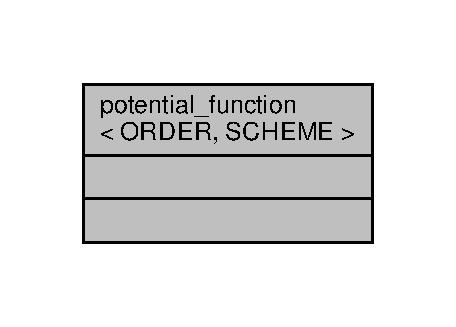
\includegraphics[width=219pt]{structpotential__function__coll__graph}
\end{center}
\end{figure}


\subsection{Detailed Description}
\subsubsection*{template$<$int O\+R\+D\+ER, Thermodynamics\+Potential\+Discretization S\+C\+H\+E\+ME$>$\newline
struct potential\+\_\+function$<$ O\+R\+D\+E\+R, S\+C\+H\+E\+M\+E $>$}



Definition at line 22 of file Phase\+Field\+Potentials.\+hpp.



The documentation for this struct was generated from the following file\+:\begin{DoxyCompactItemize}
\item 
Phase\+Field\+Potentials.\+hpp\end{DoxyCompactItemize}

\hypertarget{structpotential__function_3_010_00_01ThermodynamicsPotentialDiscretization_1_1Explicit_01_4}{}\section{potential\+\_\+function$<$ 0, Thermodynamics\+Potential\+Discretization\+:\+:Explicit $>$ Struct Template Reference}
\label{structpotential__function_3_010_00_01ThermodynamicsPotentialDiscretization_1_1Explicit_01_4}\index{potential\+\_\+function$<$ 0, Thermodynamics\+Potential\+Discretization\+::\+Explicit $>$@{potential\+\_\+function$<$ 0, Thermodynamics\+Potential\+Discretization\+::\+Explicit $>$}}


Collaboration diagram for potential\+\_\+function$<$ 0, Thermodynamics\+Potential\+Discretization\+:\+:Explicit $>$\+:\nopagebreak
\begin{figure}[H]
\begin{center}
\leavevmode
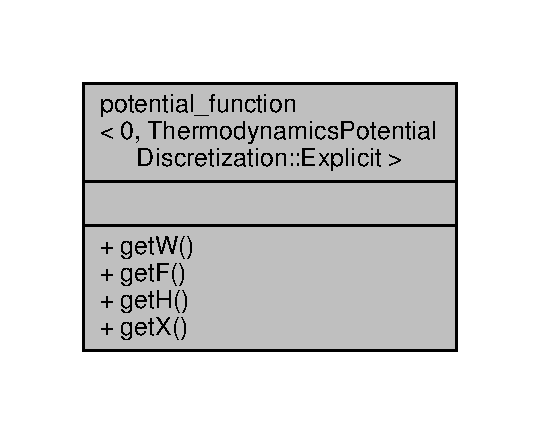
\includegraphics[width=259pt]{structpotential__function_3_010_00_01ThermodynamicsPotentialDiscretization_1_1Explicit_01_4__coll__graph}
\end{center}
\end{figure}
\subsection*{Public Member Functions}
\begin{DoxyCompactItemize}
\item 
{\footnotesize template$<$typename... Args$>$ }\\std\+::function$<$ double(const double \&)$>$ \hyperlink{structpotential__function_3_010_00_01ThermodynamicsPotentialDiscretization_1_1Explicit_01_4_aad1f4c29167d929c6da7b701539a40b0}{getW} (Args... args)
\begin{DoxyCompactList}\small\item\em Double Well potential W(x)=x² $\ast$ (1-\/x)² \end{DoxyCompactList}\item 
{\footnotesize template$<$typename... Args$>$ }\\std\+::function$<$ double(const double \&)$>$ \hyperlink{structpotential__function_3_010_00_01ThermodynamicsPotentialDiscretization_1_1Explicit_01_4_ac2cb58d964d6727a364a8f7a39f57f93}{getF} (Args... args)
\begin{DoxyCompactList}\small\item\em F potential F(x)=(x² -\/1)/4. \end{DoxyCompactList}\item 
{\footnotesize template$<$typename... Args$>$ }\\std\+::function$<$ double(const double \&)$>$ \hyperlink{structpotential__function_3_010_00_01ThermodynamicsPotentialDiscretization_1_1Explicit_01_4_a61efe16deb68d2a92e1e160fc71240b9}{getH} (Args... args)
\begin{DoxyCompactList}\small\item\em Interpolation potential H(x)=x³ $\ast$ (6x²-\/15x+10) \end{DoxyCompactList}\item 
{\footnotesize template$<$typename... Args$>$ }\\std\+::function$<$ double(const double \&)$>$ \hyperlink{structpotential__function_3_010_00_01ThermodynamicsPotentialDiscretization_1_1Explicit_01_4_a47e7aead8ac26c18694091e060c480e9}{getX} (Args... args)
\begin{DoxyCompactList}\small\item\em Identity potential X(x)=x. \end{DoxyCompactList}\end{DoxyCompactItemize}


\subsection{Detailed Description}
\subsubsection*{template$<$$>$\newline
struct potential\+\_\+function$<$ 0, Thermodynamics\+Potential\+Discretization\+::\+Explicit $>$}



Definition at line 257 of file Phase\+Field\+Potentials.\+hpp.



\subsection{Member Function Documentation}
\mbox{\Hypertarget{structpotential__function_3_010_00_01ThermodynamicsPotentialDiscretization_1_1Explicit_01_4_ac2cb58d964d6727a364a8f7a39f57f93}\label{structpotential__function_3_010_00_01ThermodynamicsPotentialDiscretization_1_1Explicit_01_4_ac2cb58d964d6727a364a8f7a39f57f93}} 
\index{potential\+\_\+function$<$ 0, Thermodynamics\+Potential\+Discretization\+::\+Explicit $>$@{potential\+\_\+function$<$ 0, Thermodynamics\+Potential\+Discretization\+::\+Explicit $>$}!getF@{getF}}
\index{getF@{getF}!potential\+\_\+function$<$ 0, Thermodynamics\+Potential\+Discretization\+::\+Explicit $>$@{potential\+\_\+function$<$ 0, Thermodynamics\+Potential\+Discretization\+::\+Explicit $>$}}
\subsubsection{\texorpdfstring{get\+F()}{getF()}}
{\footnotesize\ttfamily template$<$typename... Args$>$ \\
std\+::function$<$double(const double\&)$>$ \hyperlink{structpotential__function}{potential\+\_\+function}$<$ 0, Thermodynamics\+Potential\+Discretization\+::\+Explicit $>$\+::getF (\begin{DoxyParamCaption}\item[{Args...}]{args }\end{DoxyParamCaption})\hspace{0.3cm}{\ttfamily [inline]}}



F potential F(x)=(x² -\/1)/4. 


\begin{DoxyTemplParams}{Template Parameters}
{\em Args} & \\
\hline
\end{DoxyTemplParams}

\begin{DoxyParams}{Parameters}
{\em args} & \\
\hline
\end{DoxyParams}
\begin{DoxyReturn}{Returns}
std\+::function$<$double(const double\&)$>$ 
\end{DoxyReturn}


Definition at line 288 of file Phase\+Field\+Potentials.\+hpp.


\begin{DoxyCode}
288                                                         \{
289     \textcolor{keyword}{auto} v = std::vector<double>\{args...\};
290 
291     \textcolor{keywordflow}{if} (v.size() == 1) \{
292       \textcolor{keyword}{const} \textcolor{keyword}{auto} xn = v[0];
293       \textcolor{keywordflow}{return} std::function<double(const double&)>([xn](\textcolor{keywordtype}{double} x) \{
294         \textcolor{keyword}{const} \textcolor{keyword}{auto} pot = 0.25 * (xn * xn - 1.0) * (xn * xn - 1.0);
295         \textcolor{keywordflow}{return} pot;
296       \});
297     \} \textcolor{keywordflow}{else} \{
298       \textcolor{keywordflow}{throw} std::runtime\_error(
299           \textcolor{stringliteral}{"potential\_function::getF: only one argument is expected for explicit scheme"});
300     \}
301   \}
\end{DoxyCode}
\mbox{\Hypertarget{structpotential__function_3_010_00_01ThermodynamicsPotentialDiscretization_1_1Explicit_01_4_a61efe16deb68d2a92e1e160fc71240b9}\label{structpotential__function_3_010_00_01ThermodynamicsPotentialDiscretization_1_1Explicit_01_4_a61efe16deb68d2a92e1e160fc71240b9}} 
\index{potential\+\_\+function$<$ 0, Thermodynamics\+Potential\+Discretization\+::\+Explicit $>$@{potential\+\_\+function$<$ 0, Thermodynamics\+Potential\+Discretization\+::\+Explicit $>$}!getH@{getH}}
\index{getH@{getH}!potential\+\_\+function$<$ 0, Thermodynamics\+Potential\+Discretization\+::\+Explicit $>$@{potential\+\_\+function$<$ 0, Thermodynamics\+Potential\+Discretization\+::\+Explicit $>$}}
\subsubsection{\texorpdfstring{get\+H()}{getH()}}
{\footnotesize\ttfamily template$<$typename... Args$>$ \\
std\+::function$<$double(const double\&)$>$ \hyperlink{structpotential__function}{potential\+\_\+function}$<$ 0, Thermodynamics\+Potential\+Discretization\+::\+Explicit $>$\+::getH (\begin{DoxyParamCaption}\item[{Args...}]{args }\end{DoxyParamCaption})\hspace{0.3cm}{\ttfamily [inline]}}



Interpolation potential H(x)=x³ $\ast$ (6x²-\/15x+10) 


\begin{DoxyTemplParams}{Template Parameters}
{\em Args} & \\
\hline
\end{DoxyTemplParams}

\begin{DoxyParams}{Parameters}
{\em args} & \\
\hline
\end{DoxyParams}
\begin{DoxyReturn}{Returns}
std\+::function$<$double(const double\&)$>$ 
\end{DoxyReturn}


Definition at line 310 of file Phase\+Field\+Potentials.\+hpp.


\begin{DoxyCode}
310                                                         \{
311     \textcolor{keyword}{auto} v = std::vector<double>\{args...\};
312 
313     \textcolor{keywordflow}{if} (v.size() == 1) \{
314       \textcolor{keyword}{const} \textcolor{keyword}{auto} xn = v[0];
315       \textcolor{keywordflow}{return} std::function<double(const double&)>([xn](\textcolor{keywordtype}{double} x) \{
316         \textcolor{keyword}{const} \textcolor{keyword}{auto} pot = xn * xn * xn * (6.0 * xn * xn - 15.0 * xn + 10.0);
317         \textcolor{keywordflow}{return} pot;
318       \});
319     \} \textcolor{keywordflow}{else} \{
320       \textcolor{keywordflow}{throw} std::runtime\_error(
321           \textcolor{stringliteral}{"potential\_function::getH: only one argument is expected for explicit scheme"});
322     \}
323   \}
\end{DoxyCode}
\mbox{\Hypertarget{structpotential__function_3_010_00_01ThermodynamicsPotentialDiscretization_1_1Explicit_01_4_aad1f4c29167d929c6da7b701539a40b0}\label{structpotential__function_3_010_00_01ThermodynamicsPotentialDiscretization_1_1Explicit_01_4_aad1f4c29167d929c6da7b701539a40b0}} 
\index{potential\+\_\+function$<$ 0, Thermodynamics\+Potential\+Discretization\+::\+Explicit $>$@{potential\+\_\+function$<$ 0, Thermodynamics\+Potential\+Discretization\+::\+Explicit $>$}!getW@{getW}}
\index{getW@{getW}!potential\+\_\+function$<$ 0, Thermodynamics\+Potential\+Discretization\+::\+Explicit $>$@{potential\+\_\+function$<$ 0, Thermodynamics\+Potential\+Discretization\+::\+Explicit $>$}}
\subsubsection{\texorpdfstring{get\+W()}{getW()}}
{\footnotesize\ttfamily template$<$typename... Args$>$ \\
std\+::function$<$double(const double\&)$>$ \hyperlink{structpotential__function}{potential\+\_\+function}$<$ 0, Thermodynamics\+Potential\+Discretization\+::\+Explicit $>$\+::getW (\begin{DoxyParamCaption}\item[{Args...}]{args }\end{DoxyParamCaption})\hspace{0.3cm}{\ttfamily [inline]}}



Double Well potential W(x)=x² $\ast$ (1-\/x)² 


\begin{DoxyTemplParams}{Template Parameters}
{\em Args} & \\
\hline
\end{DoxyTemplParams}

\begin{DoxyParams}{Parameters}
{\em args} & \\
\hline
\end{DoxyParams}
\begin{DoxyReturn}{Returns}
std\+::function$<$double(const double\&)$>$ 
\end{DoxyReturn}


Definition at line 266 of file Phase\+Field\+Potentials.\+hpp.


\begin{DoxyCode}
266                                                         \{
267     \textcolor{keyword}{auto} v = std::vector<double>\{args...\};
268 
269     \textcolor{keywordflow}{if} (v.size() == 1) \{
270       \textcolor{keyword}{const} \textcolor{keyword}{auto} xn = v[0];
271       \textcolor{keywordflow}{return} std::function<double(const double&)>([xn](\textcolor{keywordtype}{double} x) \{
272         \textcolor{keyword}{const} \textcolor{keyword}{auto} pot = xn * xn * (1.0 - xn) * (1.0 - xn);
273         \textcolor{keywordflow}{return} pot;
274       \});
275     \} \textcolor{keywordflow}{else} \{
276       \textcolor{keywordflow}{throw} std::runtime\_error(
277           \textcolor{stringliteral}{"potential\_function::getW: only one argument is expected for explicit scheme"});
278     \}
279   \}
\end{DoxyCode}
\mbox{\Hypertarget{structpotential__function_3_010_00_01ThermodynamicsPotentialDiscretization_1_1Explicit_01_4_a47e7aead8ac26c18694091e060c480e9}\label{structpotential__function_3_010_00_01ThermodynamicsPotentialDiscretization_1_1Explicit_01_4_a47e7aead8ac26c18694091e060c480e9}} 
\index{potential\+\_\+function$<$ 0, Thermodynamics\+Potential\+Discretization\+::\+Explicit $>$@{potential\+\_\+function$<$ 0, Thermodynamics\+Potential\+Discretization\+::\+Explicit $>$}!getX@{getX}}
\index{getX@{getX}!potential\+\_\+function$<$ 0, Thermodynamics\+Potential\+Discretization\+::\+Explicit $>$@{potential\+\_\+function$<$ 0, Thermodynamics\+Potential\+Discretization\+::\+Explicit $>$}}
\subsubsection{\texorpdfstring{get\+X()}{getX()}}
{\footnotesize\ttfamily template$<$typename... Args$>$ \\
std\+::function$<$double(const double\&)$>$ \hyperlink{structpotential__function}{potential\+\_\+function}$<$ 0, Thermodynamics\+Potential\+Discretization\+::\+Explicit $>$\+::getX (\begin{DoxyParamCaption}\item[{Args...}]{args }\end{DoxyParamCaption})\hspace{0.3cm}{\ttfamily [inline]}}



Identity potential X(x)=x. 


\begin{DoxyTemplParams}{Template Parameters}
{\em Args} & \\
\hline
\end{DoxyTemplParams}

\begin{DoxyParams}{Parameters}
{\em args} & \\
\hline
\end{DoxyParams}
\begin{DoxyReturn}{Returns}
std\+::function$<$double(const double\&)$>$ 
\end{DoxyReturn}


Definition at line 332 of file Phase\+Field\+Potentials.\+hpp.


\begin{DoxyCode}
332                                                         \{
333     \textcolor{keyword}{auto} v = std::vector<double>\{args...\};
334 
335     \textcolor{keywordflow}{if} (v.size() == 1) \{
336       \textcolor{keyword}{const} \textcolor{keyword}{auto} xn = v[0];
337       \textcolor{keywordflow}{return} std::function<double(const double&)>([xn](\textcolor{keywordtype}{double} x) \{
338         \textcolor{keyword}{const} \textcolor{keyword}{auto} pot = xn;
339         \textcolor{keywordflow}{return} pot;
340       \});
341     \} \textcolor{keywordflow}{else} \{
342       \textcolor{keywordflow}{throw} std::runtime\_error(
343           \textcolor{stringliteral}{"potential\_function::getX: only one argument is expected for explicit scheme"});
344     \}
345   \}
\end{DoxyCode}


The documentation for this struct was generated from the following file\+:\begin{DoxyCompactItemize}
\item 
Phase\+Field\+Potentials.\+hpp\end{DoxyCompactItemize}

\hypertarget{structpotential__function_3_010_00_01ThermodynamicsPotentialDiscretization_1_1Implicit_01_4}{}\section{potential\+\_\+function$<$ 0, Thermodynamics\+Potential\+Discretization\+:\+:Implicit $>$ Struct Template Reference}
\label{structpotential__function_3_010_00_01ThermodynamicsPotentialDiscretization_1_1Implicit_01_4}\index{potential\+\_\+function$<$ 0, Thermodynamics\+Potential\+Discretization\+::\+Implicit $>$@{potential\+\_\+function$<$ 0, Thermodynamics\+Potential\+Discretization\+::\+Implicit $>$}}


Collaboration diagram for potential\+\_\+function$<$ 0, Thermodynamics\+Potential\+Discretization\+:\+:Implicit $>$\+:\nopagebreak
\begin{figure}[H]
\begin{center}
\leavevmode
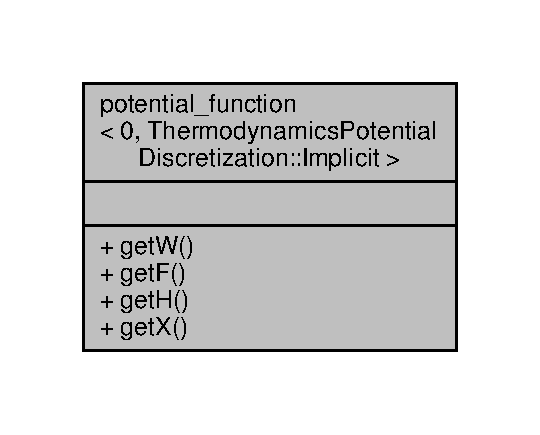
\includegraphics[width=259pt]{structpotential__function_3_010_00_01ThermodynamicsPotentialDiscretization_1_1Implicit_01_4__coll__graph}
\end{center}
\end{figure}
\subsection*{Public Member Functions}
\begin{DoxyCompactItemize}
\item 
{\footnotesize template$<$typename... Args$>$ }\\std\+::function$<$ double(const double \&)$>$ \hyperlink{structpotential__function_3_010_00_01ThermodynamicsPotentialDiscretization_1_1Implicit_01_4_ac15781824e0ce378683ca91749cd6eb8}{getW} (Args... args)
\begin{DoxyCompactList}\small\item\em Double Well potential W(x)=x² $\ast$ (1-\/x)² \end{DoxyCompactList}\item 
{\footnotesize template$<$typename... Args$>$ }\\std\+::function$<$ double(const double \&)$>$ \hyperlink{structpotential__function_3_010_00_01ThermodynamicsPotentialDiscretization_1_1Implicit_01_4_a18b8e58d6110096f4edb09d4d4df53e7}{getF} (Args... args)
\begin{DoxyCompactList}\small\item\em F potential F(x)=(x² -\/1)/4. \end{DoxyCompactList}\item 
{\footnotesize template$<$typename... Args$>$ }\\std\+::function$<$ double(const double \&)$>$ \hyperlink{structpotential__function_3_010_00_01ThermodynamicsPotentialDiscretization_1_1Implicit_01_4_a74d232601bbe797c14897e297134c938}{getH} (Args... args)
\begin{DoxyCompactList}\small\item\em Interpolation potential H(x)=x³ $\ast$ (6x²-\/15x+10) \end{DoxyCompactList}\item 
{\footnotesize template$<$typename... Args$>$ }\\std\+::function$<$ double(const double \&)$>$ \hyperlink{structpotential__function_3_010_00_01ThermodynamicsPotentialDiscretization_1_1Implicit_01_4_ac1e8415ca039946ab75d5da92b956d7f}{getX} (Args... args)
\begin{DoxyCompactList}\small\item\em Identity potential X(x)=x. \end{DoxyCompactList}\end{DoxyCompactItemize}


\subsection{Detailed Description}
\subsubsection*{template$<$$>$\newline
struct potential\+\_\+function$<$ 0, Thermodynamics\+Potential\+Discretization\+::\+Implicit $>$}



Definition at line 68 of file Phase\+Field\+Potentials.\+hpp.



\subsection{Member Function Documentation}
\mbox{\Hypertarget{structpotential__function_3_010_00_01ThermodynamicsPotentialDiscretization_1_1Implicit_01_4_a18b8e58d6110096f4edb09d4d4df53e7}\label{structpotential__function_3_010_00_01ThermodynamicsPotentialDiscretization_1_1Implicit_01_4_a18b8e58d6110096f4edb09d4d4df53e7}} 
\index{potential\+\_\+function$<$ 0, Thermodynamics\+Potential\+Discretization\+::\+Implicit $>$@{potential\+\_\+function$<$ 0, Thermodynamics\+Potential\+Discretization\+::\+Implicit $>$}!getF@{getF}}
\index{getF@{getF}!potential\+\_\+function$<$ 0, Thermodynamics\+Potential\+Discretization\+::\+Implicit $>$@{potential\+\_\+function$<$ 0, Thermodynamics\+Potential\+Discretization\+::\+Implicit $>$}}
\subsubsection{\texorpdfstring{get\+F()}{getF()}}
{\footnotesize\ttfamily template$<$typename... Args$>$ \\
std\+::function$<$double(const double\&)$>$ \hyperlink{structpotential__function}{potential\+\_\+function}$<$ 0, Thermodynamics\+Potential\+Discretization\+::\+Implicit $>$\+::getF (\begin{DoxyParamCaption}\item[{Args...}]{args }\end{DoxyParamCaption})\hspace{0.3cm}{\ttfamily [inline]}}



F potential F(x)=(x² -\/1)/4. 


\begin{DoxyTemplParams}{Template Parameters}
{\em Args} & \\
\hline
\end{DoxyTemplParams}

\begin{DoxyParams}{Parameters}
{\em args} & \\
\hline
\end{DoxyParams}
\begin{DoxyReturn}{Returns}
std\+::function$<$double(const double\&)$>$ 
\end{DoxyReturn}


Definition at line 91 of file Phase\+Field\+Potentials.\+hpp.


\begin{DoxyCode}
91                                                         \{
92     \textcolor{keywordflow}{return} std::function<double(const double&)>([](\textcolor{keywordtype}{double} x) \{
93       \textcolor{keyword}{const} \textcolor{keyword}{auto} pot = 0.25 * (x * x - 1.0) * (x * x - 1.0);
94       \textcolor{keywordflow}{return} pot;
95     \});
96   \}
\end{DoxyCode}
\mbox{\Hypertarget{structpotential__function_3_010_00_01ThermodynamicsPotentialDiscretization_1_1Implicit_01_4_a74d232601bbe797c14897e297134c938}\label{structpotential__function_3_010_00_01ThermodynamicsPotentialDiscretization_1_1Implicit_01_4_a74d232601bbe797c14897e297134c938}} 
\index{potential\+\_\+function$<$ 0, Thermodynamics\+Potential\+Discretization\+::\+Implicit $>$@{potential\+\_\+function$<$ 0, Thermodynamics\+Potential\+Discretization\+::\+Implicit $>$}!getH@{getH}}
\index{getH@{getH}!potential\+\_\+function$<$ 0, Thermodynamics\+Potential\+Discretization\+::\+Implicit $>$@{potential\+\_\+function$<$ 0, Thermodynamics\+Potential\+Discretization\+::\+Implicit $>$}}
\subsubsection{\texorpdfstring{get\+H()}{getH()}}
{\footnotesize\ttfamily template$<$typename... Args$>$ \\
std\+::function$<$double(const double\&)$>$ \hyperlink{structpotential__function}{potential\+\_\+function}$<$ 0, Thermodynamics\+Potential\+Discretization\+::\+Implicit $>$\+::getH (\begin{DoxyParamCaption}\item[{Args...}]{args }\end{DoxyParamCaption})\hspace{0.3cm}{\ttfamily [inline]}}



Interpolation potential H(x)=x³ $\ast$ (6x²-\/15x+10) 


\begin{DoxyTemplParams}{Template Parameters}
{\em Args} & \\
\hline
\end{DoxyTemplParams}

\begin{DoxyParams}{Parameters}
{\em args} & \\
\hline
\end{DoxyParams}
\begin{DoxyReturn}{Returns}
std\+::function$<$double(const double\&)$>$ 
\end{DoxyReturn}


Definition at line 105 of file Phase\+Field\+Potentials.\+hpp.


\begin{DoxyCode}
105                                                         \{
106     \textcolor{keywordflow}{return} std::function<double(const double&)>([](\textcolor{keywordtype}{double} x) \{
107       \textcolor{keyword}{const} \textcolor{keyword}{auto} pot = x * x * x * (6.0 * x * x - 15.0 * x + 10.0);
108       \textcolor{keywordflow}{return} pot;
109     \});
110   \}
\end{DoxyCode}
\mbox{\Hypertarget{structpotential__function_3_010_00_01ThermodynamicsPotentialDiscretization_1_1Implicit_01_4_ac15781824e0ce378683ca91749cd6eb8}\label{structpotential__function_3_010_00_01ThermodynamicsPotentialDiscretization_1_1Implicit_01_4_ac15781824e0ce378683ca91749cd6eb8}} 
\index{potential\+\_\+function$<$ 0, Thermodynamics\+Potential\+Discretization\+::\+Implicit $>$@{potential\+\_\+function$<$ 0, Thermodynamics\+Potential\+Discretization\+::\+Implicit $>$}!getW@{getW}}
\index{getW@{getW}!potential\+\_\+function$<$ 0, Thermodynamics\+Potential\+Discretization\+::\+Implicit $>$@{potential\+\_\+function$<$ 0, Thermodynamics\+Potential\+Discretization\+::\+Implicit $>$}}
\subsubsection{\texorpdfstring{get\+W()}{getW()}}
{\footnotesize\ttfamily template$<$typename... Args$>$ \\
std\+::function$<$double(const double\&)$>$ \hyperlink{structpotential__function}{potential\+\_\+function}$<$ 0, Thermodynamics\+Potential\+Discretization\+::\+Implicit $>$\+::getW (\begin{DoxyParamCaption}\item[{Args...}]{args }\end{DoxyParamCaption})\hspace{0.3cm}{\ttfamily [inline]}}



Double Well potential W(x)=x² $\ast$ (1-\/x)² 


\begin{DoxyTemplParams}{Template Parameters}
{\em Args} & \\
\hline
\end{DoxyTemplParams}

\begin{DoxyParams}{Parameters}
{\em args} & \\
\hline
\end{DoxyParams}
\begin{DoxyReturn}{Returns}
std\+::function$<$double(const double\&)$>$ 
\end{DoxyReturn}


Definition at line 77 of file Phase\+Field\+Potentials.\+hpp.


\begin{DoxyCode}
77                                                         \{
78     \textcolor{keywordflow}{return} std::function<double(const double&)>([](\textcolor{keywordtype}{double} x) \{
79       \textcolor{keyword}{const} \textcolor{keyword}{auto} pot = x * x * (1.0 - x) * (1.0 - x);
80       \textcolor{keywordflow}{return} pot;
81     \});
82   \}
\end{DoxyCode}
\mbox{\Hypertarget{structpotential__function_3_010_00_01ThermodynamicsPotentialDiscretization_1_1Implicit_01_4_ac1e8415ca039946ab75d5da92b956d7f}\label{structpotential__function_3_010_00_01ThermodynamicsPotentialDiscretization_1_1Implicit_01_4_ac1e8415ca039946ab75d5da92b956d7f}} 
\index{potential\+\_\+function$<$ 0, Thermodynamics\+Potential\+Discretization\+::\+Implicit $>$@{potential\+\_\+function$<$ 0, Thermodynamics\+Potential\+Discretization\+::\+Implicit $>$}!getX@{getX}}
\index{getX@{getX}!potential\+\_\+function$<$ 0, Thermodynamics\+Potential\+Discretization\+::\+Implicit $>$@{potential\+\_\+function$<$ 0, Thermodynamics\+Potential\+Discretization\+::\+Implicit $>$}}
\subsubsection{\texorpdfstring{get\+X()}{getX()}}
{\footnotesize\ttfamily template$<$typename... Args$>$ \\
std\+::function$<$double(const double\&)$>$ \hyperlink{structpotential__function}{potential\+\_\+function}$<$ 0, Thermodynamics\+Potential\+Discretization\+::\+Implicit $>$\+::getX (\begin{DoxyParamCaption}\item[{Args...}]{args }\end{DoxyParamCaption})\hspace{0.3cm}{\ttfamily [inline]}}



Identity potential X(x)=x. 


\begin{DoxyTemplParams}{Template Parameters}
{\em Args} & \\
\hline
\end{DoxyTemplParams}

\begin{DoxyParams}{Parameters}
{\em args} & \\
\hline
\end{DoxyParams}
\begin{DoxyReturn}{Returns}
std\+::function$<$double(const double\&)$>$ 
\end{DoxyReturn}


Definition at line 119 of file Phase\+Field\+Potentials.\+hpp.


\begin{DoxyCode}
119                                                         \{
120     \textcolor{keywordflow}{return} std::function<double(const double&)>([](\textcolor{keywordtype}{double} x) \{
121       \textcolor{keyword}{const} \textcolor{keyword}{auto} pot = x;
122       \textcolor{keywordflow}{return} pot;
123     \});
124   \}
\end{DoxyCode}


The documentation for this struct was generated from the following file\+:\begin{DoxyCompactItemize}
\item 
Phase\+Field\+Potentials.\+hpp\end{DoxyCompactItemize}

\hypertarget{structpotential__function_3_010_00_01ThermodynamicsPotentialDiscretization_1_1SemiImplicit_01_4}{}\section{potential\+\_\+function$<$ 0, Thermodynamics\+Potential\+Discretization\+:\+:Semi\+Implicit $>$ Struct Template Reference}
\label{structpotential__function_3_010_00_01ThermodynamicsPotentialDiscretization_1_1SemiImplicit_01_4}\index{potential\+\_\+function$<$ 0, Thermodynamics\+Potential\+Discretization\+::\+Semi\+Implicit $>$@{potential\+\_\+function$<$ 0, Thermodynamics\+Potential\+Discretization\+::\+Semi\+Implicit $>$}}


Collaboration diagram for potential\+\_\+function$<$ 0, Thermodynamics\+Potential\+Discretization\+:\+:Semi\+Implicit $>$\+:\nopagebreak
\begin{figure}[H]
\begin{center}
\leavevmode
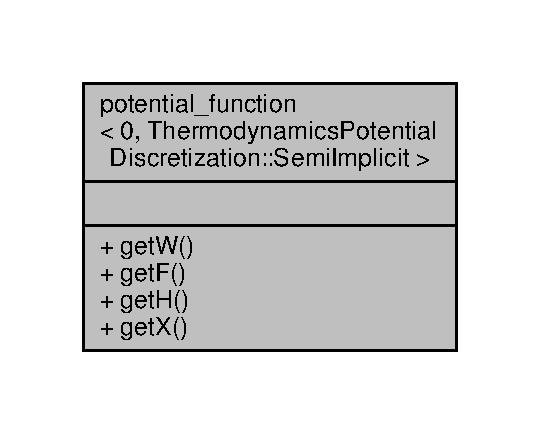
\includegraphics[width=259pt]{structpotential__function_3_010_00_01ThermodynamicsPotentialDiscretization_1_1SemiImplicit_01_4__coll__graph}
\end{center}
\end{figure}
\subsection*{Public Member Functions}
\begin{DoxyCompactItemize}
\item 
{\footnotesize template$<$typename... Args$>$ }\\std\+::function$<$ double(const double \&)$>$ \hyperlink{structpotential__function_3_010_00_01ThermodynamicsPotentialDiscretization_1_1SemiImplicit_01_4_afb01c48fefb8549b46f1df57dee9e19e}{getW} (Args... args)
\begin{DoxyCompactList}\small\item\em Double Well potential W(x)=x² $\ast$ (1-\/x)² with semi-\/implicit scheme (as implicit/explicit schemes) \end{DoxyCompactList}\item 
{\footnotesize template$<$typename... Args$>$ }\\std\+::function$<$ double(const double \&)$>$ \hyperlink{structpotential__function_3_010_00_01ThermodynamicsPotentialDiscretization_1_1SemiImplicit_01_4_a9bb69d00c5351b45d864fb056650cd1f}{getF} (Args... args)
\begin{DoxyCompactList}\small\item\em F potential F(x)=(x² -\/1)/4. \end{DoxyCompactList}\item 
{\footnotesize template$<$typename... Args$>$ }\\std\+::function$<$ double(const double \&)$>$ \hyperlink{structpotential__function_3_010_00_01ThermodynamicsPotentialDiscretization_1_1SemiImplicit_01_4_a04b03e529ffbac36d76a9dcd1353c61e}{getH} (Args... args)
\begin{DoxyCompactList}\small\item\em Interpolation potential H(x)=x³ $\ast$ (6x²-\/15x+10) with semi-\/implicit scheme (as implicit/explicit schemes) \end{DoxyCompactList}\item 
{\footnotesize template$<$typename... Args$>$ }\\std\+::function$<$ double(const double \&)$>$ \hyperlink{structpotential__function_3_010_00_01ThermodynamicsPotentialDiscretization_1_1SemiImplicit_01_4_a9c2d3c673cbe8c37d3e9c46820a7ea78}{getX} (Args... args)
\begin{DoxyCompactList}\small\item\em Identity potential X(x)=x with semi-\/implicit scheme (as implicit/explicit schemes) \end{DoxyCompactList}\end{DoxyCompactItemize}


\subsection{Detailed Description}
\subsubsection*{template$<$$>$\newline
struct potential\+\_\+function$<$ 0, Thermodynamics\+Potential\+Discretization\+::\+Semi\+Implicit $>$}



Definition at line 509 of file Phase\+Field\+Potentials.\+hpp.



\subsection{Member Function Documentation}
\mbox{\Hypertarget{structpotential__function_3_010_00_01ThermodynamicsPotentialDiscretization_1_1SemiImplicit_01_4_a9bb69d00c5351b45d864fb056650cd1f}\label{structpotential__function_3_010_00_01ThermodynamicsPotentialDiscretization_1_1SemiImplicit_01_4_a9bb69d00c5351b45d864fb056650cd1f}} 
\index{potential\+\_\+function$<$ 0, Thermodynamics\+Potential\+Discretization\+::\+Semi\+Implicit $>$@{potential\+\_\+function$<$ 0, Thermodynamics\+Potential\+Discretization\+::\+Semi\+Implicit $>$}!getF@{getF}}
\index{getF@{getF}!potential\+\_\+function$<$ 0, Thermodynamics\+Potential\+Discretization\+::\+Semi\+Implicit $>$@{potential\+\_\+function$<$ 0, Thermodynamics\+Potential\+Discretization\+::\+Semi\+Implicit $>$}}
\subsubsection{\texorpdfstring{get\+F()}{getF()}}
{\footnotesize\ttfamily template$<$typename... Args$>$ \\
std\+::function$<$double(const double\&)$>$ \hyperlink{structpotential__function}{potential\+\_\+function}$<$ 0, Thermodynamics\+Potential\+Discretization\+::\+Semi\+Implicit $>$\+::getF (\begin{DoxyParamCaption}\item[{Args...}]{args }\end{DoxyParamCaption})\hspace{0.3cm}{\ttfamily [inline]}}



F potential F(x)=(x² -\/1)/4. 


\begin{DoxyTemplParams}{Template Parameters}
{\em Args} & \\
\hline
\end{DoxyTemplParams}

\begin{DoxyParams}{Parameters}
{\em args} & \\
\hline
\end{DoxyParams}
\begin{DoxyReturn}{Returns}
std\+::function$<$double(const double\&)$>$ 
\end{DoxyReturn}


Definition at line 533 of file Phase\+Field\+Potentials.\+hpp.


\begin{DoxyCode}
533                                                         \{
534     \textcolor{keywordflow}{return} std::function<double(const double&)>([](\textcolor{keywordtype}{double} x) \{
535       \textcolor{keyword}{const} \textcolor{keyword}{auto} pot = 0.25 * (x * x - 1.0) * (x * x - 1.0);
536       \textcolor{keywordflow}{return} pot;
537     \});
538   \}
\end{DoxyCode}
\mbox{\Hypertarget{structpotential__function_3_010_00_01ThermodynamicsPotentialDiscretization_1_1SemiImplicit_01_4_a04b03e529ffbac36d76a9dcd1353c61e}\label{structpotential__function_3_010_00_01ThermodynamicsPotentialDiscretization_1_1SemiImplicit_01_4_a04b03e529ffbac36d76a9dcd1353c61e}} 
\index{potential\+\_\+function$<$ 0, Thermodynamics\+Potential\+Discretization\+::\+Semi\+Implicit $>$@{potential\+\_\+function$<$ 0, Thermodynamics\+Potential\+Discretization\+::\+Semi\+Implicit $>$}!getH@{getH}}
\index{getH@{getH}!potential\+\_\+function$<$ 0, Thermodynamics\+Potential\+Discretization\+::\+Semi\+Implicit $>$@{potential\+\_\+function$<$ 0, Thermodynamics\+Potential\+Discretization\+::\+Semi\+Implicit $>$}}
\subsubsection{\texorpdfstring{get\+H()}{getH()}}
{\footnotesize\ttfamily template$<$typename... Args$>$ \\
std\+::function$<$double(const double\&)$>$ \hyperlink{structpotential__function}{potential\+\_\+function}$<$ 0, Thermodynamics\+Potential\+Discretization\+::\+Semi\+Implicit $>$\+::getH (\begin{DoxyParamCaption}\item[{Args...}]{args }\end{DoxyParamCaption})\hspace{0.3cm}{\ttfamily [inline]}}



Interpolation potential H(x)=x³ $\ast$ (6x²-\/15x+10) with semi-\/implicit scheme (as implicit/explicit schemes) 


\begin{DoxyTemplParams}{Template Parameters}
{\em Args} & \\
\hline
\end{DoxyTemplParams}

\begin{DoxyParams}{Parameters}
{\em args} & \\
\hline
\end{DoxyParams}
\begin{DoxyReturn}{Returns}
std\+::function$<$double(const double\&)$>$ 
\end{DoxyReturn}


Definition at line 548 of file Phase\+Field\+Potentials.\+hpp.


\begin{DoxyCode}
548                                                         \{
549     \textcolor{keywordflow}{return} std::function<double(const double&)>([](\textcolor{keywordtype}{double} x) \{
550       \textcolor{keyword}{const} \textcolor{keyword}{auto} pot = x * x * x * (6.0 * x * x - 15.0 * x + 10.0);
551       \textcolor{keywordflow}{return} pot;
552     \});
553   \}
\end{DoxyCode}
\mbox{\Hypertarget{structpotential__function_3_010_00_01ThermodynamicsPotentialDiscretization_1_1SemiImplicit_01_4_afb01c48fefb8549b46f1df57dee9e19e}\label{structpotential__function_3_010_00_01ThermodynamicsPotentialDiscretization_1_1SemiImplicit_01_4_afb01c48fefb8549b46f1df57dee9e19e}} 
\index{potential\+\_\+function$<$ 0, Thermodynamics\+Potential\+Discretization\+::\+Semi\+Implicit $>$@{potential\+\_\+function$<$ 0, Thermodynamics\+Potential\+Discretization\+::\+Semi\+Implicit $>$}!getW@{getW}}
\index{getW@{getW}!potential\+\_\+function$<$ 0, Thermodynamics\+Potential\+Discretization\+::\+Semi\+Implicit $>$@{potential\+\_\+function$<$ 0, Thermodynamics\+Potential\+Discretization\+::\+Semi\+Implicit $>$}}
\subsubsection{\texorpdfstring{get\+W()}{getW()}}
{\footnotesize\ttfamily template$<$typename... Args$>$ \\
std\+::function$<$double(const double\&)$>$ \hyperlink{structpotential__function}{potential\+\_\+function}$<$ 0, Thermodynamics\+Potential\+Discretization\+::\+Semi\+Implicit $>$\+::getW (\begin{DoxyParamCaption}\item[{Args...}]{args }\end{DoxyParamCaption})\hspace{0.3cm}{\ttfamily [inline]}}



Double Well potential W(x)=x² $\ast$ (1-\/x)² with semi-\/implicit scheme (as implicit/explicit schemes) 


\begin{DoxyTemplParams}{Template Parameters}
{\em Args} & \\
\hline
\end{DoxyTemplParams}

\begin{DoxyParams}{Parameters}
{\em args} & \\
\hline
\end{DoxyParams}
\begin{DoxyReturn}{Returns}
std\+::function$<$double(const double\&)$>$ 
\end{DoxyReturn}


Definition at line 519 of file Phase\+Field\+Potentials.\+hpp.


\begin{DoxyCode}
519                                                         \{
520     \textcolor{keywordflow}{return} std::function<double(const double&)>([](\textcolor{keywordtype}{double} x) \{
521       \textcolor{keyword}{const} \textcolor{keyword}{auto} pot = x * x * (1.0 - x) * (1.0 - x);
522       \textcolor{keywordflow}{return} pot;
523     \});
524   \}
\end{DoxyCode}
\mbox{\Hypertarget{structpotential__function_3_010_00_01ThermodynamicsPotentialDiscretization_1_1SemiImplicit_01_4_a9c2d3c673cbe8c37d3e9c46820a7ea78}\label{structpotential__function_3_010_00_01ThermodynamicsPotentialDiscretization_1_1SemiImplicit_01_4_a9c2d3c673cbe8c37d3e9c46820a7ea78}} 
\index{potential\+\_\+function$<$ 0, Thermodynamics\+Potential\+Discretization\+::\+Semi\+Implicit $>$@{potential\+\_\+function$<$ 0, Thermodynamics\+Potential\+Discretization\+::\+Semi\+Implicit $>$}!getX@{getX}}
\index{getX@{getX}!potential\+\_\+function$<$ 0, Thermodynamics\+Potential\+Discretization\+::\+Semi\+Implicit $>$@{potential\+\_\+function$<$ 0, Thermodynamics\+Potential\+Discretization\+::\+Semi\+Implicit $>$}}
\subsubsection{\texorpdfstring{get\+X()}{getX()}}
{\footnotesize\ttfamily template$<$typename... Args$>$ \\
std\+::function$<$double(const double\&)$>$ \hyperlink{structpotential__function}{potential\+\_\+function}$<$ 0, Thermodynamics\+Potential\+Discretization\+::\+Semi\+Implicit $>$\+::getX (\begin{DoxyParamCaption}\item[{Args...}]{args }\end{DoxyParamCaption})\hspace{0.3cm}{\ttfamily [inline]}}



Identity potential X(x)=x with semi-\/implicit scheme (as implicit/explicit schemes) 


\begin{DoxyTemplParams}{Template Parameters}
{\em Args} & \\
\hline
\end{DoxyTemplParams}

\begin{DoxyParams}{Parameters}
{\em args} & \\
\hline
\end{DoxyParams}
\begin{DoxyReturn}{Returns}
std\+::function$<$double(const double\&)$>$ 
\end{DoxyReturn}


Definition at line 563 of file Phase\+Field\+Potentials.\+hpp.


\begin{DoxyCode}
563                                                         \{
564     \textcolor{keywordflow}{return} std::function<double(const double&)>([](\textcolor{keywordtype}{double} x) \{
565       \textcolor{keyword}{const} \textcolor{keyword}{auto} pot = x;
566       \textcolor{keywordflow}{return} pot;
567     \});
568   \}
\end{DoxyCode}


The documentation for this struct was generated from the following file\+:\begin{DoxyCompactItemize}
\item 
Phase\+Field\+Potentials.\+hpp\end{DoxyCompactItemize}

\hypertarget{structpotential__function_3_011_00_01ThermodynamicsPotentialDiscretization_1_1Explicit_01_4}{}\section{potential\+\_\+function$<$ 1, Thermodynamics\+Potential\+Discretization\+:\+:Explicit $>$ Struct Template Reference}
\label{structpotential__function_3_011_00_01ThermodynamicsPotentialDiscretization_1_1Explicit_01_4}\index{potential\+\_\+function$<$ 1, Thermodynamics\+Potential\+Discretization\+::\+Explicit $>$@{potential\+\_\+function$<$ 1, Thermodynamics\+Potential\+Discretization\+::\+Explicit $>$}}


Collaboration diagram for potential\+\_\+function$<$ 1, Thermodynamics\+Potential\+Discretization\+:\+:Explicit $>$\+:\nopagebreak
\begin{figure}[H]
\begin{center}
\leavevmode
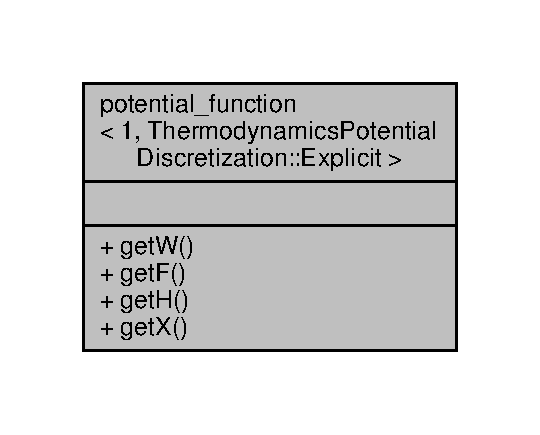
\includegraphics[width=259pt]{structpotential__function_3_011_00_01ThermodynamicsPotentialDiscretization_1_1Explicit_01_4__coll__graph}
\end{center}
\end{figure}
\subsection*{Public Member Functions}
\begin{DoxyCompactItemize}
\item 
{\footnotesize template$<$typename... Args$>$ }\\std\+::function$<$ double(const double \&)$>$ \hyperlink{structpotential__function_3_011_00_01ThermodynamicsPotentialDiscretization_1_1Explicit_01_4_a83b90abf5c35bfe033a38d32ad812db1}{getW} (Args... args)
\begin{DoxyCompactList}\small\item\em First derivative of the double Well potential W(x)=x² $\ast$ (1-\/x)² with explicit scheme (as implicit scheme) \end{DoxyCompactList}\item 
{\footnotesize template$<$typename... Args$>$ }\\std\+::function$<$ double(const double \&)$>$ \hyperlink{structpotential__function_3_011_00_01ThermodynamicsPotentialDiscretization_1_1Explicit_01_4_aa5b8fb0d4c1b1bc1661eff409466133a}{getF} (Args... args)
\begin{DoxyCompactList}\small\item\em First derivative of the F potential F(x)=(x² -\/1)/4. \end{DoxyCompactList}\item 
{\footnotesize template$<$typename... Args$>$ }\\std\+::function$<$ double(const double \&)$>$ \hyperlink{structpotential__function_3_011_00_01ThermodynamicsPotentialDiscretization_1_1Explicit_01_4_a7b08d20c38b06d405bc33d028ba6bad0}{getH} (Args... args)
\begin{DoxyCompactList}\small\item\em First derivative of the interpolation potential H(x)=x³ $\ast$ (6x²-\/15x+10) with explicit scheme (as implicit scheme) \end{DoxyCompactList}\item 
{\footnotesize template$<$typename... Args$>$ }\\std\+::function$<$ double(const double \&)$>$ \hyperlink{structpotential__function_3_011_00_01ThermodynamicsPotentialDiscretization_1_1Explicit_01_4_aaf5a701d015b3c450af251a86a2e66c2}{getX} (Args... args)
\begin{DoxyCompactList}\small\item\em First derivative of the identity potential X(x)=x with explicit scheme (as implicit scheme) \end{DoxyCompactList}\end{DoxyCompactItemize}


\subsection{Detailed Description}
\subsubsection*{template$<$$>$\newline
struct potential\+\_\+function$<$ 1, Thermodynamics\+Potential\+Discretization\+::\+Explicit $>$}



Definition at line 351 of file Phase\+Field\+Potentials.\+hpp.



\subsection{Member Function Documentation}
\mbox{\Hypertarget{structpotential__function_3_011_00_01ThermodynamicsPotentialDiscretization_1_1Explicit_01_4_aa5b8fb0d4c1b1bc1661eff409466133a}\label{structpotential__function_3_011_00_01ThermodynamicsPotentialDiscretization_1_1Explicit_01_4_aa5b8fb0d4c1b1bc1661eff409466133a}} 
\index{potential\+\_\+function$<$ 1, Thermodynamics\+Potential\+Discretization\+::\+Explicit $>$@{potential\+\_\+function$<$ 1, Thermodynamics\+Potential\+Discretization\+::\+Explicit $>$}!getF@{getF}}
\index{getF@{getF}!potential\+\_\+function$<$ 1, Thermodynamics\+Potential\+Discretization\+::\+Explicit $>$@{potential\+\_\+function$<$ 1, Thermodynamics\+Potential\+Discretization\+::\+Explicit $>$}}
\subsubsection{\texorpdfstring{get\+F()}{getF()}}
{\footnotesize\ttfamily template$<$typename... Args$>$ \\
std\+::function$<$double(const double\&)$>$ \hyperlink{structpotential__function}{potential\+\_\+function}$<$ 1, Thermodynamics\+Potential\+Discretization\+::\+Explicit $>$\+::getF (\begin{DoxyParamCaption}\item[{Args...}]{args }\end{DoxyParamCaption})\hspace{0.3cm}{\ttfamily [inline]}}



First derivative of the F potential F(x)=(x² -\/1)/4. 


\begin{DoxyTemplParams}{Template Parameters}
{\em Args} & \\
\hline
\end{DoxyTemplParams}

\begin{DoxyParams}{Parameters}
{\em args} & \\
\hline
\end{DoxyParams}
\begin{DoxyReturn}{Returns}
std\+::function$<$double(const double\&)$>$ 
\end{DoxyReturn}


Definition at line 384 of file Phase\+Field\+Potentials.\+hpp.


\begin{DoxyCode}
384                                                         \{
385     \textcolor{keyword}{auto} v = std::vector<double>\{args...\};
386 
387     \textcolor{keywordflow}{if} (v.size() == 1) \{
388       \textcolor{keyword}{const} \textcolor{keyword}{auto} xn = v[0];
389       \textcolor{keywordflow}{return} std::function<double(const double&)>([xn](\textcolor{keywordtype}{double} x) \{
390         \textcolor{keyword}{const} \textcolor{keyword}{auto} pot = xn * (xn * xn - 1.0);
391         \textcolor{keywordflow}{return} pot;
392       \});
393     \} \textcolor{keywordflow}{else} \{
394       \textcolor{keywordflow}{throw} std::runtime\_error(
395           \textcolor{stringliteral}{"potential\_function::getF: only one argument is expected for explicit scheme"});
396     \}
397   \}
\end{DoxyCode}
\mbox{\Hypertarget{structpotential__function_3_011_00_01ThermodynamicsPotentialDiscretization_1_1Explicit_01_4_a7b08d20c38b06d405bc33d028ba6bad0}\label{structpotential__function_3_011_00_01ThermodynamicsPotentialDiscretization_1_1Explicit_01_4_a7b08d20c38b06d405bc33d028ba6bad0}} 
\index{potential\+\_\+function$<$ 1, Thermodynamics\+Potential\+Discretization\+::\+Explicit $>$@{potential\+\_\+function$<$ 1, Thermodynamics\+Potential\+Discretization\+::\+Explicit $>$}!getH@{getH}}
\index{getH@{getH}!potential\+\_\+function$<$ 1, Thermodynamics\+Potential\+Discretization\+::\+Explicit $>$@{potential\+\_\+function$<$ 1, Thermodynamics\+Potential\+Discretization\+::\+Explicit $>$}}
\subsubsection{\texorpdfstring{get\+H()}{getH()}}
{\footnotesize\ttfamily template$<$typename... Args$>$ \\
std\+::function$<$double(const double\&)$>$ \hyperlink{structpotential__function}{potential\+\_\+function}$<$ 1, Thermodynamics\+Potential\+Discretization\+::\+Explicit $>$\+::getH (\begin{DoxyParamCaption}\item[{Args...}]{args }\end{DoxyParamCaption})\hspace{0.3cm}{\ttfamily [inline]}}



First derivative of the interpolation potential H(x)=x³ $\ast$ (6x²-\/15x+10) with explicit scheme (as implicit scheme) 


\begin{DoxyTemplParams}{Template Parameters}
{\em Args} & \\
\hline
\end{DoxyTemplParams}

\begin{DoxyParams}{Parameters}
{\em args} & \\
\hline
\end{DoxyParams}
\begin{DoxyReturn}{Returns}
std\+::function$<$double(const double\&)$>$ 
\end{DoxyReturn}


Definition at line 407 of file Phase\+Field\+Potentials.\+hpp.


\begin{DoxyCode}
407                                                         \{
408     \textcolor{keyword}{auto} v = std::vector<double>\{args...\};
409 
410     \textcolor{keywordflow}{if} (v.size() == 1) \{
411       \textcolor{keyword}{const} \textcolor{keyword}{auto} xn = v[0];
412       \textcolor{keywordflow}{return} std::function<double(const double&)>([xn](\textcolor{keywordtype}{double} x) \{
413         \textcolor{keyword}{const} \textcolor{keyword}{auto} pot = 30. * xn * xn * (1.0 - xn) * (1.0 - xn);
414         \textcolor{keywordflow}{return} pot;
415       \});
416     \} \textcolor{keywordflow}{else} \{
417       \textcolor{keywordflow}{throw} std::runtime\_error(
418           \textcolor{stringliteral}{"potential\_function::getH: only one argument is expected for explicit scheme"});
419     \}
420   \}
\end{DoxyCode}
\mbox{\Hypertarget{structpotential__function_3_011_00_01ThermodynamicsPotentialDiscretization_1_1Explicit_01_4_a83b90abf5c35bfe033a38d32ad812db1}\label{structpotential__function_3_011_00_01ThermodynamicsPotentialDiscretization_1_1Explicit_01_4_a83b90abf5c35bfe033a38d32ad812db1}} 
\index{potential\+\_\+function$<$ 1, Thermodynamics\+Potential\+Discretization\+::\+Explicit $>$@{potential\+\_\+function$<$ 1, Thermodynamics\+Potential\+Discretization\+::\+Explicit $>$}!getW@{getW}}
\index{getW@{getW}!potential\+\_\+function$<$ 1, Thermodynamics\+Potential\+Discretization\+::\+Explicit $>$@{potential\+\_\+function$<$ 1, Thermodynamics\+Potential\+Discretization\+::\+Explicit $>$}}
\subsubsection{\texorpdfstring{get\+W()}{getW()}}
{\footnotesize\ttfamily template$<$typename... Args$>$ \\
std\+::function$<$double(const double\&)$>$ \hyperlink{structpotential__function}{potential\+\_\+function}$<$ 1, Thermodynamics\+Potential\+Discretization\+::\+Explicit $>$\+::getW (\begin{DoxyParamCaption}\item[{Args...}]{args }\end{DoxyParamCaption})\hspace{0.3cm}{\ttfamily [inline]}}



First derivative of the double Well potential W(x)=x² $\ast$ (1-\/x)² with explicit scheme (as implicit scheme) 


\begin{DoxyTemplParams}{Template Parameters}
{\em Args} & \\
\hline
\end{DoxyTemplParams}

\begin{DoxyParams}{Parameters}
{\em args} & \\
\hline
\end{DoxyParams}
\begin{DoxyReturn}{Returns}
std\+::function$<$double(const double\&)$>$ 
\end{DoxyReturn}


Definition at line 361 of file Phase\+Field\+Potentials.\+hpp.


\begin{DoxyCode}
361                                                         \{
362     \textcolor{keyword}{auto} v = std::vector<double>\{args...\};
363 
364     \textcolor{keywordflow}{if} (v.size() == 1) \{
365       \textcolor{keyword}{const} \textcolor{keyword}{auto} xn = v[0];
366       \textcolor{keywordflow}{return} std::function<double(const double&)>([xn](\textcolor{keywordtype}{double} x) \{
367         \textcolor{keyword}{const} \textcolor{keyword}{auto} pot = 2. * xn * (1.0 - xn) * (1.0 - 2. * xn);
368         \textcolor{keywordflow}{return} pot;
369       \});
370     \} \textcolor{keywordflow}{else} \{
371       \textcolor{keywordflow}{throw} std::runtime\_error(
372           \textcolor{stringliteral}{"potential\_function::getW: only one argument is expected for explicit scheme"});
373     \}
374   \}
\end{DoxyCode}
\mbox{\Hypertarget{structpotential__function_3_011_00_01ThermodynamicsPotentialDiscretization_1_1Explicit_01_4_aaf5a701d015b3c450af251a86a2e66c2}\label{structpotential__function_3_011_00_01ThermodynamicsPotentialDiscretization_1_1Explicit_01_4_aaf5a701d015b3c450af251a86a2e66c2}} 
\index{potential\+\_\+function$<$ 1, Thermodynamics\+Potential\+Discretization\+::\+Explicit $>$@{potential\+\_\+function$<$ 1, Thermodynamics\+Potential\+Discretization\+::\+Explicit $>$}!getX@{getX}}
\index{getX@{getX}!potential\+\_\+function$<$ 1, Thermodynamics\+Potential\+Discretization\+::\+Explicit $>$@{potential\+\_\+function$<$ 1, Thermodynamics\+Potential\+Discretization\+::\+Explicit $>$}}
\subsubsection{\texorpdfstring{get\+X()}{getX()}}
{\footnotesize\ttfamily template$<$typename... Args$>$ \\
std\+::function$<$double(const double\&)$>$ \hyperlink{structpotential__function}{potential\+\_\+function}$<$ 1, Thermodynamics\+Potential\+Discretization\+::\+Explicit $>$\+::getX (\begin{DoxyParamCaption}\item[{Args...}]{args }\end{DoxyParamCaption})\hspace{0.3cm}{\ttfamily [inline]}}



First derivative of the identity potential X(x)=x with explicit scheme (as implicit scheme) 


\begin{DoxyTemplParams}{Template Parameters}
{\em Args} & \\
\hline
\end{DoxyTemplParams}

\begin{DoxyParams}{Parameters}
{\em args} & \\
\hline
\end{DoxyParams}
\begin{DoxyReturn}{Returns}
std\+::function$<$double(const double\&)$>$ 
\end{DoxyReturn}


Definition at line 430 of file Phase\+Field\+Potentials.\+hpp.


\begin{DoxyCode}
430                                                         \{
431     \textcolor{keywordflow}{return} std::function<double(const double&)>([](\textcolor{keywordtype}{double} x) \{
432       \textcolor{keyword}{const} \textcolor{keyword}{auto} pot = 1.;
433       \textcolor{keywordflow}{return} pot;
434     \});
435   \}
\end{DoxyCode}


The documentation for this struct was generated from the following file\+:\begin{DoxyCompactItemize}
\item 
Phase\+Field\+Potentials.\+hpp\end{DoxyCompactItemize}

\hypertarget{structpotential__function_3_011_00_01ThermodynamicsPotentialDiscretization_1_1Implicit_01_4}{}\section{potential\+\_\+function$<$ 1, Thermodynamics\+Potential\+Discretization\+:\+:Implicit $>$ Struct Template Reference}
\label{structpotential__function_3_011_00_01ThermodynamicsPotentialDiscretization_1_1Implicit_01_4}\index{potential\+\_\+function$<$ 1, Thermodynamics\+Potential\+Discretization\+::\+Implicit $>$@{potential\+\_\+function$<$ 1, Thermodynamics\+Potential\+Discretization\+::\+Implicit $>$}}


Collaboration diagram for potential\+\_\+function$<$ 1, Thermodynamics\+Potential\+Discretization\+:\+:Implicit $>$\+:\nopagebreak
\begin{figure}[H]
\begin{center}
\leavevmode
\includegraphics[width=259pt]{structpotential__function_3_011_00_01ThermodynamicsPotentialDiscretization_1_1Implicit_01_4__coll__graph}
\end{center}
\end{figure}
\subsection*{Public Member Functions}
\begin{DoxyCompactItemize}
\item 
{\footnotesize template$<$typename... Args$>$ }\\std\+::function$<$ double(const double \&)$>$ \hyperlink{structpotential__function_3_011_00_01ThermodynamicsPotentialDiscretization_1_1Implicit_01_4_a54faef5e6e6e4acf56b5e473c765532a}{getW} (Args... args)
\begin{DoxyCompactList}\small\item\em First derivative of the double Well potential W(x)=x² $\ast$ (1-\/x)² \end{DoxyCompactList}\item 
{\footnotesize template$<$typename... Args$>$ }\\std\+::function$<$ double(const double \&)$>$ \hyperlink{structpotential__function_3_011_00_01ThermodynamicsPotentialDiscretization_1_1Implicit_01_4_af57f36f2f98b7c524a03273504fa82a7}{getF} (Args... args)
\begin{DoxyCompactList}\small\item\em First derivative of the F potential F(x)=(x² -\/1)/4. \end{DoxyCompactList}\item 
{\footnotesize template$<$typename... Args$>$ }\\std\+::function$<$ double(const double \&)$>$ \hyperlink{structpotential__function_3_011_00_01ThermodynamicsPotentialDiscretization_1_1Implicit_01_4_a6a52cc510f4213371c7e99e4b6fbe477}{getH} (Args... args)
\begin{DoxyCompactList}\small\item\em First derivative of the interpolation potential H(x)=x³ $\ast$ (6x²-\/15x+10) \end{DoxyCompactList}\item 
{\footnotesize template$<$typename... Args$>$ }\\std\+::function$<$ double(const double \&)$>$ \hyperlink{structpotential__function_3_011_00_01ThermodynamicsPotentialDiscretization_1_1Implicit_01_4_ac886230109344fb32f98f4e5816665c7}{getX} (Args... args)
\begin{DoxyCompactList}\small\item\em First derivative of the identity potential X(x)=x. \end{DoxyCompactList}\end{DoxyCompactItemize}


\subsection{Detailed Description}
\subsubsection*{template$<$$>$\newline
struct potential\+\_\+function$<$ 1, Thermodynamics\+Potential\+Discretization\+::\+Implicit $>$}



Definition at line 130 of file Phase\+Field\+Potentials.\+hpp.



\subsection{Member Function Documentation}
\mbox{\Hypertarget{structpotential__function_3_011_00_01ThermodynamicsPotentialDiscretization_1_1Implicit_01_4_af57f36f2f98b7c524a03273504fa82a7}\label{structpotential__function_3_011_00_01ThermodynamicsPotentialDiscretization_1_1Implicit_01_4_af57f36f2f98b7c524a03273504fa82a7}} 
\index{potential\+\_\+function$<$ 1, Thermodynamics\+Potential\+Discretization\+::\+Implicit $>$@{potential\+\_\+function$<$ 1, Thermodynamics\+Potential\+Discretization\+::\+Implicit $>$}!getF@{getF}}
\index{getF@{getF}!potential\+\_\+function$<$ 1, Thermodynamics\+Potential\+Discretization\+::\+Implicit $>$@{potential\+\_\+function$<$ 1, Thermodynamics\+Potential\+Discretization\+::\+Implicit $>$}}
\subsubsection{\texorpdfstring{get\+F()}{getF()}}
{\footnotesize\ttfamily template$<$typename... Args$>$ \\
std\+::function$<$double(const double\&)$>$ \hyperlink{structpotential__function}{potential\+\_\+function}$<$ 1, Thermodynamics\+Potential\+Discretization\+::\+Implicit $>$\+::getF (\begin{DoxyParamCaption}\item[{Args...}]{args }\end{DoxyParamCaption})\hspace{0.3cm}{\ttfamily [inline]}}



First derivative of the F potential F(x)=(x² -\/1)/4. 


\begin{DoxyTemplParams}{Template Parameters}
{\em Args} & \\
\hline
\end{DoxyTemplParams}

\begin{DoxyParams}{Parameters}
{\em args} & \\
\hline
\end{DoxyParams}
\begin{DoxyReturn}{Returns}
std\+::function$<$double(const double\&)$>$ 
\end{DoxyReturn}


Definition at line 153 of file Phase\+Field\+Potentials.\+hpp.


\begin{DoxyCode}
153                                                         \{
154     \textcolor{keywordflow}{return} std::function<double(const double&)>([](\textcolor{keywordtype}{double} x) \{
155       \textcolor{keyword}{const} \textcolor{keyword}{auto} pot = x * x * x - x;
156       \textcolor{keywordflow}{return} pot;
157     \});
158   \}
\end{DoxyCode}
\mbox{\Hypertarget{structpotential__function_3_011_00_01ThermodynamicsPotentialDiscretization_1_1Implicit_01_4_a6a52cc510f4213371c7e99e4b6fbe477}\label{structpotential__function_3_011_00_01ThermodynamicsPotentialDiscretization_1_1Implicit_01_4_a6a52cc510f4213371c7e99e4b6fbe477}} 
\index{potential\+\_\+function$<$ 1, Thermodynamics\+Potential\+Discretization\+::\+Implicit $>$@{potential\+\_\+function$<$ 1, Thermodynamics\+Potential\+Discretization\+::\+Implicit $>$}!getH@{getH}}
\index{getH@{getH}!potential\+\_\+function$<$ 1, Thermodynamics\+Potential\+Discretization\+::\+Implicit $>$@{potential\+\_\+function$<$ 1, Thermodynamics\+Potential\+Discretization\+::\+Implicit $>$}}
\subsubsection{\texorpdfstring{get\+H()}{getH()}}
{\footnotesize\ttfamily template$<$typename... Args$>$ \\
std\+::function$<$double(const double\&)$>$ \hyperlink{structpotential__function}{potential\+\_\+function}$<$ 1, Thermodynamics\+Potential\+Discretization\+::\+Implicit $>$\+::getH (\begin{DoxyParamCaption}\item[{Args...}]{args }\end{DoxyParamCaption})\hspace{0.3cm}{\ttfamily [inline]}}



First derivative of the interpolation potential H(x)=x³ $\ast$ (6x²-\/15x+10) 


\begin{DoxyTemplParams}{Template Parameters}
{\em Args} & \\
\hline
\end{DoxyTemplParams}

\begin{DoxyParams}{Parameters}
{\em args} & \\
\hline
\end{DoxyParams}
\begin{DoxyReturn}{Returns}
std\+::function$<$double(const double\&)$>$ 
\end{DoxyReturn}


Definition at line 167 of file Phase\+Field\+Potentials.\+hpp.


\begin{DoxyCode}
167                                                         \{
168     \textcolor{keywordflow}{return} std::function<double(const double&)>([](\textcolor{keywordtype}{double} x) \{
169       \textcolor{keyword}{const} \textcolor{keyword}{auto} pot = 30. * x * x * (1.0 - x) * (1.0 - x);
170       \textcolor{keywordflow}{return} pot;
171     \});
172   \}
\end{DoxyCode}
\mbox{\Hypertarget{structpotential__function_3_011_00_01ThermodynamicsPotentialDiscretization_1_1Implicit_01_4_a54faef5e6e6e4acf56b5e473c765532a}\label{structpotential__function_3_011_00_01ThermodynamicsPotentialDiscretization_1_1Implicit_01_4_a54faef5e6e6e4acf56b5e473c765532a}} 
\index{potential\+\_\+function$<$ 1, Thermodynamics\+Potential\+Discretization\+::\+Implicit $>$@{potential\+\_\+function$<$ 1, Thermodynamics\+Potential\+Discretization\+::\+Implicit $>$}!getW@{getW}}
\index{getW@{getW}!potential\+\_\+function$<$ 1, Thermodynamics\+Potential\+Discretization\+::\+Implicit $>$@{potential\+\_\+function$<$ 1, Thermodynamics\+Potential\+Discretization\+::\+Implicit $>$}}
\subsubsection{\texorpdfstring{get\+W()}{getW()}}
{\footnotesize\ttfamily template$<$typename... Args$>$ \\
std\+::function$<$double(const double\&)$>$ \hyperlink{structpotential__function}{potential\+\_\+function}$<$ 1, Thermodynamics\+Potential\+Discretization\+::\+Implicit $>$\+::getW (\begin{DoxyParamCaption}\item[{Args...}]{args }\end{DoxyParamCaption})\hspace{0.3cm}{\ttfamily [inline]}}



First derivative of the double Well potential W(x)=x² $\ast$ (1-\/x)² 


\begin{DoxyTemplParams}{Template Parameters}
{\em Args} & \\
\hline
\end{DoxyTemplParams}

\begin{DoxyParams}{Parameters}
{\em args} & \\
\hline
\end{DoxyParams}
\begin{DoxyReturn}{Returns}
std\+::function$<$double(const double\&)$>$ 
\end{DoxyReturn}


Definition at line 139 of file Phase\+Field\+Potentials.\+hpp.


\begin{DoxyCode}
139                                                         \{
140     \textcolor{keywordflow}{return} std::function<double(const double&)>([](\textcolor{keywordtype}{double} x) \{
141       \textcolor{keyword}{const} \textcolor{keyword}{auto} pot = 2. * x * (1.0 - x) * (1.0 - 2. * x);
142       \textcolor{keywordflow}{return} pot;
143     \});
144   \}
\end{DoxyCode}
\mbox{\Hypertarget{structpotential__function_3_011_00_01ThermodynamicsPotentialDiscretization_1_1Implicit_01_4_ac886230109344fb32f98f4e5816665c7}\label{structpotential__function_3_011_00_01ThermodynamicsPotentialDiscretization_1_1Implicit_01_4_ac886230109344fb32f98f4e5816665c7}} 
\index{potential\+\_\+function$<$ 1, Thermodynamics\+Potential\+Discretization\+::\+Implicit $>$@{potential\+\_\+function$<$ 1, Thermodynamics\+Potential\+Discretization\+::\+Implicit $>$}!getX@{getX}}
\index{getX@{getX}!potential\+\_\+function$<$ 1, Thermodynamics\+Potential\+Discretization\+::\+Implicit $>$@{potential\+\_\+function$<$ 1, Thermodynamics\+Potential\+Discretization\+::\+Implicit $>$}}
\subsubsection{\texorpdfstring{get\+X()}{getX()}}
{\footnotesize\ttfamily template$<$typename... Args$>$ \\
std\+::function$<$double(const double\&)$>$ \hyperlink{structpotential__function}{potential\+\_\+function}$<$ 1, Thermodynamics\+Potential\+Discretization\+::\+Implicit $>$\+::getX (\begin{DoxyParamCaption}\item[{Args...}]{args }\end{DoxyParamCaption})\hspace{0.3cm}{\ttfamily [inline]}}



First derivative of the identity potential X(x)=x. 


\begin{DoxyTemplParams}{Template Parameters}
{\em Args} & \\
\hline
\end{DoxyTemplParams}

\begin{DoxyParams}{Parameters}
{\em args} & \\
\hline
\end{DoxyParams}
\begin{DoxyReturn}{Returns}
std\+::function$<$double(const double\&)$>$ 
\end{DoxyReturn}


Definition at line 181 of file Phase\+Field\+Potentials.\+hpp.


\begin{DoxyCode}
181                                                         \{
182     \textcolor{keywordflow}{return} std::function<double(const double&)>([](\textcolor{keywordtype}{double} x) \{
183       \textcolor{keyword}{const} \textcolor{keyword}{auto} pot = 1.;
184       \textcolor{keywordflow}{return} pot;
185     \});
186   \}
\end{DoxyCode}


The documentation for this struct was generated from the following file\+:\begin{DoxyCompactItemize}
\item 
Phase\+Field\+Potentials.\+hpp\end{DoxyCompactItemize}

\hypertarget{structpotential__function_3_011_00_01ThermodynamicsPotentialDiscretization_1_1SemiImplicit_01_4}{}\section{potential\+\_\+function$<$ 1, Thermodynamics\+Potential\+Discretization\+:\+:Semi\+Implicit $>$ Struct Template Reference}
\label{structpotential__function_3_011_00_01ThermodynamicsPotentialDiscretization_1_1SemiImplicit_01_4}\index{potential\+\_\+function$<$ 1, Thermodynamics\+Potential\+Discretization\+::\+Semi\+Implicit $>$@{potential\+\_\+function$<$ 1, Thermodynamics\+Potential\+Discretization\+::\+Semi\+Implicit $>$}}


Collaboration diagram for potential\+\_\+function$<$ 1, Thermodynamics\+Potential\+Discretization\+:\+:Semi\+Implicit $>$\+:\nopagebreak
\begin{figure}[H]
\begin{center}
\leavevmode
\includegraphics[width=259pt]{structpotential__function_3_011_00_01ThermodynamicsPotentialDiscretization_1_1SemiImplicit_01_4__coll__graph}
\end{center}
\end{figure}
\subsection*{Public Member Functions}
\begin{DoxyCompactItemize}
\item 
{\footnotesize template$<$typename... Args$>$ }\\std\+::function$<$ double(const double \&)$>$ \hyperlink{structpotential__function_3_011_00_01ThermodynamicsPotentialDiscretization_1_1SemiImplicit_01_4_af7269239087bb065b4133b36fcbd6da6}{getW} (Args... args)
\begin{DoxyCompactList}\small\item\em First derivative of the double Well potential W(x)=x² $\ast$ (1-\/x)² with semi-\/implicit scheme. \end{DoxyCompactList}\item 
{\footnotesize template$<$typename... Args$>$ }\\std\+::function$<$ double(const double \&)$>$ \hyperlink{structpotential__function_3_011_00_01ThermodynamicsPotentialDiscretization_1_1SemiImplicit_01_4_a27140a669c8f1c66c03bb48bda4f33ff}{getF} (Args... args)
\begin{DoxyCompactList}\small\item\em First derivative of the F potential F(x)=(x² -\/1)/4. \end{DoxyCompactList}\item 
{\footnotesize template$<$typename... Args$>$ }\\std\+::function$<$ double(const double \&)$>$ \hyperlink{structpotential__function_3_011_00_01ThermodynamicsPotentialDiscretization_1_1SemiImplicit_01_4_a82e4c4bf76347666f6e4f394581ee2b3}{getH} (Args... args)
\begin{DoxyCompactList}\small\item\em First derivative of the interpolation potential H(x)=x³ $\ast$ (6x²-\/15x+10) with semi-\/implicit scheme (as implicit/explicit schemes) \end{DoxyCompactList}\item 
{\footnotesize template$<$typename... Args$>$ }\\std\+::function$<$ double(const double \&)$>$ \hyperlink{structpotential__function_3_011_00_01ThermodynamicsPotentialDiscretization_1_1SemiImplicit_01_4_ad139574d08b145db4f8ed0274e0d388e}{getX} (Args... args)
\begin{DoxyCompactList}\small\item\em First derivative of the identity potential X(x)=x with semi-\/implicit scheme (as implicit/explicit schemes) \end{DoxyCompactList}\end{DoxyCompactItemize}


\subsection{Detailed Description}
\subsubsection*{template$<$$>$\newline
struct potential\+\_\+function$<$ 1, Thermodynamics\+Potential\+Discretization\+::\+Semi\+Implicit $>$}



Definition at line 574 of file Phase\+Field\+Potentials.\+hpp.



\subsection{Member Function Documentation}
\mbox{\Hypertarget{structpotential__function_3_011_00_01ThermodynamicsPotentialDiscretization_1_1SemiImplicit_01_4_a27140a669c8f1c66c03bb48bda4f33ff}\label{structpotential__function_3_011_00_01ThermodynamicsPotentialDiscretization_1_1SemiImplicit_01_4_a27140a669c8f1c66c03bb48bda4f33ff}} 
\index{potential\+\_\+function$<$ 1, Thermodynamics\+Potential\+Discretization\+::\+Semi\+Implicit $>$@{potential\+\_\+function$<$ 1, Thermodynamics\+Potential\+Discretization\+::\+Semi\+Implicit $>$}!getF@{getF}}
\index{getF@{getF}!potential\+\_\+function$<$ 1, Thermodynamics\+Potential\+Discretization\+::\+Semi\+Implicit $>$@{potential\+\_\+function$<$ 1, Thermodynamics\+Potential\+Discretization\+::\+Semi\+Implicit $>$}}
\subsubsection{\texorpdfstring{get\+F()}{getF()}}
{\footnotesize\ttfamily template$<$typename... Args$>$ \\
std\+::function$<$double(const double\&)$>$ \hyperlink{structpotential__function}{potential\+\_\+function}$<$ 1, Thermodynamics\+Potential\+Discretization\+::\+Semi\+Implicit $>$\+::getF (\begin{DoxyParamCaption}\item[{Args...}]{args }\end{DoxyParamCaption})\hspace{0.3cm}{\ttfamily [inline]}}



First derivative of the F potential F(x)=(x² -\/1)/4. 


\begin{DoxyTemplParams}{Template Parameters}
{\em Args} & \\
\hline
\end{DoxyTemplParams}

\begin{DoxyParams}{Parameters}
{\em args} & \\
\hline
\end{DoxyParams}
\begin{DoxyReturn}{Returns}
std\+::function$<$double(const double\&)$>$ 
\end{DoxyReturn}


Definition at line 606 of file Phase\+Field\+Potentials.\+hpp.


\begin{DoxyCode}
606                                                         \{
607     \textcolor{keywordflow}{return} std::function<double(const double&)>([](\textcolor{keywordtype}{double} x) \{
608       \textcolor{keyword}{const} \textcolor{keyword}{auto} pot = x * (x * x - 1.0);
609       \textcolor{keywordflow}{return} pot;
610     \});
611   \}
\end{DoxyCode}
\mbox{\Hypertarget{structpotential__function_3_011_00_01ThermodynamicsPotentialDiscretization_1_1SemiImplicit_01_4_a82e4c4bf76347666f6e4f394581ee2b3}\label{structpotential__function_3_011_00_01ThermodynamicsPotentialDiscretization_1_1SemiImplicit_01_4_a82e4c4bf76347666f6e4f394581ee2b3}} 
\index{potential\+\_\+function$<$ 1, Thermodynamics\+Potential\+Discretization\+::\+Semi\+Implicit $>$@{potential\+\_\+function$<$ 1, Thermodynamics\+Potential\+Discretization\+::\+Semi\+Implicit $>$}!getH@{getH}}
\index{getH@{getH}!potential\+\_\+function$<$ 1, Thermodynamics\+Potential\+Discretization\+::\+Semi\+Implicit $>$@{potential\+\_\+function$<$ 1, Thermodynamics\+Potential\+Discretization\+::\+Semi\+Implicit $>$}}
\subsubsection{\texorpdfstring{get\+H()}{getH()}}
{\footnotesize\ttfamily template$<$typename... Args$>$ \\
std\+::function$<$double(const double\&)$>$ \hyperlink{structpotential__function}{potential\+\_\+function}$<$ 1, Thermodynamics\+Potential\+Discretization\+::\+Semi\+Implicit $>$\+::getH (\begin{DoxyParamCaption}\item[{Args...}]{args }\end{DoxyParamCaption})\hspace{0.3cm}{\ttfamily [inline]}}



First derivative of the interpolation potential H(x)=x³ $\ast$ (6x²-\/15x+10) with semi-\/implicit scheme (as implicit/explicit schemes) 


\begin{DoxyTemplParams}{Template Parameters}
{\em Args} & \\
\hline
\end{DoxyTemplParams}

\begin{DoxyParams}{Parameters}
{\em args} & \\
\hline
\end{DoxyParams}
\begin{DoxyReturn}{Returns}
std\+::function$<$double(const double\&)$>$ 
\end{DoxyReturn}


Definition at line 621 of file Phase\+Field\+Potentials.\+hpp.


\begin{DoxyCode}
621                                                         \{
622     \textcolor{keywordflow}{return} std::function<double(const double&)>([](\textcolor{keywordtype}{double} x) \{
623       \textcolor{keyword}{const} \textcolor{keyword}{auto} pot = 30. * x * x * (1.0 - x) * (1.0 - x);
624       \textcolor{keywordflow}{return} pot;
625     \});
626   \}
\end{DoxyCode}
\mbox{\Hypertarget{structpotential__function_3_011_00_01ThermodynamicsPotentialDiscretization_1_1SemiImplicit_01_4_af7269239087bb065b4133b36fcbd6da6}\label{structpotential__function_3_011_00_01ThermodynamicsPotentialDiscretization_1_1SemiImplicit_01_4_af7269239087bb065b4133b36fcbd6da6}} 
\index{potential\+\_\+function$<$ 1, Thermodynamics\+Potential\+Discretization\+::\+Semi\+Implicit $>$@{potential\+\_\+function$<$ 1, Thermodynamics\+Potential\+Discretization\+::\+Semi\+Implicit $>$}!getW@{getW}}
\index{getW@{getW}!potential\+\_\+function$<$ 1, Thermodynamics\+Potential\+Discretization\+::\+Semi\+Implicit $>$@{potential\+\_\+function$<$ 1, Thermodynamics\+Potential\+Discretization\+::\+Semi\+Implicit $>$}}
\subsubsection{\texorpdfstring{get\+W()}{getW()}}
{\footnotesize\ttfamily template$<$typename... Args$>$ \\
std\+::function$<$double(const double\&)$>$ \hyperlink{structpotential__function}{potential\+\_\+function}$<$ 1, Thermodynamics\+Potential\+Discretization\+::\+Semi\+Implicit $>$\+::getW (\begin{DoxyParamCaption}\item[{Args...}]{args }\end{DoxyParamCaption})\hspace{0.3cm}{\ttfamily [inline]}}



First derivative of the double Well potential W(x)=x² $\ast$ (1-\/x)² with semi-\/implicit scheme. 


\begin{DoxyTemplParams}{Template Parameters}
{\em Args} & \\
\hline
\end{DoxyTemplParams}

\begin{DoxyParams}{Parameters}
{\em args} & \\
\hline
\end{DoxyParams}
\begin{DoxyReturn}{Returns}
std\+::function$<$double(const double\&)$>$ 
\end{DoxyReturn}


Definition at line 584 of file Phase\+Field\+Potentials.\+hpp.


\begin{DoxyCode}
584                                                         \{
585     \textcolor{keyword}{auto} v = std::vector<double>\{args...\};
586 
587     \textcolor{keywordflow}{if} (v.size() == 1) \{
588       \textcolor{keyword}{const} \textcolor{keyword}{auto} xn = v[0];
589       \textcolor{keywordflow}{return} std::function<double(const double&)>([xn](\textcolor{keywordtype}{double} x) \{
590         \textcolor{keyword}{const} \textcolor{keyword}{auto} pot = (1.0 - x - xn) * (x + xn - x * x - xn * xn);
591         \textcolor{keywordflow}{return} pot;
592       \});
593     \} \textcolor{keywordflow}{else} \{
594       \textcolor{keywordflow}{throw} std::runtime\_error(
595           \textcolor{stringliteral}{"potential\_function::getW: only one argument is expected for smei-implicit scheme"});
596     \}
597   \}
\end{DoxyCode}
\mbox{\Hypertarget{structpotential__function_3_011_00_01ThermodynamicsPotentialDiscretization_1_1SemiImplicit_01_4_ad139574d08b145db4f8ed0274e0d388e}\label{structpotential__function_3_011_00_01ThermodynamicsPotentialDiscretization_1_1SemiImplicit_01_4_ad139574d08b145db4f8ed0274e0d388e}} 
\index{potential\+\_\+function$<$ 1, Thermodynamics\+Potential\+Discretization\+::\+Semi\+Implicit $>$@{potential\+\_\+function$<$ 1, Thermodynamics\+Potential\+Discretization\+::\+Semi\+Implicit $>$}!getX@{getX}}
\index{getX@{getX}!potential\+\_\+function$<$ 1, Thermodynamics\+Potential\+Discretization\+::\+Semi\+Implicit $>$@{potential\+\_\+function$<$ 1, Thermodynamics\+Potential\+Discretization\+::\+Semi\+Implicit $>$}}
\subsubsection{\texorpdfstring{get\+X()}{getX()}}
{\footnotesize\ttfamily template$<$typename... Args$>$ \\
std\+::function$<$double(const double\&)$>$ \hyperlink{structpotential__function}{potential\+\_\+function}$<$ 1, Thermodynamics\+Potential\+Discretization\+::\+Semi\+Implicit $>$\+::getX (\begin{DoxyParamCaption}\item[{Args...}]{args }\end{DoxyParamCaption})\hspace{0.3cm}{\ttfamily [inline]}}



First derivative of the identity potential X(x)=x with semi-\/implicit scheme (as implicit/explicit schemes) 


\begin{DoxyTemplParams}{Template Parameters}
{\em Args} & \\
\hline
\end{DoxyTemplParams}

\begin{DoxyParams}{Parameters}
{\em args} & \\
\hline
\end{DoxyParams}
\begin{DoxyReturn}{Returns}
std\+::function$<$double(const double\&)$>$ 
\end{DoxyReturn}


Definition at line 636 of file Phase\+Field\+Potentials.\+hpp.


\begin{DoxyCode}
636                                                         \{
637     \textcolor{keywordflow}{return} std::function<double(const double&)>([](\textcolor{keywordtype}{double} x) \{
638       \textcolor{keyword}{const} \textcolor{keyword}{auto} pot = 1.;
639       \textcolor{keywordflow}{return} pot;
640     \});
641   \}
\end{DoxyCode}


The documentation for this struct was generated from the following file\+:\begin{DoxyCompactItemize}
\item 
Phase\+Field\+Potentials.\+hpp\end{DoxyCompactItemize}

\hypertarget{structpotential__function_3_012_00_01ThermodynamicsPotentialDiscretization_1_1Explicit_01_4}{}\section{potential\+\_\+function$<$ 2, Thermodynamics\+Potential\+Discretization\+:\+:Explicit $>$ Struct Template Reference}
\label{structpotential__function_3_012_00_01ThermodynamicsPotentialDiscretization_1_1Explicit_01_4}\index{potential\+\_\+function$<$ 2, Thermodynamics\+Potential\+Discretization\+::\+Explicit $>$@{potential\+\_\+function$<$ 2, Thermodynamics\+Potential\+Discretization\+::\+Explicit $>$}}


Collaboration diagram for potential\+\_\+function$<$ 2, Thermodynamics\+Potential\+Discretization\+:\+:Explicit $>$\+:\nopagebreak
\begin{figure}[H]
\begin{center}
\leavevmode
\includegraphics[width=259pt]{structpotential__function_3_012_00_01ThermodynamicsPotentialDiscretization_1_1Explicit_01_4__coll__graph}
\end{center}
\end{figure}
\subsection*{Public Member Functions}
\begin{DoxyCompactItemize}
\item 
{\footnotesize template$<$typename... Args$>$ }\\std\+::function$<$ double(const double \&)$>$ \hyperlink{structpotential__function_3_012_00_01ThermodynamicsPotentialDiscretization_1_1Explicit_01_4_a69caeda1a9238a964b1d05d5bd3ad3ee}{getW} (Args... args)
\begin{DoxyCompactList}\small\item\em Second derivative of the double Well potential W(x)=x² $\ast$ (1-\/x)² with explicit scheme (as implicit scheme) \end{DoxyCompactList}\item 
{\footnotesize template$<$typename... Args$>$ }\\std\+::function$<$ double(const double \&)$>$ \hyperlink{structpotential__function_3_012_00_01ThermodynamicsPotentialDiscretization_1_1Explicit_01_4_a67138582a8c51ddeff1c616e8e2b6f0a}{getF} (Args... args)
\begin{DoxyCompactList}\small\item\em Second derivative of the F potential F(x)=(x² -\/1)/4. \end{DoxyCompactList}\item 
{\footnotesize template$<$typename... Args$>$ }\\std\+::function$<$ double(const double \&)$>$ \hyperlink{structpotential__function_3_012_00_01ThermodynamicsPotentialDiscretization_1_1Explicit_01_4_ad4a73c3a179befc41ece2e5a96d71b1e}{getH} (Args... args)
\begin{DoxyCompactList}\small\item\em Second derivative of the interpolation potential H(x)=x³ $\ast$ (6x²-\/15x+10) with explicit scheme (as implicit scheme) \end{DoxyCompactList}\item 
{\footnotesize template$<$typename... Args$>$ }\\std\+::function$<$ double(const double \&)$>$ \hyperlink{structpotential__function_3_012_00_01ThermodynamicsPotentialDiscretization_1_1Explicit_01_4_a895c9365ab65a8d7836b3ac03159223c}{getX} (Args... args)
\begin{DoxyCompactList}\small\item\em Second derivative of the identity potential X(x)=x with explicit scheme (as implicit scheme) \end{DoxyCompactList}\end{DoxyCompactItemize}


\subsection{Detailed Description}
\subsubsection*{template$<$$>$\newline
struct potential\+\_\+function$<$ 2, Thermodynamics\+Potential\+Discretization\+::\+Explicit $>$}



Definition at line 441 of file Phase\+Field\+Potentials.\+hpp.



\subsection{Member Function Documentation}
\mbox{\Hypertarget{structpotential__function_3_012_00_01ThermodynamicsPotentialDiscretization_1_1Explicit_01_4_a67138582a8c51ddeff1c616e8e2b6f0a}\label{structpotential__function_3_012_00_01ThermodynamicsPotentialDiscretization_1_1Explicit_01_4_a67138582a8c51ddeff1c616e8e2b6f0a}} 
\index{potential\+\_\+function$<$ 2, Thermodynamics\+Potential\+Discretization\+::\+Explicit $>$@{potential\+\_\+function$<$ 2, Thermodynamics\+Potential\+Discretization\+::\+Explicit $>$}!getF@{getF}}
\index{getF@{getF}!potential\+\_\+function$<$ 2, Thermodynamics\+Potential\+Discretization\+::\+Explicit $>$@{potential\+\_\+function$<$ 2, Thermodynamics\+Potential\+Discretization\+::\+Explicit $>$}}
\subsubsection{\texorpdfstring{get\+F()}{getF()}}
{\footnotesize\ttfamily template$<$typename... Args$>$ \\
std\+::function$<$double(const double\&)$>$ \hyperlink{structpotential__function}{potential\+\_\+function}$<$ 2, Thermodynamics\+Potential\+Discretization\+::\+Explicit $>$\+::getF (\begin{DoxyParamCaption}\item[{Args...}]{args }\end{DoxyParamCaption})\hspace{0.3cm}{\ttfamily [inline]}}



Second derivative of the F potential F(x)=(x² -\/1)/4. 


\begin{DoxyTemplParams}{Template Parameters}
{\em Args} & \\
\hline
\end{DoxyTemplParams}

\begin{DoxyParams}{Parameters}
{\em args} & \\
\hline
\end{DoxyParams}
\begin{DoxyReturn}{Returns}
std\+::function$<$double(const double\&)$>$ 
\end{DoxyReturn}


Definition at line 465 of file Phase\+Field\+Potentials.\+hpp.


\begin{DoxyCode}
465                                                         \{
466     \textcolor{keywordflow}{return} std::function<double(const double&)>([](\textcolor{keywordtype}{double} x) \{
467       \textcolor{keyword}{const} \textcolor{keyword}{auto} pot = 0.;  \textcolor{comment}{// 3. * x * x - 1.0;}
468       \textcolor{keywordflow}{return} pot;
469     \});
470   \}
\end{DoxyCode}
\mbox{\Hypertarget{structpotential__function_3_012_00_01ThermodynamicsPotentialDiscretization_1_1Explicit_01_4_ad4a73c3a179befc41ece2e5a96d71b1e}\label{structpotential__function_3_012_00_01ThermodynamicsPotentialDiscretization_1_1Explicit_01_4_ad4a73c3a179befc41ece2e5a96d71b1e}} 
\index{potential\+\_\+function$<$ 2, Thermodynamics\+Potential\+Discretization\+::\+Explicit $>$@{potential\+\_\+function$<$ 2, Thermodynamics\+Potential\+Discretization\+::\+Explicit $>$}!getH@{getH}}
\index{getH@{getH}!potential\+\_\+function$<$ 2, Thermodynamics\+Potential\+Discretization\+::\+Explicit $>$@{potential\+\_\+function$<$ 2, Thermodynamics\+Potential\+Discretization\+::\+Explicit $>$}}
\subsubsection{\texorpdfstring{get\+H()}{getH()}}
{\footnotesize\ttfamily template$<$typename... Args$>$ \\
std\+::function$<$double(const double\&)$>$ \hyperlink{structpotential__function}{potential\+\_\+function}$<$ 2, Thermodynamics\+Potential\+Discretization\+::\+Explicit $>$\+::getH (\begin{DoxyParamCaption}\item[{Args...}]{args }\end{DoxyParamCaption})\hspace{0.3cm}{\ttfamily [inline]}}



Second derivative of the interpolation potential H(x)=x³ $\ast$ (6x²-\/15x+10) with explicit scheme (as implicit scheme) 


\begin{DoxyTemplParams}{Template Parameters}
{\em Args} & \\
\hline
\end{DoxyTemplParams}

\begin{DoxyParams}{Parameters}
{\em args} & \\
\hline
\end{DoxyParams}
\begin{DoxyReturn}{Returns}
std\+::function$<$double(const double\&)$>$ 
\end{DoxyReturn}


Definition at line 480 of file Phase\+Field\+Potentials.\+hpp.


\begin{DoxyCode}
480                                                         \{
481     \textcolor{keywordflow}{return} std::function<double(const double&)>([](\textcolor{keywordtype}{double} x) \{
482       \textcolor{keyword}{const} \textcolor{keyword}{auto} pot = 0.;  \textcolor{comment}{// 60. * x * (1.0 - x) * (1.0 - 2. * x);}
483       \textcolor{keywordflow}{return} pot;
484     \});
485   \}
\end{DoxyCode}
\mbox{\Hypertarget{structpotential__function_3_012_00_01ThermodynamicsPotentialDiscretization_1_1Explicit_01_4_a69caeda1a9238a964b1d05d5bd3ad3ee}\label{structpotential__function_3_012_00_01ThermodynamicsPotentialDiscretization_1_1Explicit_01_4_a69caeda1a9238a964b1d05d5bd3ad3ee}} 
\index{potential\+\_\+function$<$ 2, Thermodynamics\+Potential\+Discretization\+::\+Explicit $>$@{potential\+\_\+function$<$ 2, Thermodynamics\+Potential\+Discretization\+::\+Explicit $>$}!getW@{getW}}
\index{getW@{getW}!potential\+\_\+function$<$ 2, Thermodynamics\+Potential\+Discretization\+::\+Explicit $>$@{potential\+\_\+function$<$ 2, Thermodynamics\+Potential\+Discretization\+::\+Explicit $>$}}
\subsubsection{\texorpdfstring{get\+W()}{getW()}}
{\footnotesize\ttfamily template$<$typename... Args$>$ \\
std\+::function$<$double(const double\&)$>$ \hyperlink{structpotential__function}{potential\+\_\+function}$<$ 2, Thermodynamics\+Potential\+Discretization\+::\+Explicit $>$\+::getW (\begin{DoxyParamCaption}\item[{Args...}]{args }\end{DoxyParamCaption})\hspace{0.3cm}{\ttfamily [inline]}}



Second derivative of the double Well potential W(x)=x² $\ast$ (1-\/x)² with explicit scheme (as implicit scheme) 


\begin{DoxyTemplParams}{Template Parameters}
{\em Args} & \\
\hline
\end{DoxyTemplParams}

\begin{DoxyParams}{Parameters}
{\em args} & \\
\hline
\end{DoxyParams}
\begin{DoxyReturn}{Returns}
std\+::function$<$double(const double\&)$>$ 
\end{DoxyReturn}


Definition at line 451 of file Phase\+Field\+Potentials.\+hpp.


\begin{DoxyCode}
451                                                         \{
452     \textcolor{keywordflow}{return} std::function<double(const double&)>([](\textcolor{keywordtype}{double} x) \{
453       \textcolor{keyword}{const} \textcolor{keyword}{auto} pot = 0.;  \textcolor{comment}{// 2. * (1. - 6. * x + 6. * x * x);}
454       \textcolor{keywordflow}{return} pot;
455     \});
456   \}
\end{DoxyCode}
\mbox{\Hypertarget{structpotential__function_3_012_00_01ThermodynamicsPotentialDiscretization_1_1Explicit_01_4_a895c9365ab65a8d7836b3ac03159223c}\label{structpotential__function_3_012_00_01ThermodynamicsPotentialDiscretization_1_1Explicit_01_4_a895c9365ab65a8d7836b3ac03159223c}} 
\index{potential\+\_\+function$<$ 2, Thermodynamics\+Potential\+Discretization\+::\+Explicit $>$@{potential\+\_\+function$<$ 2, Thermodynamics\+Potential\+Discretization\+::\+Explicit $>$}!getX@{getX}}
\index{getX@{getX}!potential\+\_\+function$<$ 2, Thermodynamics\+Potential\+Discretization\+::\+Explicit $>$@{potential\+\_\+function$<$ 2, Thermodynamics\+Potential\+Discretization\+::\+Explicit $>$}}
\subsubsection{\texorpdfstring{get\+X()}{getX()}}
{\footnotesize\ttfamily template$<$typename... Args$>$ \\
std\+::function$<$double(const double\&)$>$ \hyperlink{structpotential__function}{potential\+\_\+function}$<$ 2, Thermodynamics\+Potential\+Discretization\+::\+Explicit $>$\+::getX (\begin{DoxyParamCaption}\item[{Args...}]{args }\end{DoxyParamCaption})\hspace{0.3cm}{\ttfamily [inline]}}



Second derivative of the identity potential X(x)=x with explicit scheme (as implicit scheme) 


\begin{DoxyTemplParams}{Template Parameters}
{\em Args} & \\
\hline
\end{DoxyTemplParams}

\begin{DoxyParams}{Parameters}
{\em args} & \\
\hline
\end{DoxyParams}
\begin{DoxyReturn}{Returns}
std\+::function$<$double(const double\&)$>$ 
\end{DoxyReturn}


Definition at line 495 of file Phase\+Field\+Potentials.\+hpp.


\begin{DoxyCode}
495                                                         \{
496     \textcolor{keywordflow}{return} std::function<double(const double&)>([](\textcolor{keywordtype}{double} x) \{
497       \textcolor{keyword}{const} \textcolor{keyword}{auto} pot = 0.;
498       \textcolor{keywordflow}{return} pot;
499     \});
500   \}
\end{DoxyCode}


The documentation for this struct was generated from the following file\+:\begin{DoxyCompactItemize}
\item 
Phase\+Field\+Potentials.\+hpp\end{DoxyCompactItemize}

\hypertarget{structpotential__function_3_012_00_01ThermodynamicsPotentialDiscretization_1_1Implicit_01_4}{}\section{potential\+\_\+function$<$ 2, Thermodynamics\+Potential\+Discretization\+:\+:Implicit $>$ Struct Template Reference}
\label{structpotential__function_3_012_00_01ThermodynamicsPotentialDiscretization_1_1Implicit_01_4}\index{potential\+\_\+function$<$ 2, Thermodynamics\+Potential\+Discretization\+::\+Implicit $>$@{potential\+\_\+function$<$ 2, Thermodynamics\+Potential\+Discretization\+::\+Implicit $>$}}


Collaboration diagram for potential\+\_\+function$<$ 2, Thermodynamics\+Potential\+Discretization\+:\+:Implicit $>$\+:\nopagebreak
\begin{figure}[H]
\begin{center}
\leavevmode
\includegraphics[width=259pt]{structpotential__function_3_012_00_01ThermodynamicsPotentialDiscretization_1_1Implicit_01_4__coll__graph}
\end{center}
\end{figure}
\subsection*{Public Member Functions}
\begin{DoxyCompactItemize}
\item 
{\footnotesize template$<$typename... Args$>$ }\\std\+::function$<$ double(const double \&)$>$ \hyperlink{structpotential__function_3_012_00_01ThermodynamicsPotentialDiscretization_1_1Implicit_01_4_aa1307003df5d4f4a8bd2fee5966e5a2c}{getW} (Args... args)
\begin{DoxyCompactList}\small\item\em Second derivative of the double Well potential W(x)=x² $\ast$ (1-\/x)² \end{DoxyCompactList}\item 
{\footnotesize template$<$typename... Args$>$ }\\std\+::function$<$ double(const double \&)$>$ \hyperlink{structpotential__function_3_012_00_01ThermodynamicsPotentialDiscretization_1_1Implicit_01_4_a574cf32bb9412402a3e3e722807e8480}{getF} (Args... args)
\begin{DoxyCompactList}\small\item\em Second derivative of the F potential F(x)=(x² -\/1)/4. \end{DoxyCompactList}\item 
{\footnotesize template$<$typename... Args$>$ }\\std\+::function$<$ double(const double \&)$>$ \hyperlink{structpotential__function_3_012_00_01ThermodynamicsPotentialDiscretization_1_1Implicit_01_4_a5ff176022201ec370f5b417d4c2fe31a}{getH} (Args... args)
\begin{DoxyCompactList}\small\item\em Second derivative of the interpolation potential H(x)=x³ $\ast$ (6x²-\/15x+10) \end{DoxyCompactList}\item 
{\footnotesize template$<$typename... Args$>$ }\\std\+::function$<$ double(const double \&)$>$ \hyperlink{structpotential__function_3_012_00_01ThermodynamicsPotentialDiscretization_1_1Implicit_01_4_ab54d081097ca142aba4b7f4fc4a50f3b}{getX} (Args... args)
\begin{DoxyCompactList}\small\item\em Second derivative of the identity potential X(x)=x. \end{DoxyCompactList}\end{DoxyCompactItemize}


\subsection{Detailed Description}
\subsubsection*{template$<$$>$\newline
struct potential\+\_\+function$<$ 2, Thermodynamics\+Potential\+Discretization\+::\+Implicit $>$}



Definition at line 192 of file Phase\+Field\+Potentials.\+hpp.



\subsection{Member Function Documentation}
\mbox{\Hypertarget{structpotential__function_3_012_00_01ThermodynamicsPotentialDiscretization_1_1Implicit_01_4_a574cf32bb9412402a3e3e722807e8480}\label{structpotential__function_3_012_00_01ThermodynamicsPotentialDiscretization_1_1Implicit_01_4_a574cf32bb9412402a3e3e722807e8480}} 
\index{potential\+\_\+function$<$ 2, Thermodynamics\+Potential\+Discretization\+::\+Implicit $>$@{potential\+\_\+function$<$ 2, Thermodynamics\+Potential\+Discretization\+::\+Implicit $>$}!getF@{getF}}
\index{getF@{getF}!potential\+\_\+function$<$ 2, Thermodynamics\+Potential\+Discretization\+::\+Implicit $>$@{potential\+\_\+function$<$ 2, Thermodynamics\+Potential\+Discretization\+::\+Implicit $>$}}
\subsubsection{\texorpdfstring{get\+F()}{getF()}}
{\footnotesize\ttfamily template$<$typename... Args$>$ \\
std\+::function$<$double(const double\&)$>$ \hyperlink{structpotential__function}{potential\+\_\+function}$<$ 2, Thermodynamics\+Potential\+Discretization\+::\+Implicit $>$\+::getF (\begin{DoxyParamCaption}\item[{Args...}]{args }\end{DoxyParamCaption})\hspace{0.3cm}{\ttfamily [inline]}}



Second derivative of the F potential F(x)=(x² -\/1)/4. 


\begin{DoxyTemplParams}{Template Parameters}
{\em Args} & \\
\hline
\end{DoxyTemplParams}

\begin{DoxyParams}{Parameters}
{\em args} & \\
\hline
\end{DoxyParams}
\begin{DoxyReturn}{Returns}
std\+::function$<$double(const double\&)$>$ 
\end{DoxyReturn}


Definition at line 215 of file Phase\+Field\+Potentials.\+hpp.


\begin{DoxyCode}
215                                                         \{
216     \textcolor{keywordflow}{return} std::function<double(const double&)>([](\textcolor{keywordtype}{double} x) \{
217       \textcolor{keyword}{const} \textcolor{keyword}{auto} pot = 3. * x * x - 1.0;
218       \textcolor{keywordflow}{return} pot;
219     \});
220   \}
\end{DoxyCode}
\mbox{\Hypertarget{structpotential__function_3_012_00_01ThermodynamicsPotentialDiscretization_1_1Implicit_01_4_a5ff176022201ec370f5b417d4c2fe31a}\label{structpotential__function_3_012_00_01ThermodynamicsPotentialDiscretization_1_1Implicit_01_4_a5ff176022201ec370f5b417d4c2fe31a}} 
\index{potential\+\_\+function$<$ 2, Thermodynamics\+Potential\+Discretization\+::\+Implicit $>$@{potential\+\_\+function$<$ 2, Thermodynamics\+Potential\+Discretization\+::\+Implicit $>$}!getH@{getH}}
\index{getH@{getH}!potential\+\_\+function$<$ 2, Thermodynamics\+Potential\+Discretization\+::\+Implicit $>$@{potential\+\_\+function$<$ 2, Thermodynamics\+Potential\+Discretization\+::\+Implicit $>$}}
\subsubsection{\texorpdfstring{get\+H()}{getH()}}
{\footnotesize\ttfamily template$<$typename... Args$>$ \\
std\+::function$<$double(const double\&)$>$ \hyperlink{structpotential__function}{potential\+\_\+function}$<$ 2, Thermodynamics\+Potential\+Discretization\+::\+Implicit $>$\+::getH (\begin{DoxyParamCaption}\item[{Args...}]{args }\end{DoxyParamCaption})\hspace{0.3cm}{\ttfamily [inline]}}



Second derivative of the interpolation potential H(x)=x³ $\ast$ (6x²-\/15x+10) 


\begin{DoxyTemplParams}{Template Parameters}
{\em Args} & \\
\hline
\end{DoxyTemplParams}

\begin{DoxyParams}{Parameters}
{\em args} & \\
\hline
\end{DoxyParams}
\begin{DoxyReturn}{Returns}
std\+::function$<$double(const double\&)$>$ 
\end{DoxyReturn}


Definition at line 229 of file Phase\+Field\+Potentials.\+hpp.


\begin{DoxyCode}
229                                                         \{
230     \textcolor{keywordflow}{return} std::function<double(const double&)>([](\textcolor{keywordtype}{double} x) \{
231       \textcolor{keyword}{const} \textcolor{keyword}{auto} pot = 60. * x * (1.0 - x) * (1.0 - 2. * x);
232       \textcolor{keywordflow}{return} pot;
233     \});
234   \}
\end{DoxyCode}
\mbox{\Hypertarget{structpotential__function_3_012_00_01ThermodynamicsPotentialDiscretization_1_1Implicit_01_4_aa1307003df5d4f4a8bd2fee5966e5a2c}\label{structpotential__function_3_012_00_01ThermodynamicsPotentialDiscretization_1_1Implicit_01_4_aa1307003df5d4f4a8bd2fee5966e5a2c}} 
\index{potential\+\_\+function$<$ 2, Thermodynamics\+Potential\+Discretization\+::\+Implicit $>$@{potential\+\_\+function$<$ 2, Thermodynamics\+Potential\+Discretization\+::\+Implicit $>$}!getW@{getW}}
\index{getW@{getW}!potential\+\_\+function$<$ 2, Thermodynamics\+Potential\+Discretization\+::\+Implicit $>$@{potential\+\_\+function$<$ 2, Thermodynamics\+Potential\+Discretization\+::\+Implicit $>$}}
\subsubsection{\texorpdfstring{get\+W()}{getW()}}
{\footnotesize\ttfamily template$<$typename... Args$>$ \\
std\+::function$<$double(const double\&)$>$ \hyperlink{structpotential__function}{potential\+\_\+function}$<$ 2, Thermodynamics\+Potential\+Discretization\+::\+Implicit $>$\+::getW (\begin{DoxyParamCaption}\item[{Args...}]{args }\end{DoxyParamCaption})\hspace{0.3cm}{\ttfamily [inline]}}



Second derivative of the double Well potential W(x)=x² $\ast$ (1-\/x)² 


\begin{DoxyTemplParams}{Template Parameters}
{\em Args} & \\
\hline
\end{DoxyTemplParams}

\begin{DoxyParams}{Parameters}
{\em args} & \\
\hline
\end{DoxyParams}
\begin{DoxyReturn}{Returns}
std\+::function$<$double(const double\&)$>$ 
\end{DoxyReturn}


Definition at line 201 of file Phase\+Field\+Potentials.\+hpp.


\begin{DoxyCode}
201                                                         \{
202     \textcolor{keywordflow}{return} std::function<double(const double&)>([](\textcolor{keywordtype}{double} x) \{
203       \textcolor{keyword}{const} \textcolor{keyword}{auto} pot = 2. * (1. - 6. * x + 6. * x * x);
204       \textcolor{keywordflow}{return} pot;
205     \});
206   \}
\end{DoxyCode}
\mbox{\Hypertarget{structpotential__function_3_012_00_01ThermodynamicsPotentialDiscretization_1_1Implicit_01_4_ab54d081097ca142aba4b7f4fc4a50f3b}\label{structpotential__function_3_012_00_01ThermodynamicsPotentialDiscretization_1_1Implicit_01_4_ab54d081097ca142aba4b7f4fc4a50f3b}} 
\index{potential\+\_\+function$<$ 2, Thermodynamics\+Potential\+Discretization\+::\+Implicit $>$@{potential\+\_\+function$<$ 2, Thermodynamics\+Potential\+Discretization\+::\+Implicit $>$}!getX@{getX}}
\index{getX@{getX}!potential\+\_\+function$<$ 2, Thermodynamics\+Potential\+Discretization\+::\+Implicit $>$@{potential\+\_\+function$<$ 2, Thermodynamics\+Potential\+Discretization\+::\+Implicit $>$}}
\subsubsection{\texorpdfstring{get\+X()}{getX()}}
{\footnotesize\ttfamily template$<$typename... Args$>$ \\
std\+::function$<$double(const double\&)$>$ \hyperlink{structpotential__function}{potential\+\_\+function}$<$ 2, Thermodynamics\+Potential\+Discretization\+::\+Implicit $>$\+::getX (\begin{DoxyParamCaption}\item[{Args...}]{args }\end{DoxyParamCaption})\hspace{0.3cm}{\ttfamily [inline]}}



Second derivative of the identity potential X(x)=x. 


\begin{DoxyTemplParams}{Template Parameters}
{\em Args} & \\
\hline
\end{DoxyTemplParams}

\begin{DoxyParams}{Parameters}
{\em args} & \\
\hline
\end{DoxyParams}
\begin{DoxyReturn}{Returns}
std\+::function$<$double(const double\&)$>$ 
\end{DoxyReturn}


Definition at line 243 of file Phase\+Field\+Potentials.\+hpp.


\begin{DoxyCode}
243                                                         \{
244     \textcolor{keywordflow}{return} std::function<double(const double&)>([](\textcolor{keywordtype}{double} x) \{
245       \textcolor{keyword}{const} \textcolor{keyword}{auto} pot = 0.;
246       \textcolor{keywordflow}{return} pot;
247     \});
248   \}
\end{DoxyCode}


The documentation for this struct was generated from the following file\+:\begin{DoxyCompactItemize}
\item 
Phase\+Field\+Potentials.\+hpp\end{DoxyCompactItemize}

\hypertarget{structpotential__function_3_012_00_01ThermodynamicsPotentialDiscretization_1_1SemiImplicit_01_4}{}\section{potential\+\_\+function$<$ 2, Thermodynamics\+Potential\+Discretization\+:\+:Semi\+Implicit $>$ Struct Template Reference}
\label{structpotential__function_3_012_00_01ThermodynamicsPotentialDiscretization_1_1SemiImplicit_01_4}\index{potential\+\_\+function$<$ 2, Thermodynamics\+Potential\+Discretization\+::\+Semi\+Implicit $>$@{potential\+\_\+function$<$ 2, Thermodynamics\+Potential\+Discretization\+::\+Semi\+Implicit $>$}}


Collaboration diagram for potential\+\_\+function$<$ 2, Thermodynamics\+Potential\+Discretization\+:\+:Semi\+Implicit $>$\+:\nopagebreak
\begin{figure}[H]
\begin{center}
\leavevmode
\includegraphics[width=259pt]{structpotential__function_3_012_00_01ThermodynamicsPotentialDiscretization_1_1SemiImplicit_01_4__coll__graph}
\end{center}
\end{figure}
\subsection*{Public Member Functions}
\begin{DoxyCompactItemize}
\item 
{\footnotesize template$<$typename... Args$>$ }\\std\+::function$<$ double(const double \&)$>$ \hyperlink{structpotential__function_3_012_00_01ThermodynamicsPotentialDiscretization_1_1SemiImplicit_01_4_a80077a6db9f6c510c4c348e8d17b66af}{getW} (Args... args)
\begin{DoxyCompactList}\small\item\em Second derivative of the double Well potential W(x)=x² $\ast$ (1-\/x)² with semi-\/implicit scheme. \end{DoxyCompactList}\item 
{\footnotesize template$<$typename... Args$>$ }\\std\+::function$<$ double(const double \&)$>$ \hyperlink{structpotential__function_3_012_00_01ThermodynamicsPotentialDiscretization_1_1SemiImplicit_01_4_a7c0c2eac8efd3a84e6263ab4a3125b4b}{getF} (Args... args)
\begin{DoxyCompactList}\small\item\em Second derivative of the F potential F(x)=(x² -\/1)/4. \end{DoxyCompactList}\item 
{\footnotesize template$<$typename... Args$>$ }\\std\+::function$<$ double(const double \&)$>$ \hyperlink{structpotential__function_3_012_00_01ThermodynamicsPotentialDiscretization_1_1SemiImplicit_01_4_a0443acadfdca63ee670104434d74ae80}{getH} (Args... args)
\begin{DoxyCompactList}\small\item\em Second derivative of the interpolation potential H(x)=x³ $\ast$ (6x²-\/15x+10) with semi-\/implicit scheme. \end{DoxyCompactList}\item 
{\footnotesize template$<$typename... Args$>$ }\\std\+::function$<$ double(const double \&)$>$ \hyperlink{structpotential__function_3_012_00_01ThermodynamicsPotentialDiscretization_1_1SemiImplicit_01_4_ac71f890ab727626f62d1cb0aa73052f8}{getX} (Args... args)
\begin{DoxyCompactList}\small\item\em Second derivative of the identity potential X(x)=x with semi-\/implicit scheme (as implicit/explicit schemes) \end{DoxyCompactList}\end{DoxyCompactItemize}


\subsection{Detailed Description}
\subsubsection*{template$<$$>$\newline
struct potential\+\_\+function$<$ 2, Thermodynamics\+Potential\+Discretization\+::\+Semi\+Implicit $>$}



Definition at line 647 of file Phase\+Field\+Potentials.\+hpp.



\subsection{Member Function Documentation}
\mbox{\Hypertarget{structpotential__function_3_012_00_01ThermodynamicsPotentialDiscretization_1_1SemiImplicit_01_4_a7c0c2eac8efd3a84e6263ab4a3125b4b}\label{structpotential__function_3_012_00_01ThermodynamicsPotentialDiscretization_1_1SemiImplicit_01_4_a7c0c2eac8efd3a84e6263ab4a3125b4b}} 
\index{potential\+\_\+function$<$ 2, Thermodynamics\+Potential\+Discretization\+::\+Semi\+Implicit $>$@{potential\+\_\+function$<$ 2, Thermodynamics\+Potential\+Discretization\+::\+Semi\+Implicit $>$}!getF@{getF}}
\index{getF@{getF}!potential\+\_\+function$<$ 2, Thermodynamics\+Potential\+Discretization\+::\+Semi\+Implicit $>$@{potential\+\_\+function$<$ 2, Thermodynamics\+Potential\+Discretization\+::\+Semi\+Implicit $>$}}
\subsubsection{\texorpdfstring{get\+F()}{getF()}}
{\footnotesize\ttfamily template$<$typename... Args$>$ \\
std\+::function$<$double(const double\&)$>$ \hyperlink{structpotential__function}{potential\+\_\+function}$<$ 2, Thermodynamics\+Potential\+Discretization\+::\+Semi\+Implicit $>$\+::getF (\begin{DoxyParamCaption}\item[{Args...}]{args }\end{DoxyParamCaption})\hspace{0.3cm}{\ttfamily [inline]}}



Second derivative of the F potential F(x)=(x² -\/1)/4. 


\begin{DoxyTemplParams}{Template Parameters}
{\em Args} & \\
\hline
\end{DoxyTemplParams}

\begin{DoxyParams}{Parameters}
{\em args} & \\
\hline
\end{DoxyParams}
\begin{DoxyReturn}{Returns}
std\+::function$<$double(const double\&)$>$ 
\end{DoxyReturn}


Definition at line 679 of file Phase\+Field\+Potentials.\+hpp.


\begin{DoxyCode}
679                                                         \{
680     \textcolor{keywordflow}{return} std::function<double(const double&)>([](\textcolor{keywordtype}{double} x) \{
681       \textcolor{keyword}{const} \textcolor{keyword}{auto} pot = 3. * x * x - 1.0;
682       \textcolor{keywordflow}{return} pot;
683     \});
684   \}
\end{DoxyCode}
\mbox{\Hypertarget{structpotential__function_3_012_00_01ThermodynamicsPotentialDiscretization_1_1SemiImplicit_01_4_a0443acadfdca63ee670104434d74ae80}\label{structpotential__function_3_012_00_01ThermodynamicsPotentialDiscretization_1_1SemiImplicit_01_4_a0443acadfdca63ee670104434d74ae80}} 
\index{potential\+\_\+function$<$ 2, Thermodynamics\+Potential\+Discretization\+::\+Semi\+Implicit $>$@{potential\+\_\+function$<$ 2, Thermodynamics\+Potential\+Discretization\+::\+Semi\+Implicit $>$}!getH@{getH}}
\index{getH@{getH}!potential\+\_\+function$<$ 2, Thermodynamics\+Potential\+Discretization\+::\+Semi\+Implicit $>$@{potential\+\_\+function$<$ 2, Thermodynamics\+Potential\+Discretization\+::\+Semi\+Implicit $>$}}
\subsubsection{\texorpdfstring{get\+H()}{getH()}}
{\footnotesize\ttfamily template$<$typename... Args$>$ \\
std\+::function$<$double(const double\&)$>$ \hyperlink{structpotential__function}{potential\+\_\+function}$<$ 2, Thermodynamics\+Potential\+Discretization\+::\+Semi\+Implicit $>$\+::getH (\begin{DoxyParamCaption}\item[{Args...}]{args }\end{DoxyParamCaption})\hspace{0.3cm}{\ttfamily [inline]}}



Second derivative of the interpolation potential H(x)=x³ $\ast$ (6x²-\/15x+10) with semi-\/implicit scheme. 


\begin{DoxyTemplParams}{Template Parameters}
{\em Args} & \\
\hline
\end{DoxyTemplParams}

\begin{DoxyParams}{Parameters}
{\em args} & \\
\hline
\end{DoxyParams}
\begin{DoxyReturn}{Returns}
std\+::function$<$double(const double\&)$>$ 
\end{DoxyReturn}


Definition at line 694 of file Phase\+Field\+Potentials.\+hpp.


\begin{DoxyCode}
694                                                         \{
695     \textcolor{keyword}{auto} v = std::vector<double>\{args...\};
696 
697     \textcolor{keywordflow}{if} (v.size() == 1) \{
698       \textcolor{keyword}{const} \textcolor{keyword}{auto} xn = v[0];
699       \textcolor{keywordflow}{return} std::function<double(const double&)>([xn](\textcolor{keywordtype}{double} x) \{
700         \textcolor{keyword}{const} \textcolor{keyword}{auto} pot = 30. * (1.0 - x - xn) * (x + xn - x * x - xn * xn);
701         \textcolor{keywordflow}{return} pot;
702       \});
703     \} \textcolor{keywordflow}{else} \{
704       \textcolor{keywordflow}{throw} std::runtime\_error(
705           \textcolor{stringliteral}{"potential\_function::getH: only one argument is expected for smei-implicit scheme"});
706     \}
707   \}
\end{DoxyCode}
\mbox{\Hypertarget{structpotential__function_3_012_00_01ThermodynamicsPotentialDiscretization_1_1SemiImplicit_01_4_a80077a6db9f6c510c4c348e8d17b66af}\label{structpotential__function_3_012_00_01ThermodynamicsPotentialDiscretization_1_1SemiImplicit_01_4_a80077a6db9f6c510c4c348e8d17b66af}} 
\index{potential\+\_\+function$<$ 2, Thermodynamics\+Potential\+Discretization\+::\+Semi\+Implicit $>$@{potential\+\_\+function$<$ 2, Thermodynamics\+Potential\+Discretization\+::\+Semi\+Implicit $>$}!getW@{getW}}
\index{getW@{getW}!potential\+\_\+function$<$ 2, Thermodynamics\+Potential\+Discretization\+::\+Semi\+Implicit $>$@{potential\+\_\+function$<$ 2, Thermodynamics\+Potential\+Discretization\+::\+Semi\+Implicit $>$}}
\subsubsection{\texorpdfstring{get\+W()}{getW()}}
{\footnotesize\ttfamily template$<$typename... Args$>$ \\
std\+::function$<$double(const double\&)$>$ \hyperlink{structpotential__function}{potential\+\_\+function}$<$ 2, Thermodynamics\+Potential\+Discretization\+::\+Semi\+Implicit $>$\+::getW (\begin{DoxyParamCaption}\item[{Args...}]{args }\end{DoxyParamCaption})\hspace{0.3cm}{\ttfamily [inline]}}



Second derivative of the double Well potential W(x)=x² $\ast$ (1-\/x)² with semi-\/implicit scheme. 


\begin{DoxyTemplParams}{Template Parameters}
{\em Args} & \\
\hline
\end{DoxyTemplParams}

\begin{DoxyParams}{Parameters}
{\em args} & \\
\hline
\end{DoxyParams}
\begin{DoxyReturn}{Returns}
std\+::function$<$double(const double\&)$>$ 
\end{DoxyReturn}


Definition at line 657 of file Phase\+Field\+Potentials.\+hpp.


\begin{DoxyCode}
657                                                         \{
658     \textcolor{keyword}{auto} v = std::vector<double>\{args...\};
659 
660     \textcolor{keywordflow}{if} (v.size() == 1) \{
661       \textcolor{keyword}{const} \textcolor{keyword}{auto} xn = v[0];
662       \textcolor{keywordflow}{return} std::function<double(const double&)>([xn](\textcolor{keywordtype}{double} x) \{
663         \textcolor{keyword}{const} \textcolor{keyword}{auto} pot = ((1.0 - x - xn) * (1.0 - 2.0 * x) - (x + xn - x * x - xn * xn));
664         \textcolor{keywordflow}{return} pot;
665       \});
666     \} \textcolor{keywordflow}{else} \{
667       \textcolor{keywordflow}{throw} std::runtime\_error(
668           \textcolor{stringliteral}{"potential\_function::getW: only one argument is expected for smei-implicit scheme"});
669     \}
670   \}
\end{DoxyCode}
\mbox{\Hypertarget{structpotential__function_3_012_00_01ThermodynamicsPotentialDiscretization_1_1SemiImplicit_01_4_ac71f890ab727626f62d1cb0aa73052f8}\label{structpotential__function_3_012_00_01ThermodynamicsPotentialDiscretization_1_1SemiImplicit_01_4_ac71f890ab727626f62d1cb0aa73052f8}} 
\index{potential\+\_\+function$<$ 2, Thermodynamics\+Potential\+Discretization\+::\+Semi\+Implicit $>$@{potential\+\_\+function$<$ 2, Thermodynamics\+Potential\+Discretization\+::\+Semi\+Implicit $>$}!getX@{getX}}
\index{getX@{getX}!potential\+\_\+function$<$ 2, Thermodynamics\+Potential\+Discretization\+::\+Semi\+Implicit $>$@{potential\+\_\+function$<$ 2, Thermodynamics\+Potential\+Discretization\+::\+Semi\+Implicit $>$}}
\subsubsection{\texorpdfstring{get\+X()}{getX()}}
{\footnotesize\ttfamily template$<$typename... Args$>$ \\
std\+::function$<$double(const double\&)$>$ \hyperlink{structpotential__function}{potential\+\_\+function}$<$ 2, Thermodynamics\+Potential\+Discretization\+::\+Semi\+Implicit $>$\+::getX (\begin{DoxyParamCaption}\item[{Args...}]{args }\end{DoxyParamCaption})\hspace{0.3cm}{\ttfamily [inline]}}



Second derivative of the identity potential X(x)=x with semi-\/implicit scheme (as implicit/explicit schemes) 


\begin{DoxyTemplParams}{Template Parameters}
{\em Args} & \\
\hline
\end{DoxyTemplParams}

\begin{DoxyParams}{Parameters}
{\em args} & \\
\hline
\end{DoxyParams}
\begin{DoxyReturn}{Returns}
std\+::function$<$double(const double\&)$>$ 
\end{DoxyReturn}


Definition at line 717 of file Phase\+Field\+Potentials.\+hpp.


\begin{DoxyCode}
717                                                         \{
718     \textcolor{keywordflow}{return} std::function<double(const double&)>([](\textcolor{keywordtype}{double} x) \{
719       \textcolor{keyword}{const} \textcolor{keyword}{auto} pot = 0.;
720       \textcolor{keywordflow}{return} pot;
721     \});
722   \}
\end{DoxyCode}


The documentation for this struct was generated from the following file\+:\begin{DoxyCompactItemize}
\item 
Phase\+Field\+Potentials.\+hpp\end{DoxyCompactItemize}

\hypertarget{classPotentialFunctions}{}\section{Potential\+Functions$<$ O\+R\+D\+ER, S\+C\+H\+E\+ME, P\+O\+T\+E\+N\+T\+I\+AL $>$ Class Template Reference}
\label{classPotentialFunctions}\index{Potential\+Functions$<$ O\+R\+D\+E\+R, S\+C\+H\+E\+M\+E, P\+O\+T\+E\+N\+T\+I\+A\+L $>$@{Potential\+Functions$<$ O\+R\+D\+E\+R, S\+C\+H\+E\+M\+E, P\+O\+T\+E\+N\+T\+I\+A\+L $>$}}


Inheritance diagram for Potential\+Functions$<$ O\+R\+D\+ER, S\+C\+H\+E\+ME, P\+O\+T\+E\+N\+T\+I\+AL $>$\+:\nopagebreak
\begin{figure}[H]
\begin{center}
\leavevmode
\includegraphics[width=350pt]{classPotentialFunctions__inherit__graph}
\end{center}
\end{figure}


Collaboration diagram for Potential\+Functions$<$ O\+R\+D\+ER, S\+C\+H\+E\+ME, P\+O\+T\+E\+N\+T\+I\+AL $>$\+:\nopagebreak
\begin{figure}[H]
\begin{center}
\leavevmode
\includegraphics[width=292pt]{classPotentialFunctions__coll__graph}
\end{center}
\end{figure}
\subsection*{Public Member Functions}
\begin{DoxyCompactItemize}
\item 
\mbox{\Hypertarget{classPotentialFunctions_aad1e8b1d3f7860ab387b8e525f3ccd47}\label{classPotentialFunctions_aad1e8b1d3f7860ab387b8e525f3ccd47}} 
\hyperlink{classPotentialFunctions_aad1e8b1d3f7860ab387b8e525f3ccd47}{Potential\+Functions} ()
\begin{DoxyCompactList}\small\item\em Construct a new potential function\+:\+: potential function object. \end{DoxyCompactList}\item 
{\footnotesize template$<$class... Args$>$ }\\std\+::function$<$ double(const double \&)$>$ \hyperlink{classPotentialFunctions_af7b46074a256a70b110ae621d0335874}{get\+Potential\+Function} (Args... args)
\begin{DoxyCompactList}\small\item\em return the function associated with the potential\+\_\+name and its O\+R\+D\+ER of derivative \end{DoxyCompactList}\item 
\mbox{\Hypertarget{classPotentialFunctions_a8ef27db84ef1e3e01ad4a245ea9888da}\label{classPotentialFunctions_a8ef27db84ef1e3e01ad4a245ea9888da}} 
\hyperlink{classPotentialFunctions_a8ef27db84ef1e3e01ad4a245ea9888da}{$\sim$\+Potential\+Functions} ()
\begin{DoxyCompactList}\small\item\em Destroy the potential function \+:\+: potential function object. \end{DoxyCompactList}\end{DoxyCompactItemize}


\subsection{Detailed Description}
\subsubsection*{template$<$int O\+R\+D\+ER, Thermodynamics\+Potential\+Discretization S\+C\+H\+E\+ME, Thermodynamics\+Potentials P\+O\+T\+E\+N\+T\+I\+AL$>$\newline
class Potential\+Functions$<$ O\+R\+D\+E\+R, S\+C\+H\+E\+M\+E, P\+O\+T\+E\+N\+T\+I\+A\+L $>$}



Definition at line 26 of file Phase\+Field\+Potentials.\+hpp.



\subsection{Member Function Documentation}
\mbox{\Hypertarget{classPotentialFunctions_af7b46074a256a70b110ae621d0335874}\label{classPotentialFunctions_af7b46074a256a70b110ae621d0335874}} 
\index{Potential\+Functions@{Potential\+Functions}!get\+Potential\+Function@{get\+Potential\+Function}}
\index{get\+Potential\+Function@{get\+Potential\+Function}!Potential\+Functions@{Potential\+Functions}}
\subsubsection{\texorpdfstring{get\+Potential\+Function()}{getPotentialFunction()}}
{\footnotesize\ttfamily template$<$int O\+R\+D\+ER, Thermodynamics\+Potential\+Discretization S\+C\+H\+E\+ME, Thermodynamics\+Potentials P\+O\+T\+E\+N\+T\+I\+AL$>$ \\
template$<$class... Args$>$ \\
std\+::function$<$ double(const double \&)$>$ \hyperlink{classPotentialFunctions}{Potential\+Functions}$<$ O\+R\+D\+ER, S\+C\+H\+E\+ME, P\+O\+T\+E\+N\+T\+I\+AL $>$\+::get\+Potential\+Function (\begin{DoxyParamCaption}\item[{Args...}]{args }\end{DoxyParamCaption})}



return the function associated with the potential\+\_\+name and its O\+R\+D\+ER of derivative 


\begin{DoxyParams}{Parameters}
{\em potential\+\_\+name} & \\
\hline
\end{DoxyParams}
\begin{DoxyReturn}{Returns}
const double 
\end{DoxyReturn}


Definition at line 830 of file Phase\+Field\+Potentials.\+hpp.


\begin{DoxyCode}
830                                                                                \{
831   \textcolor{keywordflow}{switch} (POTENTIAL) \{
832     \textcolor{keywordflow}{case} ThermodynamicsPotentials::W:
833       \textcolor{keywordflow}{return} this->getW(args...);
834     \textcolor{keywordflow}{case} ThermodynamicsPotentials::F:
835       \textcolor{keywordflow}{return} this->getF(args...);
836     \textcolor{keywordflow}{case} ThermodynamicsPotentials::H:
837       \textcolor{keywordflow}{return} this->getH(args...);
838     \textcolor{keywordflow}{case} ThermodynamicsPotentials::X:
839       \textcolor{keywordflow}{return} this->getX(args...);
840     \textcolor{keywordflow}{default}:
841       \textcolor{keywordflow}{throw} std::runtime\_error(
842           \textcolor{stringliteral}{"PotentialFunctions::getPotentialFunctions: double well, H interpolation and identity "}
843           \textcolor{stringliteral}{"potential function  are available"});
844       \textcolor{keywordflow}{break};
845   \}
846 \}
\end{DoxyCode}


The documentation for this class was generated from the following file\+:\begin{DoxyCompactItemize}
\item 
Phase\+Field\+Potentials.\+hpp\end{DoxyCompactItemize}

\hypertarget{classProblem}{}\section{Problem Class Reference}
\label{classProblem}\index{Problem@{Problem}}


Collaboration diagram for Problem\+:\nopagebreak
\begin{figure}[H]
\begin{center}
\leavevmode
\includegraphics[width=221pt]{classProblem__coll__graph}
\end{center}
\end{figure}
\subsection*{Public Member Functions}
\begin{DoxyCompactItemize}
\item 
\mbox{\Hypertarget{classProblem_ad9d44f0ef936fb62f0ce41dd200494ac}\label{classProblem_ad9d44f0ef936fb62f0ce41dd200494ac}} 
\hyperlink{classProblem_ad9d44f0ef936fb62f0ce41dd200494ac}{Problem} ()
\begin{DoxyCompactList}\small\item\em Construct a new \hyperlink{classProblem}{Problem}\+:\+: \hyperlink{classProblem}{Problem} object. \end{DoxyCompactList}\item 
\mbox{\Hypertarget{classProblem_ae9601fa8f7ec8dc39d76f4da6f46284b}\label{classProblem_ae9601fa8f7ec8dc39d76f4da6f46284b}} 
virtual void {\bfseries initialize} ()=0
\item 
\mbox{\Hypertarget{classProblem_a6060cada9aac7d61fc52155ab392660d}\label{classProblem_a6060cada9aac7d61fc52155ab392660d}} 
virtual void {\bfseries solve} ()=0
\item 
\mbox{\Hypertarget{classProblem_a3d125ea7eee91e48316554d9dba37c5b}\label{classProblem_a3d125ea7eee91e48316554d9dba37c5b}} 
void \hyperlink{classProblem_a3d125ea7eee91e48316554d9dba37c5b}{check\+\_\+before\+\_\+solve} ()
\begin{DoxyCompactList}\small\item\em check the existance of mandatory objects \end{DoxyCompactList}\item 
\mbox{\Hypertarget{classProblem_a457a3efef1d18906da44294d2982317e}\label{classProblem_a457a3efef1d18906da44294d2982317e}} 
void \hyperlink{classProblem_a457a3efef1d18906da44294d2982317e}{solve} ()
\begin{DoxyCompactList}\small\item\em check the existance of mandatory objects and solve the problem \end{DoxyCompactList}\item 
\mbox{\Hypertarget{classProblem_a839a525ed01c34d57fff42583003d3e7}\label{classProblem_a839a525ed01c34d57fff42583003d3e7}} 
\hyperlink{classProblem_a839a525ed01c34d57fff42583003d3e7}{$\sim$\+Problem} ()
\begin{DoxyCompactList}\small\item\em Destroy the \hyperlink{classProblem}{Problem}\+:\+: \hyperlink{classProblem}{Problem} object. \end{DoxyCompactList}\end{DoxyCompactItemize}


\subsection{Detailed Description}


Definition at line 22 of file Problem.\+hpp.



The documentation for this class was generated from the following file\+:\begin{DoxyCompactItemize}
\item 
Problem.\+hpp\end{DoxyCompactItemize}

\hypertarget{structProblems}{}\section{Problems Struct Reference}
\label{structProblems}\index{Problems@{Problems}}


Collaboration diagram for Problems\+:\nopagebreak
\begin{figure}[H]
\begin{center}
\leavevmode
\includegraphics[width=148pt]{structProblems__coll__graph}
\end{center}
\end{figure}
\subsection*{Public Types}
\begin{DoxyCompactItemize}
\item 
\mbox{\Hypertarget{structProblems_a612aafd57af03188e90e32ccf486cdfd}\label{structProblems_a612aafd57af03188e90e32ccf486cdfd}} 
enum {\bfseries value} \{ {\bfseries Diffusion}, 
{\bfseries Allen\+Cahn}, 
{\bfseries Cahn\+Hilliard}
 \}
\end{DoxyCompactItemize}
\subsection*{Static Public Member Functions}
\begin{DoxyCompactItemize}
\item 
\mbox{\Hypertarget{structProblems_ae8478754a5b0fc89a73dde1ee7f84a2b}\label{structProblems_ae8478754a5b0fc89a73dde1ee7f84a2b}} 
static value {\bfseries from} (const std\+::string \&)
\end{DoxyCompactItemize}


\subsection{Detailed Description}


Definition at line 118 of file Utils/\+Phase\+Field\+Options.\+hpp.



The documentation for this struct was generated from the following file\+:\begin{DoxyCompactItemize}
\item 
Utils/\+Phase\+Field\+Options.\+hpp\end{DoxyCompactItemize}

\hypertarget{structSourceTerm}{}\section{Source\+Term Struct Reference}
\label{structSourceTerm}\index{Source\+Term@{Source\+Term}}


Collaboration diagram for Source\+Term\+:\nopagebreak
\begin{figure}[H]
\begin{center}
\leavevmode
\includegraphics[width=163pt]{structSourceTerm__coll__graph}
\end{center}
\end{figure}
\subsection*{Public Types}
\begin{DoxyCompactItemize}
\item 
\mbox{\Hypertarget{structSourceTerm_a1080555d9f8b64fabe698711ad1021ca}\label{structSourceTerm_a1080555d9f8b64fabe698711ad1021ca}} 
enum {\bfseries value} \{ {\bfseries Null}, 
{\bfseries Sinusoide2D}
 \}
\end{DoxyCompactItemize}
\subsection*{Static Public Member Functions}
\begin{DoxyCompactItemize}
\item 
\mbox{\Hypertarget{structSourceTerm_a164056716e3b72f8980fcb2c1be65cfa}\label{structSourceTerm_a164056716e3b72f8980fcb2c1be65cfa}} 
static value {\bfseries from} (const std\+::string \&)
\end{DoxyCompactItemize}


\subsection{Detailed Description}


Definition at line 52 of file Utils/\+Phase\+Field\+Options.\+hpp.



The documentation for this struct was generated from the following file\+:\begin{DoxyCompactItemize}
\item 
Utils/\+Phase\+Field\+Options.\+hpp\end{DoxyCompactItemize}

\hypertarget{classSourceTermCoefficient}{}\section{Source\+Term\+Coefficient Class Reference}
\label{classSourceTermCoefficient}\index{Source\+Term\+Coefficient@{Source\+Term\+Coefficient}}


Inheritance diagram for Source\+Term\+Coefficient\+:\nopagebreak
\begin{figure}[H]
\begin{center}
\leavevmode
\includegraphics[width=244pt]{classSourceTermCoefficient__inherit__graph}
\end{center}
\end{figure}


Collaboration diagram for Source\+Term\+Coefficient\+:\nopagebreak
\begin{figure}[H]
\begin{center}
\leavevmode
\includegraphics[width=244pt]{classSourceTermCoefficient__coll__graph}
\end{center}
\end{figure}
\subsection*{Public Member Functions}
\begin{DoxyCompactItemize}
\item 
\mbox{\Hypertarget{classSourceTermCoefficient_ac186818e550416624ef7acb98c2d622a}\label{classSourceTermCoefficient_ac186818e550416624ef7acb98c2d622a}} 
\hyperlink{classSourceTermCoefficient_ac186818e550416624ef7acb98c2d622a}{Source\+Term\+Coefficient} (const std\+::string \&source\+\_\+term\+\_\+name)
\begin{DoxyCompactList}\small\item\em Construct a new Source Term Coefficient$<$ S\+R\+C$>$\+:\+: Source Term Coefficient object. \end{DoxyCompactList}\item 
double \hyperlink{classSourceTermCoefficient_a194d078c44616aff71a9266dfe988efc}{Eval} (mfem\+::\+Element\+Transformation \&T, const mfem\+::\+Integration\+Point \&ip)
\begin{DoxyCompactList}\small\item\em Evaluation of the source term coefficient. \end{DoxyCompactList}\item 
\hyperlink{classSourceTermCoefficient_a600201256c7b7358651c38cd08fd24c2}{$\sim$\+Source\+Term\+Coefficient} ()
\begin{DoxyCompactList}\small\item\em Destroy the Source Term Coefficient$<$ S\+R\+C$>$\+:\+: Source Term Coefficient object. \end{DoxyCompactList}\end{DoxyCompactItemize}


\subsection{Detailed Description}


Definition at line 14 of file Source\+Term\+Coefficient.\+hpp.



\subsection{Constructor \& Destructor Documentation}
\mbox{\Hypertarget{classSourceTermCoefficient_a600201256c7b7358651c38cd08fd24c2}\label{classSourceTermCoefficient_a600201256c7b7358651c38cd08fd24c2}} 
\index{Source\+Term\+Coefficient@{Source\+Term\+Coefficient}!````~Source\+Term\+Coefficient@{$\sim$\+Source\+Term\+Coefficient}}
\index{````~Source\+Term\+Coefficient@{$\sim$\+Source\+Term\+Coefficient}!Source\+Term\+Coefficient@{Source\+Term\+Coefficient}}
\subsubsection{\texorpdfstring{$\sim$\+Source\+Term\+Coefficient()}{~SourceTermCoefficient()}}
{\footnotesize\ttfamily Source\+Term\+Coefficient\+::$\sim$\+Source\+Term\+Coefficient (\begin{DoxyParamCaption}{ }\end{DoxyParamCaption})}



Destroy the Source Term Coefficient$<$ S\+R\+C$>$\+:\+: Source Term Coefficient object. 


\begin{DoxyTemplParams}{Template Parameters}
{\em S\+RC} & \\
\hline
\end{DoxyTemplParams}


Definition at line 64 of file Source\+Term\+Coefficient.\+hpp.


\begin{DoxyCode}
64 \{\}
\end{DoxyCode}


\subsection{Member Function Documentation}
\mbox{\Hypertarget{classSourceTermCoefficient_a194d078c44616aff71a9266dfe988efc}\label{classSourceTermCoefficient_a194d078c44616aff71a9266dfe988efc}} 
\index{Source\+Term\+Coefficient@{Source\+Term\+Coefficient}!Eval@{Eval}}
\index{Eval@{Eval}!Source\+Term\+Coefficient@{Source\+Term\+Coefficient}}
\subsubsection{\texorpdfstring{Eval()}{Eval()}}
{\footnotesize\ttfamily double Source\+Term\+Coefficient\+::\+Eval (\begin{DoxyParamCaption}\item[{mfem\+::\+Element\+Transformation \&}]{T,  }\item[{const mfem\+::\+Integration\+Point \&}]{ip }\end{DoxyParamCaption})}



Evaluation of the source term coefficient. 


\begin{DoxyParams}{Parameters}
{\em ip} & \\
\hline
\end{DoxyParams}
\begin{DoxyReturn}{Returns}
double 
\end{DoxyReturn}


Definition at line 38 of file Source\+Term\+Coefficient.\+hpp.


\begin{DoxyCode}
39                                                                    \{
40   \textcolor{keywordflow}{switch} (SourceTerm::from(this->source\_term\_name\_)) \{
41     \textcolor{keywordflow}{case} SourceTerm::Null: \{
42       \textcolor{keyword}{const} \textcolor{keyword}{auto} src\_value = 0.;
43       \textcolor{keywordflow}{return} src\_value;
44     \}
45 
46     \textcolor{keywordflow}{case} SourceTerm::Sinusoide2D: \{
47       \textcolor{keyword}{const} \textcolor{keyword}{auto} time = this->GetTime();
48       \textcolor{keyword}{const} \textcolor{keyword}{auto} u = std::exp(-2. * time) * std::sin(ip.x + ip.y);
49       \textcolor{keyword}{const} \textcolor{keyword}{auto} src\_value = u * u * u - u;
50       \textcolor{keywordflow}{return} -1. * src\_value / (0.09);
51     \}
52     \textcolor{keywordflow}{default}:
53       \textcolor{keywordflow}{throw} std::runtime\_error(
54           \textcolor{stringliteral}{"SourceTermCoefficient::Eval: only Null, Sinusoide2D source term are available"});
55       \textcolor{keywordflow}{break};
56   \}
57 \}
\end{DoxyCode}


The documentation for this class was generated from the following file\+:\begin{DoxyCompactItemize}
\item 
Source\+Term\+Coefficient.\+hpp\end{DoxyCompactItemize}

\hypertarget{classSpatialDiscretization}{}\section{Spatial\+Discretization$<$ T, D\+IM $>$ Class Template Reference}
\label{classSpatialDiscretization}\index{Spatial\+Discretization$<$ T, D\+I\+M $>$@{Spatial\+Discretization$<$ T, D\+I\+M $>$}}


Class for defining the spatial discretization with a mesh coming from a G\+M\+SH file or built by using dedicated M\+F\+EM methods.  




{\ttfamily \#include $<$/home/ci230846/home-\/local/\+My\+Git\+Projects/\+C\+O\+M\+P\+O\+N\+E\+N\+T/\+P\+F-\/\+M\+F\+E\+M/\+Spatial/\+Spatial.\+hpp$>$}



Collaboration diagram for Spatial\+Discretization$<$ T, D\+IM $>$\+:\nopagebreak
\begin{figure}[H]
\begin{center}
\leavevmode
\includegraphics[width=253pt]{classSpatialDiscretization__coll__graph}
\end{center}
\end{figure}
\subsection*{Public Member Functions}
\begin{DoxyCompactItemize}
\item 
\mbox{\Hypertarget{classSpatialDiscretization_ac8fffd5a45a9689bb0d8e7a649e9da07}\label{classSpatialDiscretization_ac8fffd5a45a9689bb0d8e7a649e9da07}} 
{\bfseries Spatial\+Discretization} (const std\+::string \&mesh\+\_\+type, const int \&fe\+\_\+order, const std\+::string \&mesh\+\_\+file)
\item 
\mbox{\Hypertarget{classSpatialDiscretization_a8998de1f4f8abfe4ce43135a5a1fc70d}\label{classSpatialDiscretization_a8998de1f4f8abfe4ce43135a5a1fc70d}} 
{\footnotesize template$<$class... Args$>$ }\\{\bfseries Spatial\+Discretization} (const std\+::string \&mesh\+\_\+type, const int \&fe\+\_\+order, std\+::tuple$<$ Args... $>$ tup\+\_\+args)
\item 
void \hyperlink{classSpatialDiscretization_a8400a265a094312b4d57708d44f9d627}{set\+\_\+finite\+\_\+element\+\_\+space} ()
\begin{DoxyCompactList}\small\item\em Set the F\+E\+\_\+\+Collection, the F\+E\+\_\+\+Space and associated size. \end{DoxyCompactList}\item 
mfem\+::\+Mesh \& \hyperlink{classSpatialDiscretization_ae83ff765cb60c2805cd2f4c00e85b6b2}{get\+\_\+mesh} ()
\begin{DoxyCompactList}\small\item\em return a pointer of Mesh \end{DoxyCompactList}\item 
mfem\+::\+Finite\+Element\+Space $\ast$ \hyperlink{classSpatialDiscretization_ac001fc2ff356fe8c0c2b49618e594a03}{get\+\_\+finite\+\_\+element\+\_\+space} ()
\begin{DoxyCompactList}\small\item\em return a pointer toward the finite element space \end{DoxyCompactList}\item 
std\+::size\+\_\+t \hyperlink{classSpatialDiscretization_a2f23ae965741d678ef45c6a545ce9a9d}{get\+Size} ()
\begin{DoxyCompactList}\small\item\em get the size of the Finite Element Space \end{DoxyCompactList}\item 
std\+::size\+\_\+t \hyperlink{classSpatialDiscretization_aa6fe6ae45f18daf5a20fbc8b49b2ef05}{get\+\_\+max\+\_\+bdr\+\_\+attributes} ()
\begin{DoxyCompactList}\small\item\em get the maximum number of boundaries \end{DoxyCompactList}\item 
int \hyperlink{classSpatialDiscretization_a8d69dd3c7e36327396e626b27d98f96f}{get\+\_\+dimension} ()
\begin{DoxyCompactList}\small\item\em get the dimension of the problem \end{DoxyCompactList}\item 
void \hyperlink{classSpatialDiscretization_a3463c09a77a0c6563a353d97cf56dfa4}{apply\+\_\+uniform\+\_\+refinement} (const int \&level)
\begin{DoxyCompactList}\small\item\em Apply nb\+\_\+ref uniform refinement. \end{DoxyCompactList}\item 
void \hyperlink{classSpatialDiscretization_a4b88c0c7dbdb10a8d1442e599ac9a831}{make\+\_\+periodic\+\_\+mesh} (std\+::vector$<$ mfem\+::\+Vector $>$)
\begin{DoxyCompactList}\small\item\em Create the periodic mesh using the vertex mapping defined by the translations vector. \end{DoxyCompactList}\item 
\hyperlink{classSpatialDiscretization_a67d6d572cea0c15e063386b7bf0e8149}{$\sim$\+Spatial\+Discretization} ()
\begin{DoxyCompactList}\small\item\em Destroy the Spatial Discretization$<$ T$>$\+:\+: Spatial Discretization object. \end{DoxyCompactList}\end{DoxyCompactItemize}
\subsection*{Data Fields}
\begin{DoxyCompactItemize}
\item 
\mbox{\Hypertarget{classSpatialDiscretization_a66ab29632eebb06fb2948c86a218e5cf}\label{classSpatialDiscretization_a66ab29632eebb06fb2948c86a218e5cf}} 
int {\bfseries fe\+\_\+order\+\_\+}
\item 
\mbox{\Hypertarget{classSpatialDiscretization_a0e7531dafb21802dae022cbb71533ecd}\label{classSpatialDiscretization_a0e7531dafb21802dae022cbb71533ecd}} 
int {\bfseries dimension\+\_\+}
\item 
\mbox{\Hypertarget{classSpatialDiscretization_add1c5e5e4ff23e7d62f0e7fc7c6fd85c}\label{classSpatialDiscretization_add1c5e5e4ff23e7d62f0e7fc7c6fd85c}} 
mfem\+::\+Mesh {\bfseries mesh\+\_\+}
\item 
\mbox{\Hypertarget{classSpatialDiscretization_af206f17ba4eae7d9eb056183130a01b7}\label{classSpatialDiscretization_af206f17ba4eae7d9eb056183130a01b7}} 
int {\bfseries mesh\+\_\+max\+\_\+bdr\+\_\+attributes\+\_\+}
\end{DoxyCompactItemize}


\subsection{Detailed Description}
\subsubsection*{template$<$class T, int D\+IM$>$\newline
class Spatial\+Discretization$<$ T, D\+I\+M $>$}

Class for defining the spatial discretization with a mesh coming from a G\+M\+SH file or built by using dedicated M\+F\+EM methods. 


\begin{DoxyTemplParams}{Template Parameters}
{\em T} & \\
\hline
{\em D\+IM} & \\
\hline
\end{DoxyTemplParams}


Definition at line 44 of file Spatial.\+hpp.



\subsection{Constructor \& Destructor Documentation}
\mbox{\Hypertarget{classSpatialDiscretization_a67d6d572cea0c15e063386b7bf0e8149}\label{classSpatialDiscretization_a67d6d572cea0c15e063386b7bf0e8149}} 
\index{Spatial\+Discretization@{Spatial\+Discretization}!````~Spatial\+Discretization@{$\sim$\+Spatial\+Discretization}}
\index{````~Spatial\+Discretization@{$\sim$\+Spatial\+Discretization}!Spatial\+Discretization@{Spatial\+Discretization}}
\subsubsection{\texorpdfstring{$\sim$\+Spatial\+Discretization()}{~SpatialDiscretization()}}
{\footnotesize\ttfamily template$<$class T , int D\+IM$>$ \\
\hyperlink{classSpatialDiscretization}{Spatial\+Discretization}$<$ T, D\+IM $>$\+::$\sim$\hyperlink{classSpatialDiscretization}{Spatial\+Discretization} (\begin{DoxyParamCaption}{ }\end{DoxyParamCaption})}



Destroy the Spatial Discretization$<$ T$>$\+:\+: Spatial Discretization object. 


\begin{DoxyTemplParams}{Template Parameters}
{\em T} & \\
\hline
\end{DoxyTemplParams}


Definition at line 504 of file Spatial.\+hpp.


\begin{DoxyCode}
504 \{\}
\end{DoxyCode}


\subsection{Member Function Documentation}
\mbox{\Hypertarget{classSpatialDiscretization_a3463c09a77a0c6563a353d97cf56dfa4}\label{classSpatialDiscretization_a3463c09a77a0c6563a353d97cf56dfa4}} 
\index{Spatial\+Discretization@{Spatial\+Discretization}!apply\+\_\+uniform\+\_\+refinement@{apply\+\_\+uniform\+\_\+refinement}}
\index{apply\+\_\+uniform\+\_\+refinement@{apply\+\_\+uniform\+\_\+refinement}!Spatial\+Discretization@{Spatial\+Discretization}}
\subsubsection{\texorpdfstring{apply\+\_\+uniform\+\_\+refinement()}{apply\_uniform\_refinement()}}
{\footnotesize\ttfamily template$<$class T , int D\+IM$>$ \\
void \hyperlink{classSpatialDiscretization}{Spatial\+Discretization}$<$ T, D\+IM $>$\+::apply\+\_\+uniform\+\_\+refinement (\begin{DoxyParamCaption}\item[{const int \&}]{nb\+\_\+ref }\end{DoxyParamCaption})}



Apply nb\+\_\+ref uniform refinement. 


\begin{DoxyTemplParams}{Template Parameters}
{\em T} & \\
\hline
\end{DoxyTemplParams}

\begin{DoxyParams}{Parameters}
{\em nb\+\_\+ref} & \\
\hline
\end{DoxyParams}


Definition at line 477 of file Spatial.\+hpp.


\begin{DoxyCode}
477                                                                               \{
478   \textcolor{keywordflow}{for} (\textcolor{keyword}{auto} l = 0; l < nb\_ref; l++) \{
479     this->mesh\_.UniformRefinement();
480   \}
481 \}
\end{DoxyCode}
\mbox{\Hypertarget{classSpatialDiscretization_a8d69dd3c7e36327396e626b27d98f96f}\label{classSpatialDiscretization_a8d69dd3c7e36327396e626b27d98f96f}} 
\index{Spatial\+Discretization@{Spatial\+Discretization}!get\+\_\+dimension@{get\+\_\+dimension}}
\index{get\+\_\+dimension@{get\+\_\+dimension}!Spatial\+Discretization@{Spatial\+Discretization}}
\subsubsection{\texorpdfstring{get\+\_\+dimension()}{get\_dimension()}}
{\footnotesize\ttfamily template$<$class T , int D\+IM$>$ \\
int \hyperlink{classSpatialDiscretization}{Spatial\+Discretization}$<$ T, D\+IM $>$\+::get\+\_\+dimension (\begin{DoxyParamCaption}{ }\end{DoxyParamCaption})}



get the dimension of the problem 


\begin{DoxyTemplParams}{Template Parameters}
{\em T} & \\
\hline
\end{DoxyTemplParams}
\begin{DoxyReturn}{Returns}
int 
\end{DoxyReturn}


Definition at line 466 of file Spatial.\+hpp.



Referenced by Variable$<$ T, D\+I\+M $>$\+::\+Variable().


\begin{DoxyCode}
466                                                  \{
467   \textcolor{keywordflow}{return} this->dimension\_;
468 \}
\end{DoxyCode}
\mbox{\Hypertarget{classSpatialDiscretization_ac001fc2ff356fe8c0c2b49618e594a03}\label{classSpatialDiscretization_ac001fc2ff356fe8c0c2b49618e594a03}} 
\index{Spatial\+Discretization@{Spatial\+Discretization}!get\+\_\+finite\+\_\+element\+\_\+space@{get\+\_\+finite\+\_\+element\+\_\+space}}
\index{get\+\_\+finite\+\_\+element\+\_\+space@{get\+\_\+finite\+\_\+element\+\_\+space}!Spatial\+Discretization@{Spatial\+Discretization}}
\subsubsection{\texorpdfstring{get\+\_\+finite\+\_\+element\+\_\+space()}{get\_finite\_element\_space()}}
{\footnotesize\ttfamily template$<$class T , int D\+IM$>$ \\
mfem\+::\+Finite\+Element\+Space $\ast$ \hyperlink{classSpatialDiscretization}{Spatial\+Discretization}$<$ T, D\+IM $>$\+::get\+\_\+finite\+\_\+element\+\_\+space (\begin{DoxyParamCaption}{ }\end{DoxyParamCaption})}



return a pointer toward the finite element space 


\begin{DoxyTemplParams}{Template Parameters}
{\em T} & \\
\hline
\end{DoxyTemplParams}
\begin{DoxyReturn}{Returns}
mfem\+::\+Finite\+Element\+Space$\ast$ 
\end{DoxyReturn}


Definition at line 433 of file Spatial.\+hpp.



Referenced by Boundary\+Conditions$<$ T, D\+I\+M $>$\+::\+Boundary\+Conditions(), Phase\+Field\+Operator\+Base$<$ T, D\+I\+M, N\+L\+F\+I $>$\+::\+Phase\+Field\+Operator\+Base(), and Variable$<$ T, D\+I\+M $>$\+::\+Variable().


\begin{DoxyCode}
433                                                                                 \{
434   \textcolor{keywordflow}{return} this->fespace\_;
435 \}
\end{DoxyCode}
\mbox{\Hypertarget{classSpatialDiscretization_aa6fe6ae45f18daf5a20fbc8b49b2ef05}\label{classSpatialDiscretization_aa6fe6ae45f18daf5a20fbc8b49b2ef05}} 
\index{Spatial\+Discretization@{Spatial\+Discretization}!get\+\_\+max\+\_\+bdr\+\_\+attributes@{get\+\_\+max\+\_\+bdr\+\_\+attributes}}
\index{get\+\_\+max\+\_\+bdr\+\_\+attributes@{get\+\_\+max\+\_\+bdr\+\_\+attributes}!Spatial\+Discretization@{Spatial\+Discretization}}
\subsubsection{\texorpdfstring{get\+\_\+max\+\_\+bdr\+\_\+attributes()}{get\_max\_bdr\_attributes()}}
{\footnotesize\ttfamily template$<$class T , int D\+IM$>$ \\
std\+::size\+\_\+t \hyperlink{classSpatialDiscretization}{Spatial\+Discretization}$<$ T, D\+IM $>$\+::get\+\_\+max\+\_\+bdr\+\_\+attributes (\begin{DoxyParamCaption}{ }\end{DoxyParamCaption})}



get the maximum number of boundaries 


\begin{DoxyTemplParams}{Template Parameters}
{\em T} & \\
\hline
\end{DoxyTemplParams}
\begin{DoxyReturn}{Returns}
int 
\end{DoxyReturn}


Definition at line 455 of file Spatial.\+hpp.



Referenced by Boundary\+Conditions$<$ T, D\+I\+M $>$\+::\+Boundary\+Conditions().


\begin{DoxyCode}
455                                                                 \{
456   \textcolor{keywordflow}{return} this->mesh\_max\_bdr\_attributes\_;
457 \}
\end{DoxyCode}
\mbox{\Hypertarget{classSpatialDiscretization_ae83ff765cb60c2805cd2f4c00e85b6b2}\label{classSpatialDiscretization_ae83ff765cb60c2805cd2f4c00e85b6b2}} 
\index{Spatial\+Discretization@{Spatial\+Discretization}!get\+\_\+mesh@{get\+\_\+mesh}}
\index{get\+\_\+mesh@{get\+\_\+mesh}!Spatial\+Discretization@{Spatial\+Discretization}}
\subsubsection{\texorpdfstring{get\+\_\+mesh()}{get\_mesh()}}
{\footnotesize\ttfamily template$<$class T , int D\+IM$>$ \\
mfem\+::\+Mesh \& \hyperlink{classSpatialDiscretization}{Spatial\+Discretization}$<$ T, D\+IM $>$\+::get\+\_\+mesh (\begin{DoxyParamCaption}{ }\end{DoxyParamCaption})}



return a pointer of Mesh 


\begin{DoxyTemplParams}{Template Parameters}
{\em T} & \\
\hline
\end{DoxyTemplParams}
\begin{DoxyReturn}{Returns}
mfem\+::\+Mesh\& 
\end{DoxyReturn}


Definition at line 409 of file Spatial.\+hpp.


\begin{DoxyCode}
409                                                   \{
410   \textcolor{keywordflow}{return} this->mesh\_;
411 \}
\end{DoxyCode}
\mbox{\Hypertarget{classSpatialDiscretization_a2f23ae965741d678ef45c6a545ce9a9d}\label{classSpatialDiscretization_a2f23ae965741d678ef45c6a545ce9a9d}} 
\index{Spatial\+Discretization@{Spatial\+Discretization}!get\+Size@{get\+Size}}
\index{get\+Size@{get\+Size}!Spatial\+Discretization@{Spatial\+Discretization}}
\subsubsection{\texorpdfstring{get\+Size()}{getSize()}}
{\footnotesize\ttfamily template$<$class T , int D\+IM$>$ \\
std\+::size\+\_\+t \hyperlink{classSpatialDiscretization}{Spatial\+Discretization}$<$ T, D\+IM $>$\+::get\+Size (\begin{DoxyParamCaption}{ }\end{DoxyParamCaption})}



get the size of the Finite Element Space 


\begin{DoxyTemplParams}{Template Parameters}
{\em T} & \\
\hline
\end{DoxyTemplParams}
\begin{DoxyReturn}{Returns}
int 
\end{DoxyReturn}


Definition at line 444 of file Spatial.\+hpp.


\begin{DoxyCode}
444                                                  \{
445   \textcolor{keywordflow}{return} this->size\_;
446 \}
\end{DoxyCode}
\mbox{\Hypertarget{classSpatialDiscretization_a4b88c0c7dbdb10a8d1442e599ac9a831}\label{classSpatialDiscretization_a4b88c0c7dbdb10a8d1442e599ac9a831}} 
\index{Spatial\+Discretization@{Spatial\+Discretization}!make\+\_\+periodic\+\_\+mesh@{make\+\_\+periodic\+\_\+mesh}}
\index{make\+\_\+periodic\+\_\+mesh@{make\+\_\+periodic\+\_\+mesh}!Spatial\+Discretization@{Spatial\+Discretization}}
\subsubsection{\texorpdfstring{make\+\_\+periodic\+\_\+mesh()}{make\_periodic\_mesh()}}
{\footnotesize\ttfamily template$<$class T , int D\+IM$>$ \\
void \hyperlink{classSpatialDiscretization}{Spatial\+Discretization}$<$ T, D\+IM $>$\+::make\+\_\+periodic\+\_\+mesh (\begin{DoxyParamCaption}\item[{std\+::vector$<$ mfem\+::\+Vector $>$}]{translations }\end{DoxyParamCaption})}



Create the periodic mesh using the vertex mapping defined by the translations vector. 


\begin{DoxyTemplParams}{Template Parameters}
{\em T} & \\
\hline
{\em D\+IM} & \\
\hline
\end{DoxyTemplParams}

\begin{DoxyParams}{Parameters}
{\em translations} & \\
\hline
\end{DoxyParams}


Definition at line 491 of file Spatial.\+hpp.



Referenced by specialized\+\_\+spatial\+\_\+constructor$<$ T, 2 $>$\+::operator()().


\begin{DoxyCode}
491                                                                                          \{
492   \textcolor{keyword}{const} \textcolor{keyword}{auto} tol = 1.e-6;
493   std::vector<int> periodicMap = this->mesh\_.CreatePeriodicVertexMapping(translations, tol);
494   \textcolor{keyword}{auto} periodic\_mesh = mfem::Mesh::MakePeriodic(this->mesh\_, periodicMap);
495   this->mesh\_ = mfem::Mesh(periodic\_mesh, \textcolor{keyword}{true});  \textcolor{comment}{// replace the input mesh with the periodic one}
496 \}
\end{DoxyCode}
\mbox{\Hypertarget{classSpatialDiscretization_a8400a265a094312b4d57708d44f9d627}\label{classSpatialDiscretization_a8400a265a094312b4d57708d44f9d627}} 
\index{Spatial\+Discretization@{Spatial\+Discretization}!set\+\_\+finite\+\_\+element\+\_\+space@{set\+\_\+finite\+\_\+element\+\_\+space}}
\index{set\+\_\+finite\+\_\+element\+\_\+space@{set\+\_\+finite\+\_\+element\+\_\+space}!Spatial\+Discretization@{Spatial\+Discretization}}
\subsubsection{\texorpdfstring{set\+\_\+finite\+\_\+element\+\_\+space()}{set\_finite\_element\_space()}}
{\footnotesize\ttfamily template$<$class T , int D\+IM$>$ \\
void \hyperlink{classSpatialDiscretization}{Spatial\+Discretization}$<$ T, D\+IM $>$\+::set\+\_\+finite\+\_\+element\+\_\+space (\begin{DoxyParamCaption}{ }\end{DoxyParamCaption})}



Set the F\+E\+\_\+\+Collection, the F\+E\+\_\+\+Space and associated size. 


\begin{DoxyTemplParams}{Template Parameters}
{\em T} & \\
\hline
\end{DoxyTemplParams}
\begin{DoxyReturn}{Returns}
mfem\+::\+Finite\+Element\+Space$\ast$ 
\end{DoxyReturn}


Definition at line 420 of file Spatial.\+hpp.



Referenced by specialized\+\_\+spatial\+\_\+constructor$<$ T, 1 $>$\+::operator()(), specialized\+\_\+spatial\+\_\+constructor$<$ T, 2 $>$\+::operator()(), and specialized\+\_\+spatial\+\_\+constructor$<$ T, 3 $>$\+::operator()().


\begin{DoxyCode}
420                                                              \{
421   this->fecollection\_ = \textcolor{keyword}{new} T(this->fe\_order\_, this->dimension\_);
422   this->fespace\_ = \textcolor{keyword}{new} mfem::FiniteElementSpace(&this->mesh\_, this->fecollection\_);
423   this->size\_ = this->fespace\_->GetTrueVSize();
424 \}
\end{DoxyCode}


The documentation for this class was generated from the following file\+:\begin{DoxyCompactItemize}
\item 
Spatial.\+hpp\end{DoxyCompactItemize}

\hypertarget{structspecialized__spatial__constructor}{}\section{specialized\+\_\+spatial\+\_\+constructor$<$ T, D\+IM $>$ Struct Template Reference}
\label{structspecialized__spatial__constructor}\index{specialized\+\_\+spatial\+\_\+constructor$<$ T, D\+I\+M $>$@{specialized\+\_\+spatial\+\_\+constructor$<$ T, D\+I\+M $>$}}


\hyperlink{structspecialized__spatial__constructor}{specialized\+\_\+spatial\+\_\+constructor}  




{\ttfamily \#include $<$/home/ci230846/home-\/local/\+My\+Git\+Projects/\+C\+O\+M\+P\+O\+N\+E\+N\+T/\+P\+F-\/\+M\+F\+E\+M/\+Spatial/\+Spatial.\+hpp$>$}



Collaboration diagram for specialized\+\_\+spatial\+\_\+constructor$<$ T, D\+IM $>$\+:\nopagebreak
\begin{figure}[H]
\begin{center}
\leavevmode
\includegraphics[width=217pt]{structspecialized__spatial__constructor__coll__graph}
\end{center}
\end{figure}


\subsection{Detailed Description}
\subsubsection*{template$<$class T, int D\+IM$>$\newline
struct specialized\+\_\+spatial\+\_\+constructor$<$ T, D\+I\+M $>$}

\hyperlink{structspecialized__spatial__constructor}{specialized\+\_\+spatial\+\_\+constructor} 


\begin{DoxyTemplParams}{Template Parameters}
{\em T} & \\
\hline
{\em D\+IM} & \\
\hline
\end{DoxyTemplParams}


Definition at line 34 of file Spatial.\+hpp.



The documentation for this struct was generated from the following file\+:\begin{DoxyCompactItemize}
\item 
Spatial.\+hpp\end{DoxyCompactItemize}

\hypertarget{structspecialized__spatial__constructor_3_01T_00_011_01_4}{}\section{specialized\+\_\+spatial\+\_\+constructor$<$ T, 1 $>$ Struct Template Reference}
\label{structspecialized__spatial__constructor_3_01T_00_011_01_4}\index{specialized\+\_\+spatial\+\_\+constructor$<$ T, 1 $>$@{specialized\+\_\+spatial\+\_\+constructor$<$ T, 1 $>$}}


Specialization for dimension one.  




{\ttfamily \#include $<$/home/ci230846/home-\/local/\+My\+Git\+Projects/\+C\+O\+M\+P\+O\+N\+E\+N\+T/\+P\+F-\/\+M\+F\+E\+M/\+Spatial/\+Spatial.\+hpp$>$}



Collaboration diagram for specialized\+\_\+spatial\+\_\+constructor$<$ T, 1 $>$\+:\nopagebreak
\begin{figure}[H]
\begin{center}
\leavevmode
\includegraphics[width=202pt]{structspecialized__spatial__constructor_3_01T_00_011_01_4__coll__graph}
\end{center}
\end{figure}
\subsection*{Public Member Functions}
\begin{DoxyCompactItemize}
\item 
{\footnotesize template$<$typename... Args$>$ }\\void \hyperlink{structspecialized__spatial__constructor_3_01T_00_011_01_4_adac65e910d9ef1954c2182862aa71eb8}{operator()} (\hyperlink{classSpatialDiscretization}{Spatial\+Discretization}$<$ T, 1 $>$ \&a\+\_\+my\+\_\+class, const std\+::string \&mesh\+\_\+type, const int \&fe\+\_\+order, const std\+::string \&file)
\begin{DoxyCompactList}\small\item\em operator() specialized for a mesh built from G\+M\+SH file \end{DoxyCompactList}\item 
{\footnotesize template$<$typename... Args$>$ }\\void \hyperlink{structspecialized__spatial__constructor_3_01T_00_011_01_4_af1e3b2d10b46b73d71983500b594b3f3}{operator()} (\hyperlink{classSpatialDiscretization}{Spatial\+Discretization}$<$ T, 1 $>$ \&a\+\_\+my\+\_\+class, const std\+::string \&mesh\+\_\+type, const int \&fe\+\_\+order, std\+::tuple$<$ Args... $>$ tup\+\_\+args)
\begin{DoxyCompactList}\small\item\em operator() specialized for a mesh built from M\+F\+EM methods \end{DoxyCompactList}\end{DoxyCompactItemize}


\subsection{Detailed Description}
\subsubsection*{template$<$typename T$>$\newline
struct specialized\+\_\+spatial\+\_\+constructor$<$ T, 1 $>$}

Specialization for dimension one. 


\begin{DoxyTemplParams}{Template Parameters}
{\em T} & \\
\hline
\end{DoxyTemplParams}


Definition at line 96 of file Spatial.\+hpp.



\subsection{Member Function Documentation}
\mbox{\Hypertarget{structspecialized__spatial__constructor_3_01T_00_011_01_4_adac65e910d9ef1954c2182862aa71eb8}\label{structspecialized__spatial__constructor_3_01T_00_011_01_4_adac65e910d9ef1954c2182862aa71eb8}} 
\index{specialized\+\_\+spatial\+\_\+constructor$<$ T, 1 $>$@{specialized\+\_\+spatial\+\_\+constructor$<$ T, 1 $>$}!operator()@{operator()}}
\index{operator()@{operator()}!specialized\+\_\+spatial\+\_\+constructor$<$ T, 1 $>$@{specialized\+\_\+spatial\+\_\+constructor$<$ T, 1 $>$}}
\subsubsection{\texorpdfstring{operator()()}{operator()()}\hspace{0.1cm}{\footnotesize\ttfamily [1/2]}}
{\footnotesize\ttfamily template$<$typename T $>$ \\
template$<$typename... Args$>$ \\
void \hyperlink{structspecialized__spatial__constructor}{specialized\+\_\+spatial\+\_\+constructor}$<$ T, 1 $>$\+::operator() (\begin{DoxyParamCaption}\item[{\hyperlink{classSpatialDiscretization}{Spatial\+Discretization}$<$ T, 1 $>$ \&}]{a\+\_\+my\+\_\+class,  }\item[{const std\+::string \&}]{mesh\+\_\+type,  }\item[{const int \&}]{fe\+\_\+order,  }\item[{const std\+::string \&}]{file }\end{DoxyParamCaption})\hspace{0.3cm}{\ttfamily [inline]}}



operator() specialized for a mesh built from G\+M\+SH file 


\begin{DoxyTemplParams}{Template Parameters}
{\em Args} & \\
\hline
\end{DoxyTemplParams}

\begin{DoxyParams}{Parameters}
{\em a\+\_\+my\+\_\+class} & \\
\hline
{\em mesh\+\_\+type} & \\
\hline
{\em fe\+\_\+order} & \\
\hline
{\em file} & \\
\hline
\end{DoxyParams}


Definition at line 107 of file Spatial.\+hpp.



References Spatial\+Discretization$<$ T, D\+I\+M $>$\+::set\+\_\+finite\+\_\+element\+\_\+space().


\begin{DoxyCode}
108                                                               \{
109     a\_my\_class.fe\_order\_ = fe\_order;
110     a\_my\_class.dimension\_ = 1;
111 
112     \textcolor{keywordflow}{switch} (Meshes::from(mesh\_type)) \{
113       \textcolor{keywordflow}{case} Meshes::GMSH: \{
114         \textcolor{keywordflow}{if} (std::filesystem::exists(file)) \{
115           \textcolor{keyword}{const} \textcolor{keywordtype}{char} *mesh\_file = file.c\_str();
116           a\_my\_class.mesh\_ = mfem::Mesh::LoadFromFile(mesh\_file, 2, 1);
117           \textcolor{keywordflow}{break};
118         \} \textcolor{keywordflow}{else} \{
119           \textcolor{keywordflow}{throw} std::runtime\_error(\textcolor{stringliteral}{"SpatialDiscretization::SpatialDiscretization: "} + file +
120                                    \textcolor{stringliteral}{" doesn't exist. Please check your data."});
121         \}
122       \}
123       \textcolor{keywordflow}{default}:
124         \textcolor{keywordflow}{throw} std::runtime\_error(
125             \textcolor{stringliteral}{"SpatialDiscretization::SpatialDiscretization: here, only GMSH mesh type is "}
126             \textcolor{stringliteral}{"allowed"});
127         \textcolor{keywordflow}{break};
128     \}
129 
130     a\_my\_class.mesh\_max\_bdr\_attributes\_ = a\_my\_class.mesh\_.bdr\_attributes.Max();
131 
132     a\_my\_class.\hyperlink{classSpatialDiscretization_a8400a265a094312b4d57708d44f9d627}{set\_finite\_element\_space}();
133   \}
\end{DoxyCode}
\mbox{\Hypertarget{structspecialized__spatial__constructor_3_01T_00_011_01_4_af1e3b2d10b46b73d71983500b594b3f3}\label{structspecialized__spatial__constructor_3_01T_00_011_01_4_af1e3b2d10b46b73d71983500b594b3f3}} 
\index{specialized\+\_\+spatial\+\_\+constructor$<$ T, 1 $>$@{specialized\+\_\+spatial\+\_\+constructor$<$ T, 1 $>$}!operator()@{operator()}}
\index{operator()@{operator()}!specialized\+\_\+spatial\+\_\+constructor$<$ T, 1 $>$@{specialized\+\_\+spatial\+\_\+constructor$<$ T, 1 $>$}}
\subsubsection{\texorpdfstring{operator()()}{operator()()}\hspace{0.1cm}{\footnotesize\ttfamily [2/2]}}
{\footnotesize\ttfamily template$<$typename T $>$ \\
template$<$typename... Args$>$ \\
void \hyperlink{structspecialized__spatial__constructor}{specialized\+\_\+spatial\+\_\+constructor}$<$ T, 1 $>$\+::operator() (\begin{DoxyParamCaption}\item[{\hyperlink{classSpatialDiscretization}{Spatial\+Discretization}$<$ T, 1 $>$ \&}]{a\+\_\+my\+\_\+class,  }\item[{const std\+::string \&}]{mesh\+\_\+type,  }\item[{const int \&}]{fe\+\_\+order,  }\item[{std\+::tuple$<$ Args... $>$}]{tup\+\_\+args }\end{DoxyParamCaption})\hspace{0.3cm}{\ttfamily [inline]}}



operator() specialized for a mesh built from M\+F\+EM methods 


\begin{DoxyTemplParams}{Template Parameters}
{\em Args} & \\
\hline
\end{DoxyTemplParams}

\begin{DoxyParams}{Parameters}
{\em a\+\_\+my\+\_\+class} & \\
\hline
{\em mesh\+\_\+type} & \\
\hline
{\em fe\+\_\+order} & \\
\hline
{\em tup\+\_\+args} & \\
\hline
\end{DoxyParams}


Definition at line 145 of file Spatial.\+hpp.



References Spatial\+Discretization$<$ T, D\+I\+M $>$\+::set\+\_\+finite\+\_\+element\+\_\+space().


\begin{DoxyCode}
146                                                                    \{
147     a\_my\_class.fe\_order\_ = fe\_order;
148     \textcolor{keyword}{auto} tup\_size = std::tuple\_size<decltype(tup\_args)>::value;
149     a\_my\_class.dimension\_ = 1;
150 
151     \textcolor{keywordflow}{switch} (Meshes::from(mesh\_type)) \{
152       \textcolor{keywordflow}{case} Meshes::InlineLineWithSegments: \{
153         \textcolor{keywordflow}{if} (tup\_size == 2) \{
154           \textcolor{keyword}{const} \textcolor{keyword}{auto} nx = std::get<0>(tup\_args);
155           \textcolor{keyword}{const} \textcolor{keyword}{auto} sx = std::get<1>(tup\_args);
156           a\_my\_class.mesh\_ = mfem::Mesh::MakeCartesian1D(nx, sx);
157         \} \textcolor{keywordflow}{else} \{
158           \textcolor{keywordflow}{throw} std::runtime\_error(
159               \textcolor{stringliteral}{"SpatialDiscretization::SpatialDiscretization: InlineLineWithSegments "}
160               \textcolor{stringliteral}{"requires "}
161               \textcolor{stringliteral}{"two "}
162               \textcolor{stringliteral}{"argument, the number of segments"});
163         \}
164         \textcolor{keywordflow}{break};
165       \}
166       \textcolor{keywordflow}{default}:
167         \textcolor{keywordflow}{throw} std::runtime\_error(
168             \textcolor{stringliteral}{"SpatialDiscretization::SpatialDiscretization: here, only "}
169             \textcolor{stringliteral}{"InlineLineWithSegments, "}
170             \textcolor{stringliteral}{"InlineSquareWithTriangles, InlineSquareWithQuadrangles mesh types are allowed"});
171         \textcolor{keywordflow}{break};
172     \}
173     a\_my\_class.mesh\_max\_bdr\_attributes\_ = a\_my\_class.mesh\_.bdr\_attributes.Max();
174     a\_my\_class.\hyperlink{classSpatialDiscretization_a8400a265a094312b4d57708d44f9d627}{set\_finite\_element\_space}();
175   \}
\end{DoxyCode}


The documentation for this struct was generated from the following file\+:\begin{DoxyCompactItemize}
\item 
Spatial.\+hpp\end{DoxyCompactItemize}

\hypertarget{structspecialized__spatial__constructor_3_01T_00_012_01_4}{}\section{specialized\+\_\+spatial\+\_\+constructor$<$ T, 2 $>$ Struct Template Reference}
\label{structspecialized__spatial__constructor_3_01T_00_012_01_4}\index{specialized\+\_\+spatial\+\_\+constructor$<$ T, 2 $>$@{specialized\+\_\+spatial\+\_\+constructor$<$ T, 2 $>$}}


Specialization for dimension two.  




{\ttfamily \#include $<$/home/ci230846/home-\/local/\+My\+Git\+Projects/\+C\+O\+M\+P\+O\+N\+E\+N\+T/\+P\+F-\/\+M\+F\+E\+M/\+Spatial/\+Spatial.\+hpp$>$}



Collaboration diagram for specialized\+\_\+spatial\+\_\+constructor$<$ T, 2 $>$\+:\nopagebreak
\begin{figure}[H]
\begin{center}
\leavevmode
\includegraphics[width=202pt]{structspecialized__spatial__constructor_3_01T_00_012_01_4__coll__graph}
\end{center}
\end{figure}
\subsection*{Public Member Functions}
\begin{DoxyCompactItemize}
\item 
{\footnotesize template$<$typename... Args$>$ }\\void \hyperlink{structspecialized__spatial__constructor_3_01T_00_012_01_4_a73c0c12c16ce0c3fb7fb13050e3b7037}{operator()} (\hyperlink{classSpatialDiscretization}{Spatial\+Discretization}$<$ T, 2 $>$ \&a\+\_\+my\+\_\+class, const std\+::string \&mesh\+\_\+type, const int \&fe\+\_\+order, const std\+::string \&file)
\begin{DoxyCompactList}\small\item\em operator() specialized for a mesh built from G\+M\+SH file \end{DoxyCompactList}\item 
{\footnotesize template$<$typename... Args$>$ }\\void \hyperlink{structspecialized__spatial__constructor_3_01T_00_012_01_4_a042d171694bc56092b0473257797a730}{operator()} (\hyperlink{classSpatialDiscretization}{Spatial\+Discretization}$<$ T, 2 $>$ \&a\+\_\+my\+\_\+class, const std\+::string \&mesh\+\_\+type, const int \&fe\+\_\+order, std\+::tuple$<$ Args... $>$ tup\+\_\+args)
\begin{DoxyCompactList}\small\item\em operator() specialized for a mesh built from M\+F\+EM methods \end{DoxyCompactList}\end{DoxyCompactItemize}


\subsection{Detailed Description}
\subsubsection*{template$<$typename T$>$\newline
struct specialized\+\_\+spatial\+\_\+constructor$<$ T, 2 $>$}

Specialization for dimension two. 


\begin{DoxyTemplParams}{Template Parameters}
{\em T} & \\
\hline
\end{DoxyTemplParams}


Definition at line 188 of file Spatial.\+hpp.



\subsection{Member Function Documentation}
\mbox{\Hypertarget{structspecialized__spatial__constructor_3_01T_00_012_01_4_a73c0c12c16ce0c3fb7fb13050e3b7037}\label{structspecialized__spatial__constructor_3_01T_00_012_01_4_a73c0c12c16ce0c3fb7fb13050e3b7037}} 
\index{specialized\+\_\+spatial\+\_\+constructor$<$ T, 2 $>$@{specialized\+\_\+spatial\+\_\+constructor$<$ T, 2 $>$}!operator()@{operator()}}
\index{operator()@{operator()}!specialized\+\_\+spatial\+\_\+constructor$<$ T, 2 $>$@{specialized\+\_\+spatial\+\_\+constructor$<$ T, 2 $>$}}
\subsubsection{\texorpdfstring{operator()()}{operator()()}\hspace{0.1cm}{\footnotesize\ttfamily [1/2]}}
{\footnotesize\ttfamily template$<$typename T $>$ \\
template$<$typename... Args$>$ \\
void \hyperlink{structspecialized__spatial__constructor}{specialized\+\_\+spatial\+\_\+constructor}$<$ T, 2 $>$\+::operator() (\begin{DoxyParamCaption}\item[{\hyperlink{classSpatialDiscretization}{Spatial\+Discretization}$<$ T, 2 $>$ \&}]{a\+\_\+my\+\_\+class,  }\item[{const std\+::string \&}]{mesh\+\_\+type,  }\item[{const int \&}]{fe\+\_\+order,  }\item[{const std\+::string \&}]{file }\end{DoxyParamCaption})\hspace{0.3cm}{\ttfamily [inline]}}



operator() specialized for a mesh built from G\+M\+SH file 


\begin{DoxyTemplParams}{Template Parameters}
{\em Args} & \\
\hline
\end{DoxyTemplParams}

\begin{DoxyParams}{Parameters}
{\em a\+\_\+my\+\_\+class} & \\
\hline
{\em mesh\+\_\+type} & \\
\hline
{\em fe\+\_\+order} & \\
\hline
{\em file} & \\
\hline
\end{DoxyParams}


Definition at line 199 of file Spatial.\+hpp.



References Spatial\+Discretization$<$ T, D\+I\+M $>$\+::set\+\_\+finite\+\_\+element\+\_\+space().


\begin{DoxyCode}
200                                                               \{
201     a\_my\_class.fe\_order\_ = fe\_order;
202     a\_my\_class.dimension\_ = 2;
203 
204     \textcolor{keywordflow}{switch} (Meshes::from(mesh\_type)) \{
205       \textcolor{keywordflow}{case} Meshes::GMSH: \{
206         \textcolor{keywordflow}{if} (std::filesystem::exists(file)) \{
207           \textcolor{keyword}{const} \textcolor{keywordtype}{char} *mesh\_file = file.c\_str();
208           a\_my\_class.mesh\_ = mfem::Mesh::LoadFromFile(mesh\_file, 2, 1);
209           \textcolor{keywordflow}{break};
210         \} \textcolor{keywordflow}{else} \{
211           \textcolor{keywordflow}{throw} std::runtime\_error(\textcolor{stringliteral}{"SpatialDiscretization::SpatialDiscretization: "} + file +
212                                    \textcolor{stringliteral}{" doesn't exist. Please check your data."});
213         \}
214       \}
215       \textcolor{keywordflow}{default}:
216         \textcolor{keywordflow}{throw} std::runtime\_error(
217             \textcolor{stringliteral}{"SpatialDiscretization::SpatialDiscretization: here, only GMSH mesh type is "}
218             \textcolor{stringliteral}{"allowed"});
219         \textcolor{keywordflow}{break};
220     \}
221     std::cout << \textcolor{stringliteral}{"CCI 0"} << std::endl;
222     a\_my\_class.mesh\_max\_bdr\_attributes\_ = a\_my\_class.mesh\_.bdr\_attributes.Max();
223     std::cout << \textcolor{stringliteral}{"CCI 1"} << std::endl;
224     a\_my\_class.mesh\_.Save(\textcolor{stringliteral}{"FromGMSH"});
225 
226     a\_my\_class.\hyperlink{classSpatialDiscretization_a8400a265a094312b4d57708d44f9d627}{set\_finite\_element\_space}();
227   \}
\end{DoxyCode}
\mbox{\Hypertarget{structspecialized__spatial__constructor_3_01T_00_012_01_4_a042d171694bc56092b0473257797a730}\label{structspecialized__spatial__constructor_3_01T_00_012_01_4_a042d171694bc56092b0473257797a730}} 
\index{specialized\+\_\+spatial\+\_\+constructor$<$ T, 2 $>$@{specialized\+\_\+spatial\+\_\+constructor$<$ T, 2 $>$}!operator()@{operator()}}
\index{operator()@{operator()}!specialized\+\_\+spatial\+\_\+constructor$<$ T, 2 $>$@{specialized\+\_\+spatial\+\_\+constructor$<$ T, 2 $>$}}
\subsubsection{\texorpdfstring{operator()()}{operator()()}\hspace{0.1cm}{\footnotesize\ttfamily [2/2]}}
{\footnotesize\ttfamily template$<$typename T $>$ \\
template$<$typename... Args$>$ \\
void \hyperlink{structspecialized__spatial__constructor}{specialized\+\_\+spatial\+\_\+constructor}$<$ T, 2 $>$\+::operator() (\begin{DoxyParamCaption}\item[{\hyperlink{classSpatialDiscretization}{Spatial\+Discretization}$<$ T, 2 $>$ \&}]{a\+\_\+my\+\_\+class,  }\item[{const std\+::string \&}]{mesh\+\_\+type,  }\item[{const int \&}]{fe\+\_\+order,  }\item[{std\+::tuple$<$ Args... $>$}]{tup\+\_\+args }\end{DoxyParamCaption})\hspace{0.3cm}{\ttfamily [inline]}}



operator() specialized for a mesh built from M\+F\+EM methods 


\begin{DoxyTemplParams}{Template Parameters}
{\em Args} & \\
\hline
\end{DoxyTemplParams}

\begin{DoxyParams}{Parameters}
{\em a\+\_\+my\+\_\+class} & \\
\hline
{\em mesh\+\_\+type} & \\
\hline
{\em fe\+\_\+order} & \\
\hline
{\em tup\+\_\+args} & \\
\hline
\end{DoxyParams}


Definition at line 239 of file Spatial.\+hpp.



References Spatial\+Discretization$<$ T, D\+I\+M $>$\+::make\+\_\+periodic\+\_\+mesh(), and Spatial\+Discretization$<$ T, D\+I\+M $>$\+::set\+\_\+finite\+\_\+element\+\_\+space().


\begin{DoxyCode}
240                                                                    \{
241     a\_my\_class.fe\_order\_ = fe\_order;
242     \textcolor{keyword}{auto} tup\_size = std::tuple\_size<decltype(tup\_args)>::value;
243     a\_my\_class.dimension\_ = 2;
244 
245     \textcolor{keywordflow}{switch} (Meshes::from(mesh\_type)) \{
246       \textcolor{keywordflow}{case} Meshes::InlineSquareWithQuadrangles: \{
247         \textcolor{keywordflow}{if} (tup\_size == 4) \{
248           \textcolor{keyword}{const} \textcolor{keyword}{auto} nx = std::get<0>(tup\_args);
249           \textcolor{keyword}{const} \textcolor{keyword}{auto} ny = std::get<1>(tup\_args);
250           \textcolor{keyword}{const} \textcolor{keyword}{auto} sx = std::get<2>(tup\_args);
251           \textcolor{keyword}{const} \textcolor{keyword}{auto} sy = std::get<3>(tup\_args);
252           a\_my\_class.mesh\_ = mfem::Mesh::MakeCartesian2D(nx, ny, mfem::Element::QUADRILATERAL,
253                                                          \textcolor{keyword}{false}, sx, sy, \textcolor{keyword}{false});
254 
255           \textcolor{keyword}{auto} L = 2. * M\_PI;
256           \textcolor{comment}{// Create translation vectors defining the periodicity}
257           mfem::Vector x\_translation(\{L, 0.0\});
258           mfem::Vector y\_translation(\{0.0, L\});
259           std::vector<mfem::Vector> translations = \{x\_translation, y\_translation\};
260 
261           a\_my\_class.\hyperlink{classSpatialDiscretization_a4b88c0c7dbdb10a8d1442e599ac9a831}{make\_periodic\_mesh}(translations);
262 
263         \} \textcolor{keywordflow}{else} \{
264           \textcolor{keywordflow}{throw} std::runtime\_error(
265               \textcolor{stringliteral}{"SpatialDiscretization::SpatialDiscretization: InlineSquareWithQuadrangles "}
266               \textcolor{stringliteral}{"requires "}
267               \textcolor{stringliteral}{"four arguments, the number of nodes and the length along each direction"});
268         \}
269         \textcolor{keywordflow}{break};
270       \}
271       \textcolor{keywordflow}{default}:
272         \textcolor{keywordflow}{throw} std::runtime\_error(
273             \textcolor{stringliteral}{"SpatialDiscretization::SpatialDiscretization: here, only "}
274             \textcolor{stringliteral}{"InlineLineWithSegments, "}
275             \textcolor{stringliteral}{"InlineSquareWithTriangles, InlineSquareWithQuadrangles mesh types are allowed"});
276         \textcolor{keywordflow}{break};
277     \}
278     a\_my\_class.mesh\_max\_bdr\_attributes\_ = a\_my\_class.mesh\_.bdr\_attributes.Max();
279     a\_my\_class.\hyperlink{classSpatialDiscretization_a8400a265a094312b4d57708d44f9d627}{set\_finite\_element\_space}();
280   \}
\end{DoxyCode}


The documentation for this struct was generated from the following file\+:\begin{DoxyCompactItemize}
\item 
Spatial.\+hpp\end{DoxyCompactItemize}

\hypertarget{structspecialized__spatial__constructor_3_01T_00_013_01_4}{}\section{specialized\+\_\+spatial\+\_\+constructor$<$ T, 3 $>$ Struct Template Reference}
\label{structspecialized__spatial__constructor_3_01T_00_013_01_4}\index{specialized\+\_\+spatial\+\_\+constructor$<$ T, 3 $>$@{specialized\+\_\+spatial\+\_\+constructor$<$ T, 3 $>$}}


Specialization for dimension three.  




{\ttfamily \#include $<$/home/ci230846/home-\/local/\+My\+Git\+Projects/\+C\+O\+M\+P\+O\+N\+E\+N\+T/\+P\+F-\/\+M\+F\+E\+M/\+Spatial/\+Spatial.\+hpp$>$}



Collaboration diagram for specialized\+\_\+spatial\+\_\+constructor$<$ T, 3 $>$\+:\nopagebreak
\begin{figure}[H]
\begin{center}
\leavevmode
\includegraphics[width=202pt]{structspecialized__spatial__constructor_3_01T_00_013_01_4__coll__graph}
\end{center}
\end{figure}
\subsection*{Public Member Functions}
\begin{DoxyCompactItemize}
\item 
{\footnotesize template$<$typename... Args$>$ }\\void \hyperlink{structspecialized__spatial__constructor_3_01T_00_013_01_4_a8649611e9bb708178ef9964360337014}{operator()} (\hyperlink{classSpatialDiscretization}{Spatial\+Discretization}$<$ T, 3 $>$ \&a\+\_\+my\+\_\+class, const std\+::string \&mesh\+\_\+type, const int \&fe\+\_\+order, const std\+::string \&file)
\begin{DoxyCompactList}\small\item\em operator() specialized for a mesh built from G\+M\+SH file \end{DoxyCompactList}\item 
{\footnotesize template$<$typename... Args$>$ }\\void \hyperlink{structspecialized__spatial__constructor_3_01T_00_013_01_4_ac78f53b20f83db96a72397d6f9048500}{operator()} (\hyperlink{classSpatialDiscretization}{Spatial\+Discretization}$<$ T, 3 $>$ \&a\+\_\+my\+\_\+class, const std\+::string \&mesh\+\_\+type, const int \&fe\+\_\+order, std\+::tuple$<$ Args... $>$ tup\+\_\+args)
\begin{DoxyCompactList}\small\item\em operator() specialized for a mesh built from M\+F\+EM methods \end{DoxyCompactList}\end{DoxyCompactItemize}


\subsection{Detailed Description}
\subsubsection*{template$<$typename T$>$\newline
struct specialized\+\_\+spatial\+\_\+constructor$<$ T, 3 $>$}

Specialization for dimension three. 


\begin{DoxyTemplParams}{Template Parameters}
{\em T} & \\
\hline
\end{DoxyTemplParams}


Definition at line 293 of file Spatial.\+hpp.



\subsection{Member Function Documentation}
\mbox{\Hypertarget{structspecialized__spatial__constructor_3_01T_00_013_01_4_a8649611e9bb708178ef9964360337014}\label{structspecialized__spatial__constructor_3_01T_00_013_01_4_a8649611e9bb708178ef9964360337014}} 
\index{specialized\+\_\+spatial\+\_\+constructor$<$ T, 3 $>$@{specialized\+\_\+spatial\+\_\+constructor$<$ T, 3 $>$}!operator()@{operator()}}
\index{operator()@{operator()}!specialized\+\_\+spatial\+\_\+constructor$<$ T, 3 $>$@{specialized\+\_\+spatial\+\_\+constructor$<$ T, 3 $>$}}
\subsubsection{\texorpdfstring{operator()()}{operator()()}\hspace{0.1cm}{\footnotesize\ttfamily [1/2]}}
{\footnotesize\ttfamily template$<$typename T $>$ \\
template$<$typename... Args$>$ \\
void \hyperlink{structspecialized__spatial__constructor}{specialized\+\_\+spatial\+\_\+constructor}$<$ T, 3 $>$\+::operator() (\begin{DoxyParamCaption}\item[{\hyperlink{classSpatialDiscretization}{Spatial\+Discretization}$<$ T, 3 $>$ \&}]{a\+\_\+my\+\_\+class,  }\item[{const std\+::string \&}]{mesh\+\_\+type,  }\item[{const int \&}]{fe\+\_\+order,  }\item[{const std\+::string \&}]{file }\end{DoxyParamCaption})\hspace{0.3cm}{\ttfamily [inline]}}



operator() specialized for a mesh built from G\+M\+SH file 


\begin{DoxyTemplParams}{Template Parameters}
{\em Args} & \\
\hline
\end{DoxyTemplParams}

\begin{DoxyParams}{Parameters}
{\em a\+\_\+my\+\_\+class} & \\
\hline
{\em mesh\+\_\+type} & \\
\hline
{\em fe\+\_\+order} & \\
\hline
{\em file} & \\
\hline
\end{DoxyParams}


Definition at line 304 of file Spatial.\+hpp.



References Spatial\+Discretization$<$ T, D\+I\+M $>$\+::set\+\_\+finite\+\_\+element\+\_\+space().


\begin{DoxyCode}
305                                                               \{
306     a\_my\_class.fe\_order\_ = fe\_order;
307     a\_my\_class.dimension\_ = 3;
308 
309     \textcolor{keywordflow}{switch} (Meshes::from(mesh\_type)) \{
310       \textcolor{keywordflow}{case} Meshes::GMSH: \{
311         \textcolor{keywordflow}{if} (std::filesystem::exists(file)) \{
312           \textcolor{keyword}{const} \textcolor{keywordtype}{char} *mesh\_file = file.c\_str();
313           a\_my\_class.mesh\_ = mfem::Mesh::LoadFromFile(mesh\_file, 2, 1);
314           \textcolor{keywordflow}{break};
315         \} \textcolor{keywordflow}{else} \{
316           \textcolor{keywordflow}{throw} std::runtime\_error(\textcolor{stringliteral}{"SpatialDiscretization::SpatialDiscretization: "} + file +
317                                    \textcolor{stringliteral}{" doesn't exist. Please check your data."});
318         \}
319       \}
320       \textcolor{keywordflow}{default}:
321         \textcolor{keywordflow}{throw} std::runtime\_error(
322             \textcolor{stringliteral}{"SpatialDiscretization::SpatialDiscretization: here, only GMSH mesh type is "}
323             \textcolor{stringliteral}{"allowed"});
324         \textcolor{keywordflow}{break};
325     \}
326 
327     a\_my\_class.mesh\_max\_bdr\_attributes\_ = a\_my\_class.mesh\_.bdr\_attributes.Max();
328 
329     a\_my\_class.\hyperlink{classSpatialDiscretization_a8400a265a094312b4d57708d44f9d627}{set\_finite\_element\_space}();
330   \}
\end{DoxyCode}
\mbox{\Hypertarget{structspecialized__spatial__constructor_3_01T_00_013_01_4_ac78f53b20f83db96a72397d6f9048500}\label{structspecialized__spatial__constructor_3_01T_00_013_01_4_ac78f53b20f83db96a72397d6f9048500}} 
\index{specialized\+\_\+spatial\+\_\+constructor$<$ T, 3 $>$@{specialized\+\_\+spatial\+\_\+constructor$<$ T, 3 $>$}!operator()@{operator()}}
\index{operator()@{operator()}!specialized\+\_\+spatial\+\_\+constructor$<$ T, 3 $>$@{specialized\+\_\+spatial\+\_\+constructor$<$ T, 3 $>$}}
\subsubsection{\texorpdfstring{operator()()}{operator()()}\hspace{0.1cm}{\footnotesize\ttfamily [2/2]}}
{\footnotesize\ttfamily template$<$typename T $>$ \\
template$<$typename... Args$>$ \\
void \hyperlink{structspecialized__spatial__constructor}{specialized\+\_\+spatial\+\_\+constructor}$<$ T, 3 $>$\+::operator() (\begin{DoxyParamCaption}\item[{\hyperlink{classSpatialDiscretization}{Spatial\+Discretization}$<$ T, 3 $>$ \&}]{a\+\_\+my\+\_\+class,  }\item[{const std\+::string \&}]{mesh\+\_\+type,  }\item[{const int \&}]{fe\+\_\+order,  }\item[{std\+::tuple$<$ Args... $>$}]{tup\+\_\+args }\end{DoxyParamCaption})\hspace{0.3cm}{\ttfamily [inline]}}



operator() specialized for a mesh built from M\+F\+EM methods 


\begin{DoxyTemplParams}{Template Parameters}
{\em Args} & \\
\hline
\end{DoxyTemplParams}

\begin{DoxyParams}{Parameters}
{\em a\+\_\+my\+\_\+class} & \\
\hline
{\em mesh\+\_\+type} & \\
\hline
{\em fe\+\_\+order} & \\
\hline
{\em tup\+\_\+args} & \\
\hline
\end{DoxyParams}


Definition at line 342 of file Spatial.\+hpp.



References Spatial\+Discretization$<$ T, D\+I\+M $>$\+::set\+\_\+finite\+\_\+element\+\_\+space().


\begin{DoxyCode}
343                                                                    \{
344     a\_my\_class.fe\_order\_ = fe\_order;
345     \textcolor{keyword}{auto} tup\_size = std::tuple\_size<decltype(tup\_args)>::value;
346     a\_my\_class.dimension\_ = 3;
347 
348     \textcolor{keywordflow}{switch} (Meshes::from(mesh\_type)) \{
349       \textcolor{keywordflow}{case} Meshes::InlineSquareWithTetraedres: \{
350         \textcolor{keywordflow}{if} (tup\_size == 6) \{
351           a\_my\_class.dimension\_ = 3;
352           \textcolor{keyword}{const} \textcolor{keyword}{auto} nx = std::get<0>(tup\_args);
353           \textcolor{keyword}{const} \textcolor{keyword}{auto} ny = std::get<1>(tup\_args);
354           \textcolor{keyword}{const} \textcolor{keyword}{auto} nz = std::get<2>(tup\_args);
355           \textcolor{keyword}{const} \textcolor{keyword}{auto} sx = std::get<3>(tup\_args);
356           \textcolor{keyword}{const} \textcolor{keyword}{auto} sy = std::get<4>(tup\_args);
357           \textcolor{keyword}{const} \textcolor{keyword}{auto} sz = std::get<5>(tup\_args);
358           a\_my\_class.mesh\_ =
359               mfem::Mesh::MakeCartesian3D(nx, ny, nz, mfem::Element::TETRAHEDRON, sx, sy, sz);
360         \} \textcolor{keywordflow}{else} \{
361           \textcolor{keywordflow}{throw} std::runtime\_error(
362               \textcolor{stringliteral}{"SpatialDiscretization::SpatialDiscretization: InlineSquareWithTetraedres "}
363               \textcolor{stringliteral}{"requires "}
364               \textcolor{stringliteral}{"six arguments, the number of nodes and the length along each direction"});
365         \}
366         \textcolor{keywordflow}{break};
367       \}
368       \textcolor{keywordflow}{case} Meshes::InlineSquareWithHexaedres: \{
369         \textcolor{keywordflow}{if} (tup\_size == 6) \{
370           a\_my\_class.dimension\_ = 3;
371           \textcolor{keyword}{const} \textcolor{keyword}{auto} nx = std::get<0>(tup\_args);
372           \textcolor{keyword}{const} \textcolor{keyword}{auto} ny = std::get<1>(tup\_args);
373           \textcolor{keyword}{const} \textcolor{keyword}{auto} nz = std::get<2>(tup\_args);
374           \textcolor{keyword}{const} \textcolor{keyword}{auto} sx = std::get<3>(tup\_args);
375           \textcolor{keyword}{const} \textcolor{keyword}{auto} sy = std::get<4>(tup\_args);
376           \textcolor{keyword}{const} \textcolor{keyword}{auto} sz = std::get<5>(tup\_args);
377           a\_my\_class.mesh\_ =
378               mfem::Mesh::MakeCartesian3D(nx, ny, nz, mfem::Element::HEXAHEDRON, sx, sy, sz);
379         \} \textcolor{keywordflow}{else} \{
380           \textcolor{keywordflow}{throw} std::runtime\_error(
381               \textcolor{stringliteral}{"SpatialDiscretization::SpatialDiscretization: InlineSquareWithHexaedres "}
382               \textcolor{stringliteral}{"requires "}
383               \textcolor{stringliteral}{"six arguments, the number of nodes and the length along each direction"});
384         \}
385         \textcolor{keywordflow}{break};
386       \}
387       \textcolor{keywordflow}{default}:
388         \textcolor{keywordflow}{throw} std::runtime\_error(
389             \textcolor{stringliteral}{"SpatialDiscretization::SpatialDiscretization: here, only "}
390             \textcolor{stringliteral}{"InlineLineWithSegments, "}
391             \textcolor{stringliteral}{"InlineSquareWithTriangles, InlineSquareWithQuadrangles mesh types are allowed"});
392         \textcolor{keywordflow}{break};
393     \}
394     a\_my\_class.mesh\_max\_bdr\_attributes\_ = a\_my\_class.mesh\_.bdr\_attributes.Max();
395     a\_my\_class.\hyperlink{classSpatialDiscretization_a8400a265a094312b4d57708d44f9d627}{set\_finite\_element\_space}();
396   \}
\end{DoxyCode}


The documentation for this struct was generated from the following file\+:\begin{DoxyCompactItemize}
\item 
Spatial.\+hpp\end{DoxyCompactItemize}

\hypertarget{structThermodynamicRootFindingAlgorithm}{}\section{Thermodynamic\+Root\+Finding\+Algorithm Struct Reference}
\label{structThermodynamicRootFindingAlgorithm}\index{Thermodynamic\+Root\+Finding\+Algorithm@{Thermodynamic\+Root\+Finding\+Algorithm}}


Collaboration diagram for Thermodynamic\+Root\+Finding\+Algorithm\+:\nopagebreak
\begin{figure}[H]
\begin{center}
\leavevmode
\includegraphics[width=249pt]{structThermodynamicRootFindingAlgorithm__coll__graph}
\end{center}
\end{figure}
\subsection*{Public Types}
\begin{DoxyCompactItemize}
\item 
\mbox{\Hypertarget{structThermodynamicRootFindingAlgorithm_a474011d33454b3ccdf6c2ae1be10ce79}\label{structThermodynamicRootFindingAlgorithm_a474011d33454b3ccdf6c2ae1be10ce79}} 
enum {\bfseries value} \{ {\bfseries MU}, 
{\bfseries Delta\+MU}
 \}
\end{DoxyCompactItemize}
\subsection*{Static Public Member Functions}
\begin{DoxyCompactItemize}
\item 
\mbox{\Hypertarget{structThermodynamicRootFindingAlgorithm_a90a72ce65e9c0ff79c4bd5e527f5b2e2}\label{structThermodynamicRootFindingAlgorithm_a90a72ce65e9c0ff79c4bd5e527f5b2e2}} 
static value {\bfseries from} (const std\+::string \&)
\end{DoxyCompactItemize}


\subsection{Detailed Description}


Definition at line 159 of file Coefficients/\+Phase\+Field\+Options.\+hpp.



The documentation for this struct was generated from the following file\+:\begin{DoxyCompactItemize}
\item 
Coefficients/\+Phase\+Field\+Options.\+hpp\end{DoxyCompactItemize}

\hypertarget{structThermodynamicsAllenCahnMobility}{}\section{Thermodynamics\+Allen\+Cahn\+Mobility Struct Reference}
\label{structThermodynamicsAllenCahnMobility}\index{Thermodynamics\+Allen\+Cahn\+Mobility@{Thermodynamics\+Allen\+Cahn\+Mobility}}


Collaboration diagram for Thermodynamics\+Allen\+Cahn\+Mobility\+:\nopagebreak
\begin{figure}[H]
\begin{center}
\leavevmode
\includegraphics[width=287pt]{structThermodynamicsAllenCahnMobility__coll__graph}
\end{center}
\end{figure}
\subsection*{Public Types}
\begin{DoxyCompactItemize}
\item 
\mbox{\Hypertarget{structThermodynamicsAllenCahnMobility_abda1df251074dcdcd141f9f7aaf25a18}\label{structThermodynamicsAllenCahnMobility_abda1df251074dcdcd141f9f7aaf25a18}} 
enum {\bfseries value} \{ {\bfseries Given}, 
{\bfseries Logarithmic}, 
{\bfseries Logarithmic\+Mean}
 \}
\end{DoxyCompactItemize}
\subsection*{Static Public Member Functions}
\begin{DoxyCompactItemize}
\item 
\mbox{\Hypertarget{structThermodynamicsAllenCahnMobility_a7e8ab14f9a4481553ece72e4ed905c21}\label{structThermodynamicsAllenCahnMobility_a7e8ab14f9a4481553ece72e4ed905c21}} 
static value {\bfseries from} (const std\+::string \&)
\end{DoxyCompactItemize}


\subsection{Detailed Description}


Definition at line 121 of file Coefficients/\+Phase\+Field\+Options.\+hpp.



The documentation for this struct was generated from the following file\+:\begin{DoxyCompactItemize}
\item 
Coefficients/\+Phase\+Field\+Options.\+hpp\end{DoxyCompactItemize}

\hypertarget{structThermodynamicsFGR}{}\section{Thermodynamics\+F\+GR Struct Reference}
\label{structThermodynamicsFGR}\index{Thermodynamics\+F\+GR@{Thermodynamics\+F\+GR}}


Collaboration diagram for Thermodynamics\+F\+GR\+:\nopagebreak
\begin{figure}[H]
\begin{center}
\leavevmode
\includegraphics[width=214pt]{structThermodynamicsFGR__coll__graph}
\end{center}
\end{figure}
\subsection*{Public Types}
\begin{DoxyCompactItemize}
\item 
\mbox{\Hypertarget{structThermodynamicsFGR_a4bd2ae2bee0bc1468d48c689ab937f81}\label{structThermodynamicsFGR_a4bd2ae2bee0bc1468d48c689ab937f81}} 
enum {\bfseries value} \{ {\bfseries No}, 
{\bfseries R\+EP}, 
{\bfseries R\+NR}
 \}
\end{DoxyCompactItemize}
\subsection*{Static Public Member Functions}
\begin{DoxyCompactItemize}
\item 
\mbox{\Hypertarget{structThermodynamicsFGR_ae8f8aaf61c1685ff086e7bf3828f12f4}\label{structThermodynamicsFGR_ae8f8aaf61c1685ff086e7bf3828f12f4}} 
static value {\bfseries from} (const std\+::string \&)
\end{DoxyCompactItemize}


\subsection{Detailed Description}


Definition at line 39 of file Coefficients/\+Phase\+Field\+Options.\+hpp.



The documentation for this struct was generated from the following file\+:\begin{DoxyCompactItemize}
\item 
Coefficients/\+Phase\+Field\+Options.\+hpp\end{DoxyCompactItemize}

\hypertarget{structThermodynamicsInitialization}{}\section{Thermodynamics\+Initialization Struct Reference}
\label{structThermodynamicsInitialization}\index{Thermodynamics\+Initialization@{Thermodynamics\+Initialization}}


Collaboration diagram for Thermodynamics\+Initialization\+:\nopagebreak
\begin{figure}[H]
\begin{center}
\leavevmode
\includegraphics[width=253pt]{structThermodynamicsInitialization__coll__graph}
\end{center}
\end{figure}
\subsection*{Public Types}
\begin{DoxyCompactItemize}
\item 
\mbox{\Hypertarget{structThermodynamicsInitialization_a6be0edbd55f7c3db12adcb4e34d8f12d}\label{structThermodynamicsInitialization_a6be0edbd55f7c3db12adcb4e34d8f12d}} 
enum {\bfseries value} \{ {\bfseries User\+Defined}, 
{\bfseries User\+Defined\+Controlled\+Atmosphere}, 
{\bfseries Cesar}, 
{\bfseries Prodhel}
 \}
\end{DoxyCompactItemize}
\subsection*{Static Public Member Functions}
\begin{DoxyCompactItemize}
\item 
\mbox{\Hypertarget{structThermodynamicsInitialization_a9fe25f5f23049d832f97641b97377ad6}\label{structThermodynamicsInitialization_a9fe25f5f23049d832f97641b97377ad6}} 
static value {\bfseries from} (const std\+::string \&)
\end{DoxyCompactItemize}


\subsection{Detailed Description}


Definition at line 21 of file Coefficients/\+Phase\+Field\+Options.\+hpp.



The documentation for this struct was generated from the following file\+:\begin{DoxyCompactItemize}
\item 
Coefficients/\+Phase\+Field\+Options.\+hpp\end{DoxyCompactItemize}

\hypertarget{structThermodynamicsLinearPowerSourceTerm}{}\section{Thermodynamics\+Linear\+Power\+Source\+Term Struct Reference}
\label{structThermodynamicsLinearPowerSourceTerm}\index{Thermodynamics\+Linear\+Power\+Source\+Term@{Thermodynamics\+Linear\+Power\+Source\+Term}}


Collaboration diagram for Thermodynamics\+Linear\+Power\+Source\+Term\+:\nopagebreak
\begin{figure}[H]
\begin{center}
\leavevmode
\includegraphics[width=257pt]{structThermodynamicsLinearPowerSourceTerm__coll__graph}
\end{center}
\end{figure}
\subsection*{Public Types}
\begin{DoxyCompactItemize}
\item 
\mbox{\Hypertarget{structThermodynamicsLinearPowerSourceTerm_a64e3bec341220e11556963f483a3c576}\label{structThermodynamicsLinearPowerSourceTerm_a64e3bec341220e11556963f483a3c576}} 
enum {\bfseries value} \{ {\bfseries Constant}, 
{\bfseries Time\+Dependent}, 
{\bfseries Modified\+Bessel\+Function}
 \}
\end{DoxyCompactItemize}
\subsection*{Static Public Member Functions}
\begin{DoxyCompactItemize}
\item 
\mbox{\Hypertarget{structThermodynamicsLinearPowerSourceTerm_aff40a5353f5092aa11405518c73469e7}\label{structThermodynamicsLinearPowerSourceTerm_aff40a5353f5092aa11405518c73469e7}} 
static value {\bfseries from} (const std\+::string \&)
\end{DoxyCompactItemize}


\subsection{Detailed Description}


Definition at line 103 of file Coefficients/\+Phase\+Field\+Options.\+hpp.



The documentation for this struct was generated from the following file\+:\begin{DoxyCompactItemize}
\item 
Coefficients/\+Phase\+Field\+Options.\+hpp\end{DoxyCompactItemize}

\hypertarget{structThermodynamicsModel}{}\section{Thermodynamics\+Model Struct Reference}
\label{structThermodynamicsModel}\index{Thermodynamics\+Model@{Thermodynamics\+Model}}


Collaboration diagram for Thermodynamics\+Model\+:\nopagebreak
\begin{figure}[H]
\begin{center}
\leavevmode
\includegraphics[width=222pt]{structThermodynamicsModel__coll__graph}
\end{center}
\end{figure}
\subsection*{Public Types}
\begin{DoxyCompactItemize}
\item 
\mbox{\Hypertarget{structThermodynamicsModel_abeb7d4c34261a49d63b13e605a6b6e80}\label{structThermodynamicsModel_abeb7d4c34261a49d63b13e605a6b6e80}} 
enum {\bfseries value} \{ \newline
{\bfseries No}, 
{\bfseries O\+P\+E\+N\+C\+A\+L\+P\+H\+AD}, 
{\bfseries O\+P\+E\+N\+C\+A\+L\+P\+H\+A\+Dwith\+O\+X\+I\+T\+R\+AN}, 
{\bfseries O\+P\+E\+N\+C\+A\+L\+P\+H\+A\+Dwith\+O\+X\+I\+R\+ED}, 
\newline
{\bfseries O\+P\+E\+N\+C\+A\+L\+P\+H\+A\+D\+P\+H\+A\+S\+E\+F\+I\+E\+LD}, 
{\bfseries O\+P\+E\+N\+C\+A\+L\+P\+H\+A\+D\+P\+H\+A\+S\+E\+F\+I\+E\+L\+D\+\_\+\+S\+P\+E\+C\+I\+F\+I\+C\+T\+I\+ME}
 \}
\end{DoxyCompactItemize}
\subsection*{Static Public Member Functions}
\begin{DoxyCompactItemize}
\item 
\mbox{\Hypertarget{structThermodynamicsModel_ae1d828744ace0d34c20bc5df046f213d}\label{structThermodynamicsModel_ae1d828744ace0d34c20bc5df046f213d}} 
static value {\bfseries from} (const std\+::string \&)
\end{DoxyCompactItemize}


\subsection{Detailed Description}


Definition at line 44 of file Coefficients/\+Phase\+Field\+Options.\+hpp.



The documentation for this struct was generated from the following file\+:\begin{DoxyCompactItemize}
\item 
Coefficients/\+Phase\+Field\+Options.\+hpp\end{DoxyCompactItemize}

\hypertarget{structThermodynamicsMolarVolumeType}{}\section{Thermodynamics\+Molar\+Volume\+Type Struct Reference}
\label{structThermodynamicsMolarVolumeType}\index{Thermodynamics\+Molar\+Volume\+Type@{Thermodynamics\+Molar\+Volume\+Type}}


Collaboration diagram for Thermodynamics\+Molar\+Volume\+Type\+:\nopagebreak
\begin{figure}[H]
\begin{center}
\leavevmode
\includegraphics[width=287pt]{structThermodynamicsMolarVolumeType__coll__graph}
\end{center}
\end{figure}
\subsection*{Public Types}
\begin{DoxyCompactItemize}
\item 
\mbox{\Hypertarget{structThermodynamicsMolarVolumeType_af3def88f65ec497963249f47c6ec0e7f}\label{structThermodynamicsMolarVolumeType_af3def88f65ec497963249f47c6ec0e7f}} 
enum {\bfseries value} \{ {\bfseries One}, 
{\bfseries Constant}
 \}
\end{DoxyCompactItemize}
\subsection*{Static Public Member Functions}
\begin{DoxyCompactItemize}
\item 
\mbox{\Hypertarget{structThermodynamicsMolarVolumeType_a0534286941bdf9eb1c7b5dd6fda25a09}\label{structThermodynamicsMolarVolumeType_a0534286941bdf9eb1c7b5dd6fda25a09}} 
static value {\bfseries from} (const std\+::string \&)
\end{DoxyCompactItemize}


\subsection{Detailed Description}


Definition at line 109 of file Coefficients/\+Phase\+Field\+Options.\+hpp.



The documentation for this struct was generated from the following file\+:\begin{DoxyCompactItemize}
\item 
Coefficients/\+Phase\+Field\+Options.\+hpp\end{DoxyCompactItemize}

\hypertarget{structThermodynamicsPotentials}{}\section{Thermodynamics\+Potentials Struct Reference}
\label{structThermodynamicsPotentials}\index{Thermodynamics\+Potentials@{Thermodynamics\+Potentials}}


Collaboration diagram for Thermodynamics\+Potentials\+:\nopagebreak
\begin{figure}[H]
\begin{center}
\leavevmode
\includegraphics[width=242pt]{structThermodynamicsPotentials__coll__graph}
\end{center}
\end{figure}
\subsection*{Public Types}
\begin{DoxyCompactItemize}
\item 
\mbox{\Hypertarget{structThermodynamicsPotentials_af8a8c1e41e280eaf146466957ef6c3bb}\label{structThermodynamicsPotentials_af8a8c1e41e280eaf146466957ef6c3bb}} 
enum {\bfseries value} \{ {\bfseries W}, 
{\bfseries H}, 
{\bfseries X}
 \}
\end{DoxyCompactItemize}
\subsection*{Static Public Member Functions}
\begin{DoxyCompactItemize}
\item 
\mbox{\Hypertarget{structThermodynamicsPotentials_ab187b36d4e7ebb8fc917628222895fae}\label{structThermodynamicsPotentials_ab187b36d4e7ebb8fc917628222895fae}} 
static value {\bfseries from} (const std\+::string \&)
\end{DoxyCompactItemize}


\subsection{Detailed Description}


Definition at line 116 of file Coefficients/\+Phase\+Field\+Options.\+hpp.



The documentation for this struct was generated from the following file\+:\begin{DoxyCompactItemize}
\item 
Coefficients/\+Phase\+Field\+Options.\+hpp\end{DoxyCompactItemize}

\hypertarget{structThermodynamicsProperties}{}\section{Thermodynamics\+Properties Struct Reference}
\label{structThermodynamicsProperties}\index{Thermodynamics\+Properties@{Thermodynamics\+Properties}}


Collaboration diagram for Thermodynamics\+Properties\+:\nopagebreak
\begin{figure}[H]
\begin{center}
\leavevmode
\includegraphics[width=244pt]{structThermodynamicsProperties__coll__graph}
\end{center}
\end{figure}
\subsection*{Public Types}
\begin{DoxyCompactItemize}
\item 
\mbox{\Hypertarget{structThermodynamicsProperties_ad59641a76a0ed42fe9b3de205f12300b}\label{structThermodynamicsProperties_ad59641a76a0ed42fe9b3de205f12300b}} 
enum {\bfseries value} \{ \newline
{\bfseries W\+PC}, 
{\bfseries W\+TM}, 
{\bfseries W\+ME}, 
{\bfseries W\+SD}, 
\newline
{\bfseries W\+LD}, 
{\bfseries O\+SD}, 
{\bfseries W\+S\+HP}, 
{\bfseries R\+S\+HP}, 
\newline
{\bfseries K\+S\+HP}, 
{\bfseries C\+MV}, 
{\bfseries W\+LC}, 
{\bfseries W\+SC}, 
\newline
{\bfseries W\+SR}, 
{\bfseries W\+LR}, 
{\bfseries W\+L\+CP}, 
{\bfseries W\+S\+CP}
 \}
\end{DoxyCompactItemize}
\subsection*{Static Public Member Functions}
\begin{DoxyCompactItemize}
\item 
\mbox{\Hypertarget{structThermodynamicsProperties_a09e2b261e2fdbbfc0a5883f9b2e42530}\label{structThermodynamicsProperties_a09e2b261e2fdbbfc0a5883f9b2e42530}} 
static value {\bfseries from} (const std\+::string \&)
\end{DoxyCompactItemize}


\subsection{Detailed Description}


Definition at line 136 of file Coefficients/\+Phase\+Field\+Options.\+hpp.



The documentation for this struct was generated from the following file\+:\begin{DoxyCompactItemize}
\item 
Coefficients/\+Phase\+Field\+Options.\+hpp\end{DoxyCompactItemize}

\hypertarget{structThermodynamicsStabilizationScheme}{}\section{Thermodynamics\+Stabilization\+Scheme Struct Reference}
\label{structThermodynamicsStabilizationScheme}\index{Thermodynamics\+Stabilization\+Scheme@{Thermodynamics\+Stabilization\+Scheme}}


Collaboration diagram for Thermodynamics\+Stabilization\+Scheme\+:\nopagebreak
\begin{figure}[H]
\begin{center}
\leavevmode
\includegraphics[width=255pt]{structThermodynamicsStabilizationScheme__coll__graph}
\end{center}
\end{figure}
\subsection*{Public Types}
\begin{DoxyCompactItemize}
\item 
\mbox{\Hypertarget{structThermodynamicsStabilizationScheme_a5d0b4bb44c187a9ed05509aed91158e8}\label{structThermodynamicsStabilizationScheme_a5d0b4bb44c187a9ed05509aed91158e8}} 
enum {\bfseries value} \{ {\bfseries No}, 
{\bfseries Laplacian1}, 
{\bfseries Laplacian2}
 \}
\end{DoxyCompactItemize}
\subsection*{Static Public Member Functions}
\begin{DoxyCompactItemize}
\item 
\mbox{\Hypertarget{structThermodynamicsStabilizationScheme_a3c232eb960691d39052067d71e0469f0}\label{structThermodynamicsStabilizationScheme_a3c232eb960691d39052067d71e0469f0}} 
static value {\bfseries from} (const std\+::string \&)
\end{DoxyCompactItemize}


\subsection{Detailed Description}


Definition at line 78 of file Coefficients/\+Phase\+Field\+Options.\+hpp.



The documentation for this struct was generated from the following file\+:\begin{DoxyCompactItemize}
\item 
Coefficients/\+Phase\+Field\+Options.\+hpp\end{DoxyCompactItemize}

\hypertarget{structThermodynamicSubModels}{}\section{Thermodynamic\+Sub\+Models Struct Reference}
\label{structThermodynamicSubModels}\index{Thermodynamic\+Sub\+Models@{Thermodynamic\+Sub\+Models}}


Collaboration diagram for Thermodynamic\+Sub\+Models\+:\nopagebreak
\begin{figure}[H]
\begin{center}
\leavevmode
\includegraphics[width=244pt]{structThermodynamicSubModels__coll__graph}
\end{center}
\end{figure}
\subsection*{Public Types}
\begin{DoxyCompactItemize}
\item 
\mbox{\Hypertarget{structThermodynamicSubModels_a357532b2188420eb3bd95d32fb62be53}\label{structThermodynamicSubModels_a357532b2188420eb3bd95d32fb62be53}} 
enum {\bfseries value} \{ \newline
{\bfseries No}, 
{\bfseries Only\+Allen\+Cahn}, 
{\bfseries Thermal\+Diffusion\+\_\+\+U\+\_\+O}, 
{\bfseries Thermal\+Diffusion\+\_\+\+U\+\_\+\+P\+U\+\_\+O}, 
\newline
{\bfseries Phase\+Field\+\_\+\+U\+\_\+O}, 
{\bfseries Phase\+Field\+\_\+\+U\+\_\+\+P\+U\+\_\+O}, 
{\bfseries Phase\+Field\+\_\+\+Welland}
 \}
\end{DoxyCompactItemize}
\subsection*{Static Public Member Functions}
\begin{DoxyCompactItemize}
\item 
\mbox{\Hypertarget{structThermodynamicSubModels_a87044ff77db9b28456795eb8bd19419a}\label{structThermodynamicSubModels_a87044ff77db9b28456795eb8bd19419a}} 
static value {\bfseries from} (const std\+::string \&)
\end{DoxyCompactItemize}


\subsection{Detailed Description}


Definition at line 26 of file Coefficients/\+Phase\+Field\+Options.\+hpp.



The documentation for this struct was generated from the following file\+:\begin{DoxyCompactItemize}
\item 
Coefficients/\+Phase\+Field\+Options.\+hpp\end{DoxyCompactItemize}

\hypertarget{structThermodynamicsUnitForSettingConditions}{}\section{Thermodynamics\+Unit\+For\+Setting\+Conditions Struct Reference}
\label{structThermodynamicsUnitForSettingConditions}\index{Thermodynamics\+Unit\+For\+Setting\+Conditions@{Thermodynamics\+Unit\+For\+Setting\+Conditions}}


Collaboration diagram for Thermodynamics\+Unit\+For\+Setting\+Conditions\+:\nopagebreak
\begin{figure}[H]
\begin{center}
\leavevmode
\includegraphics[width=266pt]{structThermodynamicsUnitForSettingConditions__coll__graph}
\end{center}
\end{figure}
\subsection*{Public Types}
\begin{DoxyCompactItemize}
\item 
\mbox{\Hypertarget{structThermodynamicsUnitForSettingConditions_af16a74b352a63431c7dfca14fb12e38a}\label{structThermodynamicsUnitForSettingConditions_af16a74b352a63431c7dfca14fb12e38a}} 
enum {\bfseries value} \{ {\bfseries Mole\+Numbers}, 
{\bfseries Mole\+Fractions}, 
{\bfseries Mole\+Numbers2\+Moles\+Fractions}, 
{\bfseries One\+Mole\+Numbers2\+Moles\+Fractions}
 \}
\end{DoxyCompactItemize}
\subsection*{Static Public Member Functions}
\begin{DoxyCompactItemize}
\item 
\mbox{\Hypertarget{structThermodynamicsUnitForSettingConditions_a14ef73d58bbeac4e388e5e07e9d1dfdc}\label{structThermodynamicsUnitForSettingConditions_a14ef73d58bbeac4e388e5e07e9d1dfdc}} 
static value {\bfseries from} (const std\+::string \&)
\end{DoxyCompactItemize}


\subsection{Detailed Description}


Definition at line 61 of file Coefficients/\+Phase\+Field\+Options.\+hpp.



The documentation for this struct was generated from the following file\+:\begin{DoxyCompactItemize}
\item 
Coefficients/\+Phase\+Field\+Options.\+hpp\end{DoxyCompactItemize}

\hypertarget{structThermodynamicsUpdateQuantitiesMethod}{}\section{Thermodynamics\+Update\+Quantities\+Method Struct Reference}
\label{structThermodynamicsUpdateQuantitiesMethod}\index{Thermodynamics\+Update\+Quantities\+Method@{Thermodynamics\+Update\+Quantities\+Method}}


Collaboration diagram for Thermodynamics\+Update\+Quantities\+Method\+:\nopagebreak
\begin{figure}[H]
\begin{center}
\leavevmode
\includegraphics[width=282pt]{structThermodynamicsUpdateQuantitiesMethod__coll__graph}
\end{center}
\end{figure}
\subsection*{Public Types}
\begin{DoxyCompactItemize}
\item 
\mbox{\Hypertarget{structThermodynamicsUpdateQuantitiesMethod_ad31a455ed88f6a945a0c051a63645186}\label{structThermodynamicsUpdateQuantitiesMethod_ad31a455ed88f6a945a0c051a63645186}} 
enum {\bfseries value} \{ {\bfseries Mole\+Fractions}, 
{\bfseries Mole\+Numbers}, 
{\bfseries Unconserved\+Mole\+Numbers}
 \}
\end{DoxyCompactItemize}
\subsection*{Static Public Member Functions}
\begin{DoxyCompactItemize}
\item 
\mbox{\Hypertarget{structThermodynamicsUpdateQuantitiesMethod_a5600e836d4a8d0ca71b63f7e63bcb681}\label{structThermodynamicsUpdateQuantitiesMethod_a5600e836d4a8d0ca71b63f7e63bcb681}} 
static value {\bfseries from} (const std\+::string \&)
\end{DoxyCompactItemize}


\subsection{Detailed Description}


Definition at line 56 of file Coefficients/\+Phase\+Field\+Options.\+hpp.



The documentation for this struct was generated from the following file\+:\begin{DoxyCompactItemize}
\item 
Coefficients/\+Phase\+Field\+Options.\+hpp\end{DoxyCompactItemize}

\hypertarget{structThermodynamicSystemsForMobilities}{}\section{Thermodynamic\+Systems\+For\+Mobilities Struct Reference}
\label{structThermodynamicSystemsForMobilities}\index{Thermodynamic\+Systems\+For\+Mobilities@{Thermodynamic\+Systems\+For\+Mobilities}}


Collaboration diagram for Thermodynamic\+Systems\+For\+Mobilities\+:\nopagebreak
\begin{figure}[H]
\begin{center}
\leavevmode
\includegraphics[width=298pt]{structThermodynamicSystemsForMobilities__coll__graph}
\end{center}
\end{figure}
\subsection*{Public Types}
\begin{DoxyCompactItemize}
\item 
\mbox{\Hypertarget{structThermodynamicSystemsForMobilities_ad543f02fd17f277ba2960f8460d36d59}\label{structThermodynamicSystemsForMobilities_ad543f02fd17f277ba2960f8460d36d59}} 
enum {\bfseries value} \{ {\bfseries U\+O2}, 
{\bfseries U\+P\+U\+O2}
 \}
\end{DoxyCompactItemize}
\subsection*{Static Public Member Functions}
\begin{DoxyCompactItemize}
\item 
\mbox{\Hypertarget{structThermodynamicSystemsForMobilities_a79b0960bb7d8b48abef37ed9053e5522}\label{structThermodynamicSystemsForMobilities_a79b0960bb7d8b48abef37ed9053e5522}} 
static value {\bfseries from} (const std\+::string \&)
\end{DoxyCompactItemize}


\subsection{Detailed Description}


Definition at line 165 of file Coefficients/\+Phase\+Field\+Options.\+hpp.



The documentation for this struct was generated from the following file\+:\begin{DoxyCompactItemize}
\item 
Coefficients/\+Phase\+Field\+Options.\+hpp\end{DoxyCompactItemize}

\hypertarget{classTimeDiscretization}{}\section{Time\+Discretization$<$ P\+ST, O\+PE, V\+AR $>$ Class Template Reference}
\label{classTimeDiscretization}\index{Time\+Discretization$<$ P\+S\+T, O\+P\+E, V\+A\+R $>$@{Time\+Discretization$<$ P\+S\+T, O\+P\+E, V\+A\+R $>$}}


Inheritance diagram for Time\+Discretization$<$ P\+ST, O\+PE, V\+AR $>$\+:\nopagebreak
\begin{figure}[H]
\begin{center}
\leavevmode
\includegraphics[width=232pt]{classTimeDiscretization__inherit__graph}
\end{center}
\end{figure}


Collaboration diagram for Time\+Discretization$<$ P\+ST, O\+PE, V\+AR $>$\+:\nopagebreak
\begin{figure}[H]
\begin{center}
\leavevmode
\includegraphics[width=220pt]{classTimeDiscretization__coll__graph}
\end{center}
\end{figure}
\subsection*{Public Member Functions}
\begin{DoxyCompactItemize}
\item 
\hyperlink{classTimeDiscretization_a04acc6d99c77872e59ff39670b9f0c57}{Time\+Discretization} (const std\+::string \&ode\+\_\+solver, const O\+PE \&oper, const \hyperlink{classParameters}{Parameters} \&params, const V\+AR \&variables, P\+ST \&pst)
\begin{DoxyCompactList}\small\item\em Construct a new Time Discretization\+:\+: Time Discretization object. \end{DoxyCompactList}\item 
\mbox{\Hypertarget{classTimeDiscretization_ae6a52d8b302e8e9f721e00cf4bf64e8c}\label{classTimeDiscretization_ae6a52d8b302e8e9f721e00cf4bf64e8c}} 
void \hyperlink{classTimeDiscretization_ae6a52d8b302e8e9f721e00cf4bf64e8c}{execute} ()
\begin{DoxyCompactList}\small\item\em Run the calculation. \end{DoxyCompactList}\item 
\mbox{\Hypertarget{classTimeDiscretization_aac54cfc0fcd36d7e9b7aefe8db96f9e8}\label{classTimeDiscretization_aac54cfc0fcd36d7e9b7aefe8db96f9e8}} 
\hyperlink{classTimeDiscretization_aac54cfc0fcd36d7e9b7aefe8db96f9e8}{$\sim$\+Time\+Discretization} ()
\begin{DoxyCompactList}\small\item\em Destroy the Time Discretization\+:\+: Time Discretization object. \end{DoxyCompactList}\end{DoxyCompactItemize}


\subsection{Detailed Description}
\subsubsection*{template$<$class P\+ST, class O\+PE, class V\+AR$>$\newline
class Time\+Discretization$<$ P\+S\+T, O\+P\+E, V\+A\+R $>$}



Definition at line 23 of file Time.\+hpp.



\subsection{Constructor \& Destructor Documentation}
\mbox{\Hypertarget{classTimeDiscretization_a04acc6d99c77872e59ff39670b9f0c57}\label{classTimeDiscretization_a04acc6d99c77872e59ff39670b9f0c57}} 
\index{Time\+Discretization@{Time\+Discretization}!Time\+Discretization@{Time\+Discretization}}
\index{Time\+Discretization@{Time\+Discretization}!Time\+Discretization@{Time\+Discretization}}
\subsubsection{\texorpdfstring{Time\+Discretization()}{TimeDiscretization()}}
{\footnotesize\ttfamily template$<$class P\+ST, class O\+PE, class V\+AR$>$ \\
\hyperlink{classTimeDiscretization}{Time\+Discretization}$<$ P\+ST, O\+PE, V\+AR $>$\+::\hyperlink{classTimeDiscretization}{Time\+Discretization} (\begin{DoxyParamCaption}\item[{const std\+::string \&}]{ode\+\_\+solver,  }\item[{const O\+PE \&}]{oper,  }\item[{const \hyperlink{classParameters}{Parameters} \&}]{params,  }\item[{const V\+AR \&}]{variables,  }\item[{P\+ST \&}]{pst }\end{DoxyParamCaption})}



Construct a new Time Discretization\+:\+: Time Discretization object. 


\begin{DoxyParams}{Parameters}
{\em ode\+\_\+solver} & \\
\hline
{\em unknown} & \\
\hline
{\em with\+\_\+save} & \\
\hline
\end{DoxyParams}


Definition at line 87 of file Time.\+hpp.


\begin{DoxyCode}
90     : oper\_(oper), variables\_(variables), pst\_(pst) \{
91   this->set\_parameters(params);
92   this->set\_ODE\_solver(ode\_solver);
93   this->set\_options(params);
94 \}
\end{DoxyCode}


The documentation for this class was generated from the following file\+:\begin{DoxyCompactItemize}
\item 
Time.\+hpp\end{DoxyCompactItemize}

\hypertarget{structTimeScheme}{}\section{Time\+Scheme Struct Reference}
\label{structTimeScheme}\index{Time\+Scheme@{Time\+Scheme}}


Collaboration diagram for Time\+Scheme\+:\nopagebreak
\begin{figure}[H]
\begin{center}
\leavevmode
\includegraphics[width=168pt]{structTimeScheme__coll__graph}
\end{center}
\end{figure}
\subsection*{Public Types}
\begin{DoxyCompactItemize}
\item 
\mbox{\Hypertarget{structTimeScheme_a29f8ffca06683f47a693e679d0d1a0e6}\label{structTimeScheme_a29f8ffca06683f47a693e679d0d1a0e6}} 
enum {\bfseries value} \{ {\bfseries Euler\+Implicit}, 
{\bfseries Euler\+Explicit}, 
{\bfseries Runge\+Kutta4}
 \}
\end{DoxyCompactItemize}
\subsection*{Static Public Member Functions}
\begin{DoxyCompactItemize}
\item 
\mbox{\Hypertarget{structTimeScheme_aac011aba84db035d8b7bd83bae1bb1c1}\label{structTimeScheme_aac011aba84db035d8b7bd83bae1bb1c1}} 
static value {\bfseries from} (const std\+::string \&)
\end{DoxyCompactItemize}


\subsection{Detailed Description}


Definition at line 83 of file Utils/\+Phase\+Field\+Options.\+hpp.



The documentation for this struct was generated from the following file\+:\begin{DoxyCompactItemize}
\item 
Utils/\+Phase\+Field\+Options.\+hpp\end{DoxyCompactItemize}

\hypertarget{classUtilsForSolvers}{}\section{Utils\+For\+Solvers Class Reference}
\label{classUtilsForSolvers}\index{Utils\+For\+Solvers@{Utils\+For\+Solvers}}


Useful methods for managing solvers.  




{\ttfamily \#include $<$/home/ci230846/home-\/local/\+My\+Git\+Projects/\+C\+O\+M\+P\+O\+N\+E\+N\+T/\+P\+F-\/\+M\+F\+E\+M/\+Utils/\+Utils\+For\+Solvers.\+hpp$>$}



Collaboration diagram for Utils\+For\+Solvers\+:\nopagebreak
\begin{figure}[H]
\begin{center}
\leavevmode
\includegraphics[width=228pt]{classUtilsForSolvers__coll__graph}
\end{center}
\end{figure}
\subsection*{Public Member Functions}
\begin{DoxyCompactItemize}
\item 
void \hyperlink{classUtilsForSolvers_a5c76f7ef4f28a5e22f6d07666134aa4d}{Build\+Solver} (mfem\+::\+Iterative\+Solver \&solver, mfem\+::\+Solver \&solv\+\_\+method, mfem\+::\+Operator \&ope)
\begin{DoxyCompactList}\small\item\em Build solver depending on given preconditionner and operator. \end{DoxyCompactList}\item 
void \hyperlink{classUtilsForSolvers_a5e352c96817ea210dcf3e080c13d4b1d}{Set\+Solver\+Parameters} (mfem\+::\+Iterative\+Solver \&solver, const int \&\+\_\+print\+\_\+level, const bool \+\_\+iterative\+\_\+mode, const int \&\+\_\+n\+\_\+iter\+\_\+max, const double \&\+\_\+n\+\_\+rel\+\_\+tol, const double \&\+\_\+n\+\_\+abs\+\_\+tol)
\begin{DoxyCompactList}\small\item\em Set all parameters used by the solver. \end{DoxyCompactList}\end{DoxyCompactItemize}


\subsection{Detailed Description}
Useful methods for managing solvers. 

Definition at line 17 of file Utils\+For\+Solvers.\+hpp.



\subsection{Member Function Documentation}
\mbox{\Hypertarget{classUtilsForSolvers_a5c76f7ef4f28a5e22f6d07666134aa4d}\label{classUtilsForSolvers_a5c76f7ef4f28a5e22f6d07666134aa4d}} 
\index{Utils\+For\+Solvers@{Utils\+For\+Solvers}!Build\+Solver@{Build\+Solver}}
\index{Build\+Solver@{Build\+Solver}!Utils\+For\+Solvers@{Utils\+For\+Solvers}}
\subsubsection{\texorpdfstring{Build\+Solver()}{BuildSolver()}}
{\footnotesize\ttfamily void Utils\+For\+Solvers\+::\+Build\+Solver (\begin{DoxyParamCaption}\item[{mfem\+::\+Iterative\+Solver \&}]{solver,  }\item[{mfem\+::\+Solver \&}]{preconditionner,  }\item[{mfem\+::\+Operator \&}]{ope }\end{DoxyParamCaption})}



Build solver depending on given preconditionner and operator. 


\begin{DoxyParams}{Parameters}
{\em solver} & Iterative\+Solver \\
\hline
{\em preconditionner} & Preconditionner \\
\hline
{\em ope} & Operator \\
\hline
\end{DoxyParams}


Definition at line 32 of file Utils\+For\+Solvers.\+hpp.



Referenced by Phase\+Field\+Operator\+Base$<$ T, D\+I\+M, N\+L\+F\+I $>$\+::\+Set\+Constant\+Parameters(), and Phase\+Field\+Operator\+Base$<$ T, D\+I\+M, N\+L\+F\+I $>$\+::\+Set\+Transient\+Parameters().


\begin{DoxyCode}
33                                                      \{
34   solver.SetPreconditioner(preconditionner);
35   solver.SetOperator(ope);
36 \}
\end{DoxyCode}
\mbox{\Hypertarget{classUtilsForSolvers_a5e352c96817ea210dcf3e080c13d4b1d}\label{classUtilsForSolvers_a5e352c96817ea210dcf3e080c13d4b1d}} 
\index{Utils\+For\+Solvers@{Utils\+For\+Solvers}!Set\+Solver\+Parameters@{Set\+Solver\+Parameters}}
\index{Set\+Solver\+Parameters@{Set\+Solver\+Parameters}!Utils\+For\+Solvers@{Utils\+For\+Solvers}}
\subsubsection{\texorpdfstring{Set\+Solver\+Parameters()}{SetSolverParameters()}}
{\footnotesize\ttfamily void Utils\+For\+Solvers\+::\+Set\+Solver\+Parameters (\begin{DoxyParamCaption}\item[{mfem\+::\+Iterative\+Solver \&}]{solver,  }\item[{const int \&}]{\+\_\+print\+\_\+level,  }\item[{const bool}]{\+\_\+iterative\+\_\+mode,  }\item[{const int \&}]{\+\_\+n\+\_\+iter\+\_\+max,  }\item[{const double \&}]{\+\_\+n\+\_\+rel\+\_\+tol,  }\item[{const double \&}]{\+\_\+n\+\_\+abs\+\_\+tol }\end{DoxyParamCaption})}



Set all parameters used by the solver. 


\begin{DoxyParams}{Parameters}
{\em solver} & Iterative\+Solver \\
\hline
{\em \+\_\+print\+\_\+level} & printing level \\
\hline
{\em \+\_\+iterative\+\_\+mode} & flag to activate the iterative mode (initialization of the Iterative Solver, False by default) \\
\hline
{\em \+\_\+n\+\_\+iter\+\_\+max} & maximum number of iterations used by the Iterative\+Solver \\
\hline
{\em \+\_\+n\+\_\+rel\+\_\+tol} & relative tolerance used by the Iterative\+Solver convergence test \\
\hline
{\em \+\_\+n\+\_\+abs\+\_\+tol} & absolute tolerance used by the Iterative\+Solver convergence test \\
\hline
\end{DoxyParams}


Definition at line 48 of file Utils\+For\+Solvers.\+hpp.



Referenced by Phase\+Field\+Operator\+Base$<$ T, D\+I\+M, N\+L\+F\+I $>$\+::\+Set\+Constant\+Parameters(), and Phase\+Field\+Operator\+Base$<$ T, D\+I\+M, N\+L\+F\+I $>$\+::\+Set\+Transient\+Parameters().


\begin{DoxyCode}
50                                                                                               \{
51   solver.SetPrintLevel(\_print\_level);
52   solver.iterative\_mode = \_iterative\_mode;
53   solver.SetMaxIter(\_n\_iter\_max);
54   solver.SetRelTol(\_n\_rel\_tol);
55   solver.SetAbsTol(\_n\_abs\_tol);
56 \}
\end{DoxyCode}


The documentation for this class was generated from the following file\+:\begin{DoxyCompactItemize}
\item 
Utils\+For\+Solvers.\+hpp\end{DoxyCompactItemize}

\hypertarget{classVariable}{}\section{Variable$<$ T, D\+IM $>$ Class Template Reference}
\label{classVariable}\index{Variable$<$ T, D\+I\+M $>$@{Variable$<$ T, D\+I\+M $>$}}


Collaboration diagram for Variable$<$ T, D\+IM $>$\+:\nopagebreak
\begin{figure}[H]
\begin{center}
\leavevmode
\includegraphics[width=208pt]{classVariable__coll__graph}
\end{center}
\end{figure}
\subsection*{Public Member Functions}
\begin{DoxyCompactItemize}
\item 
{\footnotesize template$<$class... Args$>$ }\\\hyperlink{classVariable_a1d561592ee426bc46146b6101275955b}{Variable} (\hyperlink{classSpatialDiscretization}{Spatial\+Discretization}$<$ T, D\+IM $>$ $\ast$spatial, const \hyperlink{classBoundaryConditions}{Boundary\+Conditions}$<$ T, D\+IM $>$ \&bcs, const std\+::string \&variable\+\_\+name, const std\+::string \&type, const std\+::string \&initial\+\_\+condition\+\_\+name, std\+::tuple$<$ Args... $>$ args1)
\begin{DoxyCompactList}\small\item\em Construct a new \hyperlink{classVariable}{Variable}\+:\+: \hyperlink{classVariable}{Variable} object. \end{DoxyCompactList}\item 
{\footnotesize template$<$class... Args1, class... Args2$>$ }\\\hyperlink{classVariable_a50b964af525aa643090fd485d7d8637b}{Variable} (\hyperlink{classSpatialDiscretization}{Spatial\+Discretization}$<$ T, D\+IM $>$ $\ast$spatial, const \hyperlink{classBoundaryConditions}{Boundary\+Conditions}$<$ T, D\+IM $>$ \&bcs, const std\+::string \&variable\+\_\+name, const std\+::string \&type, const std\+::string \&initial\+\_\+condition\+\_\+name, std\+::tuple$<$ Args1... $>$ args1, const std\+::string \&analytical\+\_\+solution\+\_\+name, std\+::tuple$<$ Args2... $>$ args2)
\begin{DoxyCompactList}\small\item\em Construct a new \hyperlink{classVariable}{Variable}\+:\+: \hyperlink{classVariable}{Variable} object. \end{DoxyCompactList}\item 
{\footnotesize template$<$class... Args$>$ }\\\hyperlink{classVariable_a711ed81807391502c93317c83e18b112}{Variable} (\hyperlink{classSpatialDiscretization}{Spatial\+Discretization}$<$ T, D\+IM $>$ $\ast$spatial, const \hyperlink{classBoundaryConditions}{Boundary\+Conditions}$<$ T, D\+IM $>$ \&bcs, const std\+::string \&variable\+\_\+name, const std\+::string \&type, const std\+::string \&initial\+\_\+condition\+\_\+name, std\+::tuple$<$ Args... $>$ args1, const mfem\+::\+Function\+Coefficient \&analytical\+\_\+solution\+\_\+function)
\begin{DoxyCompactList}\small\item\em Construct a new \hyperlink{classVariable}{Variable}\+:\+: \hyperlink{classVariable}{Variable} object. \end{DoxyCompactList}\item 
\hyperlink{classVariable_a30640b324b430e23f29eb556a95db9e1}{Variable} (\hyperlink{classSpatialDiscretization}{Spatial\+Discretization}$<$ T, D\+IM $>$ $\ast$spatial, const \hyperlink{classBoundaryConditions}{Boundary\+Conditions}$<$ T, D\+IM $>$ \&bcs, const std\+::string \&variable\+\_\+name, const std\+::string \&type, const mfem\+::\+Function\+Coefficient \&initial\+\_\+condition\+\_\+function)
\begin{DoxyCompactList}\small\item\em Construct a new Variable$<$\+T$>$\+:\+: \hyperlink{classVariable}{Variable} object. \end{DoxyCompactList}\item 
{\footnotesize template$<$class... Args$>$ }\\\hyperlink{classVariable_a7ad6667b0616b3b1959fec2154677f2e}{Variable} (\hyperlink{classSpatialDiscretization}{Spatial\+Discretization}$<$ T, D\+IM $>$ $\ast$spatial, const \hyperlink{classBoundaryConditions}{Boundary\+Conditions}$<$ T, D\+IM $>$ \&bcs, const std\+::string \&variable\+\_\+name, const std\+::string \&type, const mfem\+::\+Function\+Coefficient \&initial\+\_\+condition\+\_\+function, const std\+::string \&analytical\+\_\+solution\+\_\+name, std\+::tuple$<$ Args... $>$ args1)
\begin{DoxyCompactList}\small\item\em Construct a new Variable$<$\+T$>$\+:\+: \hyperlink{classVariable}{Variable} object. \end{DoxyCompactList}\item 
\hyperlink{classVariable_acf7cb34f3ae57dc1ff44da2347125f88}{Variable} (\hyperlink{classSpatialDiscretization}{Spatial\+Discretization}$<$ T, D\+IM $>$ $\ast$spatial, const \hyperlink{classBoundaryConditions}{Boundary\+Conditions}$<$ T, D\+IM $>$ \&bcs, const std\+::string \&variable\+\_\+name, const std\+::string \&type, const mfem\+::\+Function\+Coefficient \&initial\+\_\+condition\+\_\+function, const mfem\+::\+Function\+Coefficient \&analytical\+\_\+solution\+\_\+function)
\begin{DoxyCompactList}\small\item\em Construct a new Variable$<$\+T$>$\+:\+: \hyperlink{classVariable}{Variable} object. \end{DoxyCompactList}\item 
\hyperlink{classVariable_a0c551085b55e12b7a8857a36a30800ca}{Variable} (\hyperlink{classSpatialDiscretization}{Spatial\+Discretization}$<$ T, D\+IM $>$ $\ast$spatial, const \hyperlink{classBoundaryConditions}{Boundary\+Conditions}$<$ T, D\+IM $>$ \&bcs, const std\+::string \&variable\+\_\+name, const std\+::string \&type, const double \&initial\+\_\+condition\+\_\+value)
\begin{DoxyCompactList}\small\item\em Construct a new Variable$<$\+T$>$\+:\+: \hyperlink{classVariable}{Variable} object. \end{DoxyCompactList}\item 
{\footnotesize template$<$class... Args$>$ }\\\hyperlink{classVariable_a13880f54dc9566203a255f382414d393}{Variable} (\hyperlink{classSpatialDiscretization}{Spatial\+Discretization}$<$ T, D\+IM $>$ $\ast$spatial, const \hyperlink{classBoundaryConditions}{Boundary\+Conditions}$<$ T, D\+IM $>$ \&bcs, const std\+::string \&variable\+\_\+name, const std\+::string \&type, const double \&initial\+\_\+condition\+\_\+value, const std\+::string \&analytical\+\_\+solution\+\_\+name, std\+::tuple$<$ Args... $>$ args1)
\begin{DoxyCompactList}\small\item\em Construct a new Variable$<$\+T$>$\+:\+: \hyperlink{classVariable}{Variable} object. \end{DoxyCompactList}\item 
\hyperlink{classVariable_a531d2baa3e77f94f1748bf6e0909627f}{Variable} (\hyperlink{classSpatialDiscretization}{Spatial\+Discretization}$<$ T, D\+IM $>$ $\ast$spatial, const \hyperlink{classBoundaryConditions}{Boundary\+Conditions}$<$ T, D\+IM $>$ \&bcs, const std\+::string \&variable\+\_\+name, const std\+::string \&type, const double \&initial\+\_\+condition\+\_\+value, const mfem\+::\+Function\+Coefficient \&analytical\+\_\+solution\+\_\+function)
\begin{DoxyCompactList}\small\item\em Construct a new Variable$<$\+T$>$\+:\+: \hyperlink{classVariable}{Variable} object. \end{DoxyCompactList}\item 
std\+::string \hyperlink{classVariable_a32906242d5d4354c2b1b6cfd852d7c2c}{get\+Variable\+Name} () const
\begin{DoxyCompactList}\small\item\em Get the name of the \hyperlink{classVariable}{Variable}. \end{DoxyCompactList}\item 
Variable\+Type\+::value \hyperlink{classVariable_aac48a5e228ccfdbbef672f0ac43c284a}{get\+Variable\+Type} ()
\begin{DoxyCompactList}\small\item\em Get the Type of the \hyperlink{classVariable}{Variable}. \end{DoxyCompactList}\item 
\mbox{\Hypertarget{classVariable_a6188390bf40a0aaedc2eb2da86e997bc}\label{classVariable_a6188390bf40a0aaedc2eb2da86e997bc}} 
void \hyperlink{classVariable_a6188390bf40a0aaedc2eb2da86e997bc}{update} (const mfem\+::\+Vector \&unk)
\begin{DoxyCompactList}\small\item\em update the Grid\+Function on the basis of its associated unknown vector \end{DoxyCompactList}\item 
mfem\+::\+Vector \hyperlink{classVariable_acf251fb024a0fd8fab0ca0b28df79c12}{get\+\_\+unknown} ()
\begin{DoxyCompactList}\small\item\em return the unkown vector \end{DoxyCompactList}\item 
mfem\+::\+Grid\+Function \hyperlink{classVariable_a19c2d3361e85a75225052d3fc12c641b}{get\+\_\+gf} () const
\begin{DoxyCompactList}\small\item\em return the gridfunction associated to the unknown \end{DoxyCompactList}\item 
\mbox{\Hypertarget{classVariable_ab6dc5e1dc88c758bd864fb2699e3ed27}\label{classVariable_ab6dc5e1dc88c758bd864fb2699e3ed27}} 
mfem\+::\+Grid\+Function {\bfseries get\+\_\+igf} () const
\item 
std\+::shared\+\_\+ptr$<$ std\+::function$<$ double(const mfem\+::\+Vector \&, double)$>$ $>$ \hyperlink{classVariable_acc06b9dfda611f1ad3b1c6d6b4386050}{get\+\_\+analytical\+\_\+solution} ()
\begin{DoxyCompactList}\small\item\em return the gridfunction associated to the analytical solution \end{DoxyCompactList}\item 
\hyperlink{classBoundaryConditions}{Boundary\+Conditions}$<$ T, D\+IM $>$ $\ast$ \hyperlink{classVariable_ab85faebdc51081412859462f7e44a1e2}{get\+\_\+boundary\+\_\+conditions} ()
\begin{DoxyCompactList}\small\item\em return the boundary condition object associated to the variable \end{DoxyCompactList}\item 
\mbox{\Hypertarget{classVariable_a5a9bfaa6d8079310ce7781794caff32b}\label{classVariable_a5a9bfaa6d8079310ce7781794caff32b}} 
\hyperlink{classVariable_a5a9bfaa6d8079310ce7781794caff32b}{$\sim$\+Variable} ()
\begin{DoxyCompactList}\small\item\em Destroy the \hyperlink{classVariable}{Variable}\+:\+: \hyperlink{classVariable}{Variable} object. \end{DoxyCompactList}\end{DoxyCompactItemize}


\subsection{Detailed Description}
\subsubsection*{template$<$class T, int D\+IM$>$\newline
class Variable$<$ T, D\+I\+M $>$}



Definition at line 24 of file Variable.\+hpp.



\subsection{Constructor \& Destructor Documentation}
\mbox{\Hypertarget{classVariable_a1d561592ee426bc46146b6101275955b}\label{classVariable_a1d561592ee426bc46146b6101275955b}} 
\index{Variable@{Variable}!Variable@{Variable}}
\index{Variable@{Variable}!Variable@{Variable}}
\subsubsection{\texorpdfstring{Variable()}{Variable()}\hspace{0.1cm}{\footnotesize\ttfamily [1/9]}}
{\footnotesize\ttfamily template$<$class T , int D\+IM$>$ \\
template$<$class... Args$>$ \\
\hyperlink{classVariable}{Variable}$<$ T, D\+IM $>$\+::\hyperlink{classVariable}{Variable} (\begin{DoxyParamCaption}\item[{\hyperlink{classSpatialDiscretization}{Spatial\+Discretization}$<$ T, D\+IM $>$ $\ast$}]{spatial,  }\item[{const \hyperlink{classBoundaryConditions}{Boundary\+Conditions}$<$ T, D\+IM $>$ \&}]{bcs,  }\item[{const std\+::string \&}]{variable\+\_\+name,  }\item[{const std\+::string \&}]{type,  }\item[{const std\+::string \&}]{initial\+\_\+condition\+\_\+name,  }\item[{std\+::tuple$<$ Args... $>$}]{args1 }\end{DoxyParamCaption})}



Construct a new \hyperlink{classVariable}{Variable}\+:\+: \hyperlink{classVariable}{Variable} object. 


\begin{DoxyParams}{Parameters}
{\em fespace} & \\
\hline
{\em variable\+\_\+name} & \\
\hline
{\em type} & \\
\hline
{\em initial\+\_\+condition\+\_\+name} & \\
\hline
\end{DoxyParams}


Definition at line 124 of file Variable.\+hpp.



References Spatial\+Discretization$<$ T, D\+I\+M $>$\+::get\+\_\+dimension(), and Spatial\+Discretization$<$ T, D\+I\+M $>$\+::get\+\_\+finite\+\_\+element\+\_\+space().


\begin{DoxyCode}
128     : bcs\_(bcs), variable\_name\_(variable\_name) \{
129   this->fespace\_ = spatial->\hyperlink{classSpatialDiscretization_ac001fc2ff356fe8c0c2b49618e594a03}{get\_finite\_element\_space}();
130   this->setVariableType(type);
131 
132   this->uh\_.SetSpace(fespace\_);
133   \textcolor{keyword}{const} \textcolor{keyword}{auto} dim = spatial->\hyperlink{classSpatialDiscretization_a8d69dd3c7e36327396e626b27d98f96f}{get\_dimension}();
134 
135   std::apply(
136       [dim, initial\_condition\_name, \textcolor{keyword}{this}](Args... args) \{
137         Variable<T, DIM>::setInitialCondition(dim, initial\_condition\_name, args...);
138       \},
139       args1);
140   \textcolor{comment}{// mfem::ConstantCoefficient cc(0.);}
141   \textcolor{comment}{// this->uh\_.ProjectCoefficient(cc);}
142   \textcolor{comment}{// this->uh\_.GetTrueDofs(this->unk\_);}
143 \}
\end{DoxyCode}
\mbox{\Hypertarget{classVariable_a50b964af525aa643090fd485d7d8637b}\label{classVariable_a50b964af525aa643090fd485d7d8637b}} 
\index{Variable@{Variable}!Variable@{Variable}}
\index{Variable@{Variable}!Variable@{Variable}}
\subsubsection{\texorpdfstring{Variable()}{Variable()}\hspace{0.1cm}{\footnotesize\ttfamily [2/9]}}
{\footnotesize\ttfamily template$<$class T , int D\+IM$>$ \\
template$<$class... Args1, class... Args2$>$ \\
\hyperlink{classVariable}{Variable}$<$ T, D\+IM $>$\+::\hyperlink{classVariable}{Variable} (\begin{DoxyParamCaption}\item[{\hyperlink{classSpatialDiscretization}{Spatial\+Discretization}$<$ T, D\+IM $>$ $\ast$}]{spatial,  }\item[{const \hyperlink{classBoundaryConditions}{Boundary\+Conditions}$<$ T, D\+IM $>$ \&}]{bcs,  }\item[{const std\+::string \&}]{variable\+\_\+name,  }\item[{const std\+::string \&}]{type,  }\item[{const std\+::string \&}]{initial\+\_\+condition\+\_\+name,  }\item[{std\+::tuple$<$ Args1... $>$}]{args1,  }\item[{const std\+::string \&}]{analytical\+\_\+solution\+\_\+name,  }\item[{std\+::tuple$<$ Args2... $>$}]{args2 }\end{DoxyParamCaption})}



Construct a new \hyperlink{classVariable}{Variable}\+:\+: \hyperlink{classVariable}{Variable} object. 


\begin{DoxyParams}{Parameters}
{\em fespace} & \\
\hline
{\em variable\+\_\+name} & \\
\hline
{\em type} & \\
\hline
{\em initial\+\_\+condition\+\_\+name} & \\
\hline
{\em analytical\+\_\+solution\+\_\+name} & \\
\hline
\end{DoxyParams}


Definition at line 156 of file Variable.\+hpp.



References Spatial\+Discretization$<$ T, D\+I\+M $>$\+::get\+\_\+dimension(), and Spatial\+Discretization$<$ T, D\+I\+M $>$\+::get\+\_\+finite\+\_\+element\+\_\+space().


\begin{DoxyCode}
161     : bcs\_(bcs), variable\_name\_(variable\_name) \{
162   this->fespace\_ = spatial->\hyperlink{classSpatialDiscretization_ac001fc2ff356fe8c0c2b49618e594a03}{get\_finite\_element\_space}();
163   this->setVariableType(type);
164 
165   this->uh\_.SetSpace(fespace\_);
166   \textcolor{keyword}{const} \textcolor{keyword}{auto} dim = spatial->\hyperlink{classSpatialDiscretization_a8d69dd3c7e36327396e626b27d98f96f}{get\_dimension}();
167   std::apply(
168       [dim, initial\_condition\_name, \textcolor{keyword}{this}](Args1... args) \{
169         this->setInitialCondition(dim, initial\_condition\_name, args...);
170       \},
171       args1);
172   std::apply(
173       [dim, analytical\_solution\_name, \textcolor{keyword}{this}](Args2... args) \{
174         this->setAnalyticalSolution(dim, analytical\_solution\_name, args...);
175       \},
176       args2);
177 \}
\end{DoxyCode}
\mbox{\Hypertarget{classVariable_a711ed81807391502c93317c83e18b112}\label{classVariable_a711ed81807391502c93317c83e18b112}} 
\index{Variable@{Variable}!Variable@{Variable}}
\index{Variable@{Variable}!Variable@{Variable}}
\subsubsection{\texorpdfstring{Variable()}{Variable()}\hspace{0.1cm}{\footnotesize\ttfamily [3/9]}}
{\footnotesize\ttfamily template$<$class T , int D\+IM$>$ \\
template$<$class... Args$>$ \\
\hyperlink{classVariable}{Variable}$<$ T, D\+IM $>$\+::\hyperlink{classVariable}{Variable} (\begin{DoxyParamCaption}\item[{\hyperlink{classSpatialDiscretization}{Spatial\+Discretization}$<$ T, D\+IM $>$ $\ast$}]{spatial,  }\item[{const \hyperlink{classBoundaryConditions}{Boundary\+Conditions}$<$ T, D\+IM $>$ \&}]{bcs,  }\item[{const std\+::string \&}]{variable\+\_\+name,  }\item[{const std\+::string \&}]{type,  }\item[{const std\+::string \&}]{initial\+\_\+condition\+\_\+name,  }\item[{std\+::tuple$<$ Args... $>$}]{args1,  }\item[{const mfem\+::\+Function\+Coefficient \&}]{analytical\+\_\+solution\+\_\+function }\end{DoxyParamCaption})}



Construct a new \hyperlink{classVariable}{Variable}\+:\+: \hyperlink{classVariable}{Variable} object. 


\begin{DoxyParams}{Parameters}
{\em fespace} & \\
\hline
{\em variable\+\_\+name} & \\
\hline
{\em type} & \\
\hline
{\em initial\+\_\+condition\+\_\+name} & \\
\hline
{\em analytical\+\_\+solution\+\_\+function} & \\
\hline
\end{DoxyParams}


Definition at line 190 of file Variable.\+hpp.



References Spatial\+Discretization$<$ T, D\+I\+M $>$\+::get\+\_\+dimension(), and Spatial\+Discretization$<$ T, D\+I\+M $>$\+::get\+\_\+finite\+\_\+element\+\_\+space().


\begin{DoxyCode}
195     : bcs\_(bcs), variable\_name\_(variable\_name) \{
196   this->fespace\_ = spatial->\hyperlink{classSpatialDiscretization_ac001fc2ff356fe8c0c2b49618e594a03}{get\_finite\_element\_space}();
197   this->setVariableType(type);
198 
199   this->uh\_.SetSpace(fespace\_);
200 
201   \textcolor{keyword}{const} \textcolor{keyword}{auto} dim = spatial->\hyperlink{classSpatialDiscretization_a8d69dd3c7e36327396e626b27d98f96f}{get\_dimension}();
202   std::apply([dim, initial\_condition\_name, \textcolor{keyword}{this}](
203                  Args... args) \{ this->setInitialCondition(dim, initial\_condition\_name, args...); \},
204              args1);
205   this->setAnalyticalSolution(analytical\_solution\_function);
206 \}
\end{DoxyCode}
\mbox{\Hypertarget{classVariable_a30640b324b430e23f29eb556a95db9e1}\label{classVariable_a30640b324b430e23f29eb556a95db9e1}} 
\index{Variable@{Variable}!Variable@{Variable}}
\index{Variable@{Variable}!Variable@{Variable}}
\subsubsection{\texorpdfstring{Variable()}{Variable()}\hspace{0.1cm}{\footnotesize\ttfamily [4/9]}}
{\footnotesize\ttfamily template$<$class T , int D\+IM$>$ \\
\hyperlink{classVariable}{Variable}$<$ T, D\+IM $>$\+::\hyperlink{classVariable}{Variable} (\begin{DoxyParamCaption}\item[{\hyperlink{classSpatialDiscretization}{Spatial\+Discretization}$<$ T, D\+IM $>$ $\ast$}]{spatial,  }\item[{const \hyperlink{classBoundaryConditions}{Boundary\+Conditions}$<$ T, D\+IM $>$ \&}]{bcs,  }\item[{const std\+::string \&}]{variable\+\_\+name,  }\item[{const std\+::string \&}]{type,  }\item[{const mfem\+::\+Function\+Coefficient \&}]{initial\+\_\+condition\+\_\+function }\end{DoxyParamCaption})}



Construct a new Variable$<$\+T$>$\+:\+: \hyperlink{classVariable}{Variable} object. 


\begin{DoxyParams}{Parameters}
{\em fespace} & \\
\hline
{\em variable\+\_\+name} & \\
\hline
{\em type} & \\
\hline
{\em initial\+\_\+condition\+\_\+function} & \\
\hline
\end{DoxyParams}


Definition at line 217 of file Variable.\+hpp.



References Spatial\+Discretization$<$ T, D\+I\+M $>$\+::get\+\_\+finite\+\_\+element\+\_\+space().


\begin{DoxyCode}
221     : bcs\_(bcs), variable\_name\_(variable\_name) \{
222   this->fespace\_ = spatial->\hyperlink{classSpatialDiscretization_ac001fc2ff356fe8c0c2b49618e594a03}{get\_finite\_element\_space}();
223   this->setVariableType(type);
224 
225   this->uh\_.SetSpace(fespace\_);
226   this->setInitialCondition(initial\_condition\_function);
227 \}
\end{DoxyCode}
\mbox{\Hypertarget{classVariable_a7ad6667b0616b3b1959fec2154677f2e}\label{classVariable_a7ad6667b0616b3b1959fec2154677f2e}} 
\index{Variable@{Variable}!Variable@{Variable}}
\index{Variable@{Variable}!Variable@{Variable}}
\subsubsection{\texorpdfstring{Variable()}{Variable()}\hspace{0.1cm}{\footnotesize\ttfamily [5/9]}}
{\footnotesize\ttfamily template$<$class T , int D\+IM$>$ \\
template$<$class... Args$>$ \\
\hyperlink{classVariable}{Variable}$<$ T, D\+IM $>$\+::\hyperlink{classVariable}{Variable} (\begin{DoxyParamCaption}\item[{\hyperlink{classSpatialDiscretization}{Spatial\+Discretization}$<$ T, D\+IM $>$ $\ast$}]{spatial,  }\item[{const \hyperlink{classBoundaryConditions}{Boundary\+Conditions}$<$ T, D\+IM $>$ \&}]{bcs,  }\item[{const std\+::string \&}]{variable\+\_\+name,  }\item[{const std\+::string \&}]{type,  }\item[{const mfem\+::\+Function\+Coefficient \&}]{initial\+\_\+condition\+\_\+function,  }\item[{const std\+::string \&}]{analytical\+\_\+solution\+\_\+name,  }\item[{std\+::tuple$<$ Args... $>$}]{args1 }\end{DoxyParamCaption})}



Construct a new Variable$<$\+T$>$\+:\+: \hyperlink{classVariable}{Variable} object. 


\begin{DoxyParams}{Parameters}
{\em fespace} & \\
\hline
{\em variable\+\_\+name} & \\
\hline
{\em type} & \\
\hline
{\em initial\+\_\+condition\+\_\+function} & \\
\hline
{\em analytical\+\_\+solution\+\_\+name} & \\
\hline
\end{DoxyParams}


Definition at line 240 of file Variable.\+hpp.



References Spatial\+Discretization$<$ T, D\+I\+M $>$\+::get\+\_\+dimension(), and Spatial\+Discretization$<$ T, D\+I\+M $>$\+::get\+\_\+finite\+\_\+element\+\_\+space().


\begin{DoxyCode}
245     : bcs\_(bcs), variable\_name\_(variable\_name) \{
246   this->fespace\_ = spatial->\hyperlink{classSpatialDiscretization_ac001fc2ff356fe8c0c2b49618e594a03}{get\_finite\_element\_space}();
247   this->setVariableType(type);
248 
249   this->uh\_.SetSpace(fespace\_);
250   \textcolor{keyword}{const} \textcolor{keyword}{auto} dim = spatial->\hyperlink{classSpatialDiscretization_a8d69dd3c7e36327396e626b27d98f96f}{get\_dimension}();
251   this->setInitialCondition(initial\_condition\_function);
252   std::apply(
253       [dim, analytical\_solution\_name, \textcolor{keyword}{this}](Args... args) \{
254         this->setAnalyticalSolution(dim, analytical\_solution\_name, args...);
255       \},
256       args1);
257 \}
\end{DoxyCode}
\mbox{\Hypertarget{classVariable_acf7cb34f3ae57dc1ff44da2347125f88}\label{classVariable_acf7cb34f3ae57dc1ff44da2347125f88}} 
\index{Variable@{Variable}!Variable@{Variable}}
\index{Variable@{Variable}!Variable@{Variable}}
\subsubsection{\texorpdfstring{Variable()}{Variable()}\hspace{0.1cm}{\footnotesize\ttfamily [6/9]}}
{\footnotesize\ttfamily template$<$class T , int D\+IM$>$ \\
\hyperlink{classVariable}{Variable}$<$ T, D\+IM $>$\+::\hyperlink{classVariable}{Variable} (\begin{DoxyParamCaption}\item[{\hyperlink{classSpatialDiscretization}{Spatial\+Discretization}$<$ T, D\+IM $>$ $\ast$}]{spatial,  }\item[{const \hyperlink{classBoundaryConditions}{Boundary\+Conditions}$<$ T, D\+IM $>$ \&}]{bcs,  }\item[{const std\+::string \&}]{variable\+\_\+name,  }\item[{const std\+::string \&}]{type,  }\item[{const mfem\+::\+Function\+Coefficient \&}]{initial\+\_\+condition\+\_\+function,  }\item[{const mfem\+::\+Function\+Coefficient \&}]{analytical\+\_\+solution\+\_\+function }\end{DoxyParamCaption})}



Construct a new Variable$<$\+T$>$\+:\+: \hyperlink{classVariable}{Variable} object. 


\begin{DoxyParams}{Parameters}
{\em fespace} & \\
\hline
{\em variable\+\_\+name} & \\
\hline
{\em type} & \\
\hline
{\em initial\+\_\+condition\+\_\+function} & \\
\hline
{\em analytical\+\_\+solution\+\_\+function} & \\
\hline
\end{DoxyParams}


Definition at line 269 of file Variable.\+hpp.



References Spatial\+Discretization$<$ T, D\+I\+M $>$\+::get\+\_\+finite\+\_\+element\+\_\+space().


\begin{DoxyCode}
274     : bcs\_(bcs), variable\_name\_(variable\_name) \{
275   this->fespace\_ = spatial->\hyperlink{classSpatialDiscretization_ac001fc2ff356fe8c0c2b49618e594a03}{get\_finite\_element\_space}();
276   this->setVariableType(type);
277 
278   this->uh\_.SetSpace(fespace\_);
279   this->setInitialCondition(initial\_condition\_function);
280   this->setAnalyticalSolution(analytical\_solution\_function);
281 \}
\end{DoxyCode}
\mbox{\Hypertarget{classVariable_a0c551085b55e12b7a8857a36a30800ca}\label{classVariable_a0c551085b55e12b7a8857a36a30800ca}} 
\index{Variable@{Variable}!Variable@{Variable}}
\index{Variable@{Variable}!Variable@{Variable}}
\subsubsection{\texorpdfstring{Variable()}{Variable()}\hspace{0.1cm}{\footnotesize\ttfamily [7/9]}}
{\footnotesize\ttfamily template$<$class T , int D\+IM$>$ \\
\hyperlink{classVariable}{Variable}$<$ T, D\+IM $>$\+::\hyperlink{classVariable}{Variable} (\begin{DoxyParamCaption}\item[{\hyperlink{classSpatialDiscretization}{Spatial\+Discretization}$<$ T, D\+IM $>$ $\ast$}]{spatial,  }\item[{const \hyperlink{classBoundaryConditions}{Boundary\+Conditions}$<$ T, D\+IM $>$ \&}]{bcs,  }\item[{const std\+::string \&}]{variable\+\_\+name,  }\item[{const std\+::string \&}]{type,  }\item[{const double \&}]{initial\+\_\+condition\+\_\+value }\end{DoxyParamCaption})}



Construct a new Variable$<$\+T$>$\+:\+: \hyperlink{classVariable}{Variable} object. 


\begin{DoxyParams}{Parameters}
{\em fespace} & \\
\hline
{\em variable\+\_\+name} & \\
\hline
{\em type} & \\
\hline
{\em initial\+\_\+condition\+\_\+value} & \\
\hline
\end{DoxyParams}


Definition at line 292 of file Variable.\+hpp.



References Spatial\+Discretization$<$ T, D\+I\+M $>$\+::get\+\_\+finite\+\_\+element\+\_\+space().


\begin{DoxyCode}
295     : bcs\_(bcs), variable\_name\_(variable\_name) \{
296   this->fespace\_ = spatial->\hyperlink{classSpatialDiscretization_ac001fc2ff356fe8c0c2b49618e594a03}{get\_finite\_element\_space}();
297   this->setVariableType(type);
298   this->uh\_.SetSpace(fespace\_);
299   this->setInitialCondition(initial\_condition\_value);
300 \}
\end{DoxyCode}
\mbox{\Hypertarget{classVariable_a13880f54dc9566203a255f382414d393}\label{classVariable_a13880f54dc9566203a255f382414d393}} 
\index{Variable@{Variable}!Variable@{Variable}}
\index{Variable@{Variable}!Variable@{Variable}}
\subsubsection{\texorpdfstring{Variable()}{Variable()}\hspace{0.1cm}{\footnotesize\ttfamily [8/9]}}
{\footnotesize\ttfamily template$<$class T , int D\+IM$>$ \\
template$<$class... Args$>$ \\
\hyperlink{classVariable}{Variable}$<$ T, D\+IM $>$\+::\hyperlink{classVariable}{Variable} (\begin{DoxyParamCaption}\item[{\hyperlink{classSpatialDiscretization}{Spatial\+Discretization}$<$ T, D\+IM $>$ $\ast$}]{spatial,  }\item[{const \hyperlink{classBoundaryConditions}{Boundary\+Conditions}$<$ T, D\+IM $>$ \&}]{bcs,  }\item[{const std\+::string \&}]{variable\+\_\+name,  }\item[{const std\+::string \&}]{type,  }\item[{const double \&}]{initial\+\_\+condition\+\_\+value,  }\item[{const std\+::string \&}]{analytical\+\_\+solution\+\_\+name,  }\item[{std\+::tuple$<$ Args... $>$}]{args1 }\end{DoxyParamCaption})}



Construct a new Variable$<$\+T$>$\+:\+: \hyperlink{classVariable}{Variable} object. 


\begin{DoxyParams}{Parameters}
{\em fespace} & \\
\hline
{\em variable\+\_\+name} & \\
\hline
{\em type} & \\
\hline
{\em initial\+\_\+condition\+\_\+value} & \\
\hline
{\em analytical\+\_\+solution\+\_\+name} & \\
\hline
\end{DoxyParams}


Definition at line 312 of file Variable.\+hpp.



References Spatial\+Discretization$<$ T, D\+I\+M $>$\+::get\+\_\+dimension(), and Spatial\+Discretization$<$ T, D\+I\+M $>$\+::get\+\_\+finite\+\_\+element\+\_\+space().


\begin{DoxyCode}
316     : bcs\_(bcs), variable\_name\_(variable\_name) \{
317   this->fespace\_ = spatial->\hyperlink{classSpatialDiscretization_ac001fc2ff356fe8c0c2b49618e594a03}{get\_finite\_element\_space}();
318   this->setVariableType(type);
319 
320   this->uh\_.SetSpace(fespace\_);
321   \textcolor{keyword}{const} \textcolor{keyword}{auto} dim = spatial->\hyperlink{classSpatialDiscretization_a8d69dd3c7e36327396e626b27d98f96f}{get\_dimension}();
322   this->setInitialCondition(initial\_condition\_value);
323   std::apply(
324       [dim, analytical\_solution\_name, \textcolor{keyword}{this}](Args... args) \{
325         this->setAnalyticalSolution(dim, analytical\_solution\_name, args...);
326       \},
327       args1);
328 \}
\end{DoxyCode}
\mbox{\Hypertarget{classVariable_a531d2baa3e77f94f1748bf6e0909627f}\label{classVariable_a531d2baa3e77f94f1748bf6e0909627f}} 
\index{Variable@{Variable}!Variable@{Variable}}
\index{Variable@{Variable}!Variable@{Variable}}
\subsubsection{\texorpdfstring{Variable()}{Variable()}\hspace{0.1cm}{\footnotesize\ttfamily [9/9]}}
{\footnotesize\ttfamily template$<$class T , int D\+IM$>$ \\
\hyperlink{classVariable}{Variable}$<$ T, D\+IM $>$\+::\hyperlink{classVariable}{Variable} (\begin{DoxyParamCaption}\item[{\hyperlink{classSpatialDiscretization}{Spatial\+Discretization}$<$ T, D\+IM $>$ $\ast$}]{spatial,  }\item[{const \hyperlink{classBoundaryConditions}{Boundary\+Conditions}$<$ T, D\+IM $>$ \&}]{bcs,  }\item[{const std\+::string \&}]{variable\+\_\+name,  }\item[{const std\+::string \&}]{type,  }\item[{const double \&}]{initial\+\_\+condition\+\_\+value,  }\item[{const mfem\+::\+Function\+Coefficient \&}]{analytical\+\_\+solution\+\_\+function }\end{DoxyParamCaption})}



Construct a new Variable$<$\+T$>$\+:\+: \hyperlink{classVariable}{Variable} object. 


\begin{DoxyParams}{Parameters}
{\em fespace} & \\
\hline
{\em variable\+\_\+name} & \\
\hline
{\em type} & \\
\hline
{\em initial\+\_\+condition\+\_\+value} & \\
\hline
{\em analytical\+\_\+solution\+\_\+function} & \\
\hline
\end{DoxyParams}


Definition at line 340 of file Variable.\+hpp.



References Spatial\+Discretization$<$ T, D\+I\+M $>$\+::get\+\_\+finite\+\_\+element\+\_\+space().


\begin{DoxyCode}
344     : bcs\_(bcs), variable\_name\_(variable\_name) \{
345   this->fespace\_ = spatial->\hyperlink{classSpatialDiscretization_ac001fc2ff356fe8c0c2b49618e594a03}{get\_finite\_element\_space}();
346   this->setVariableType(type);
347 
348   this->uh\_.SetSpace(fespace\_);
349   this->setInitialCondition(initial\_condition\_value);
350   this->setAnalyticalSolution(analytical\_solution\_function);
351 \}
\end{DoxyCode}


\subsection{Member Function Documentation}
\mbox{\Hypertarget{classVariable_acc06b9dfda611f1ad3b1c6d6b4386050}\label{classVariable_acc06b9dfda611f1ad3b1c6d6b4386050}} 
\index{Variable@{Variable}!get\+\_\+analytical\+\_\+solution@{get\+\_\+analytical\+\_\+solution}}
\index{get\+\_\+analytical\+\_\+solution@{get\+\_\+analytical\+\_\+solution}!Variable@{Variable}}
\subsubsection{\texorpdfstring{get\+\_\+analytical\+\_\+solution()}{get\_analytical\_solution()}}
{\footnotesize\ttfamily template$<$class T , int D\+IM$>$ \\
std\+::shared\+\_\+ptr$<$ std\+::function$<$ double(const mfem\+::\+Vector \&, double)$>$ $>$ \hyperlink{classVariable}{Variable}$<$ T, D\+IM $>$\+::get\+\_\+analytical\+\_\+solution (\begin{DoxyParamCaption}{ }\end{DoxyParamCaption})}



return the gridfunction associated to the analytical solution 

\begin{DoxyReturn}{Returns}
mfem\+::\+Grid\+Function return the function associated to the analytical solution
\end{DoxyReturn}

\begin{DoxyTemplParams}{Template Parameters}
{\em T} & \\
\hline
{\em D\+IM} & \\
\hline
\end{DoxyTemplParams}
\begin{DoxyReturn}{Returns}
std\+::function$<$double(const mfem\+::\+Vector\&, double)$>$ 
\end{DoxyReturn}


Definition at line 488 of file Variable.\+hpp.


\begin{DoxyCode}
488                                           \{
489   \textcolor{keywordflow}{return} this->analytical\_solution\_;
490 \}
\end{DoxyCode}
\mbox{\Hypertarget{classVariable_ab85faebdc51081412859462f7e44a1e2}\label{classVariable_ab85faebdc51081412859462f7e44a1e2}} 
\index{Variable@{Variable}!get\+\_\+boundary\+\_\+conditions@{get\+\_\+boundary\+\_\+conditions}}
\index{get\+\_\+boundary\+\_\+conditions@{get\+\_\+boundary\+\_\+conditions}!Variable@{Variable}}
\subsubsection{\texorpdfstring{get\+\_\+boundary\+\_\+conditions()}{get\_boundary\_conditions()}}
{\footnotesize\ttfamily template$<$class T , int D\+IM$>$ \\
\hyperlink{classBoundaryConditions}{Boundary\+Conditions}$<$ T, D\+IM $>$ $\ast$ \hyperlink{classVariable}{Variable}$<$ T, D\+IM $>$\+::get\+\_\+boundary\+\_\+conditions (\begin{DoxyParamCaption}{ }\end{DoxyParamCaption})}



return the boundary condition object associated to the variable 


\begin{DoxyTemplParams}{Template Parameters}
{\em T} & \\
\hline
{\em D\+IM} & \\
\hline
\end{DoxyTemplParams}
\begin{DoxyReturn}{Returns}
Boundary\+Conditions$<$\+T, D\+I\+M$>$ 
\end{DoxyReturn}


Definition at line 500 of file Variable.\+hpp.


\begin{DoxyCode}
500                                                                       \{
501   \textcolor{keywordflow}{return} &this->bcs\_;
502 \}
\end{DoxyCode}
\mbox{\Hypertarget{classVariable_a19c2d3361e85a75225052d3fc12c641b}\label{classVariable_a19c2d3361e85a75225052d3fc12c641b}} 
\index{Variable@{Variable}!get\+\_\+gf@{get\+\_\+gf}}
\index{get\+\_\+gf@{get\+\_\+gf}!Variable@{Variable}}
\subsubsection{\texorpdfstring{get\+\_\+gf()}{get\_gf()}}
{\footnotesize\ttfamily template$<$class T , int D\+IM$>$ \\
mfem\+::\+Grid\+Function \hyperlink{classVariable}{Variable}$<$ T, D\+IM $>$\+::get\+\_\+gf (\begin{DoxyParamCaption}{ }\end{DoxyParamCaption}) const}



return the gridfunction associated to the unknown 

\begin{DoxyReturn}{Returns}
mfem\+::\+Grid\+Function 
\end{DoxyReturn}


Definition at line 465 of file Variable.\+hpp.


\begin{DoxyCode}
465                                                 \{
466   \textcolor{keywordflow}{return} this->uh\_;
467 \}
\end{DoxyCode}
\mbox{\Hypertarget{classVariable_acf251fb024a0fd8fab0ca0b28df79c12}\label{classVariable_acf251fb024a0fd8fab0ca0b28df79c12}} 
\index{Variable@{Variable}!get\+\_\+unknown@{get\+\_\+unknown}}
\index{get\+\_\+unknown@{get\+\_\+unknown}!Variable@{Variable}}
\subsubsection{\texorpdfstring{get\+\_\+unknown()}{get\_unknown()}}
{\footnotesize\ttfamily template$<$class T , int D\+IM$>$ \\
mfem\+::\+Vector \hyperlink{classVariable}{Variable}$<$ T, D\+IM $>$\+::get\+\_\+unknown (\begin{DoxyParamCaption}{ }\end{DoxyParamCaption})}



return the unkown vector 

\begin{DoxyReturn}{Returns}
mfem\+::\+Vector 
\end{DoxyReturn}


Definition at line 455 of file Variable.\+hpp.


\begin{DoxyCode}
455                                          \{
456   \textcolor{keywordflow}{return} this->unk\_;
457 \}
\end{DoxyCode}
\mbox{\Hypertarget{classVariable_a32906242d5d4354c2b1b6cfd852d7c2c}\label{classVariable_a32906242d5d4354c2b1b6cfd852d7c2c}} 
\index{Variable@{Variable}!get\+Variable\+Name@{get\+Variable\+Name}}
\index{get\+Variable\+Name@{get\+Variable\+Name}!Variable@{Variable}}
\subsubsection{\texorpdfstring{get\+Variable\+Name()}{getVariableName()}}
{\footnotesize\ttfamily template$<$class T , int D\+IM$>$ \\
std\+::string \hyperlink{classVariable}{Variable}$<$ T, D\+IM $>$\+::get\+Variable\+Name (\begin{DoxyParamCaption}{ }\end{DoxyParamCaption}) const}



Get the name of the \hyperlink{classVariable}{Variable}. 

\begin{DoxyReturn}{Returns}
std\+::string name of the variable 
\end{DoxyReturn}


Definition at line 510 of file Variable.\+hpp.


\begin{DoxyCode}
510                                                   \{
511   \textcolor{keywordflow}{return} this->variable\_name\_;
512 \}
\end{DoxyCode}
\mbox{\Hypertarget{classVariable_aac48a5e228ccfdbbef672f0ac43c284a}\label{classVariable_aac48a5e228ccfdbbef672f0ac43c284a}} 
\index{Variable@{Variable}!get\+Variable\+Type@{get\+Variable\+Type}}
\index{get\+Variable\+Type@{get\+Variable\+Type}!Variable@{Variable}}
\subsubsection{\texorpdfstring{get\+Variable\+Type()}{getVariableType()}}
{\footnotesize\ttfamily template$<$class T , int D\+IM$>$ \\
Variable\+Type\+::value \hyperlink{classVariable}{Variable}$<$ T, D\+IM $>$\+::get\+Variable\+Type (\begin{DoxyParamCaption}{ }\end{DoxyParamCaption})}



Get the Type of the \hyperlink{classVariable}{Variable}. 

\begin{DoxyReturn}{Returns}
Variable\+Type\+::value type of the variable 
\end{DoxyReturn}


Definition at line 520 of file Variable.\+hpp.


\begin{DoxyCode}
520                                                     \{
521   \textcolor{keywordflow}{return} this->variable\_type\_;
522 \}
\end{DoxyCode}


The documentation for this class was generated from the following file\+:\begin{DoxyCompactItemize}
\item 
Variable.\+hpp\end{DoxyCompactItemize}

\hypertarget{classVariables}{}\section{Variables$<$ T, D\+IM $>$ Class Template Reference}
\label{classVariables}\index{Variables$<$ T, D\+I\+M $>$@{Variables$<$ T, D\+I\+M $>$}}


Class used to manage a list of \hyperlink{classVariable}{Variable}.  




{\ttfamily \#include $<$/home/ci230846/home-\/local/\+My\+Git\+Projects/\+C\+O\+M\+P\+O\+N\+E\+N\+T/\+P\+F-\/\+M\+F\+E\+M/\+Variables/\+Variables.\+hpp$>$}



Collaboration diagram for Variables$<$ T, D\+IM $>$\+:\nopagebreak
\begin{figure}[H]
\begin{center}
\leavevmode
\includegraphics[width=229pt]{classVariables__coll__graph}
\end{center}
\end{figure}
\subsection*{Public Member Functions}
\begin{DoxyCompactItemize}
\item 
{\footnotesize template$<$class... Args$>$ }\\\hyperlink{classVariables_a125cbddbe8bdfbb40e7b16ae6498b24c}{Variables} (Args... args)
\begin{DoxyCompactList}\small\item\em Construct a new \hyperlink{classVariables}{Variables}\+:\+: \hyperlink{classVariables}{Variables} object. \end{DoxyCompactList}\item 
\mbox{\Hypertarget{classVariables_afe53197ea1895f91ab7b68f8534ee3e0}\label{classVariables_afe53197ea1895f91ab7b68f8534ee3e0}} 
\hyperlink{classVariables_afe53197ea1895f91ab7b68f8534ee3e0}{Variables} ()
\begin{DoxyCompactList}\small\item\em Construct a new \hyperlink{classVariables}{Variables}\+:\+: \hyperlink{classVariables}{Variables} object. \end{DoxyCompactList}\item 
void \hyperlink{classVariables_a27e62c655731650bb57e70fc656a5040}{add} (\hyperlink{classVariable}{Variable}$<$ T, D\+IM $>$ var)
\begin{DoxyCompactList}\small\item\em Add a new variable. \end{DoxyCompactList}\item 
std\+::vector$<$ \hyperlink{classVariable}{Variable}$<$ T, D\+IM $>$ $>$ \hyperlink{classVariables_a62a9cd30a9cfce3896ede05747e14871}{get\+Variables} () const
\begin{DoxyCompactList}\small\item\em get vector of variables \end{DoxyCompactList}\item 
\hyperlink{classVariable}{Variable}$<$ T, D\+IM $>$ \& \hyperlink{classVariables_a0fb59f4145974f7d284a5b6f906285a9}{get\+I\+Variable} (const int \&i)
\begin{DoxyCompactList}\small\item\em get i-\/th variable \end{DoxyCompactList}\item 
\hyperlink{classVariable}{Variable}$<$ T, D\+IM $>$ \& \hyperlink{classVariables_a4ebd51b179445ea0d6b6276b9e90cfa6}{get\+\_\+variable} (const std\+::string \&name)
\begin{DoxyCompactList}\small\item\em return the variable called vname \end{DoxyCompactList}\item 
std\+::map$<$ std\+::string, mfem\+::\+Grid\+Function $>$ \hyperlink{classVariables_a7ab9f249a888212662722a2ca0cae69f}{get\+\_\+map\+\_\+gridfunction} () const
\begin{DoxyCompactList}\small\item\em return a map of Grid\+Function for each variable name \end{DoxyCompactList}\item 
std\+::map$<$ std\+::string, \hyperlink{classVariable}{Variable}$<$ T, D\+IM $>$ $>$ \hyperlink{classVariables_a264223262f52f484b018cbe3d1f40fa8}{get\+\_\+map\+\_\+variable} () const
\begin{DoxyCompactList}\small\item\em return a map of variables for each variable name \end{DoxyCompactList}\item 
\mbox{\Hypertarget{classVariables_ae98784407228932fdbd67ec09a42f294}\label{classVariables_ae98784407228932fdbd67ec09a42f294}} 
\hyperlink{classVariables_ae98784407228932fdbd67ec09a42f294}{$\sim$\+Variables} ()
\begin{DoxyCompactList}\small\item\em Destroy the \hyperlink{classVariables}{Variables}\+:\+: \hyperlink{classVariables}{Variables} object. \end{DoxyCompactList}\end{DoxyCompactItemize}


\subsection{Detailed Description}
\subsubsection*{template$<$class T, int D\+IM$>$\newline
class Variables$<$ T, D\+I\+M $>$}

Class used to manage a list of \hyperlink{classVariable}{Variable}. 

Definition at line 28 of file Variables.\+hpp.



\subsection{Constructor \& Destructor Documentation}
\mbox{\Hypertarget{classVariables_a125cbddbe8bdfbb40e7b16ae6498b24c}\label{classVariables_a125cbddbe8bdfbb40e7b16ae6498b24c}} 
\index{Variables@{Variables}!Variables@{Variables}}
\index{Variables@{Variables}!Variables@{Variables}}
\subsubsection{\texorpdfstring{Variables()}{Variables()}}
{\footnotesize\ttfamily template$<$class T , int D\+IM$>$ \\
template$<$class... Args$>$ \\
\hyperlink{classVariables}{Variables}$<$ T, D\+IM $>$\+::\hyperlink{classVariables}{Variables} (\begin{DoxyParamCaption}\item[{Args...}]{args }\end{DoxyParamCaption})\hspace{0.3cm}{\ttfamily [explicit]}}



Construct a new \hyperlink{classVariables}{Variables}\+:\+: \hyperlink{classVariables}{Variables} object. 


\begin{DoxyTemplParams}{Template Parameters}
{\em Args} & \\
\hline
\end{DoxyTemplParams}

\begin{DoxyParams}{Parameters}
{\em args} & \\
\hline
\end{DoxyParams}


Definition at line 63 of file Variables.\+hpp.


\begin{DoxyCode}
63                                          \{
64   this->vect\_variables\_ = std::vector<Variable<T, DIM>>\{args...\};
65 \}
\end{DoxyCode}


\subsection{Member Function Documentation}
\mbox{\Hypertarget{classVariables_a27e62c655731650bb57e70fc656a5040}\label{classVariables_a27e62c655731650bb57e70fc656a5040}} 
\index{Variables@{Variables}!add@{add}}
\index{add@{add}!Variables@{Variables}}
\subsubsection{\texorpdfstring{add()}{add()}}
{\footnotesize\ttfamily template$<$class T , int D\+IM$>$ \\
void \hyperlink{classVariables}{Variables}$<$ T, D\+IM $>$\+::add (\begin{DoxyParamCaption}\item[{\hyperlink{classVariable}{Variable}$<$ T, D\+IM $>$}]{var }\end{DoxyParamCaption})}



Add a new variable. 


\begin{DoxyParams}{Parameters}
{\em var} & variable to add \\
\hline
\end{DoxyParams}


Definition at line 73 of file Variables.\+hpp.


\begin{DoxyCode}
73                                                 \{
74   this->vect\_variables\_.emplace\_back(var);
75 \}
\end{DoxyCode}
\mbox{\Hypertarget{classVariables_a7ab9f249a888212662722a2ca0cae69f}\label{classVariables_a7ab9f249a888212662722a2ca0cae69f}} 
\index{Variables@{Variables}!get\+\_\+map\+\_\+gridfunction@{get\+\_\+map\+\_\+gridfunction}}
\index{get\+\_\+map\+\_\+gridfunction@{get\+\_\+map\+\_\+gridfunction}!Variables@{Variables}}
\subsubsection{\texorpdfstring{get\+\_\+map\+\_\+gridfunction()}{get\_map\_gridfunction()}}
{\footnotesize\ttfamily template$<$class T , int D\+IM$>$ \\
std\+::map$<$ std\+::string, mfem\+::\+Grid\+Function $>$ \hyperlink{classVariables}{Variables}$<$ T, D\+IM $>$\+::get\+\_\+map\+\_\+gridfunction (\begin{DoxyParamCaption}{ }\end{DoxyParamCaption}) const}



return a map of Grid\+Function for each variable name 

\begin{DoxyReturn}{Returns}
std\+::map$<$std\+::string, mfem\+::\+Grid\+Function$>$ 
\end{DoxyReturn}


Definition at line 104 of file Variables.\+hpp.



Referenced by Post\+Processing$<$ T, D\+C, D\+I\+M $>$\+::save\+\_\+variables().


\begin{DoxyCode}
104                                                                                   \{
105   std::map<std::string, mfem::GridFunction> map\_var;
106   \textcolor{keywordflow}{for} (\textcolor{keyword}{auto} vv : this->vect\_variables\_) \{
107     \textcolor{keyword}{const} std::string& name = vv.getVariableName();
108     \textcolor{keyword}{auto} gf = vv.get\_gf();
109     map\_var.try\_emplace(name, gf);
110   \}
111   \textcolor{keywordflow}{return} map\_var;
112 \}
\end{DoxyCode}
\mbox{\Hypertarget{classVariables_a264223262f52f484b018cbe3d1f40fa8}\label{classVariables_a264223262f52f484b018cbe3d1f40fa8}} 
\index{Variables@{Variables}!get\+\_\+map\+\_\+variable@{get\+\_\+map\+\_\+variable}}
\index{get\+\_\+map\+\_\+variable@{get\+\_\+map\+\_\+variable}!Variables@{Variables}}
\subsubsection{\texorpdfstring{get\+\_\+map\+\_\+variable()}{get\_map\_variable()}}
{\footnotesize\ttfamily template$<$class T , int D\+IM$>$ \\
std\+::map$<$ std\+::string, \hyperlink{classVariable}{Variable}$<$ T, D\+IM $>$ $>$ \hyperlink{classVariables}{Variables}$<$ T, D\+IM $>$\+::get\+\_\+map\+\_\+variable (\begin{DoxyParamCaption}{ }\end{DoxyParamCaption}) const}



return a map of variables for each variable name 

\begin{DoxyReturn}{Returns}
std\+::map$<$std\+::string, Variable$>$ 
\end{DoxyReturn}


Definition at line 119 of file Variables.\+hpp.


\begin{DoxyCode}
119                                                                               \{
120   std::map<std::string, Variable<T, DIM>> map\_var;
121   \textcolor{keywordflow}{for} (\textcolor{keyword}{const} \textcolor{keyword}{auto}& vv : this->vect\_variables\_) \{
122     \textcolor{keyword}{const} std::string& name = vv.getVariableName();
123     map\_var.try\_emplace(name, vv);
124   \}
125   \textcolor{keywordflow}{return} map\_var;
126 \}
\end{DoxyCode}
\mbox{\Hypertarget{classVariables_a4ebd51b179445ea0d6b6276b9e90cfa6}\label{classVariables_a4ebd51b179445ea0d6b6276b9e90cfa6}} 
\index{Variables@{Variables}!get\+\_\+variable@{get\+\_\+variable}}
\index{get\+\_\+variable@{get\+\_\+variable}!Variables@{Variables}}
\subsubsection{\texorpdfstring{get\+\_\+variable()}{get\_variable()}}
{\footnotesize\ttfamily template$<$class T , int D\+IM$>$ \\
\hyperlink{classVariable}{Variable}$<$ T, D\+IM $>$ \& \hyperlink{classVariables}{Variables}$<$ T, D\+IM $>$\+::get\+\_\+variable (\begin{DoxyParamCaption}\item[{const std\+::string \&}]{vname }\end{DoxyParamCaption})}



return the variable called vname 


\begin{DoxyParams}{Parameters}
{\em vname} & \\
\hline
\end{DoxyParams}
\begin{DoxyReturn}{Returns}
\hyperlink{classVariable}{Variable}\& 
\end{DoxyReturn}


Definition at line 135 of file Variables.\+hpp.



Referenced by Phase\+Field\+Operator\+Base$<$ T, D\+I\+M, N\+L\+F\+I $>$\+::initialize().


\begin{DoxyCode}
135                                                                         \{
136   \textcolor{keywordtype}{int} \textcolor{keywordtype}{id} = 0;
137   \textcolor{keyword}{const} \textcolor{keyword}{auto} vect\_size = \textcolor{keyword}{static\_cast<}\textcolor{keywordtype}{int}\textcolor{keyword}{>}(this->vect\_variables\_.size());
138   \textcolor{keywordflow}{for} (\textcolor{keyword}{auto} i = 0; i < vect\_size; i++) \{
139     \textcolor{keyword}{const} std::string& name = this->vect\_variables\_[i].getVariableName();
140     \textcolor{keywordflow}{if} (name == vname) \{
141       \textcolor{keywordtype}{id} = i;
142       \textcolor{keywordflow}{break};
143     \}
144   \}
145   \textcolor{keywordflow}{return} this->vect\_variables\_[id];
146 \}
\end{DoxyCode}
\mbox{\Hypertarget{classVariables_a0fb59f4145974f7d284a5b6f906285a9}\label{classVariables_a0fb59f4145974f7d284a5b6f906285a9}} 
\index{Variables@{Variables}!get\+I\+Variable@{get\+I\+Variable}}
\index{get\+I\+Variable@{get\+I\+Variable}!Variables@{Variables}}
\subsubsection{\texorpdfstring{get\+I\+Variable()}{getIVariable()}}
{\footnotesize\ttfamily template$<$class T , int D\+IM$>$ \\
\hyperlink{classVariable}{Variable}$<$ T, D\+IM $>$ \& \hyperlink{classVariables}{Variables}$<$ T, D\+IM $>$\+::get\+I\+Variable (\begin{DoxyParamCaption}\item[{const int \&}]{i }\end{DoxyParamCaption})}



get i-\/th variable 


\begin{DoxyParams}{Parameters}
{\em i} & \\
\hline
\end{DoxyParams}
\begin{DoxyReturn}{Returns}
\hyperlink{classVariable}{Variable}\& 
\end{DoxyReturn}


Definition at line 94 of file Variables.\+hpp.


\begin{DoxyCode}
94                                                               \{
95   \textcolor{keywordflow}{return} this->vect\_variables\_[i];
96 \}
\end{DoxyCode}
\mbox{\Hypertarget{classVariables_a62a9cd30a9cfce3896ede05747e14871}\label{classVariables_a62a9cd30a9cfce3896ede05747e14871}} 
\index{Variables@{Variables}!get\+Variables@{get\+Variables}}
\index{get\+Variables@{get\+Variables}!Variables@{Variables}}
\subsubsection{\texorpdfstring{get\+Variables()}{getVariables()}}
{\footnotesize\ttfamily template$<$class T , int D\+IM$>$ \\
std\+::vector$<$ \hyperlink{classVariable}{Variable}$<$ T, D\+IM $>$ $>$ \hyperlink{classVariables}{Variables}$<$ T, D\+IM $>$\+::get\+Variables (\begin{DoxyParamCaption}{ }\end{DoxyParamCaption}) const}



get vector of variables 

\begin{DoxyReturn}{Returns}
std\+::vector$<$\+Variable$>$ 
\end{DoxyReturn}


Definition at line 83 of file Variables.\+hpp.


\begin{DoxyCode}
83                                                                   \{
84   \textcolor{keywordflow}{return} this->vect\_variables\_;
85 \}
\end{DoxyCode}


The documentation for this class was generated from the following file\+:\begin{DoxyCompactItemize}
\item 
Variables.\+hpp\end{DoxyCompactItemize}

\hypertarget{structVariableType}{}\section{Variable\+Type Struct Reference}
\label{structVariableType}\index{Variable\+Type@{Variable\+Type}}


Collaboration diagram for Variable\+Type\+:\nopagebreak
\begin{figure}[H]
\begin{center}
\leavevmode
\includegraphics[width=169pt]{structVariableType__coll__graph}
\end{center}
\end{figure}
\subsection*{Public Types}
\begin{DoxyCompactItemize}
\item 
\mbox{\Hypertarget{structVariableType_a8aacea6d6178d9f4d6eb8b7433344846}\label{structVariableType_a8aacea6d6178d9f4d6eb8b7433344846}} 
enum {\bfseries value} \{ {\bfseries Conserved}, 
{\bfseries Unconserved}
 \}
\end{DoxyCompactItemize}
\subsection*{Static Public Member Functions}
\begin{DoxyCompactItemize}
\item 
\mbox{\Hypertarget{structVariableType_a2061557933c6cfc9f76d42f4b2e24ba1}\label{structVariableType_a2061557933c6cfc9f76d42f4b2e24ba1}} 
static value {\bfseries from} (const std\+::string \&)
\end{DoxyCompactItemize}


\subsection{Detailed Description}


Definition at line 71 of file Utils/\+Phase\+Field\+Options.\+hpp.



The documentation for this struct was generated from the following file\+:\begin{DoxyCompactItemize}
\item 
Utils/\+Phase\+Field\+Options.\+hpp\end{DoxyCompactItemize}

%--- End generated contents ---

% Index
\backmatter
\newpage
\phantomsection
\clearemptydoublepage
\addcontentsline{toc}{chapter}{Index}
\printindex

\end{document}
